%!TEX TS-program = pdflatex
%!TEX encoding = UTF-8 Unicode

\PassOptionsToPackage{table}{xcolor} % to use colors in tables
\PassOptionsToPackage{pdfa}{hyperref}
\documentclass{unipd-thesis-modern} % src: https://github.com/baronefr/unipd-thesis-modern
%  print layout: two-sided with binding on the left
\usepackage{longtable}

%% PACKAGES UPLOAD BY ME
\usepackage{adjustbox}      %ADJUST THE WIDTH OF THE TABLE 
\usepackage{multicol}       % FOR MULTICOLUMN LIST 
\usepackage{rotating}       % FOR ROTATE IMAGES
\usepackage{listings}       % FOR CODE
\usepackage{pdflscape}

% Define the Cypher style for listings
\lstdefinestyle{cypher}{
    language=sql,  % Cypher is similar to SQL
    basicstyle=\ttfamily\footnotesize,  % Typewriter font for the code
    keywordstyle=\color{blue}\bfseries,  % Keywords in blue and bold
    commentstyle=\color{gray},  % Comments in gray
    stringstyle=\color{red},  % Strings in red
    identifierstyle=\color{black},  % Identifiers in black
    showstringspaces=false,  % Don't show spaces in strings
    numbers=left,  % Line numbers on the left
    numberstyle=\tiny\color{gray},  % Style of line numbers
    stepnumber=1,  % Number every line
    numbersep=10pt,  % Distance between code and line numbers
    backgroundcolor=\color{white},  % Background color of the code block
    frame=single,  % Draw a frame around the code block
    tabsize=2,  % Set tab size to 2 spaces
    breaklines=true,  % Break long lines
    captionpos=b,  % Caption at the bottom of the block
}

% Define the JSON style for listings
\lstdefinestyle{json}{
    language=json,  % Use JSON language for syntax highlighting
    basicstyle=\ttfamily\footnotesize,  % Typewriter font for the code
    keywordstyle=\color{blue},  % Keywords (true/false/null) in blue
    commentstyle=\color{green},  % Comments in green (if any)
    stringstyle=\color{red},  % Strings in red
    identifierstyle=\color{black},  % Identifiers in black
    showstringspaces=false,  % Don't show spaces in strings
    numbers=left,  % Line numbers on the left
    numberstyle=\tiny\color{gray},  % Style of line numbers
    stepnumber=1,  % Number every line
    numbersep=10pt,  % Distance between code and line numbers
    backgroundcolor=\color{white},  % Background color of the code block
    frame=single,  % Draw a frame around the code block
    tabsize=2,  % Set tab size to 2 spaces
    breaklines=true,  % Break long lines
    captionpos=b,  % Caption at the bottom of the block
    literate={"}{{\textquotedbl}}1 {,}{{\texttt{,}}}1 {:}{{\texttt{:}}}1
}

% Define the style for markdown content
\lstdefinestyle{markdown}{
    language=markdown,  % Specify the language to be Markdown
    basicstyle=\ttfamily\footnotesize,  % Typewriter font
    keywordstyle=\color{blue},  % Keywords in blue (like headings, bold, etc.)
    commentstyle=\color{green},  % Comments in green
    stringstyle=\color{red},  % Strings in red (links, etc.)
    identifierstyle=\color{black},  % Identifiers in black
    showstringspaces=false,  % Do not show spaces in strings
    numbers=none,  % No line numbers for markdown
    backgroundcolor=\color{white},  % Background color of the code block
    frame=single,  % Frame around the code block
    tabsize=4,  % Set tab size to 4 spaces
    breaklines=true,  % Break long lines
    captionpos=b,  % Caption at the bottom of the block
    morekeywords={# , ## , ### , ** , * , - , + , [ ]}  % Highlight common markdown symbols
}

% Define the style for terminal commands
\lstdefinestyle{bash}{
    language=bash,  % Specify the language to be Bash (for terminal commands)
    basicstyle=\ttfamily\footnotesize,  % Typewriter font
    keywordstyle=\color{blue},  % Keywords in blue
    commentstyle=\color{green},  % Comments in green
    stringstyle=\color{red},  % Strings in red
    identifierstyle=\color{black},  % Identifiers in black
    showstringspaces=false,  % Do not show spaces in strings
    numbers=left,  % Show line numbers on the left
    numberstyle=\tiny\color{gray},  % Line number style
    stepnumber=1,  % Number every line
    numbersep=10pt,  % Distance between the code block and line numbers
    backgroundcolor=\color{white},  % Background color of the code block
    frame=single,  % Frame around the code block
    tabsize=4,  % Set tab size to 4 spaces
    breaklines=true,  % Break long lines
    captionpos=b,  % Caption at the bottom of the block
    morekeywords={echo, ls, cd, mkdir, rm, sudo}  % Highlight some terminal commands
}

% I recommend to validate/convert the PDF/A file with the following tool:
% https://www.pdfforge.org/online/en/validate-pdfa


% additional packages
\usepackage{lipsum} % for DEMO only

%% (optional) to add a draft watermark, uncomment the following:
%\usepackage[color={[gray]{0.85}}]{draftwatermark} 
% NOTE: high values -> less visible

% ToC customization
\usepackage[titles]{tocloft} % to modify spacing in toc chapters
\setlength{\cftbeforechapskip}{7pt}
\setcounter{tocdepth}{4} % ToC depth


% titles
\title{Keeping Live Media Art alive}
\thesisHeader{University of Udine, Department of Humanities and Cultural Heritage (DIUMwha)\\Ph.D. Thesis in Cinema, Music, Media culture}
\academicYear{2024/2025}

% student
\author{Alessandro Fiordelmondo}
% \studentId{1234567}

% supervisor(s)Zürich
\advisor{Cosetta Saba}{University of Udine} % (mandatory)
\otheradvisor{Sergio Canazza}{University of Padua} % (optional, comment to remove)
% ^ NOTE: you can use optional arg to customize the label "Internal Supervisor"
%   example:   \otheradvisor[The best supervisor!]{Prof. Paolino Paperino}{University of Padua}




% add notes at the bottom of the second page (optional)
\secondpage{\mbox{}
\vfill

{\small\onehalfspacing
\begin{center}

\noindent\rule{\textwidth}{1pt} % ----------

    \LaTeX~document compiled on \today.

\noindent\rule{\textwidth}{.2pt} % ----------

    \textbf{Additional resources}
    
    This template allows you to put some text in the second cover page.\\ 
    The text can be modified in \textit{docs/secondcover.tex}.\\
    I suggest you take this space to refer to any software repository, like the following:\\

    \prettygitlink{baronefr/unipd-thesis-modern}

\end{center}
} % ----------}

% dedication (comment to remove)
% \dedication{\textit{To my parents\\and friends}}


% custom symbols (optional)
%!TEX root = ./main.tex

% please use this file to define custom symbols and commands

\newtheorem{prop}{Proposition}
\newtheorem{theorem}{Theorem}

\newcommand{\myvec}[1]{\underline{#1}}

\newcommand{\hamCD}{\mathcal{H}_{\mathrm{CD}}}
\newcommand{\hamFE}{\mathcal{H}_{\mathrm{FE}}}
\newcommand{\hamUA}{\mathcal{H}_{\mathrm{UA}}}


% bibliography file
\addbibresource{refs.bib}



%% SUGGESTION: to print only the cover page with larger fonts and without watermark, uncomment the following:
%\begin{document}
%    \makecover
%\end{document}



\begin{document}
    % cover, ToC, abstract
    \frontmatter

    % main content
    \mainmatter

    % introduction -------------
    %!TEX root = ../main.tex

\chapter*{\label{ch:introduction}Introduction}
\markboth{Introduction}{}
\addcontentsline{toc}{chapter}{Introduction} 
% NOTE: Introduction and Conclusions are special chapters: they are not
%       marked by a section number, so we need to add it manually to the
%       ToC, as done above.

\lipsum[1-7]

    \glsresetall  % reset gls after introduction (suggested, but optional)


    \chapter{\label{ch:0-methodology}Methodology}
This research project aims to develop a computational model for documenting, reactivating, and conserving live media artworks. We use an interdisciplinary approach that combines expertise from the artistic-creative, humanities, and technological fields. Since this project involves designing a model to create both descriptive and applied knowledge for a specific research context, we decided to use a Design Science Research (DSR) methodology.
\begin{quote}
Simply stated, DSR seeks to enhance technology and science knowledge bases via the creation of innovative artifacts that solve problems and improve the environment in which they are instantiated. The results of DSR include both the newly designed artifacts and design knowledge (DK) that provides a fuller understanding via design theories of why the artifacts enhance (or disrupt) the relevant application contexts. \cite{brocke2020introduction}
\end{quote}
We apply DSR drawing on \cite{brocke2020introduction}, which incorporates the DSR research framework proposed in \cite{hevner2004design}, the DSR process proposed in \cite{peffers2007design}, and the DSR evaluations proposed in \cite{sonnenberg2012evaluations}.\\
Other tools we used for the research include an experimental web-based literature review and case studies, the latter being our main instrument for empirical inquiry.

\section{Research Framework}
According to \cite{hevner2004design} and \cite{brocke2020introduction}, DSR aims to create innovative solutions to a specific research problem. These solutions build on existing knowledge bases (KB)—including theories, methods, and tools—and address \textit{needs} within an \textit{Environment} (i.e., the research problem).\\
In this study, the \textit{Environment} consists of institutional and private organizations, as well as individuals, who manage cultural heritage and \textit{need} to preserve live media artworks in their complex experiential ecosystem.\\
We established the KB by conducting 1) a web-based review (Chapter~\ref{ch:1-state_of_the_art}), focusing on practical outcomes like tools and models developed in \textit{Environment}-related initiatives, and 2) a non-systematic literature review (Chapter~\ref{ch:2-new_conservation_paradigms}), focusing on theoretical and conceptual aspects of conservation.\\
The design of the systems—i.e., the contributions of this research—was refined through several iterations guided by the KB and by case studies, which allowed us to evaluate and optimize each design for our \textit{Environment}.

\section{Research process}
We followed the DSR process from \cite{peffers2007design} and \cite{brocke2020introduction}, although the steps often overlapped:
\begin{enumerate}
    \item \textit{Problem Identification and Motivatio}. We conducted reviews to establish the state of the art (or state of the problem) and define the research problem in detail (the \textit{ecological turn} and the non-standardisable nature of conservation in Chapter~\ref{ch:1-state_of_the_art}, \ref{ch:2-new_conservation_paradigms}, and \ref{ch:3-mdc_model-reactivation_workflow-instruction_template}). We recognized the need for an innovative, abstract model rather than a strictly standardised approach (Chapter~\ref{ch:3-mdc_model-reactivation_workflow-instruction_template}).
    \item \textit{Define Objectives for a Solution}. We determined the goals of our solution—namely a meta-model, a reactivation workflow, and an instruction template—based on the need for broad applicability and flexibility (Chapter~\ref{ch:3-mdc_model-reactivation_workflow-instruction_template} and \ref{ch:4-madc_model_application}).
    \item \textit{Design and Development}. We defined the functions and architecture of these systems (MDC, CATTA, and instruction template). We refined them through feedback from the KB and the case studies.
    \item \textit{Demonstration}. We tested these systems in several case studies, applying them to real-world scenarios relevant to our \textit{Environment} (Appendix~\ref{ax:a-michele_sambin_videoloop}, \ref{ax:b-hybrid_reactivation_il_caos_delle_sfere}, \ref{ax:c-the_score_in_live_electronics_music}, and \ref{ax:d-sustainability_and_longevity_of_nimes}).
    \item \textit{Evaluation}. We assessed the systems’ effectiveness in addressing the research problem, revisiting earlier phases to make improvements when needed.
    \item \textit{Communication}. We shared our results with both the scientific community and relevant stakeholders \cite{fiordelmondo2023multilevel, fiordelmondo2023toward, fiordelmondo2024nime, fiordelmondo2024reactivating}. This dissemination yielded valuable feedback for revisiting our designs and solutions.
\end{enumerate}

\section{Case study}
Case studies served as our main tool for empirical inquiry, system design, and evaluation. They offered real-life contexts in which the phenomenon (live media art conservation) and its \textit{Environment} overlapped \cite{yin2009case}. This allowed us to refine our artifacts and expand our KB.\\
We conducted 11 case studies in total, two of which (Appendices~\ref{ax:a-michele_sambin_videoloop} and \ref{ax:b-hybrid_reactivation_il_caos_delle_sfere}) are extensive and complex, while the other nine (Appendix~\ref{ax:c-the_score_in_live_electronics_music}, and \ref{ax:d-sustainability_and_longevity_of_nimes}) address more targeted topics that supported the systems’ development. Other case studies were carried out but are not included here due to their lower relevance to the overall thesis results. However, they also contributed to the design and development of the systems\footnote{The main omitted case studies focused on studying the technologies used in creative contexts and the documentation process during the creation phase. They include: 1) The development, documentation, and reactivation of \textit{Disallineato}, an interactive multimedia work (presented in Rome and Milan in 2023); The development and documentation of \textit{Come Terra}, an installation based on environmental sensor data (presented in Padua in 2023); The development and documentation of \textit{AI ludivig van…?}, a performance and study on musical creativity using artificial intelligence (presented in Bolzano in 2023).}.\\
In all cases, we documented and reactivated creative works using the solutions we designed and examined how well these solutions functioned for conservation, based on criteria drawn from the KB.

\section{Evaluation}
Following \cite{sonnenberg2012evaluations} and \cite{brocke2020introduction}, we evaluated our designs throughout the DSR phases and distinguishing between \textit{Ex Ante} and \textit{Ex Post} evaluations. \textit{Ex Ante} evaluation occurs before implementing solutions. We used criteria like importance, novelty, applicability, simplicity, and consistency, comparing the proposed design with existing KB and problems. \textit{Ex Post} evaluation occurs after implementing solutions in case studies. We assessed fidelity, ease of use, effectiveness, efficiency, and robustness, and compared the outcomes with the KB to measure how well our systems addressed the research problem. \\  
The case study also enabled evaluation from the very people involved (e.g., artists), also through interviews (for instance, in the case studies reported in Appendix~\ref{ax:a-michele_sambin_videoloop} and Appendix~\ref{ax:c-the_score_in_live_electronics_music}).\\
Each chapter or appendix contains a summary or discussion of the relevant evaluation results, which are synthesized in the final conclusions.

\section{Design Knowledge}
DSR results include not only the artifacts (the meta-model, workflow, and instruction template) but also design knowledge (DK)—the insights generated through design and evaluation in the defined \textit{Environment} \cite{brocke2020introduction}. In other words, DK arise when the problem space (the \textit{Environment}’s \textit{needs}) is connected with the design space (the artifacts) and vice versa, through evaluation. This approach aims to produce artifacts with both \textit{descriptive $\Omega$-knowledge} (improving our understanding of the involved phenomena) and \textit{application $\lambda$-knowledge} (new, practical insights that foster future development) \cite{gregor2013positioning, winter2013restructuring}.

\section{Limitation}
The main limitations come from the \textit{Environment}, which is extremely broad, heterogeneous, and interdisciplinary, and from the participatory approach required by the case studies. Although we initially planned to restrict our research scope to specific live media art production and exhibition contexts, this was not possible due to a lack of case studies. Besides those presented in the appendices (and those omitted), other case studies were started but did not continue or conclude, mainly because the people involved were not always available. Thus, we could not methodically choose precise types of case studies. Instead, we worked more heterogeneously, reflecting the \textit{Environment}’s complexity.\\
Other problems related to the \textit{Environment} include terminology issues and a wide variety of communication and dissemination methods. These challenges led us to create the experimental web-based review in Chapter~\ref{ch:1-state_of_the_art}, which naturally introduced biases and may limit the broader relevance of the results compared to a more formal systematic literature review. Chapter~\ref{ch:1-state_of_the_art} discusses these topics in detail.

\section{Summary}
In this chapter, we described the Design Science Research (DSR) methodology used in our study, along with the main tools—web-based reviews and case studies—our evaluation criteria, and the limitations. 
%$Figure X summarizes the research methodology.


    
    \chapter{\label{ch:1-state_of_the_art}State of the art}

Since the mid-1990s, museums, universities, institutes, and various other types of entities connected to contemporary art have been promoting initiatives aimed at conserving live media art, which has posed significant challenges to traditional conservation practices. These initiatives emerged from the urgent need to find new solutions new solutions to keep this complex and ephemeral art form alive in the future. As a result, traditional conservation paradigms have been fundamentally reshaped, giving way to new conceptual frameworks that have laid the foundation for innovative strategies, including preservation methodologies and documentation models.\\
To date, hundreds of such initiatives have been launched—some of which are still active—and new ones continue to emerge. The problem of conserving live media art remains open and perhaps it can never or should never be definitively closed. However, we are beginning to see shared principles and tools across these initiatives that warrant detailed analysis. Indeed, certain common factors have emerged which, while not officially standardised, have become widely accepted as fundamental to the conservation of this form of art.\\
This chapter aims to highlight the contributions of the many initiatives developed to date, with the goal of identifying the element currently at the core of new conservation strategies. The term ``initiative'' will be used here to focus on the activities that promote research into new conservation strategies. These activities can take various forms, such as projects, networks, working or research groups, and online or physical archives.\\
To conduct this study, we carried out an experimental type of literature review—not based on traditional publications but rather on the activities carried out on the web by these initiatives. The web has become the primary tool that initiatives use to disseminate their research, though it comes with its own challenges. Therefore, this review could more accurately be called ``web-based review.'' Through this review, we will examine both the quantitative and qualitative aspects of live media art conservation to define the state of the art—the current documentation, archiving, and conservation practices implemented by the entities involved.\\
It is important to note that this chapter will not delve into the theoretical and conceptual aspects of these practices, although some references will be made. The focus here is on analysing the practical aspects of conservation. The theoretical framework that underpins this topic will be explored in the next chapter, where we will outline the origins of these practical approaches as well as contemporary perspectives that have yet to be fully integrated into practice.\\
This order of presentation was chosen because, although the practical and theoretical research areas are closely interconnected, the latter has advanced significantly. Chapter~\ref{ch:3-mata-models_and_visual_language} will define the computational model presented in this text based on these theoretical advancements.

\section{Methodology}
The subject area and resources must be clearly defined at the foundation of any literature review. As Rowley and Slack \cite{rowley2004conducting} explain, ``\textit{A literature review distills the existing literature in a subject field; the objective of the literature review is to summarize the state of the art in that subject field.}” However, due to terminological confusion, identifying a central subject in the practice of live media art conservation is challenging. This confusion significantly impacts the review process and serves as a crucial analysis element in the review itself.\\
In order to avoid this terminological confusion in this thesis, we chose to use the term live media art. However, some more common terms are ``time-based media'', ``media art,'' ``new media art,'' ``multimedia art,'' or more specific terms like ``digital art,'' ``installation art,'' or ``performance art.'' While these terms sometimes fully encompass the characteristics of current research (as described in the introduction), they are often only partially relevant. For example, ``performance art'' does not necessarily include technology-based works. Problems arise when terms are misused. For instance, ``multimedia'' is often applied in the digital art context but refers to the simultaneous use of multiple media (both analogue and digital) within an artwork \cite{friedman2023intermedia}. Similarly, ``time-based media art'' is frequently associated solely with video art, but as Laurenson \cite{laurenson2001developing} states, it includes any media that creates a time-based experience. This terminological inconsistency limits control during the review’s search phase, resulting in generic or inconsistent keywords and, consequently, unclear and noisy results.\\
Another significant challenge is the type of resources being studied. Since the goal is to analyse practical outcomes from initiatives such as projects, networks, and archives, traditional resources like papers and books are not the main focus. Instead, web-based resources—websites, web pages, and online posts—are more relevant. Scholars widely use these platforms to share findings and initiatives related to live media art conservation.\\
This shift to web-based resources has both advantages and disadvantages. On the positive side, websites are more open and accessible to a broad audience compared to articles or books. They also allow for the inclusion of diverse materials, particularly multimedia, which can be viewed directly on the site or downloaded. However, the use of web platforms has significant drawbacks, primarily related to maintenance. Maintaining a website requires ongoing effort, both in terms of work, as it needs regular updates and upgrades, and costs. Consequently, websites are more susceptible to the obsolescence of information due to a lack of updates or expired domains—a problem also addressed later in this review.

\subsection{Review platforms}
The resources analysed regarding initiatives of live media art conservation were collected starting from two online platforms: \textit{Monoskop} and the \textit{International Network for the Conservation of Contemporary Art} (INCCA).
\begin{itemize}
    \item The \textit{Monoskop} website is a research platform for the arts, culture, and humanities. It presents wiki pages of contemporary themes and movements in art, culture, and society. Although \textit{Monosko} mainly focuses on the arts and artists, it is also a good search engine for live media art conservation initiatives. More importantly, it already presents a collection of resources on preserving and curating modern and contemporary art. The page (at the link \url{https://monoskop.org/Art/Care}) grew out of a collaborative effort within the \textit{New Approach in the Conservation of Contemporary Art} (NACCA) research network (last updated 24 November 2024). It is a handy starting point for a review of the state of the art.
    \item The \textit{International Network for the Conservation of Contemporary Art} (INCCA) website is a sharing platform for professionals connected to the conservation of modern and contemporary art (conservators, curators, scientists, registrars, archivists, art historians, artists, educators, students, etc.). The website is an ideal space to share the outputs of projects, organised initiatives, open calls, new archives, articles, and interviews within this field. Each INCCA member can share their posts, which are usually formatted with a presentation of the topic and one or more links to other web pages on which the subject is treated and presented in detail. The INCCA website showcases modern and contemporary art conservation initiatives and, thus, is a direct portal toward the websites of museums, archives, foundations, universities, and networks. 
\end{itemize}

\subsection{Review process}
\subsubsection*{Monoskop}
The review process started from \textit{Monoskop}’s resources collection webpage mentioned above. This page presents many lists of resources divided into several sections, such as ``Labs, initiatives, associations,'' ``Publications,'' ``Bulletins, newsletters,'' ``Films,'' ``Research projects, networks, consortiums,'' ``Events,'' ``Exhibitions,'' ``Software tools.'' Only the ``Labs, initiatives, associations'' and ``Research projects, networks, consortiums'' have been considered for the review, with a total of 130 entries. Because of the terminological confusion (many items were strictly related to analogue video preservation and digitalisation, and others were related to fine art), some entries of the lists were deleted, obtaining a total of 65 entries for the \textit{Monoskop} website.

\subsubsection*{INCCA}
The procedures for extracting resources from the INCCA search engine have been more elaborate. We initially collected posts related to conservation practices using seven keywords: \textit{Document}, \textit{Archiv}, \textit{Preserv}, \textit{Conserv}, \textit{Restor}, \textit{Reactivat}, and \textit{Collect}
\footnote{Only the main part of the word is considered, taking into account both the noun, the verb and the gerund (e.g. \textit{Preserv} stands for \textit{preservation}, \textit{preserve} and \textit{preserving}.)
}.
 For each keyword, the search engine results from 6 (in the case of \textit{Reactivat}) to over 1500 posts (in the case of \textit{Conserv}), with a mean of 450 posts for each research and a total of 6304 collected posts. However, many posts overlap with each research.\\
For this reason, we developed a custom web scraper software in Python, which has been used to improve the website search and automatically remove overlaps and extract essential data (posts’ links, publication date, and authors)\footnote{Web scraping software is a tool used to automatically extract data from websites. In our case, the software scanned all the results for each keyword used in the research, identified overlaps, and created a table with the necessary data extracted from the INCCA posts, including the post links, publication dates, and authors. It is a very simple tool that merely speed up the data extraction process.}. With this software, we collected 1092 posts. Each collected post was quickly analysed to verify the coherence with the main topic, deleting all the posts referring to other fields such as fine art, photography, and sculpture (as we have done with the \textit{Monoskop} list). We could also classify each post based on its function during this step. We defined five different classes: \textit{Entity} (presentation of an organisation, museum, project, and archive), \textit{Event} (invitation to a conference, summit, symposium, and exhibition), \textit{Publication} (when sharing and presenting books, articles, or theses), \textit{Program} (promotion of a University or organisation study program), \textit{Call} (call for participation to a conference or a publication), \textit{Other} (a miscellaneous of other and unclassified post). Every \textit{Entity} (organisation, university, museum, project, and archive) mentioned in the collected posts was further explored through Google search, allowing the collection of many other projects never mentioned in INCCA. Many entity's websites include sections usually named ``projects'' or ``research''; others have sections dedicated to external resources (e.g. as the ``other research project'' on the DOCAM website or the ``external resources'' page on the \textit{Matters in Media Art} website which allow discovering external resources). The expanded research enables the collection of 76 total entities.\\
The complete collection results in 113 entries, 28 of which overlap between the \textit{Monoskop} and INCCA research procedures.\\
\newline
Each entry has been studied to obtain general information and specifications about the initiative’s objective, goals, and produced outcomes. The in-depth analysis starts from the ``home'' and ``about'' pages of the relative web resources (if present) and continues with reports and published articles. The research aims to extract specific information such as the typology of the initiative, used terminology, developed and utilised methodologies and strategies, and general ones regarding the period and geographical area of activity and founders. Some projects were particularly highlighted for their contribution and the relevance of their produced output.

The research results consist of two tables. The first table contains 113 entries for all the projects. The second table comprises 315 entries and represents the organisations (such as museums, universities, foundations, and many others) that fund, support, or run the initiatives. The table allows for studying the initiatives' geographical spread and the types of organisations involved. The entire tables can be found in Appendix~\ref{ax:e-table_of_initiatives} and Appendix~\ref{ax:f-table_of_organisations}.

%%%%%%%%%%%%%%%%%%%%%%%%%%%%%%%%
%%%%%%%%%%%%%%%%%%%%%%%% RESULTS
%%%%%%%%%%%%%%%%%%%%%%%%%%%%%%%%

\section{Results}
The collected data will be analysed in the following pages. The first section will be a quantitative analysis, taking the most superficial data, referring to the used terminology, period of activity, geolocalisation, and organisations participating in initiatives. The second section will deal with an in-depth and qualitative analysis, considering and comparing the theoretical backgrounds and produced outcomes. 

%%%%%%%%%%%%%%%%%%%%%%%% QUALITATIVE ANALYSIS

\subsection{Quantitative analysis}

\subsubsection{Web platforms}
A first analysis of the web platform where the review was conducted must be done. As mentioned above, the web is the main form of communication and information used by initiatives. Many initiatives’ web spaces reside within the websites of the leading responsible organisations (e.g., almost all the Tate initiatives have their own web space on the museum's website). Other projects, often those bigger and with a larger consortium, have their own website (e.g. the project \textit{Inside Installation}). Finally, some initiatives do not have a website and use other means of information and communication (e.g., the Italian project \textit{Into Installation}, which published its book at the end of the project). Considering all 113 entries, table~\ref{tab:web_plaforma_for_initiatives} summarises the presence of main or sub-web spaces and the lack of web pages.

\begin{table}[!h]
\centering
\begin{adjustbox}{max width=\textwidth}
\begin{tabular}{|l|l|l|} \hline
Main Web space & Sub Web space & No Web space \\\hline
48             & 51            & 14           \\\hline
\end{tabular}
\end{adjustbox}
\caption{\label{tab:web_plaforma_for_initiatives}Web platform for initiatives.}
\end{table}

As already mentioned, the problem with the web is the maintenance, and some resources are unavailable today (12 websites are completely unavailable today). Sometimes, even if the web space is apparently working, it contains death links and no longer available subpages (e.g. the\textit{ Obsolete Equipment} project within scart.be’s website, the \textit{Resurrection Lab} project within the iMAIL’s website and many others). Sometimes, the web space contains just a general description of the initiatives without other information (e.g. the Hallwall Contemporary Art Center’s \textit{Migrating Media} project, the Imai’s \textit{Concretions of the Ephemeral} project and so on).

\subsubsection{Terminology}
In order to conduct a terminological analysis, we measured the popularity of terms initiatives used to refer to art. For those initiatives with available websites, we extracted the terms from the presentation web page (usually in the ``home'' or ``about'' pages of the website). For those initiatives with unavailable websites, we used the \textit{Wayback Machine} provided by \url{https://web.archive.org} \footnote{The \textit{Wayback Machine} at \url{https://web.archive.org} is a digital archive of the internet managed by the Internet Archive, a nonprofit organization. It allows users to access archived versions of websites, preserving historical snapshots of web pages over time.}, which allowed us to trace almost all the past web sources. For those initiatives without websites, the terms were extracted from the project name and the INCCA post in which the projects were mentioned and collected.\\
We extracted 39 terms (considering that many initiatives define the art with more than one term) and their iterations among all the initiatives. The following list presents all the extracted terms (from the most to the least used):
\begin{multicols}{3}
\begin{itemize}
\item contemporary
\item media
\item digital
\item performance
\item new media
\item video
\item time-based media
\item modern
\item installation
\item electronic
\item audiovisual
\item computer-based
\item conceptual
\item dance
\item virtual reality
\item intermedia
\item variable media
\item single-channel video
\item moving image
\item minimal
\item post-minimal
\item visual
\item live
\item net
\item software-based
\item multimedia
\item immersive media
\item public
\item sound
\item internet
\item interactive
\item augmented reality
\item fluxus
\item computer
\item immersive
\item time-based 
\item fine
\item experimental
\end{itemize}
\end{multicols}

Figure~\ref{fig:c1-terms_popularity} shows the iterations of the terms used at least in more than one initiative.

\begin{figure}
    \centering
    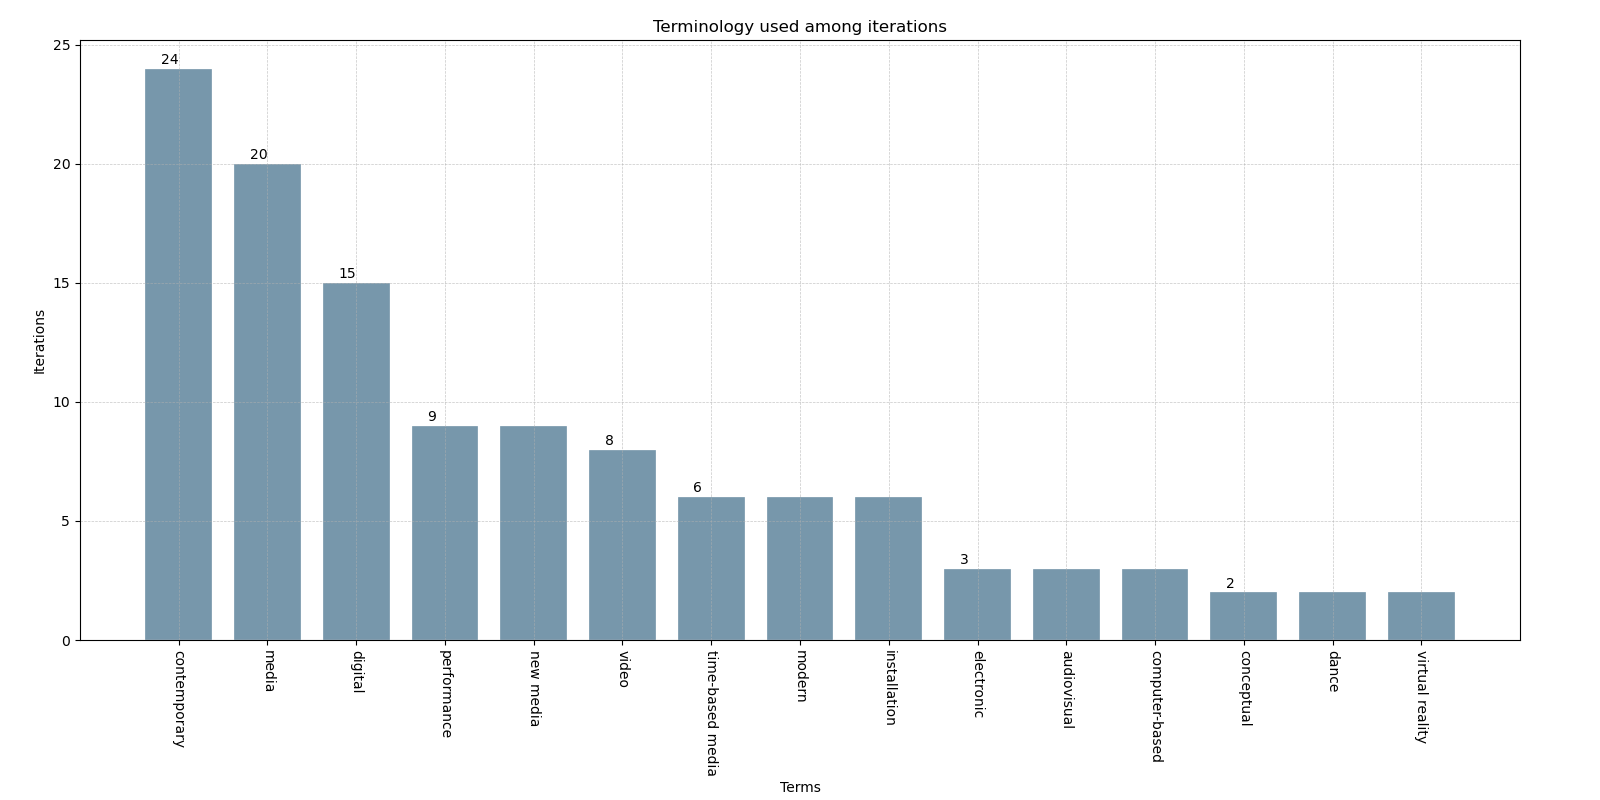
\includegraphics[width=\textwidth]{chapters/1-state_of_the_art/image/plot01-art-terms.png}
    \caption{Popularity of terms initiatives used to refer to art.}
    \label{fig:c1-terms_popularity}
\end{figure}

This data shows that many initiatives use general terms such as ``contemporary'' and ``modern'' art, which are often paired. These initiatives use these terms to embrace different genres and forms. Some examples are SMBK’s \textit{Modern Art: Who Cares?} and \textit{Interview with Artist}, the INCCA network, the web archive \textit{Basis Wien}, and many others. These initiatives include fine art, contemporary sculptures and paintings, as well as technology-based and media art.\\
The term ``media'' is the second most used. However, many initiatives have replaced this term with ``new media'' (with nine iterations) and ``time-based media'' (with six iterations), which are similar and create confusion. It is not straightforward to find a clear distinction between these terms. \textit{Monoskop} has a definition of ``media'' art \footnote{``\textit{The term media art is useful and used for artistic projects bringing up the technological, aesthetical, social, cultural, legal and political issues that come along with the emergence of new media. Since 1990s the new media have included internet, web, mobiles, wireless, GPS, and others. Media culture in this regard uses and is used by new media}” \url{https://monoskop.org/Media_art_and_culture} (last accessed 10/12/2024).}, while it only presents a few articles on ``new media'' art and ``time-based media'' art without a clear definition. Another online resource, such as the \textit{Getty Research Institute's Art \& Architecture Thesaurus}, clearly defines ``new media'' \footnote{``\textit{A genre of art-making practice involved with electronic media such as video, robotics, computer coding, and digital media in general. The term new media has been in use since the 1960s when it was applied to any non-traditional medium, initially video, which then was newly available to artists. With the rapid expansion of digital technologies, the term has come to refer to art that is by its nature electronic or digital and not merely made with with recent technological techniques}” \url{https://www.getty.edu/vow/AATFullDisplay?find=media+art&logic=AND&note=&page=1&subjectid=300435250} (last accessed 10/12/2024).} art and nothing related to ``media'' and ``time-based media'' art. A definition of ``time-based media'' art can only be found in Tate's online glossary Art Terms \footnote{``\textit{Usually time-based media are video, slide, film, audio or computer based. Part of what it means to experience the art is to watch it unfold over time according to the temporal logic of the medium as it is played back}” \url{https://www.tate.org.uk/art/art-terms/t/time-based-media} (last accessed 10/12/2024). Definition that comes from \cite{laurenson2006authenticity}.} (the context in which the term was born), which also presents a very general definition of ``new media'' art but nothing related to ``media'' art. Considering these definitions, it is possible to say that ``media'' and ``new media'' refer to the use of all media (in the Mcluhanian sense of the term) in art - emphasising novelty in the term ``new media''. ``Time-based media'' art adds temporal and processual characteristics to the former terms.\\  
Another interesting term to notice is ``electronic'', which has only three iterations related to two linked initiatives, the V2\_’s \textit{Archive and Capturing unstable Media}, and the \textit{ActiveArchive} archive. We can not find a clear definition of the term in these initiatives or the \textit{Monoskop} and Tate Terms search engines. We can see a short definition in the \textit{Getty Research Institute's Art \& Architecture Thesaurus} \footnote{``\textit{Collective term used to refer to all art works which employ electronic media or technology}” \url{https://www.getty.edu/vow/AATFullDisplay?find=electronic+art&logic=AND&note=&english=N&prev_page=1&subjectid=300387714} (last accessed 10/12/2024).}, which only specifies the electronic character of the media used. For this reason, ``electronic'' art could be juxtaposed to the three previous terms.\\
All the other collected terms refer to specific mediums and forms, such as ``digital'', ``performance'', ``video'', ``installation'', ``computer-based'', ``conceptual'', ``dance'', ``audiovisual'', and ``virtual reality''. These terms highlight the initiatives' research focus but do not elucidate the terminological confusion.

\subsubsection{Timeline}
Another critical data source is the initiation and activity periods of the initiatives, which makes it possible to represent and understand the progress of the initiatives and overall activity related to the studied subject. For this purpose, it was necessary to extract the activity period of each initiative, i.e. to obtain start and end dates. However, while almost all initiatives have a clear timeline, few do not have a clear beginning or end date, leaving much uncertainty about their timeline and progress. For this reason, these initiatives (six) were excluded from the analysis.\\
Figures~\ref{fig:c1-launched} and ~\ref{fig:c1-active} provide two different representations of the initiative's timeline, showing the number of initiatives launched (Figure~\ref{fig:c1-launched}) and the number of active initiatives (Figure~\ref{fig:c1-active}) every year. 

% \begin{figure}
%     \centering
%     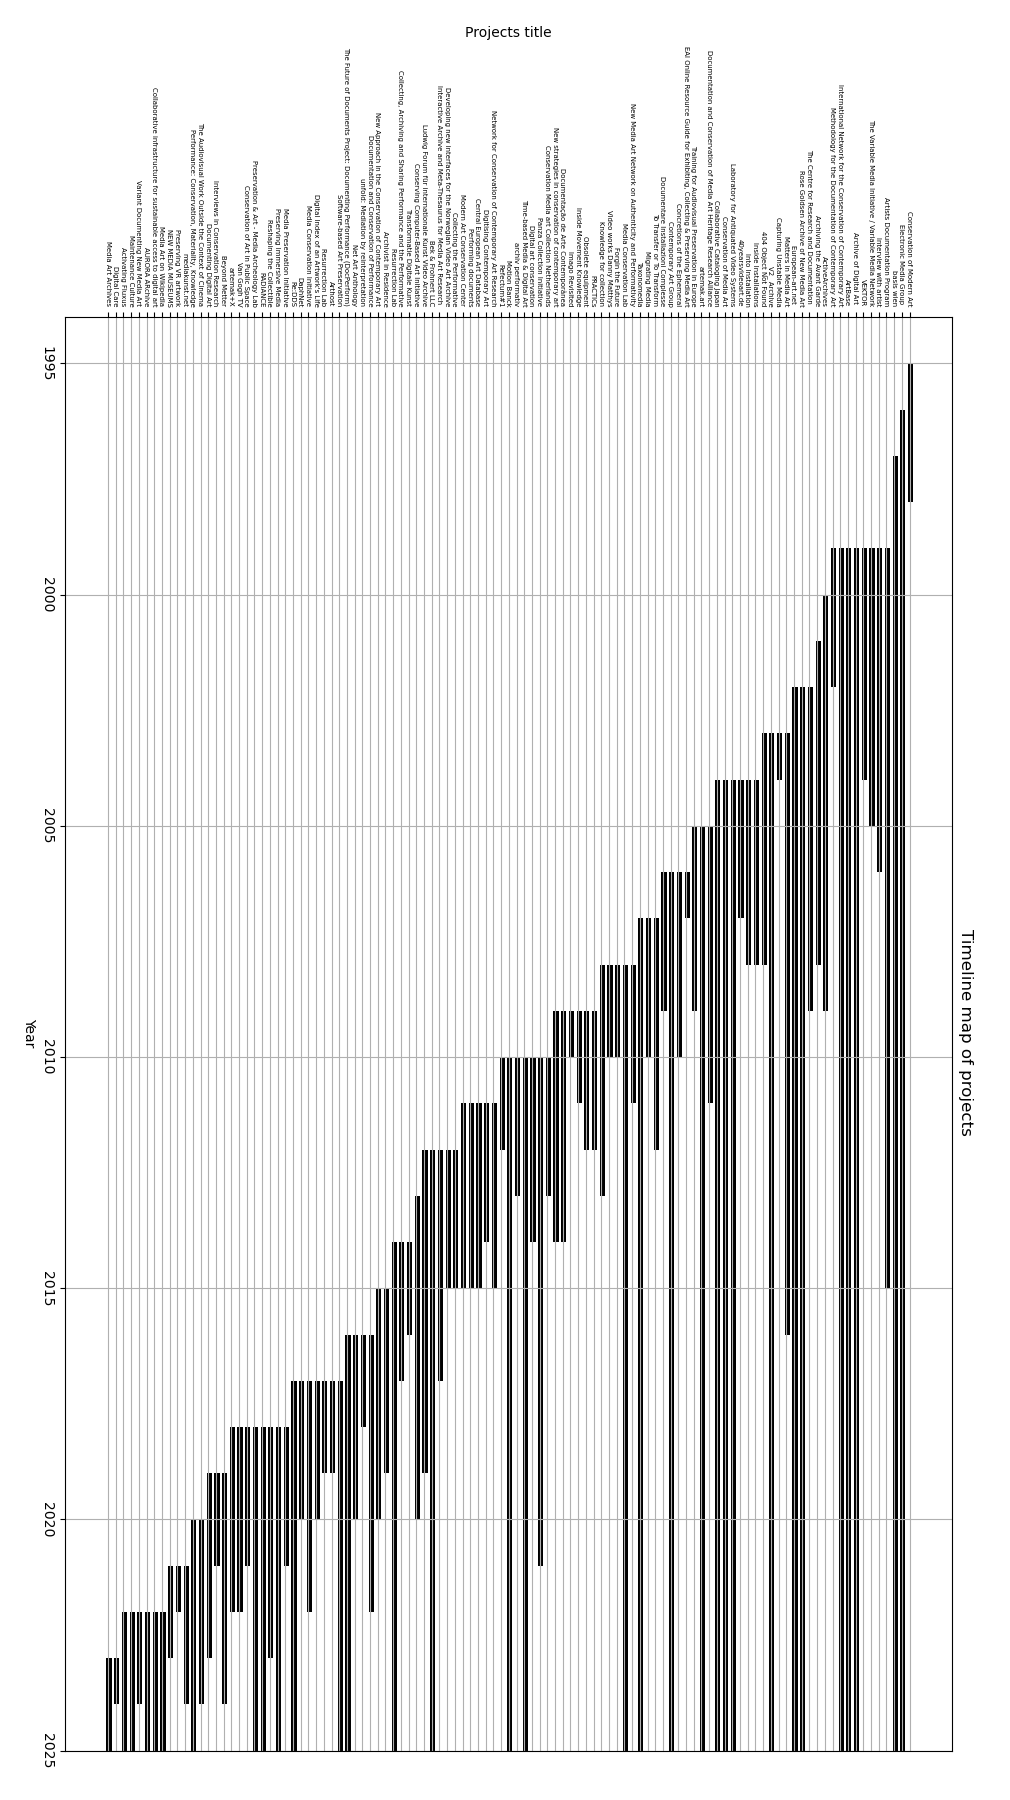
\includegraphics[width=0.9\textwidth]{chapters/1-state_of_the_art/image/plot01-timeline-vertical.png}
%     \caption{Timeline of all the initiatives, starting from 1995.}
%     \label{fig:c1-timeline}
% \end{figure}

\begin{figure}[!h]
    \centering
    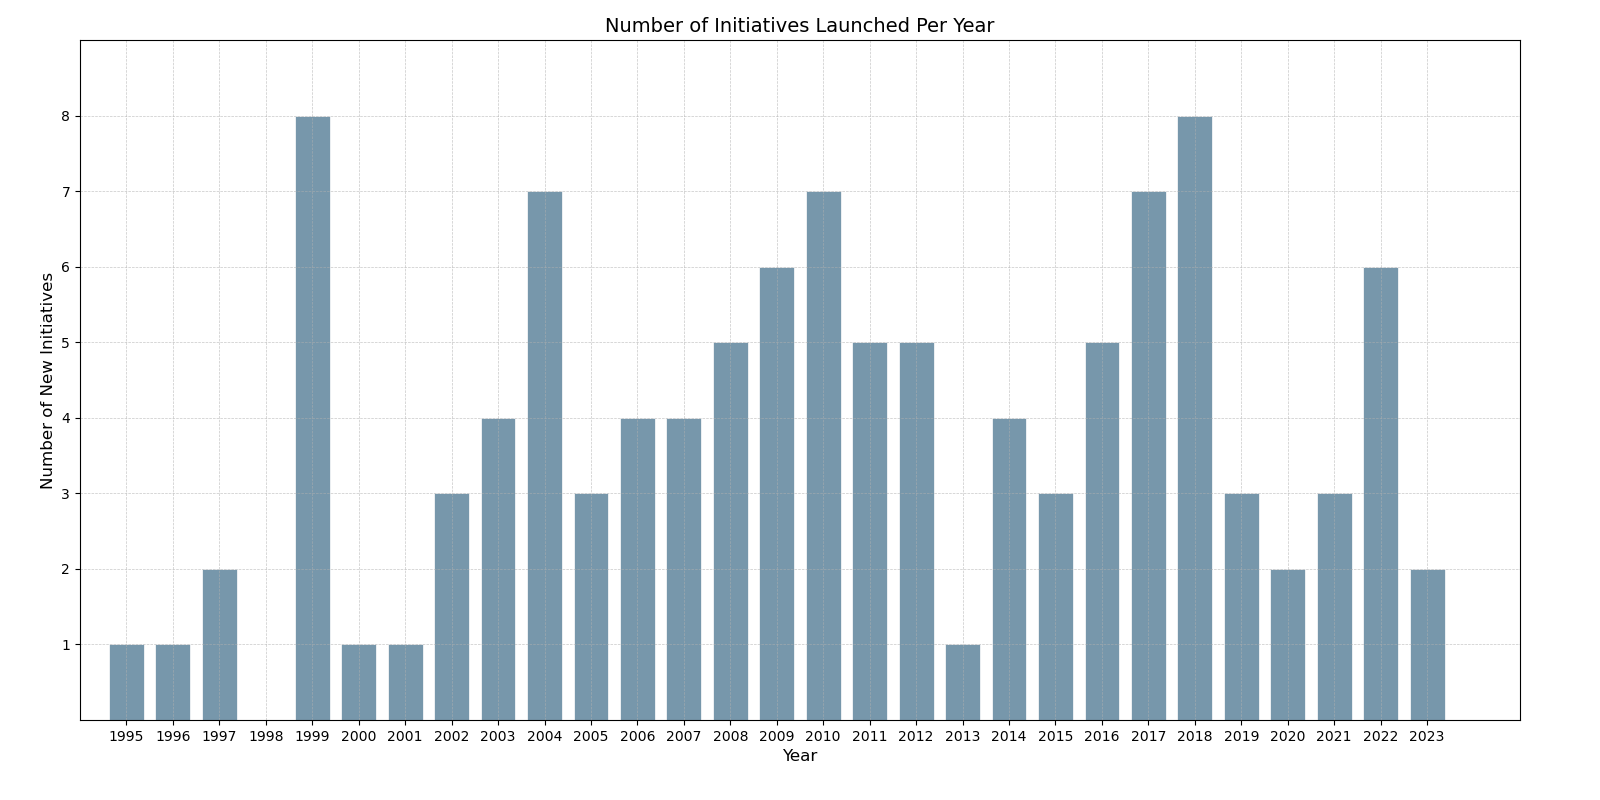
\includegraphics[width=\textwidth]{chapters/1-state_of_the_art/image/plot01-lunchedproject.png}
    \caption{Number of initiatives initiated every year since 1995.}
    \label{fig:c1-launched}
\end{figure}

\begin{figure}[!h]
    \centering
    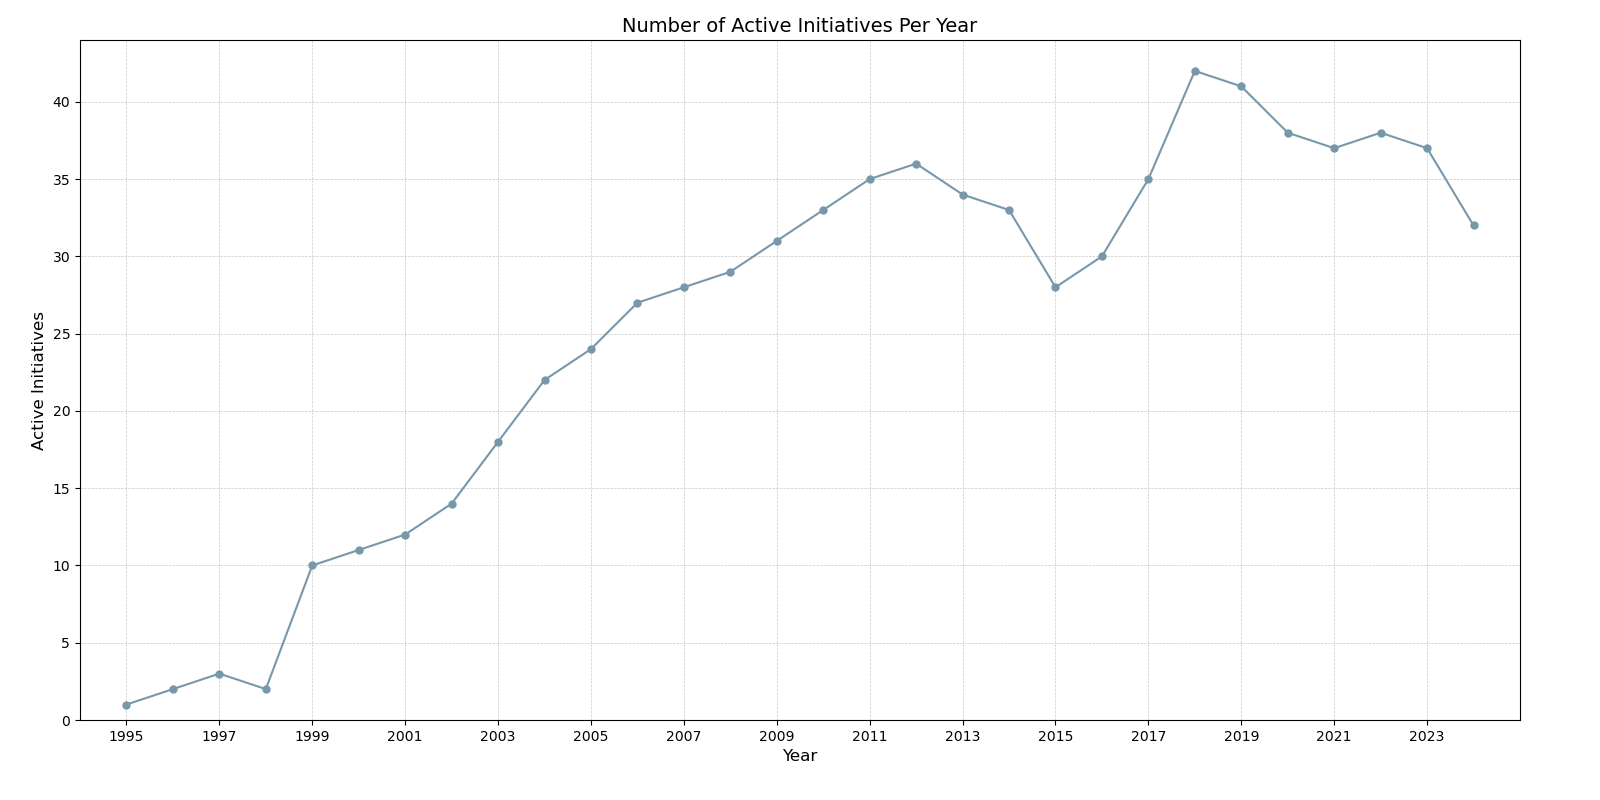
\includegraphics[width=\textwidth]{chapters/1-state_of_the_art/image/plot01-activeproject.png}
    \caption{Number of active initiatives for every year since 1995.}
    \label{fig:c1-active}
\end{figure}

Important information that we can extract from these data is the beginning of the research activity in this subject field, which started in 1995 with the well-known SBMK three-year project \textit{Conservation of Modern Art / Modern Art: Who Cares?}.\\
It is not possible to read a specific behaviour in initiative initiation (Figure~\ref{fig:c1-launched}), be it constant, increasing, or decreasing. However, we can observe some peaks in initiative initiation, especially in 1999 and 2018.\\ 
Figure~\ref{fig:c1-active} shows the overall activity in the subject field. Since its beginning in 1995, it has increased over the years and reached its maximum peak in 2018 (with 41 initiatives active in the field).\\
Another interesting data point that we can extract from the timeline representation is the average duration of the initiatives, which is 2.8 years.

\subsubsection{Geographical distribution}
Another critical piece of data collected is the geographical distribution of the initiatives. To analyse this data, we counted the countries of the organisations involved in each initiative, and the results are shown in Figure~\ref{fig:c1-geo}.\\
The first thing to notice is the dominance of projects from Western countries, mainly Europe. This data may reflect both cultural factors and potential bias in the web-based review itself. Although the INCCA network includes non-Western regional groups like INCCA Asia Pacific and INCCA Korea, these groups have fewer members and posts than the leading INCCA network. Additionally, in the \textit{Monoskop} sections ``Labs, Initiatives, Associations'' and ``Research Projects, Networks, Consortiums,'' only 4 out of 130 entities are related to non-Western projects.\\
Finally, as shown in Figure~\ref{fig_c1-geo}, the Netherlands is the most active country in this field, resulting in 88 times the total number of projects collected.

\begin{figure}[!h]
    \centering
    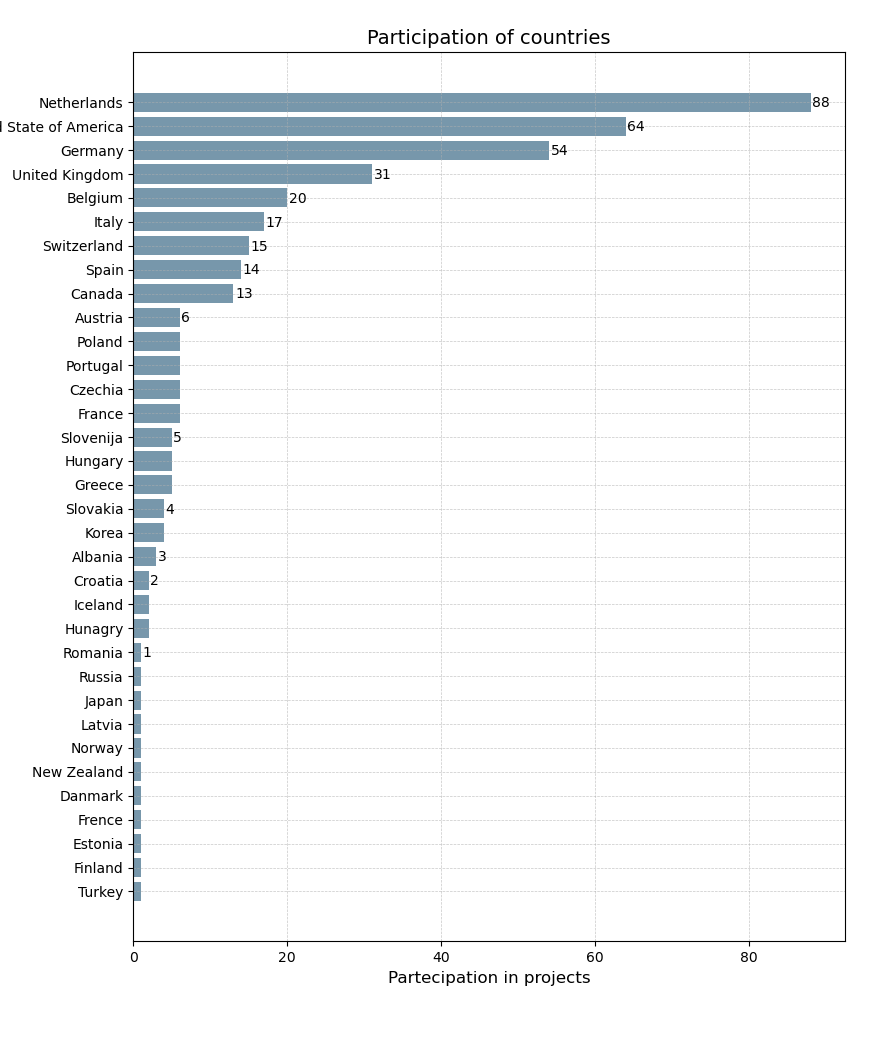
\includegraphics[width=\textwidth]{chapters/1-state_of_the_art/image/plot01-countries.png}
    \caption{Countries’ participation in conservation initiatives}
    \label{fig:c1-geo}
\end{figure}

\subsubsection{Organisations}
Related to the previous data, the leading organisations involved and their typologies are also essential pieces of data that help us understand the context in which the initiatives are developed.\\
Figure~\ref{fig:c1-org} shows the leading organisations involved, with at least five participations in different initiatives. These results perfectly reflect the previous one, with a significant prevalence of Netherlands organisations (LIMA, The Foundation for the Preservation of Modern Art, Netherland Media Art Institute, University of Amsterdam, and Cultural Heritage Agency of the Netherlands). However, Tate has the highest number of initiative participations (13).

\begin{figure}[!h]
    \centering
    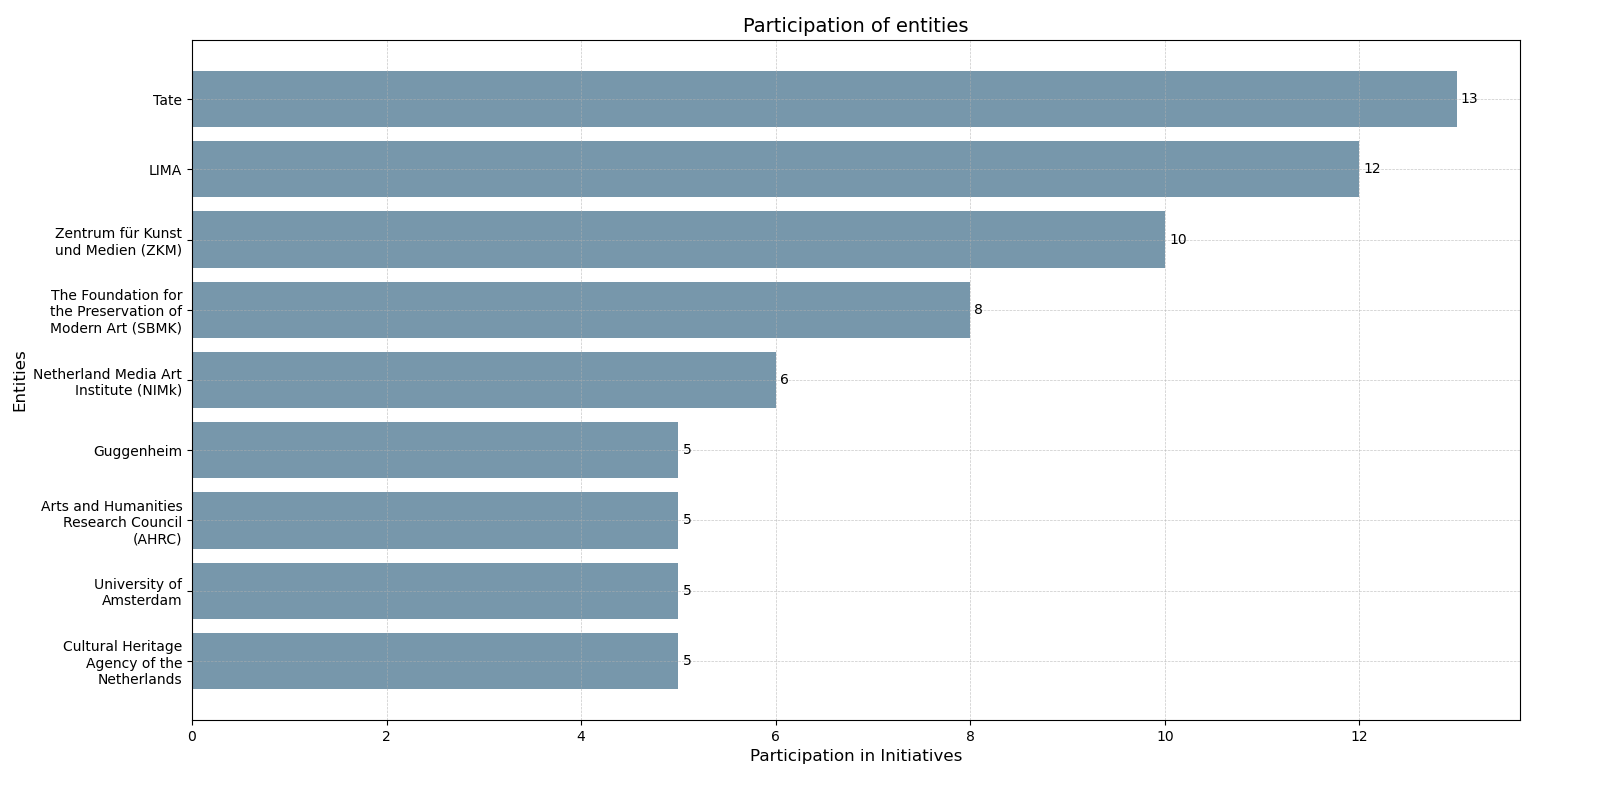
\includegraphics[width=\textwidth]{chapters/1-state_of_the_art/image/plot01-organisation.png}
    \caption{Principal organisation to participate in conservation initiatives}
    \label{fig:c1-org}
\end{figure}

Figure~\ref{fig:c1-org_type} shows the presence of different types of organisations. Although this data is particularly relevant for understanding the initiatives development context, it remains somewhat weak because of the definition of the types listed in the figure. The definition is extracted from the organisation's website on the ``home'' or ``about'' pages.\\
``Museums'' and ``universities'' (including Academies, private schools, University departments, and laboratories) remain the most fixed definitions. This data shows that universities substantially participate in these initiatives, which is interesting and important to consider. Another piece of data extracted from INCCA, although outside the scope of the analysis of initiatives, is the growth of university and academic programs specialising in conserving technology-based arts\footnote{Examples include the \textit{Still Water} program at the University of Maine in Orono, USA, founded by Joline Blais and Jon Ippolito in 2002. This program focuses on New Media art and played a key role in developing the project \textit{Forging the Future: New Tools for Variable Media Preservation}. Another example is the \textit{New Approaches in the Conservation of Contemporary Art} (NACCA) PhD program, coordinated by the Faculty of Arts and Social Sciences at Maastricht University in the Netherlands from 2015 to 2019. Additionally, the \textit{Conservation training program} at the Academy of the Arts in Bern, launched in 2021, specializes in the conservation of modern materials and media.}.\\
Other definitions, such as ``Institutes'', ``Centers'', and ``Foundations'', are more blurred. They sometimes overlap with each other and with completely different definitions, such as Museums.\\
``Institutes'' and ``centres'' are usually overlapped as definitions, so they are joined together. ``Institutes and Centers'' support and advance various aspects of art through activities like research, exhibition, conservation, education, and technology integration. These entities focus on different specialities, such as museum technology, media art, digital culture, cultural heritage, and fine art scholarship. While each institute and centre may concentrate on particular areas, they all contribute to the broader goal of promoting and conserving contemporary arts. Among the most important examples are the Zentrum für Kunst und Medien (ZKM)\footnote{The definition of ZKM given in its website: ``\textit{The ZKM | Center for Art and Media Karlsruhe is a unique cultural institution worldwide, because it is a place that expands the original tasks of the museum [...] In its work, ZKM combines research and production, exhibitions and performances, collections and archives, mediation and events. Through interdisciplinary connections of these fields of work, ZKM as an agile organization can present and produce the development of art and media of the 20th and 21st centuries}'' \url{https://zkm.de/en/about-zkm} (last accessed 10/12/2024).} and LI-MA \footnote{The definition of LI-MA given on its website: ``\textit{LI-MA plays a key role in the future-proof archiving, conservation and distribution of works from the field of media art. LI-MA is a platform for digital art and media art in Amsterdam. With years of experience in conservation and management and as a leading pioneer in the field, LI-MA plays a key role in the future-proof archiving, conservation and distribution of works from the field of media art. Specialist conservation is important to ensure that media and digital art remain accessible in the future despite rapid technological developments. As a knowledge centre, LI-MA is the link between artists, museums, cultural and scientific institutions and the public that engage with visual art and digital culture}'' \url{https://li-ma.nl/article/vision-and-mission/} (last accessed 10/12/2024).}. Sometimes, institutes and centres can own their collection and exhibition space, such as the Instituto Valenciano de Arte Moderno (IVAM) and the House of Electronic Art (HEK). The last one also defines itself as an ``interdisciplinary museum''.\\
The ``Foundation'' is another blurred and broad term. We define a ``Foundation'' as a non-profit organisation established to support charitable, educational, cultural, or other public interest activities. In the context of this specific research field, foundations usually provide grants to initiatives. Among the most important foundations are the Mellon Foundation—which founded many relevant projects such as the \textit{Artist Documentation Program} and \textit{Reshaping the Collectable}—and the Franklin Furnace Foundation—which founded projects such as \textit{The Variable Media Initiative}.\\
Another term is ``Company'', which refers to private companies focused on technologies, software, and informatic system development, such as Ubitech and FT Design Lab, and private companies specifically focused on preserving contemporary art, such as Bek \& Frohnert LLC.\\
Other voices listed in the figure are ``Government Ministries'' - support, funds, and promote initiatives-, ``Physical Archives'', ``Galleries'', ``National Institutes'' - government institutes, usually ministerial ones, specialising in cultural heritage - ``Networks'', ``Collections'', ``Miscellaneous'' - non-profit organisations not well-defined and with an extensive range of activities, such as Rhizome, Voica in Contemporary Art (VoCA), Independent Media Arts Preservation (IMAP), In Between Time (IBT) -, and ``Festival''. Other less common typologies include ``Journal'', ``Library'', ``Association'', ``Auction house'', etc. (refer to Appendix~\ref{ax:f-table_of_organisations}).

\begin{figure}[!h]
    \centering
    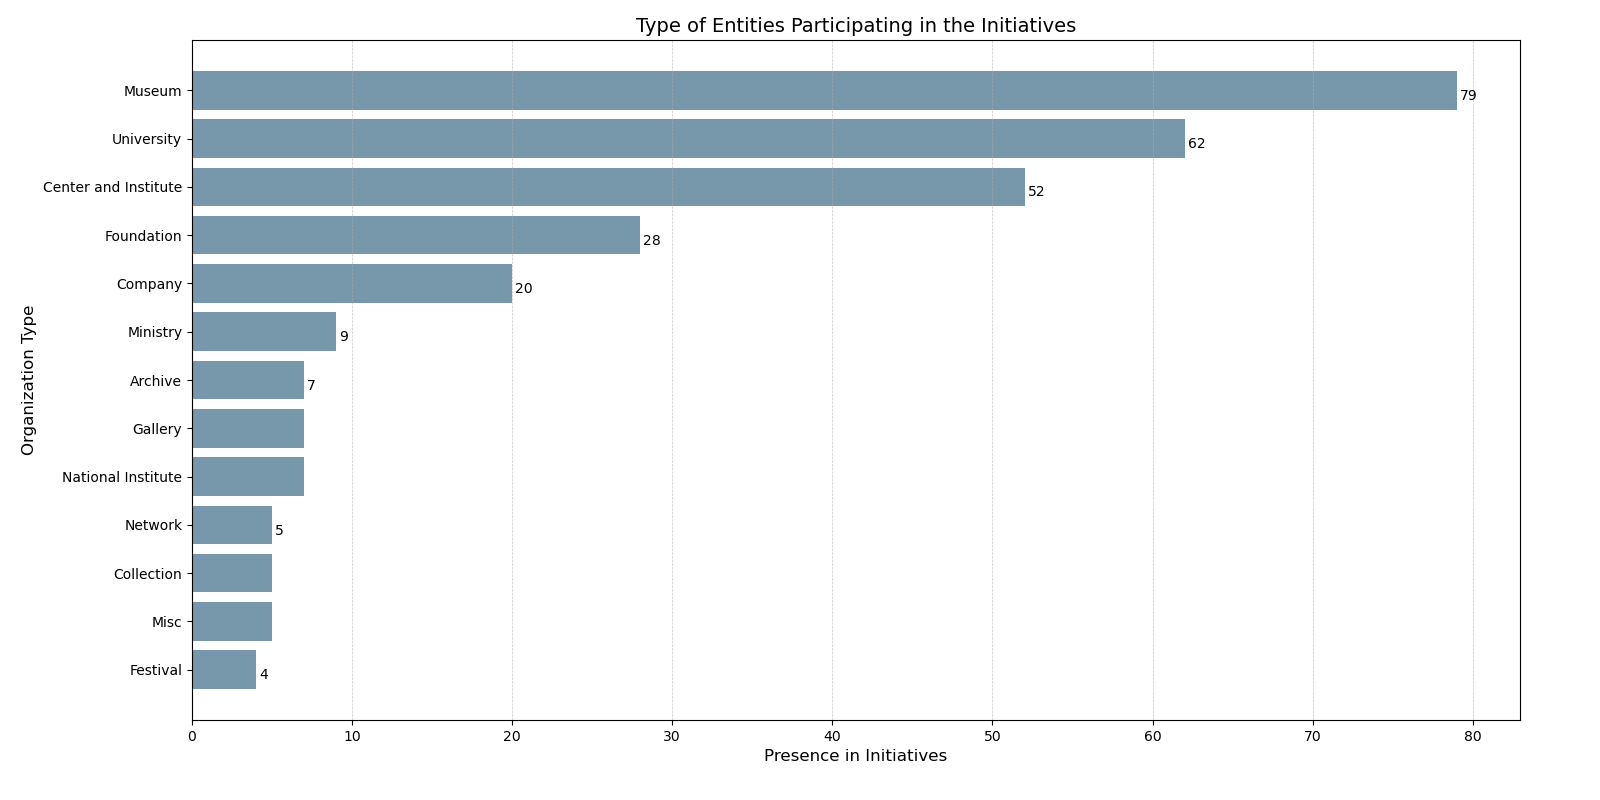
\includegraphics[width=\textwidth]{chapters/1-state_of_the_art/image/plot01-orgtypes.png}
    \caption{Participation of different types of organisation}
    \label{fig:c1-org_type}
\end{figure}

%%%%%%%%%%%%%%%%%%%%%%%% QUALITATIVE ANALYSIS

\subsection{Qualitative analysis}
Given a first quantitative overview of the initiative, a qualitative analysis involves a thematic, non-numerical, and comprehensive review of all the entries. It includes a full exploration of the website and all the resources (articles, videos, blogs, podcasts, etc.) related to each initiative.\\
As evident from the analysis below, there will be some over-mentioned initiatives. The reason is the relevant contributions and outcomes and the readily available, clear and comprehensive documentation of these initiatives. These initiatives include the \textit{Variable Media Initiative}, \textit{Matters in Media Art}, \textit{Capturing Unstable Media}, \textit{Inside Installation}, DOCAM, the \textit{EAI Online Resource Guide}, \textit{Media Conservation Lab}, \textit{Time-based Media \& Digital Art}, \textit{Media Conservation Initiative} and \textit{Media Preservation Initiative}. They present comprehensive information about the initiative and its outcomes, as well as working and intuitive websites and available external resources. Thanks to these initiatives, it was possible to define the macro thematic areas of the analysis, which were then filled in, characterised and deepened with the information collected by the other initiatives.\\
The main macro-thematic and sub-thematic areas analysed are:
\begin{itemize}
    \item Issues of preserving and documenting time-based media art
    \item Limitations of traditional preservation strategies
    \item New preservation strategies
    \item Documentation
    \begin{itemize}
        \item Documentation process
        \item Identity report
        \item Iteration report
        \item Condition report
        \item Documentation models
        \item Thesaurus and Glossary
        \item Interview
    \end{itemize}
\end{itemize}
\subsubsection{Issues of preserving and documenting time-based media art}
The first analysed macro-thematic area has been the incipit of all these initiatives, namely the challenges of conserving and documenting live media art. All the initiatives are born to find practical or theoretical solutions to specific problems.\\ 
Challenges concerning the preservation of live media art can be divided into distinct and hierarchical classes. These challenges encompass the \textit{creative process}, the \textit{intrinsic} and \textit{extrinsic} features of artworks, and the \textit{derivative issues} of conservation. This subdivision allows us to better describe the problems of conserving and documenting live media art in an organised way.\\
Figure~\ref{fig:c1-issues} provides an overview of the hierarchical structure of these features and issues. \textit{Intrinsic} refers to factors inherent to artworks themselves (physical and contextual) and the experience they produce. \textit{Extrinsic} refers to subsequent consequences, extending beyond the immediate realm of the artwork and its experiential dimensions. The \textit{creative process} refers to the development and production phase of the artwork. Finally, the \textit{derivative issues}—derived from the artwork features–summarise all the problems challenging the preservation of live media art. 

\begin{figure}[!h]
    \centering
    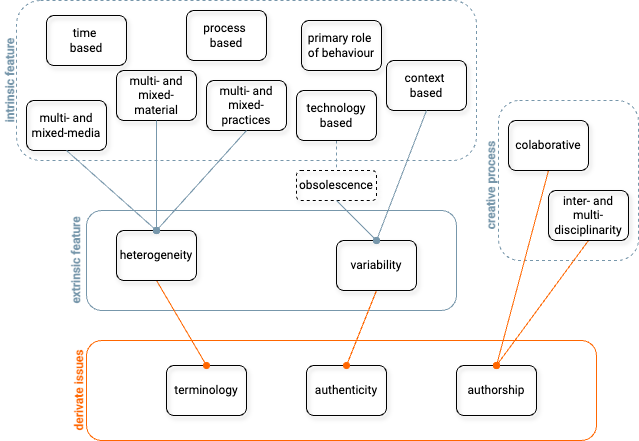
\includegraphics[width=\textwidth]{chapters/1-state_of_the_art/image/graph-issues.png}
    \caption{The diagram represents the \textit{intrinsic}, \textit{extrinsic}, and the \textit{creative process} features of live media artworks and the \textit{derivative issues} related to their preservation.}
    \label{fig:c1-issues}
\end{figure}

\paragraph*{Intrinsic}
The main \textit{intrinsic} features of the artworks considered by the initiative studied are their time and process nature, which classifies them as ephemeral [\textbf{CIAO}, \textbf{Performance conservation}, \textbf{Capturing Unstable Media}]. Both performance and installation exist only when performed or installed, and during their existence time frame, they produce an experience that unfolds over time. For this reason, most initiatives consider live media artworks as \textit{allographic} [\textbf{Guggenheim}], like other art forms such as music, dance and theatre.\\
Live media artworks use a wide variety of materials, tools, methods, and practices often linked and mixed between them and whose significance is unique and inscribed in the individual work [\textbf{Conservation of Modern Art}, \textbf{Capturing Unstable Media}, \textbf{Preserving Immersive Media}, \textbf{CIAO}]. Artworks may be analogue or digital, are often multimedia-based, and contain images and sound that may also be analogue or digital, fixed or moving, pre-existing or directly generated, and so on [\textbf{DOCAM}].\\
They are based on technology and use various devices, usually adapted or created by artists and collaborators. Technologies range from more to less conventional and sometimes cutting-edge ones, and they can include film, video, computers, electromechanics, robotics, web, networking, and so on [\textbf{Inside Installations}, \textbf{DOCAM}, \textbf{EAI}, \textbf{Documentação de Arte Contemporânea}]. The use of technology in artworks is often unconventional, exploring new possibilities, bugs and anomalies [\textbf{EAI}].\\
Another important inherent factor is that live media artworks are often based on the context of the original manifestation. They are usually developed with a specific and strict relationship with the space they occupy and the time of their production. Moving artworks to another context, location, and time can profoundly alter their meaning [\textbf{Capturing Unstable Media}, \textbf{Inside Installation}, \textbf{Documentação de Arte Contemporânea}, \textbf{NeCCAR}]. Especially for performance-based artwork, there is also a strong relation with the original performer(s) (very usually the author) [\textbf{NeCCAR}, \textbf{Collecting the performative}, \textbf{Collecting the performative}].\\
Most importantly, all these artworks show a relevant shift in the creation process, from the object and its physical materiality to the emphasis on the concept [\textbf{Documentação de Arte Contemporânea}] and the primary role of behaviour.\\
The primary role of the artwork’s behaviour, which is the live experience activated by the relationship of the artwork’s presence and the context (including the surrounding space, the moment, and the performers and audiences), seems to be accepted by most initiatives. As one of the first and groundbreaking initiatives in the field, the \textit{Variable Media Initiative} highlights the importance of behaviour, classifying its different forms in art as contained, installed, performed, interactive, reproduced, interchangeable, encoded, and networked [\textbf{Variable Media Initiative}]. The DOCAM research alliance defines behaviours as interactive, processual, procedural, programmatic, distributed, hybrid, migrant, ethereal, collaborative, or a mix [\textbf{DOCAM}].\\
Among these behaviours, which often overlap and whose definitions are usually blurred, the interactivity is mainly highlighted by the initiatives. The ``acclaimed'' interactivity (as defined in the \textit{Capturing Unstable Media}) allows the user to interact with the artwork, manipulate or take home components of a physical work [\textbf{Variable Media Initiative}], and in general and most importantly, allow people to influence input and output and become active participants rather than spectators [\textbf{Capturing Unstable Media}].

\paragraph*{Extrinsic}
All these \textit{intrinsic} characteristics generate \textit{extrinsic} features, which determine the main issues in preserving live media art. We can distinguish two macro-factors: heterogeneity and variability.\\
Contexts, technologies and mixes of material, practices and media are combined in an individual and original way for each artwork. That means every artwork is a world of its own, with its components, appearance and experience. In other words, artworks are heterogeneous, making it difficult to find standard practices and terminologies to describe them. 
On the other hand, variability is a more complex feature that makes the artwork unstable and in a constant transformation process: a transient process rather than a fixed object [\textbf{Methodology for the Documentation of Contemporary Art}, \textbf{DOCAM}]. This variability is primarily the result of context- and technological-based features of artworks.\\
Since each artwork has a relationship with the context (e.g., the surrounding space of a specific location), when it is ``re-presented'' or ``re-interpreted,'' it should be adapted to the circumstances of the new context, appearing differently each time [\textbf{Concretions of the Ephemeral}]. Therefore, each manifestation may be considered a different representation of the artwork [\textbf{CCBA}] or, from another perspective, based on a mutable context [\textbf{EAI}].\\
However, the technological feature of live media art determines the central problematic aspect of variability, which is also the main challenge of most initiatives. Live media artworks suffer from the fragility and ageing of the technologies involved, which are difficult to repair or replace because of the rapidly evolving technological landscape [\textbf{Variable Media Initiative},\textbf{ Capturing Unstable Media}, \textbf{DOCAM}, \textbf{Inside Installations}, \textbf{Obsolete Equipment}, \textbf{ActiveArchives}, \textbf{Concretions of the Ephemeral}, \textbf{Archivist in residence}, \textbf{Software-based art preservation}, \textbf{CCBA}, \textbf{UNFOLD}]. Therefore, like everyday technology such as display equipment, smartphones, computers, and home appliances, even artworks quickly become obsolete. So, to present the artwork again, some components have to be repaired but usually have to be replaced with new technologies that can reproduce the behaviour of the old ones. Although this operation is not always possible, mainly when the meaning and goal of the works lie in their material components [\textbf{DOCAM}], it is still controversial from the perspective of the ethics of traditional restoration [Concretions of the Ephemeral].\\
Finally, the variability of the artworks should also consider perishable [\textbf{Documentação de Arte Contemporânea}], degradable [\textbf{NeCCAR}], and consumable materials.

\paragraph*{Creative process}
Another issue involves the \textit{creative process}. The V2\_’s \textit{Capturing Unstable Media} initiative focuses on this. Instead of viewing artworks as final ``precious originals'' created by a single ``artist's genius,'' we need to consider their ongoing process and ``distributed authorship.'' The \textit{Capturing Unstable Media} initiative suggests calling electronic artworks ``projects'' to reflect this shift. These projects are part of a larger entity or process, including research, development, festivals, and exhibitions. They use various materials and methods and involve interdisciplinary or multidisciplinary collaborations. Projects often do not end after their first showing; they have multiple stages with different people contributing. The results come from a team effort between artists, scientists, engineers, and designers. Together, these teams create artistic and cultural expressions within broader contexts like research themes, performances, and festivals, known as \textit{aR\&D} (artistic Research and Development) [\textbf{Capturing Unstable Media}].

\paragraph*{Derived}
So, considering these \textit{intrinsic} and \textit{extrinsic} features as well as the issues related to the \textit{creative process}, the primary layer of live media art preservation issues arises, which includes the authenticity and the authorship of the artworks.
One of the most theoretical and practical challenges of live media art conservation is the notion of the ``original'' [\textbf{inside installations}] and, therefore, determining the authenticity. The behaviour-based character, the ephemeral nature, and the variability of the art are thrown into crisis by this fundamental notion of ``originality'' that is the basement for conservators, museums, and collectors. What is essential to determine the origins and authenticity of the work? What parts of it should be preserved, transformed or re-created? [\textbf{Inside installation}]\\ 
Another issue concerns the authorship and the artwork's intellectual properties (copyrights). Artworks are usually born from multi- and inter-disciplinary collaborations; pieces of software and hardware are reused among different artworks; especially networking and participative artwork arise from the active collaboration with the audience. Intellectual property is no longer a located quality (for one or a small group of individuals) but rather a spread factor, usually involving people unknown to each other. As mentioned, the Capturing Unstable Media initiative called this property ``distributed authorship'' [\textbf{Capturing Unstable Media}].\\
A last problem that arises from the heterogeneity factor is terminology, which refers to more than just the perspective analysed above—according to the definition of this art—but also the description of such art. Proper description and definition are required for many different elements, including the heterogeneity of behaviours, components, media, materials, etc. 

\subsubsection{Comparison with traditional preservation strategies}
Given these features and issues, it is evident that traditional preservation strategies are no longer suitable for live media art. Traditionally, conservation conceives of artworks and their documentation as a function of their material presence, which must remain stable and fixed [\textbf{Capturing Unstable Media},\textbf{ Inside Installation}, \textbf{Performance conservation}]. Through this perspective, originality, authenticity, and authorship are easily inscribed in the materiality of artworks since the object of preservation is \textit{autographic} [\textbf{Guggenheim}].\\
Almost all the initiatives dealing with these issues propose a shift in the preservation paradigm, replacing the primary role of materiality with behaviour [\textbf{Variable Media initiative}, \textbf{Inside Installation}, \textbf{DOCAM}, \textbf{Archiv performativ}]. However, this shift generates a complex discussion around one of the main derived issues: authenticity. This concept should be revised or abandoned. For many initiatives, the idea of authenticity should not be ``sacrificed'' to the variability of the artwork but rather reformulated. Live media artworks’ authenticity should be understood as a process rather than a single and fixed quality [\textbf{Capture Unstable Media}, \textbf{Variable Media Initiative}, \textbf{ZKM}] or conceived as mutable and multiple \cite{castriota2018centres}[\textbf{NACCA}]. In other cases, new preservation strategies should replace the notion of ``originality'' and then authenticity with the ``identity of the artwork'' [\textbf{Guggenheim}]. Only this quality of the artwork should be preserved intact. 

\begin{quote}
The identity of a media artwork, however, is not necessarily compromised by the damage and replacement of its physical equipment. In fact, its integrity might be more endangered by representing the work poorly—e.g., by choosing suboptimal video compression, by accepting compromising light and sound conditions, or by migrating the piece to a technology that does not provide the artist-intended and work-defining properties. 
[\textbf{Guggenheim}]
\end{quote}

Beyond these views on authenticity, almost all initiatives focus on developing two main aspects: restoration and documentation.\\
Most of the proposed conservation strategies move toward ``medium-independent'' approaches [\textbf{Variable Media Initiative}]. That does not mean abandoning the physical properties of the artworks altogether, but firstly consider the ``behaviour'' and look at this property in relation to the component and their functions [\textbf{Variable Media Initiative}] by defining the acceptable degree of changes that an artwork may undergo in response to different display environments, technological developments, curatorial and exhibition-design concepts, or technicians’ preferences [\textbf{Guggenheim}]. It is, therefore, vital to determine what constitutes the work, especially the relationship between the behaviour and the materiality, and under what circumstances it can continue to be considered the same work [\textbf{DOCAM}]. 

\begin{quote}
To make an informed assessment, the conservator must fully understand the function and characteristics of involved technologies and identify their specific impact on the artwork’s aesthetic, conceptual, and historical identity. 
[\textbf{Guggenheim}]    
\end{quote}

In order to get a clear understanding of the artwork, we need a set of specific information and a well-structured documentation model with which to collect all the data. Since the aim is the ``behaviour'', information about components is not enough, ``we need artists'' [\textbf{Variable Media Initiative}]. Collaboration with the artist is one of the first (if not the primary) fundamental elements of the new conservation strategies [\textbf{ADP}, \textbf{Interview with Artist}, \textbf{Variable Media Initiative}, \textbf{Inside Installation}, \textbf{EAI}, \textbf{Archiv Performativ}, \textbf{Media Preservation Initiative}]. Questionnaires and interviews are fundamental to getting the intent or a statement regarding the artwork, understanding the relationship between ``behaviour'' and components, and determining how their creation should evolve. For many initiatives, artists are not enough: if we consider the ``distributed authorship'', all the production and development environment should be involved [\textbf{Capturing Unstable Media}]; if we consider the interactivity and participatory aspect of many artworks, even audiences should be taken into account \cite{muller2008experience}[\textbf{The Centre for Research and Documentation }].\\ 
Other types of information are related to practical ones, such as instructions and scores (to make an analogy with music). How do the components work, how are they related to each other, and how are they activated during the performance or installation?\\
All this collected information should be organised in a dedicated administrative documentation model. The documentation and how it is organised are essential for preserving live media artworks [\textbf{Guggenheim}]. With a clear and compelling documentation model, it is possible to describe artworks from many perspectives, from their identity, authorship, inner or outer relations, vulnerabilities, conditions, damage, and conservation treatments. A typical document of many new documentation models is the ``iteration record,'' which allows them to record the variability of artworks over their manifestations.

\subsubsection{Preservation Strategies}
One of the first results shared by many initiatives is the new restoration and preservation concepts. However, before the analysed initiatives, it is important to mention Bill Viola, one of the first to give a clear perspective on conserving live media art. In its 1999 over mentioned article, \textit{Permanent Impermanence} \cite{viola1999permanent} -which includes the famous analogy between contemporary art and music, introducing the concept of ``score'' inside visual art production- the artist considers the obsolescence of media and names two fundamental macro-categories of preservation approach, the \textit{purist, original-technology-at- all-costs approach} and the \textit{adapted/updated technology approach}.\\
Starting from these categories, The Variable Media Initiative was one of the first initiatives to give a clear distinction between preservation strategies and classified them as:
\begin{itemize}
    \item \textit{Storage}: the most conservative collecting strategy, which means physically storing a work.
    \item \textit{Emulation}: imitating the original look of the piece by entirely different means.
    \item \textit{Migration}: upgrading artworks’ equipment and source material. 
    \item \textit{Reinterpretation}: the most radical preservation strategy is to reinterpret the work each time it is re-created.
\end{itemize}
These remain the main distinctions of live media art preservation strategies adopted by most initiatives. It is possible to find new terms, such as \textit{reconstruction} in the DOCAM research alliance, \textit{encapsulation} in the \textit{Online Resource Guide for Exhibition}, \textit{physical repair} in the Guggenheim \textit{Media Conservation Lab}, and others that can always be grouped as sub-categories inside one of the four main categories. It is also possible to find new categories, such as \textit{virtualisation} (at the base of the \textit{Beyond Matter} project or \textit{To Transfer or To Transform}), which propose a new way of restoration through virtual and augmented reality systems.\\
However, some initiatives propose other perspectives on live media art preservation. The project \textit{Archiv Performativ} (2010-2012) - based on performance art - proposes the term \textit{transcription}, which includes any level of artwork transmission, from historical faithfulness to interpretative translation. They even introduce the term \textit{reinscribing}, which stays for ``\textit{a clear eclipsing of an intentional or specific aspect of a work}''. We reinscribe one or more elements of artwork when they are closely bonded to a specific context (e.g. historical context) and no longer intact in an artefact or transcription but evoke a completely different experience.\\
LI-MA’s \textit{UNFOLD} project emphasises the importance of \textit{reinterpretation}. Taking up the analogy with ephemeral arts, it defines re-interpretation as a process in which the work is translated into a new context through only documentation, scripts, memories, or scores.  In these arts, \textit{reinterpretation} becomes an integral part of artistic practice, as should also be the case with media art. Indeed, the ``\textit{reinterpretation of media art can contribute to the preservation and better understanding of the work}'' [\textbf{UNFOLD}].\\
Many initiatives emphasise the importance of making the right decisions to preserve the artwork [\textbf{Guggenheim}, \textbf{DOCAM}]. The strategy used, whether it is storage with physical repair, migration, emulation, or reinterpretation, should be selected and applied after a comprehensive assessment of the artwork. For this purpose, the DOCAM project proposes the \textit{Decision Tree}, a restoration tool that identifies problems and potential solutions associated with preserving works with technological components.\\
\begin{quote}
    The tool facilitates decision making by helping users focus on the aspects of a work that relate to its integrity and authenticity while reflecting on how these aspects are impacted by the work’s technological components. 
    [\textbf{DOCAM}]
\end{quote}

This tool is based on a series of questions (e.g. ``\textit{Is the equipment visible?}'',  ``\textit{Does it have a particular significance?}'', ``\textit{What is the artist’s point of view?}'') whose answers lead to identifying the best restoration option to apply to a specific artwork.

\subsubsection{Documentation}
In general, we can observe that documentation often plays a central and primary role in the initiatives analysed.  Documentation is essential for the preservation [\textbf{Guggenheim}]. As better suggested by the DOCAM research alliance, documentation is a source of information that has many roles depending on its use and timing [\textbf{DOCAM}]:

\begin{itemize}
    \item Documentation servers the artists and collaborators in the production phase;
    \item As its development progresses, the documentation plays an essential role in the mediation, dissemination and history of the art;
    \item Next, the documentation allows a variety of actions and activities, such as the artwork installation, preservation and restoration;
    \item Over time, thanks to the documentation, the re-installation and re-contextualization may be carried out;
    \item Later still, documentation may serve to compensate for various “losses” or deteriorations suffered by the work;
    \item Ultimately, the documentation will survive the work, becoming its historical witness and sometimes supplementing any remaining fragments or relics.
\end{itemize}

Initiatives’ efforts have been oriented toward the development and standardisation of:

\begin{itemize}
    \item \textit{Processes of documentation}, from acquiring, cataloguing, and archiving to restoring, preserving, and loaning the artworks; 
    \item \textit{Documentation templates} to document the acquisition condition, the possible damages, the copyrights, the identity and the iterations of artworks;
    \item \textit{Glossaries and thesaurus} with which to describe artworks and their components;
    \item \textit{Documentation model} with which to organise and archive data about the artworks;
    \item \textit{Interview} for artists, collaborators, and audiences.
\end{itemize}

\paragraph*{Documentation process}\\
The documentation processes are thought to be used by museums and collectors. Summarising all the outcomes of the initiatives, it is possible to divide this process into five main steps:

\begin{enumerate}
    \item The \textit{Pre-Acquisition} is described as the first and one of the most important steps in the documentation process [\textbf{DOCAM}, \textbf{Matters in Media Art}, \textbf{MoMa}] since it is thought to gather as much information as possible before deciding whether or not to acquire the artwork. During this step, collectors and conservators must collect information about the artwork and its maintenance. Significant aspects to define during this step are the financial aspect (from the loan fees to the cost of the presentation and preservation), the copyright, risks for the conservation, and the artist collaboration [\textbf{DOCAM}].\\
    The Matters In Media Art project defined three steps curators and collectors should follow to accomplish the pre-acquisition process: a) \textit{What is it?} b) \textit{Explore Deeper}, and c) \textit{Assemble Expertise} [\textbf{Matters in Media Art}]. The Media Conservation Lab at MoMa published a questionnaire that should guide the pre-acquisition process [\textbf{MoMa}]. 
    \item The \textit{Acquisition} step is the most important and delicate step regarding documentation [\textbf{Matters in Media Art}, \textbf{DOCAM}, \textbf{MoMa}, \textbf{TBMA}, \textbf{MPI}, \textbf{Guggenheim}, \textbf{EAI}]. The acquisition involves contractual documents (purchase agreement, or a deed of gift, a copyright licence, and acquisition’s terms and conditions) [\textbf{Matters in Media Art}] and the fulfilment of important pieces of information, such as the identity report, the condition report, the definition of the parameters and so on. Interviews with artists can be conducted during this step. Some initiatives have designed a questionnaire to be fulfilled in this step [\textbf{DOCAM}].
    \item \textit{Cataloguing} is the step in which all the information and documentation gathered during the acquisition process must be archived into a collection management system [\textbf{Matters in Media Art}, \textbf{DOCAM}]. This is where templates, metadata structures and ontologies, and new vocabulary systems define original documentation models designed to maintain knowledge of the artwork and aid its preservation.\\
    \item The \textit{Preservation} step is related to the constant care inside the collection or museum and the new exhibition of artworks. This step involves the decision-making models [\textbf{Conservation of Modern Art}, \textbf{DOCAM}] and the abovementioned preservation strategies.\\
    Every action taken to preserve the artwork must be documented. For this purpose, many initiatives have developed an iteration report [\textbf{DOCAM}, \textbf{MoMa}, \textbf{TBMA}, \textbf{MPI}, \textbf{Guggenheim}] to gather as much information as possible about applied preservation strategies. Consequently, many original collection management systems for live media art are structured to include the iterations’ history of artworks [\textbf{DOCAM}, \textbf{MoMa}, \textbf{Capturing Unstable Media}, \textbf{Guggenheim}, \textbf{TBMA}, \textbf{MPI}].\\
    \item Finally, the \textit{Loan} is another important part of the collected artwork, involving a series of templates and contractual documents that must be completed by both parties, the owner and the borrower [\textbf{Matters in Media Art}, \textbf{MoMa}, \textbf{TBMA}, \textbf{MPI}]. The owner should also verify that the planned exhibition can fulfil the artwork requirements for both the maintenance (avoiding situations that can raise risks) and the installation (e.g. verifying that the space is appropriate for the installation). Furthermore, each exhibition is a new iteration; therefore, the iteration report should be completed even now.
\end{enumerate}

\paragraph*{Documentation template and reports}\\

Collecting and maintaining live media artwork involves filling out many documents with defined purposes. Some documentation templates, developed according to individual collection management systems, are shared among the initiatives. These are the \textit{identity report}, the \textit{iteration report}, and the condition report.\\
\newline
The \textit{identity report} captures the essence of the artwork by detailing its original components and addressing the intrinsic variability of live media art. It is designed to collect comprehensive information about the artwork and its history, from the creative process to its most recent iteration.\\
The \textit{identity report} links back to the discussion about the authenticity of live media artworks. The main conceptual background of this report is the replacement of the ``original'' -and so authenticity- with the ``identity of the artwork'', the principal aspect that has to be conserved. Indeed, the identity is not necessarily compromised by damaging and replacing its physical equipment [\textbf{Guggenheim}]. As mentioned, this is a shared solution among many initiatives for facing live media art variability.\\
An example of an \textit{identity report} is that used at the MoMa’s \textit{Media Conservation Laboratory}. This report template is divided into seven information sections:

\begin{itemize}
    \item The \textit{Artwork identification} comprehends the main information about the artwork, such as the title, the artist's name, the year of production, the medium line, the edition, and a representative picture of the artwork.
    \item The \textit{Identify the Artwork} section focuses on an in-depth artwork description from a curatorial and artistic perspective. In addition to a general description, this section includes a definition of the essential qualities and intended experiences of the work, as well as its technical and exhibition aspects regarding the technologies and media involved. Furthermore, this section comprises information about variability and which components and parameters can or can not change.
    \item The \textit{History of Exhibitions and Iterations} section lists all the iterations of the artworks with related information such as date, title, venue, pictures, and whether they were successful from the artist’s perspective.
    \item The \textit{Anatomy of the Artwork} section includes a list of playback and display equipment and installation components with a series of defined and necessary information (significant properties; categorisation of equipment as dedicated, non-dedicated, shared, and obsolete; example makes and models preferred; and work-defining	properties).
    \item The \textit{Risks and Resources} section classifies risks based on the meaning and significance of each component and defines the preferred conservation strategies, including the artist’s statement. Furthermore, it lists the necessary resources for conservation, such as suppliers of dependent equipment and components, as well as resources of required know-how and services.
    \item The \textit{Installation Parameters} section covers another important aspect of the artwork, which regards the necessary information for installing it, such as the required space, the layout of the equipment and components between them and within the space, and the required expertise for setting up the work.
    \item The \textit{Technical Requirements and Parameters} section expands on information about the installation and focuses on technical aspects that are less related to the work itself but more to its operation. The section includes information about the wires, the power, the details about the syncs and so on.
\end{itemize}

Other \textit{identity report} templates explicitly include specific fields such as the \textit{statement of significance}, which defines what is essential about the work and aims to guide future decisions about the ongoing care and display of the work [\textbf{TBMA}, \textbf{Matters in Media Art}], and the \textit{conservation plan}, which responds to risks with practical information about preservation strategies. \\
\newline
The \textit{iteration report} is a fundamental documentation template, unique in preservation practice in general and created exclusively for live media art. The report monitors and manages the periodic change of live media artworks. The variability of the artwork, which materialises periodically every time the work is presented or changed in function of its conservation, must be documented. This documentation should be done for each iteration separately \cite{phillips2015reporting} in order to identify each intervention and define the dynamic life cycle of the artwork. The iteration report is critical for tracking the variability of the artwork since its first presentation without losing its original form (even if only in a documentation form).\\
The \textit{iteration report} should be compiled every time the artwork is presented, and the information required–as shared among many initiatives’ templates–regarding the event, the exhibition and the practical installation details. An example is the template used by the Guggenheim’s \textit{Media Conservation Laboratory}, which is defined by 12 detailed fields:

\begin{itemize}
    \item \textit{Artwork information} (title, artist, year, etc.);
    \item \textit{Exhibition information} (title, date, and venue);
    \item \textit{Iteration information} which includes much information regarding who installed, supervised and curated the installation of the artwork, whether the artist was present, different evaluations of the installations, photos of the installed work and the produced documentation; 
    \item \textit{Space information }concerns the description of the space where the work was installed. In addition to a simple description, the field requires pictures and names of people who gave and approved a particular installation choice. 
    \item \textit{Exhibition copies};
    \item Description of the \textit{equipment} used in the installation with the motivations (decision-making) and names of people who chose to use a specific equipment; 
    \item Description of \textit{other installation components} used for installing the work with the motivations (decision-making) and names of people who chose to use a specific component;
    \item Information about the \textit{technical setup}, such as cabling, setting, synching, powering, etc, with the motivations (decision-making) and names of people who chose a specific setup;
    \item \textit{Iteration-specific modifications} to the artwork include a list of alterations that had to be made to install the work. The list requires detailed images, motivations (decision-making) and names of people who chose to make the alterations. 
    \item \textit{Further Installation Details} always with descriptions, images, motivations (decision-making) and responsible people;
    \item \textit{During the show: Security and Safety} information about the involvement of guards and particular security or safety systems, as well as information about eventual incidents, damages or complaints from the audience;
    \item \textit{During the Show: Maintenance} concerns activities made to maintain the work during the exhibition, with descriptions, labour time, and the names of people involved.

\end{itemize}

\newline
The \textit{condition report} is a documentation template usually filled out when artworks enter a collection. However, it is also used during the maintenance of the artworks within the collection and after each exhibition or loan since its primary purpose is to assess the artwork's condition. Indeed, many fields of the \textit{condition report} overlap with identity and iteration ones.\\
The \textit{condition report} aims to provide the baseline against which future examinations can be compared [\textbf{Matters in Media Art}]. Usually, it contains a \textit{list of all the components}, which include media, display equipment, sculptural elements, packing and cases, as well as other additional elements made for archival purposes; \textit{Condition and risk assessment} for both each listed component and for the entire artwork, that comprehend inadequate information for the installation and risks of obsolescence, deterioration and poor management of the components; and a \textit{Conservation plan} which is related to the risk assessed above and include practical information for the preservation of the artwork.

\paragraph*{Glossaries and Thesaurus}
As mentioned earlier, the variety of artwork components and their heterogeneity make it difficult to maintain consistent terminology. Many initiatives have addressed this issue by creating their own glossaries and thesauruses, recognising the challenge of developing specific terms for live media art. Creating a glossary is complex in any field because terms naturally change and evolve with the practices of a community [\textbf{DOCAM}]. However, this challenge is even more significant in live media art. The wide range of materials, techniques, and media used in contemporary art, along with the unique nature of each artwork, is ``indefinite'', complicating the classification of valuable terms [\textbf{Inside Installation}]. Additionally, rapid technological advancements with which live media art is closely tied accelerate the pace of vocabulary development [\textbf{DOCAM}].\\ 
One of the first glossaries to emerge is the \textit{Variable Media Glossary}, which appears at the end of the 2003 publication \textit{The Variable Media Approach. Permanence through change} \cite{depocas2003variable} [\textbf{Variable Media Network}]. The terms are classified by at least one of the defined categories: 1) \textit{Variable Media Behaviour} (related to the behaviour defined by the Variable Media Network and listed above); 2) \textit{Variable Media Strategy} (related to the preservation strategy listed above); 3) \textit{Hardware}; 4) \textit{Software}; and 5) \textit{Format}. While this glossary defines terms used in the publication, these terminologies often serve as the foundation for many other later glossaries. Some of the following glossaries are those developed by the \textit{EAI Online Resource Guide for Exhibiting, Collecting \& Preserving Media Art}\footnote{Link at the \textit{EAI Online Resource Guide for Exhibiting, Collecting \& Preserving Media Art}’s Glossary \url{https://www.eai.org/resourceguide/glossary.html} (last accessed 10/12/2024).}, the \textit{Inside installation}, and the \textit{Capturing Unstable Media} projects. The glossaries become increasingly complex, with more information levels usually related to the Documentation model developed by the projects. The \textit{Inside Installation} glossary remains similar to the \textit{Variable Media Glossary} but more direct toward the preservation perspective. It classifies all the terms with six non-hierarchical categories, such as  1) \textit{Typology of installation art}; 2) \textit{Characteristics of installation works}; 3) \textit{Identity}; 4) \textit{Behaviour}; 5) \textit{Status of the conservation object} and 6) \textit{Conservation strategies} [\textbf{Inside Installation}] \footnote{The Glossary is no more available online.}. The \textit{Capturing Unstable Media} developed a glossary to specifically use it with their documentation model (the \textit{Capturing Unstable Media Conceptual Model}, CMCM). The terms are divided into 1) \textit{General Concept}; 2) \textit{Entities in the CMCM}; 3) \textit{Metadata for a CMCM entity}; 3) \textit{Documentation genre}; 4) \textit{Authorship-related concept}; and 5) \textit{Interaction-related concept} [\textbf{Capturing Unstable Media}].\\
Other initiatives began developing thesauruses, a more advanced system for defining terminology. While a glossary mainly offers definitions, a thesaurus does more by showing how terms are related to each other. In short, a glossary defines words, whereas a thesaurus helps explore and understand the connections between those words within a specific area. Two different thesauruses examples are those developed by the DOCAM research alliance and the \textit{Interactive Archive and Meta-Thesaurus for Media Art Research} (AT.MAR).\\
The DOCAM research alliance developed a hierarchical concept-based structured vocabulary\footnote{Link at the DOCAM research alliance’s Glossaurus \url{https://www.docam.ca/glossaurus/index.php} (last accessed 10/12/2024).}. The thesaurus comprises five facets: 1) \textit{Activities}, 2) \textit{Agents}, 3) \textit{Art Practices}, 4) \textit{Components}, and 5) \textit{Manifestation and Reception} and displays concepts in a three to four-level structure. The thesaurus provides a series of relations (in the form of symbols) to define the hierarchical structure and the links between the terms: Use (→); Use for (←); Broader term (↑); Narrower term (↓); Related term (↔); and Alternate term (=). This system allows for precise navigation into the vocabulary, avoiding the problem often encountered in associating terms whose meanings are subject to ambiguity and change over time [\textbf{DOCAM}].\\
The \textit{ADA-Thesaurus} is a collection of terms drawn from various established vocabularies and databases, including the \textit{Getty Art \& Architecture Thesaurus}, \textit{Iconclass}, the \textit{Warburg Index}, and several media art archives and festivals. It is one of the most advanced and comprehensive thesauruses for contemporary art. The structure of the \textit{ADA-Thesaurus} is hierarchically organised under four main categories: \textit{Aesthetics}, \textit{Genres}, \textit{Subjects}, and \textit{Technology}. Each term in the thesaurus is linked to related terms, although these connections are more superficial than the DOCAM thesaurus since they do not specify the type of relationship. This thesaurus is also connected to two image databases – ADA and the \textit{Graphic Art Collection} of the Göttweig Abbey – to support transhistorical and -disciplinary research in image sciences [\textbf{AT.MAR}]\footnote{The AT.MAR thesaurus \url{https://digitalartarchive.at/archive/keywords/list/hierarchical/} (last accessed 10/12/2024).}. Additionally, the \textit{ADA-Thesaurus} offers a unique feature that allows users to navigate through its hierarchical structure in a graphical format, making exploring the relationships between terms easier.\\

\paragraph*{Documentation model}
The documentation models developed by the initiatives are structured frameworks that defines how all documentation is organised, created, maintained, and archived. They defines the types of documents needed, standards for their content and format, processes for creating and updating them, and methods for ensuring that they are accessible to those who need them.\\
Many initiatives that maintain a database for archival or preservation purposes have developed and applied different documentation models depending on their goals and mission, financial means and personnel availability, and the relative importance of the initiative within the institution as a whole [\textbf{Capturing Unstable Media}].
We have already seen part of the developed documentation models with the \textit{identity report}, \textit{iteration report}, and \textit{condition report}, which are different from each initiative—although similar—and define the data format. Glossaries and thesaurus are also at the base of any documentation model since they define the diversity of objects, actions, and concepts treated. However, many initiatives have developed original ways to organise these data in relational and hierarchical structures to better represent artworks and promote their preservation.\\
The \textit{Variable Media Questionnaire} is one of the first concrete examples of how to document and organise data about contemporary artworks (including live media art). It is not a standard documentation model - as it is not a standard questionnaire or interview guidelines - but it proposes an original way of documenting the artwork as a function of its conservation. The \textit{Variable Media Questionnaire} is not just a series of questions but also an application developed by the \textit{Variable Media Network} (as software) and then by the \textit{Forging The Future Alliance} (as a web application) till 2010. The application allows one to register the work with its analogue and digital components, performance spaces, modes of interaction, behaviours, and authors and link the answers to the questionnaire to all these elements in order to provide instructions on how to treat and preserve the single component [\textbf{Variable Media Network}, \textbf{Forging the Future}].\\   
Another relevant documentation model is the \textit{Capturing Unstable Media Conceptual Model} (CMCM), developed by the V2\_'s \textit{Capturing Unstable Media} project. The model was created in the context of the V2\_ archive and encompasses various activities in addition to artworks, including research, workshops and performances, avoiding traditional art terms in order to remain flexible. The model mainly focuses on the terminological aspects, including developing a thesaurus (mentioned above) and a metadata model. In particular, the CMCM is designed as an ontology with a multi-hierarchical, object-oriented structure to capture complex interrelations between concepts in electronic media art activities. Some interesting aspects of the CMCM are the metadata models for the ``distributed authorship'', the interaction and the software and hardware dependencies. Most importantly, the CMCM is the first model to highlight the importance of the artwork’s iterations (phases and states) in the documentation process:
\begin{quote}
    “[...] A description of the different phases and 'states' of a single project should be outlined clearly. Has the project been shown in different ways at different locations? Which important research and development trajectories have fed the project? These aspects were dealt with in the CMCM at the project and occurrence level; occurrences such as PublicInstallation, Application, Performance, Meeting, Presentation and R&DPeriod are intended to describe such phases and states” [\textbf{Capturing Unstable Media}]
\end{quote}
The iteration of an artwork becomes a familiar concept—as we have already seen with the iteration report—that characterises all documentation models developed from this point onwards. \\
Another example is the \textit{Inside Installation Documentation Model} (2IDM), developed in the context of the \textit{Inside Installation} project. The 2IDM provides a formal structure for recording the evolution of artworks, particularly installations. The model is not designed to cover all administrative or collection details. Instead, it focuses on helping conserve and present contemporary art by providing a system for professionals to record, manage, and share information and media. 
The model includes different modules which are in relation between them [\textbf{Inside Installation}]:
\begin{itemize}
    \item \textit{Identification and Description} (ID) provides key details about the artwork, its connections to other works, and references to information in related modules and external archives.
    \item The \textit{Material and Technique} module (MT) details the components, materials, technique, and configuration. Documents are recorded according to categories, such as Technical Description, Analysis Report, Interview, etc., and date. Updating these documents allows one to track changes in the artwork over time.
    \item The \textit{Location and Exhibition History} module (LEH) includes information about the artwork's movements within the institution (and when it travels outside) and describes how it has been exhibited.
    \item The \textit{Condition and Conservation} module (CC) contains the history of the artwork’s condition or alteration and records the interventions or restorations of the artwork or elements thereof. Documents are recorded according to different categories such as Condition Report, Conservation Report, Conservation Strategy, etc. and date. 
\end{itemize}

Another example is the \textit{DOCAM Documentation Model}, which allows one to collect and organise the documentation created by various stakeholders (artists, collaborators, art historians, art critics, technologists, cataloguers, conservators, etc.) throughout the lifecycle of a media artwork. This model was mainly developed to represent an artwork through a hierarchical and relational documentation structure and record its lifecycle. It divides the artwork's lifecycle into four main categories, each involving different activities and producing various types of documentation:
\begin{itemize}
    \item \textit{Creation} involves the definition of the concept (conception) and the development of the elements required for the presentation of the artwork (production)
    \item \textit{Dissemination} involves disseminating the artwork through different methods (e.g., exhibition). It includes activities such as installation, presentation, de-installation, and criticism (if required by the artwork, a phase of production can also be included at the beginning).
    \item \textit{Research} represents all the activities related to the study of the artwork.
    \item \textit{Custody} involves all the activities associated with the ownership of the artwork, including its acquisition (accessioning), documentation or cataloguing, management and curation, and conservation.    
\end{itemize}

To account for all possible versions of the work and any changes to it or its components throughout its lifecycle, this model uses a hierarchical structure that starts with a general description of the work and then moves to increasingly detailed levels. From the highest level to the lowest, the model describes the artwork (the \textit{work}), its intellectual or artistic realisation (\textit{expression}), and it defines its physical manifestation through different iterations (\textit{item}) that contain the \textit{components} of the artwork (``\textit{the very heart of the changes affecting most media artworks}'') [\textbf{DOCAM}].\\
As inscribed in the 2IDM and the DOCAM Documentation Model, these data-structure models apply a clear distinction between the general description (the 2IDM’s \textit{Identification and description} module and the DOCAM’s \textit{work} and \textit{expression} levels) and the iteration of the artworks. This distinction is better highlighted in the \textit{Documentation Model for Time-based Media Art} developed by Joanna Phillips in the context of Guggenheim’s \textit{Media Conservation Lab}. The model evolves from the \textit{allographicity} concept and the \textit{two-stage} model defined in \cite{davies2001musical}, structured in two fundamental parts (Stages): \textit{Stage 1 - Score} and \textit{Stage 2 - Manifestations}. The main document in the \textit{Score Stage} is the \textit{Identity report}. This stage is intended to provide the artwork's identity and contains all the information provided by the artist (such as the installation instructions) and other contents, such as interviews, studies, and research. Information can be accumulated over time (especially when new insights arise through the realisation of new iterations). The main document in the \textit{Manifestation stage} is the \textit{Iteration report}, which captures one iteration at a time. Every iteration (interpretation of the artwork) informs about the venue and the decisions underlying the determination of installation components and parameters. This stage aims to document the history of changes in unstable and evolving artworks and the decisions that shaped the artwork's development over time \cite{phillips2015reporting}.\\
These are the main documentation models that have been developed, which highlight essential changes in the way documentation is organised for the preservation and presentation of live media arts. Other projects developed questionnaires for documentation, such as the \textit{Arthos} project and the \textit{Media Preservation Initiative}; other ones developed metadata implementation systems, such as one created by the \textit{Digitising Contemporary Art} (DCA) European project, and database management system, such as the \textit{Digital Index of an Artwork's Life} (DIAL)’s software for the management of museum database.

\paragraph*{Interview}
Finally, the last analysis should focus on the interview. As already mentioned, one of the main documentation tools for conserving and documenting live media art is the interview, especially with artists and collaborators but, in some cases, even with audiences.\\
The interview is central to the whole broad domain of contemporary art, not only in live media art and preservation and documentation perspectives. As the art critic Daniel Miller suggested, ``\textit{What the manifesto was to modern art, the interview is to contemporary art: the principal vehicle of public relations and vital theoretical supplement to artistic practice}'' \cite{miller2009now}. Indeed, we can see interviews as a natural successor to art manifestos: a tool by which artists state a theoretical framework to contextualise their artistic creations \cite{lichtin2016you}. Interviewing artists is an essential activity in reactivation and preservation practices to interpret and understand artistic creativity and intention, and thus fundamental for art criticism and history \cite{wielocha2021collecting}.\\
Within the context of live media art preservation, the interview is used to extract the creators' intentions. The creator’s intention is not the aesthetic intention \cite{aiken1955aesthetic, gendin1964artist} - better described as a ``sanction'' \cite{irvin2005artist} another relevant piece of information for the preservation - but rather the preservation-related information [\textbf{Media Preservation initiative}], which is the artists’ intent for conserving their works [\textbf{ADP}]. Interview guidelines or questionnaires are designed to gather insights from creators and collaborators about the preservation and presentation of their work \textbf{[Inside Installation}] to understand how an artwork should be seen and re-created in the future [\textbf{Variable Media Initiative}].\\
For this purpose, initiatives elaborated original and well-structured guidelines for interviews and questionnaires. Among these, there are: 
\begin{itemize}
    \item \textit{Interview with Artists} that proposed an open-to-close interview method. This method is designed as a triangular shape model to indicate the course of the interview,  beginning with open questions (about the creative process and the artwork at the base of the triangle) and concluding with specific questions (information about conservation and restoration problems) \footnote{The interview guidline can be found at the following link \url{https://www.sbmk.nl/source/documents/concept-scenario.pdf} (last accessed 10/12/2024).}. One of the main resources produced by this project (even if seven years after the end of the project) is the book \textit{The Artist Interview} \cite{beerkens2012artist}, which provides guidelines, tips, and checklists for conducting artist interviews [\textbf{Interview with Artist}].
    \item The \textit{International Network for the Conservation of Contemporary Art} (INCCA) published the \textit{Guide to Good Practices: Artists’ Interview} (initially published in 2002 and then updated in 2016), a guide for interviewing artists according to nine different scenarios and types of communication: 1) \textit{letter}, 2) \textit{questionnaire}, 3) \textit{phone call}, 4) \textit{working together with the artist}, 5) \textit{face to face conversation}, 6) \textit{brief or limited interview}, 7) \textit{extended interview}, 8) \textit{the interview under great pressure}, 9) \textit{other ways of interaction} \cite{incca2016artistinterview}[\textbf{INCCA}].
    \item The \textit{Variable Media initiative} proposed the \textit{Variable Media Questionnaire}, which is more then a questionnaire as we have seen above. Nevertheless, it includes a series of questions for stimulating responses that will help the conservator understand artists’ intent. ``\textit{The questionnaire is not a sociological survey, but an instrument for determining how artists would like their work to be re-created in the future}'' \cite{ippolito2005accommodating}. The \textit{Variable Media Questionnaire} is based on the web, and the output (the \textit{Variable Media Kernel}) enters a database that enables institutions to share data across artworks and genres [\textbf{Variable Media Initiative}].\\
    \item \textit{Inside Installations} highlights the importance of a qualitative research interview, integrating the \textit{Interactive-Relational} Approach by John Chirban \cite{chirban1996interviewing}. Similar to the open-to-close method, this approach consists of 4 consecutive steps that aim to create a space of trust, relationship, and interaction between the interviewer and the interviewee. In this new space, an in-depth interview can be conducted to obtain the artist's clear opinion on the reinstallation and preservation of the work [\textbf{Inside Installations}].
    \item The \textit{Media Preservation Initiative} elaborated a series of media-based questionnaires that artists must compile and submit during the acquisition phase. The questionnaires are designed for film (single channel), video (single channel), film and video installation, and digital art, and they aim to gather as much information as possible about the artwork and its preservation [\textbf{Media Preservation Initiative}].
    \item \textit{Artemak+X}’s \textit{The Artist Interview in Conservation—A Guide} \cite{debik2022artistinterview} analyses existing approaches and methods of interviewing (with particular attention to the \textit{Artist Interview} project). In addition to defining the process of conducting the interview up to the archiving, it even describes the interview process from several perspectives, from the scenario and structure to the analysis and the involved legal aspects [\textbf{Artemak+X}].
\end{itemize}

Although marginally, these guidelines and methods also consider the artists’ collaborators. However, other initiatives (not many) include the audience in the oral history of the artwork. A particular case is Lizzie Muller's research in the Centre for Research and Documentation’s \textit{Researchers in Residence}. Lizzie Muller highlights the importance of documenting the audience experience, which is the main content of behaviour-based art. Live media art ``\textit{emphasises the role of the participants, but descriptions of their experiences in their own words rarely appear in the documentary record}'' \cite{muller2008towards}. Lizzie Muller tried to define oral history as a primary source for conserving live media art, with the audience experience as one of the most critical resources. In his research, she defined three main methodologies for acquiring the audience testimonies, with particular attention to practical and technical issues: 1) \textit{Video-cued recall} in which the audience individuals are video recorded while experiencing the artwork and then immediately interviewed, asked to describe their experience with the help of the video; 2) \textit{Semi-structured interviews} which is a dialogue, that takes place in the installation space, allowing a social and naturalistic form of data gathering; 3) \textit{Exit interview} is similar to the Video-cued recall but the experience is recorded for the entire exhibition and the audience individuals are interviewed when they leave the exhibition (hence the name “exit”).\\
Through these methods, she conducted some case studies (e.g., the documentation of David Rokeby’s The Giver of Names, 1991 \cite{jones2008david}) and collected many interviews. These interviews are very valuable, and sometimes, they can show a gap between the artist’s intention and the audience's experience. However, she also argues that collecting these pieces of oral history can be particularly time-consuming and challenging.

\section{Summary}
In this chapter, we provided a general overview—spanning quantitative and qualitative aspects—of the new strategies for live media art conservation, focusing on developments and the practical tools introduced by initiatives in this field since the 1990s. Potential biases may stem from the web-based nature of the review and particularly from the terminological challenges and inconsistencies encountered in this area of research (problems outlined in the methodology and throughout the chapter). Despite these limitations, the data offers systematic and interconnected results that allow for outlining a concise overview of the state of the art.\\
The qualitative analysis, in particular, highlights key insights that must be carefully considered in understanding these new conservation practices. We saw that documentation stands out as the central process. We identified the elements of documentation that emerge most prominently across various initiatives (such as the \textit{Identity}, \textit{Iteration reports}, the interview, the conservation process, etc.) and have briefly touched upon—or omitted entirely—those specific to single initiatives and did not survive beyond them (except perhaps as textual references or citations). For example, we briefly mentioned Muller’s audience oral history, but we could also cite other cases, such as the 3D documentation proposed by the \textit{Inside Installation} project\footnote{The two-dimensional documentation of installations (e.g., photos, videos) fails to capture their spatial and physical experience, which is crucial for understanding their relationship with space and viewers. 3D techniques and animations offer enhanced representation, allowing for better visualization, interaction, and reinstallation, complementing traditional documentation methods.}. These types of documentation can now be viewed as strategies that, while innovative, ultimately proved ineffective—both in terms of practical application and overall impact.\\
Muller herself noted that audience interviews are particularly time-consuming and challenging. Additionally, as the \textit{Archiv Performativ} project emphasises, interviews bring subjective and fragmented perspectives influenced by the interviewee’s background, which can diverge from a neutral view of the artwork. Translating experiential momento into language also risks misrepresentation or distortion. Although \textit{Archiv Performativ} refers to the artist’s interview, the issues could be particularly engrained with audience interviews.\\
Meanwhile, while 3D documentation is undeniably advanced and helpful, it raises questions about its practicality. The aim is not to virtualise the artwork but its documentation—for example, creating instructions within a 3D environment. A 3D video once published on the \textit{Inside Installation} website (now unavailable) demonstrated this by showing how to position a TV, a VCR, and their connections in an exhibition space. However, this tool's practicality and labour-intensive nature likely limited its adoption. \\
Despite their failure, such tools and strategies have played a significant role in shaping the practices that now seem to be stabilising.\\
One area that needs to be explored is the development of instructions or scores. While this topic is frequently discussed at a conceptual level, there are very few practical examples of its implementation. One example is, again, the 3D documentation from the \textit{Inside Installation} project. More straightforward, text-based approaches also exist. An example is the \textit{Installation Instructions} from the \textit{Matters in Media Art} initiative (which closely resembles an \textit{Identity Report}). Additionally, sophisticated and very interesting tools exist, like those from \textit{Motion Bank}, which document body movements in performances. However, there are generally few examples. The lack of exploration in this area may also be due to concerns about practicality and efficiency. Regardless, it is clear that this aspect has not yet received sufficient attention at the practical level.\\
Overall, certain forms of documentation and strategies have stabilised. However, as mentioned earlier, this practice is still evolving and likely will continue to evolve indefinitely.









  







    \chapter{\label{ch:2-new_conservation_paradigms}New conservation paradigms}
The theoretical and conceptual framework is at the base of the new practices for conserving live media art. As we have seen, universities play a significant role in promoting research initiatives, and it is precisely from the interaction between universities and museums that much of the humanistic and philosophical literature emerges. This literature provides the foundation, perspectives, and future directions for conservation practices. Examples include books published by universities or institutions (e.g., ZKM), journals and special issues dedicated to this field, conferences, doctoral theses, and university courses (as briefly discussed in the previous chapter) that generate and disseminate textual material. This body of literature has contributed to redefining essential elements of conservation, such as the term “conservation” itself, as well as concepts like the authenticity and identity of artworks, which have already been debated in the context of various initiatives.\\
In this chapter, we will explore this theoretical and conceptual framework to deepen our understanding of the ideas underpinning the initiatives analysed in the previous chapter. We will especially examine the latest developments in this field. The main goal is to identify and define the new paradigms for conserving live media art through a synthesis of the intense speculative process occurring in this area of research. These paradigms will form the basis for the model presented in the next chapter.\\
We will begin by examining the role of documentation in conservation and, more broadly, in museums and exhibitions. This analysis will serve as a starting point for exploring the relationship and interaction between the concepts of authenticity and identity. From there, we will propose a new definition of conservation for live media art, focusing on the process that determines it—a loop between documentation and reactivation. Reactivation, another key term in this text, will be discussed in detail. At the end of the chapter, based on the paradigms analysed, we will define the comparison of the live media artwork with a living organism that, through conservation, survives and adapts in an ever-changing exhibition ecosystem.  

%%%%%%%%%%%%%%%%%%%%%%%%%%%%%%%%%%%%%%%%%%%%%%
%%%%%%%%%%%%%%%%%%%%%%%% DOCUMENTATION
%%%%%%%%%%%%%%%%%%%%%%%%%%%%%%%%%%%%%%%%%%%%%%
\section{The role of documentation}
Contemporary museums cease to be places of contemplation and meditation and drop the promise of materialistic eternity. We need to rethink the way we see, handle and study art. We should start talking about \textit{art rheology}, as Borys Groys proposes in his book \textit{In the Flow }\cite{groys2016flow}. The concept of rheology extends from the creation and presentation to the collection, conservation and reactivation of the work of art. Defined and fixed art objects have disappeared from the museum, which now presents events, performances, and installations with a dynamic and transient nature. The ``material'' here is the spatio-temporal context activated by biological, natural and artificial processes.\\
Consequently, conservation—aimed at maintaining an ``original'' state—must also consider dynamicity. When the artwork (the event, performance, or installation) is deactivated, what remains? What must be collected, conserved, and passed on to the future?\\
Live media art in new museums can only last through documentation, much like in theatres and concert halls. Often, documentation is the only thing left after the artwork is no longer active \cite{depocas2002digital}. 
\begin{quote}
“[…] in visiting contemporary museum exhibitions, we are confronted with the irreversibility of time […] the only things that remain will be the documentation: a catalogue, or a film, or a Website” \cite{groys2016flow}.
\end{quote}
While the artwork may have some physical parts, its primary value shifts to the spatio-temporal experience activated. This experience can not be treated and conserved like traditional art but can be documented. Because of this, in museums, as well as in creative and conservation processes, there is a significant shift where the focus moves from the artwork to art documentation \cite{groys2008art}. By quoting Groys again: 
\begin{quote}
“Traditional art produced art objects. Contemporary art produces information about art events” \cite{groys2016flow}.     
\end{quote}
Documentation can be found anywhere in the artwork's life cycle. It has several functions and typologies and involves many people with different roles.\\ 
Multimedia documentation is a fundamental component of information: photos, audiovisual recordings, and many other formats of multimedia documentation allow access to the original form of the artwork, how it was displayed and how the public interacted with it. In addition, as one of the main parts discussed in the previous chapter, oral history is often mentioned as a fundamental source of the artwork description. This type of documentation is closely linked to the multimedia one, bringing together the testimonies of the diversity of the individuals who experienced it. In addition to the ``sanctions'' \cite{irvin2005artist} and ``intentions'' of the creator(s) \cite{lichtin2016you}, it also includes statements of people who contemplated or participated in the artistic event. An example is the audience’s oral history \cite{costello2005understanding, muller2008experience, muller2008towards, jones2008david} already presented in the previous chapter.\\ 
All these documentation elements are essential for returning high-level information about the artwork and describing the behaviour of some kind of organism in relation to time, space and other living organisms. Still, they do not provide (or only partially) information about its constitution and the rules that govern it. In this perspective, we must provide technical documentation about various artwork components and their relationships and functions. In other words, it includes information about required ingredients and how they should be used to bring living organisms to life. Because of the complexity of artworks and especially their ephemeral nature, as early as the 1990s the analogy with the music score is being used to describe the documentation inherent in the technical and realisation aspects \cite{viola1999permanent, van1999between, laurenson2004management, laurenson2006authenticity, rinehart2007media, macdonald2009scoring, noel2011scripting, caianiello2013materializing, rinehart2014re, van2015documenting, phillips2015reporting}.
\begin{quote}
    “When working with media in the context of art, parallels to music are inevitable. Exhibition becomes like a performance or re-creation, an enactment. Active components must be assembled into a complex system to function together according to the artist’s intentions. In the absence of the artist/creator, a person with previous training or experience with the piece and/or a “score,” or set of instructions, is required” \cite{viola1999permanent}.
\end{quote}
If we encounter documentation at various points in the artwork’s life cycle, we must also consider its different roles and purposes at specific moments (as we have also discussed in the previous chapter, concerning the DOCAM project). Figure~\ref{fig:c2-documentation} summarises the different documentation functions in various stages of the artwork.
\begin{figure}[!h]
    \centering
    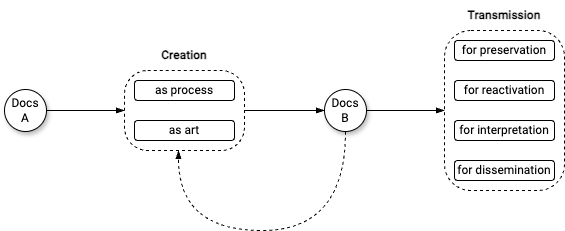
\includegraphics[width=\linewidth]{chapters/2-new_conservation_paradigms/image/graph02-documentation.png}
    \caption{Documentation functions in different stages of the artwork life cycle.}
    \label{fig:c2-documentation}
\end{figure}
Considering the figure, a first distinction has to be made between the \textit{documentation used in the artwork} (\textit{Docs A}) and the \textit{documentation produced from the artwork} (\textit{Docs B}).\\
The first type of documentation (\textit{Docs A}) refers to documents used in the creative process of the artwork. Documentation can be used as a tool for making decisions about the nature and the development of the artwork (documentation \textit{as process}) \cite{dekker2018collecting}. A practical example of documentation \textit{as process} is the work carried out by the media artists group Blast Theory, which used a series of questionnaires, interviews and exercises aimed at the group members themselves and people outside the project to guide the development of the game \textit{Uncle Roy} \footnote{More details about the art project can be found in the Blast Theory website at the link \url{https://www.blasttheory.co.uk/projects/uncle-roy-all-around-you/} (last accessed: 20/09/2024).}\cite{dekker2018collecting}. Documentation can also function as art itself (documentation \textit{as art}). Documentation can refer to a photo, a video, a painting, and other media used to document something and presented in art spaces and through different art forms (e.g. installation). 
\begin{quote}
    Documentation as art means “to use artistic media within art spaces to refer to life itself, that is, to pure activity, to pure practice, to an artistic life, as it were, without presenting it directly.” \cite{groys2008art}. 
\end{quote}
The \textit{Life Sharing} project (2002-2003) of the media art duo 0100101110101101.org is a practical example of documentation \textit{as art}. For three years (from 2000 to 2003), the art group made all of their computer content, such as files, emails and account statements, fully accessible to the public, who could read, download and copy it in real time\footnote{More detail about the art project can be found in the website Net Art Anthology at the link \url{https://anthology.rhizome.org/life-sharing} (last accessed: 20/09/2024).}.\\
The second type of documentation (\textit{Docs B}) refers to documents created during the life cycle of the artwork, whose function extends beyond the deactivation and serves for the interpretation, conservation, reactivation and dissemination and, in general, for the transmission of the artwork toward the future. \textit{Docs B} refer to what is left from the artwork, similar to the performance’s residual objects, which are ``\textit{created in the course of making the performance and during repeated performances}'' \cite{holling2016aesthetics} and once the performance ends, they are the only things left behind, holding memories that can unfold in the present \cite{brignone2009so}. Since the ephemeral nature of live media art, this documentation is the only material that allows for studying, interpreting and reinterpreting an artwork (documentation \textit{for interpretation}). Documentation reflects the understanding of artworks and artistic activities in relation to current and past social and aesthetic values and significance \cite{heydenreich2011documentation:ch7}. It allows for capturing a range of parameters that define the artworks as such, which are crucial for conserving them for posterity \cite{giannachi2022use}. Indeed, documentation is fundamental for conserving the artwork (documentation \textit{for preservation}). 
\begin{quote}
“Documentation provides a tool for monitoring, assisting conservation management and guiding the process of conservation and restoration treatments” \cite{heydenreich2011documentation:ch7}.     
\end{quote}
By interpreting the artwork, we gain insight into what needs to be conserved and the best methods to preserve it, assessing potential risks and ideal conditions \cite{heydenreich2011documentation:ch7}. Consequently, by conserving the artwork, we gain information on how to reactivate it (documentation \textit{for reactivation}). Since it is deactivated, the conservation must consider a new reactivation. Conservation and reactivation can happen through different strategies (like emulation, migration, and virtualisation), but the right approach can only be chosen based on proper documentation. Documentation is generally a tool for communicating and informing about ephemeral artworks across current and future audiences (documentation \textit{for dissemination}).\\ 
However, the documentation that comes from the artwork (\textit{Docs B}) should be understood as something other than merely records or remnants, with only the aim of conserving and presenting the past. Indeed, such documentation should be considered future-oriented \cite{dekker2022documentation, giannachi2022use}. The documentation is not only a derivative of the artwork but also a source for reinterpreting the same work or creating new ones. 
\begin{quote}
“In this sense documentation not only future-proofs but also relentlessly (re-)invents and so (re-)becomes the artwork” \cite{dekker2022documentation}.     
\end{quote}
The installation \textit{Quadrille} by Rose English at Tate is a clear example of an artwork transformed through its documentation over time. The current installation represents the latest stage in the artwork’s evolution. Initially exhibited as an installation in 1974, it was later reimagined as a performance in 1975, incorporating elements from the 1974 installation. Today, it returned to being an installation, this time incorporating costumes, photographs, and videos from the 1975 performance\footnote{Further information about the artwork cna be found in \url{https://www.tate.org.uk/life-artwork-quadrille-rose-english} (last accessed, 4/12/2024)}. Another example is \textit{Il tempo consuma} (1978) by Michele Sambin (a case study carried out by this thesis project\footnote{Please refer to the Appendix~\ref{ax:a-michele_sambin_videoloop} for further information about the case study.}), in which the artist reuses the audiovisual documentation of the first performance inside the digital-reactivated performance or reinterprets the interactive video performance as a static video installation. However, documentation can also serve as a source for creating new artwork. Some examples are the \textit{Reenactments} (2007-2010) of historical performances made by the already mentioned art duo 0100101110101101.org. Instead of simply re-showing and presenting the documentation produced by the original performances (photos and videos), they recreated and performed them inside the video game Second Life, creating a series of new artworks. The duo performed live \textit{Reenactments}, recorded them, and installed them in different formats\footnote{ The performances reenacted are \textit{Seedbed} by Vito Acconci, \textit{Imponderabilia} by Marina Abramovic and Ulay, \textit{The Singing Sculpture} by Gilbert \& George, \textit{Shoot} by Chris Burden, and \textit{Tapp und Tastkino} by Valie Export and Peter Weibel. Some of the video recorded can be found in the duo’s website at the link \url{https://0100101110101101.org/reenactments/} (last accessed: 20/09/2024).}.\\
The live media art documentation process is an accumulation of information, or, as named by Hanna Hölling, a \textit{stratigraphy of documentation} that ``\textit{may never cease to expand, continually depositing new layers on the already accumulated sediment}'' \cite{holling2016aesthetics}. Therefore, in a later article Hanna Höllings proposes to see the work as an archive that is not only a repository of documents but also an ``\textit{intangible, non-physical realm of tacit knowledge and memory in an ever-enduring state of organisation and expansion,}" \cite{holling2017paik} a dynamic entity from which the artworks are actualised and to which they contribute \cite{van2024conservation}.

%%%%%%%%%%%%%%%%%%%%%%%%%%%%%%%%%%%%%%%%%%%%%%
%%%%%%%%%%%%%%%%%%%%%%%% AUTHENTICITY IDENTITY
%%%%%%%%%%%%%%%%%%%%%%%%%%%%%%%%%%%%%%%%%%%%%%
\section{From fixed authenticity to forming identities}
The ephemeral nature of live art and the dynamicity with which documentation is created, accumulated, and used according to artworks raise many questions about authenticity. Questions, discussions, and debates around this concept are born and continue to rise in conjunction with the growing conservation and restoration practices and the establishment of new artistic forms. As briefly mentioned in the previous chapter, live media art proposes a new perspective from which to define authenticity compared with traditional art forms. For this reason, the speculative process around this artistic field has been and continues to be highly heated.\\
In the conservation and restoration context, the concept of authenticity began to be established in the 19th century, especially after the second-post world. The term was bound to the preservation of physical and material aspects of an artwork. Among the most important texts to affirm such an idea are the \textit{Theory of Restoration} (1963) by Cesare Brandi \cite{Brandi2005theory} and the \textit{International Charter for the Conservation and Restoration of Monuments and Sites} (1964) \cite{venicecharter1964} drafted by UNESCO’s \textit{Second Interaction Congress of Architects and Technicians of Historic Monuments}. Both texts refer to the authenticity of art forms such as sculpture, architecture and painting. These artworks are considered to have original ``state'' or ``condition,'' which are identified and revealed in the material and physical evidence. The material and physical evidence can be authenticated, i.e., allowing the identity of an artwork to be defined as a product derived from a human creative process belonging to an author to whom it has been attributed. Therefore, authenticity is used to identify the artwork’s truthiness, ``\textit{and it is often contrasted with the concept of false or fake}'' \cite{jokilehto2010conservation}.
\begin{quote}
    “On the other hand, taking the contrary, i.e. something inauthentic or fake, this can be defined as an artefact where the sources of information have been altered or falsified” \cite{jokilehto2010conservation}.
\end{quote}
The restoration aims to reveal a work of art’s truthfulness; the conservation aims to maintain its integrity. 
\begin{quote}
    “For the majority of traditional art objects, minimising change to the physical work means minimising loss, where loss is understood as compromising the (physical) integrity of a unique object” \cite{laurenson2006authenticity}.
\end{quote}
Another important text was \textit{The Nara Document on Authenticity} (1994) \cite{naradocument1994}, drafted during a World Cultural Heritage conference in Japan in 1994. In this text, the connection between authenticity and materiality began to unbuckle since the concept of intangible heritage was introduced in the speculative process.\\
Summarising this text and the previous important ones, Jukka Jokilehto generally lists three essential parameters with which to define authenticity up to that time \cite{jokilehto2010conservation}:
\begin{itemize}
    \item \textit{Qualitative judgement} about a work is considered a result of the human creative process and, therefore, autonomous and not a copy;
    \item \textit{Legal verification} about the material truth of an object as a historic document;
    \item \textit{Social-cultural traditions} and inculcation of value judgements.
\end{itemize}
These parameters, especially the link between authenticity and materiality, are wholly blurred in the context of live media art. This art form needs new and specific parameters to consider authenticity and thus conserve the artwork.\\
\begin{quote}
    “If the ontological framework is focused on the material so will the notion of authenticity. If the ontological framework shifts, then we expect a similar shift in our concepts of authenticity, change and loss” \cite{laurenson2006authenticity}.
\end{quote}
In his writings, Pip Laurenson \cite{laurenson2004management, laurenson2006authenticity} introduces two essential philosophical concepts that underpin the speculative debate on the authenticity of live media art. These concepts are the \textit{autographic-allographic distinction} defined in \cite{goodman1968languages} and the \textit{two-stage model} in \cite{davies2001musical}.\\
In Language of Art \cite{goodman1968languages}, Nelson Goodman introduces the \textit{autographic} and \textit{allographic} terms within the authenticity context, aiming to separate two scenarios in artistic creation: the forgeable and non-forgeable arts, the arts such as sculpture and paintings and arts such as music and theatre.
\begin{quote}
    “Let us speak of a work of art as autographic if and only if the distinction between original and forgery of it is significant; or better, if and only if even the most exact duplication of it does not thereby count as genuine. If a work of art is autographic, we may also call that art autographic. Thus painting is autographic, music non-autographic, or allographic. [...] One notable difference between painting and music is that the composer’s work is done when he has written the score, even though the performances are the end-products, while the painter has to finish the picture. No matter how many studies or revisions are made in either case, painting is in this sense a one-stage and music a two-stage art.” \cite{goodman1968languages}
\end{quote}
Autographic refers to art where the physical, original object matters. If one attempts to create an exact duplicate of the work, it would be considered a forgery, not an original. Its opposite, the allographic, is an art where the work’s identity is not tied to any particular physical object but rather to a set of instructions or a notation system. Copies or reproductions of these works can still be considered authentic as long as they follow the original notation or instructions.
\begin{quote}
    “In sum, an established art becomes allographic only when the classification of objects or events into works is legitimately projected from an antecedent classification and is fully defined, independently of history of production, in terms of a notational system. Both authority and means are required; a suitable antecedent classification provides the one, a suitable notational system the other. Without the means, the authority is unexercised; without the authority, the means are footless.” \cite{goodman1968languages}
\end{quote}
In \textit{Musical Works and Performances: A Philosophical Exploration} \cite{davies2001musical}, Stephen Davies, following the Goodmanian distinction, introduces the \textit{two-stage model}. The model consists of a composition stage (the first stage) in which the music composition is created and written down through a notational system (i.e. through the compilation of the score) and a performance stage (the second stage) through which the musical work is realised. Each performance is a unique interpretation, providing different perspectives of the original work. The resulting interpretation could be more or less aligned with the original composer’s intention, but it is still rooted in the compositional framework established in the first stage. This model acknowledges that while a score represents the idealised work, each performance contributes to the work’s identity.\\
Pip Laurenson places live media art ``\textit{on the ontological continuum somewhere between performance and sculpture},'' defining it as allographic since it is ``\textit{similar to works that are performed}'' and therefore belongs to those artworks ``\textit{created in a two-stage process}'' \cite{laurenson2006authenticity}. In this context, as required by both the allographic concept and the \textit{two-stage model}, live media art demands a score, better described as \textit{work-defined properties}, usually provided by the artist.\\
\textit{Score compliance} (Castriota, 2024) is essential for defining authenticity in live media art. In this context, the ``score’’ is not an entirely accurate analogy because, due to the diversity of art and related terminological issues, creating a general notation system is unattainable. The score in live media art refers to all the residual documentation (previously called \textit{Docs B}), which helps establish the artwork's \textit{textual stabilisation} \cite{holling2016aesthetics} or, as already mentioned, all the \textit{work-defined properties} in written form. These aren’t just scores (borrowed from the musical context to describe the graphic representation of performance events in space and time) but also instructions, scripts, testimonies, etc. In the absence of the original object, the documentation defines and builds the artwork's identity. Documentation is essential to guide new versions of the artwork, which would be more or less authentic.\\
So, while in autographic art, the parameters of change and loss are discussed according to material and physical authenticity, in allographic art, the idea used to consider the parameters of acceptable change is identity \cite{laurenson2006authenticity}.\\
Moreover, while in traditional conservation, we consider authenticity based on the original state of an object's creation, in live media art, as highlighted by the new documentation's role previously discussed (and shown in Figure 1), we cannot define a fixed but rather \textit{variable} \cite{groys2008art}, or better yet, \textit{under construction} \cite{dekker2022documentation} or \textit{forming} (Phillips, 2015) identity.
\begin{quote}
    "it was recommended that changes in an artwork should be tracked by iterative documentation. In recognising that artworks change, the use of the term ‘original’ started to be avoided, in that it had become clear that it is often impossible to tell which version of an artwork may be the ‘original’ or whether one could even still talk of originals, suggesting, perhaps, that there may not be any difference between various versions of a work". \cite{giannachi2022use}
\end{quote}
Joanna Phillips’ \textit{Documentation Model for Time-Based Media Art} illustrates the idea of forming identity, which establishes a clear distinction between the artwork’s score and its manifestations. All the elements (documentation) that define the work's identity are grouped within the score, while the manifestations represent various interpretations of that score. Although this model resembles Davies’ \textit{two-stage} model, it is an extension. Phillips emphasises that when an artwork enters a collection (or after its first manifestation), it enters a ``state of infancy,'' and its various manifestations contribute to the process of ``forming its identity'' \cite{phillips2012shifting, phillips2015reporting}. This perspective shifts the relationship between identity and authenticity from a unidirectional one to a more bidirectional dynamic.\\
The idea of fixed, original authenticity is replaced by an identity shaped through the different versions or manifestations of the artwork. In Figure~\ref{fig:c2-authenticity}, we summarise the relationship between concepts of authenticity and identity in various art forms. In autographic art, the identity is inscribed inside the authenticity, which can be found in the artwork's original state, which can be restored and preserved. The allographic art’s identity is fixed in a score and informed through different performances of such a score, which can be more or less authentic. Here, we can introduce the concept of dynamic authenticity introduced by Perla Innocenti \cite{innocenti2012bridging, innocenti2012rethinking} to describe the authenticity of performances and non-physical art. Live media art, while often categorised as allographic, surpasses this definition. The artwork's identity evolves as documentation accumulates—encompassing a wide range of materials beyond just a musical score. Therefore, live media art combines the concept of dynamic authenticity with the notion of an identity that is continually forming. Pip Laurenson refers to live media art with the idea of ``epistemic objects'', i.e. objects that are open, incomplete, and whose significances continually emerge through their indefinite ``unfolding'' \cite{laurenson2016practices}. Castriota extends the concept of forming identities by questioning the concept of \textit{centring} in the identity construction of an artwork\footnote{Introduced by Castriota in \cite{castriota2018centres} as the process of drawing hard lines around an artwork’s essential properties.}, introducing the idea of a \textit{multiple perspectives identity} and \textit{multiple centres} \cite{castriota2019authenticity, castriota2024enfolding}.
\begin{figure}[!h]
    \centering
    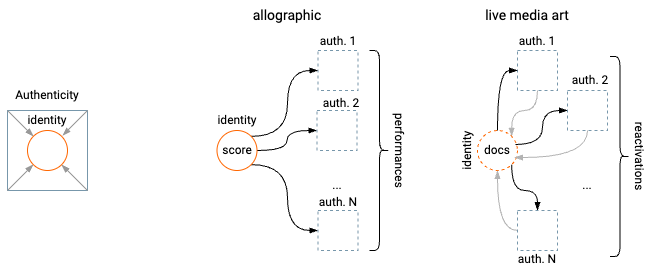
\includegraphics[width=\linewidth]{chapters/2-new_conservation_paradigms/image/graph02-identity.png}
    \caption{Three different models which show the different relation between authenticity and identity in autographic, allographic, and live media art.}
    \label{fig:c2-authenticity}
\end{figure}

\section{The conservation loop}
If the concepts of authenticity and identity change, the activities related to these concepts, such as conservation, preservation, and restoration, also change. Like authenticity, these terms lack an absolute definition. They have been used differently throughout history and across different fields. To resolve this confusion –at least within this text–we will use the definitions of conservation, preservation, and restoration as defined in the context of the essay \textit{Contemporary Theory of Conservation} by Salvador Muñoz Viñas (2005), often used as a reference in literature \cite{munoz2005contemporary}. The author does not define these activities with the goal of fixing absolute meanings but rather as a reference within his book.\\
Muñoz Viñas uses the term ``conservation'' in a broad sense, as the sum of activities aimed at keeping an artwork as it is, plus activities intended to restore the artwork to an ``original nature'' or ``previous version.'' Therefore, this term is considered to encompass both preservation and restoration activities. Preservation can be defined as an activity intended to keep something as it is, maintaining its integrity and thus avoiding alterations and minimising deterioration, with the goal of extending the life expectancy of cultural heritage. However, in reality, preservation involves an intervention in the object, which means it cannot happen without some alteration. The author notes, ``\textit{[p]reservation could thus be defined as the action intended to keep the perceivable features of an object in the present state for as long as possible – a goal which is usually achieved by modifying some of the object's non-perceivable features}.'' Among the different definitions mentioned in the book, for which the author highlights some inaccuracies, he uses the definition of restoration given by the Museum and Galleries Commission, which defines it as ``\textit{all action taken to modify the existing materials and structure of cultural property to represent a known earlier state}" \cite{mgc1994}. Therefore, in contrast to preservation, the author states that ``\textit{restoration can be defined as the action that attempts to modify an object's perceivable features}'' in order to return the object to an earlier state.\\
Restoration and preservation are activities primarily focused on an artwork's present and past states, particularly when referring to physical objects. In the context of live media art, however, the focus of conservation shifts to the experience. For this reason, strategies like storage, migration, emulation, and re-interpretation are proposed as contemporary preservation methods. Since the object of preservation is the experience created by the artwork, these interventions can be considered non-perceivable and evaluated based on a degree of authenticity, much like in musical performances. Interventions on software and hardware (such as migrations and porting) are considered non-perceivable (depending on the specific artwork) since they are part of an assembly that activates the experience, which is the perceivable element.\\
However, the concept of preservation and restoration makes sense when applied to a physical, material object, but it becomes weak when applied to an experience. The experience of an artwork cannot be preserved; Again, it can only be documented. The experience is not only created by the assembly and activation of hardware and software components but, more importantly, by the viewers. Socio-cultural factors shape a person's experience of a work of art or technology. Therefore, when reactivating a live media artwork, it is difficult to talk about maintaining a specific ``state'' or ``condition,'' whether present or past. Instead, supporting the discussion of authenticity mentioned earlier, each reactivation always generates a new experience.\\
Consider \textit{Hole in Space} by Kit Galloway and Sherrie Rabinowitz, a telecommunication art installation that connected people in real-time between two distant locations—Los Angeles and New York City. In the 1980s, this real-time connection across these two cities, several kilometres apart, created a truly impressive, almost science fiction-like experience, perfectly reflecting the installation’s title. However, in today’s world, where real-time global communication is a daily norm, a direct reactivation of the artwork would not evoke the same impact. Recognising this, in 2023, MoMA chose to reactivate the work using a reinterpretation approach. Instead of replicating the original setup, the reactivation relied on documentation from the 1980s to reimagine the experience\footnote{More details about the artwork can be found in the MoMa website, at the link \url{https://www.moma.org/collection/works/120330} (last accessed 13/12/2024).}.\\
This preservation aspect also arose during a case study conducted during this project thesis, specifically in the reactivation and presentation of \textit{Caos delle Sfere} by Carlo De Pirro\footnote{More details about the case study can be found in Appendix~\ref{ax:b-hybrid_reactivation_il_caos_delle_sfere}.}. \textit{Il caos delle Sfere} is a sound installation from 1999 based on an interactive system involving a pinball machine and a Disklavier, which communicate through a computer with dedicated software. The reactivation raised interesting considerations, mainly due to the presence of the pinball machine. In 1999, when the artwork was first presented, pinball machines were common and could be found in many public spaces. The pinball machine has almost entirely disappeared today, resulting in an entirely different impact. For older people, it is a memory; for younger generations, it is a ``novelty.'' As a result, the focus shifted entirely from the interaction between the game and the music to the pinball machine as a historical device, completely altering the experience of the artwork.\\
Therefore, if we consider the experience of the artwork as the ``object'' of conservation, the conservation process itself needs to be redefined. Whether there is a preservation intervention (like migration or emulation), a re-interpretation, or an extremely faithful restoration, the artwork (or experience) will always change. This change is part of what we discussed earlier—the process of forming and shaping the artwork’s identity.\\
Conservation, whether in traditional, autographic, allographic, or live media art, is always about identifying the artwork or, more accurately, defining its identity. In traditional art, conservation assumes that the identity, tied to the artwork’s authenticity, is either revealed (through restoration) or maintained (through preservation). In live media art, however, conservation involves constructing or shaping the artwork’s identity by keeping the essential elements alive so the work can continue to unfold.
In this context, the concept of ``safeguarding'' (Blutter, 2018; Castriota, 2019) is introduced as the opposite of preservation:
\begin{quote}
    "Preserving seeks to secure the life that already is; safeguarding secures and reproduces the conditions of becoming, of living, of futurity, where the content of that life, that living, can be neither prescribed nor predicted and where self-determination emerges as a possibility." \cite{butler2018my} 
\end{quote}
So, while preservation is an activity aimed at fixing the state of something to pass it on to the future, safeguarding aims to maintain the necessary conditions for something to continue to exist (without necessarily being aware of how it will change in the future) \cite{castriota2019authenticity}. Rebecca Gordon names that ``something'' \textit{critical mass}: ``\textit{the optimum choice and grouping of factors or attributes that demonstrate the core identity of the work of art}'' without which the work could not continue to exist \cite{gordon2014identifying}.
\begin{quote}
"safeguarding aims to simply secure the conditions for its future to remain a possibility, a future wherein its identity may evolve, diverge, or multiply." \cite{castriota2019authenticity}
\end{quote}
Therefore, the new concept of conservation–as the action of safeguarding– can be established in a loop between documentation—everything that remains of the artwork after its deactivation, which ensures its survival—and reactivation, which is the transcription and transmission of the artwork that occurs through various methods, always starting from the documentation. This relation between documentation and reactivation is a loop because each reactivation shapes the artwork’s identity and creates new conditions for survival that need to be documented. Figure~\ref{fig:c3-conservation} summarise the differences between traditional and live media art conservation.
\begin{figure}[!h]
    \centering
    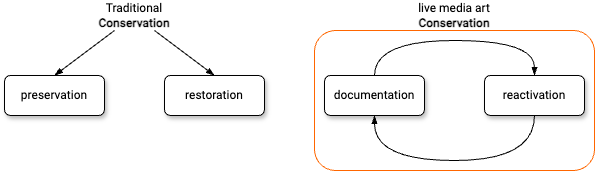
\includegraphics[width=\linewidth]{chapters/2-new_conservation_paradigms/image/graph02-conservation.png}
    \caption{Traditional and live media art conservation paradigms.}
    \label{fig:c3-conservation}
\end{figure}

\section{Reactivation: transcription and transmission}
The term reactivation definitely deserves further exploration, as it is not very common in the literature (though it has been used more frequently in recent years). When used, it is often unclear or confused with terms like \textit{reenactment}, \textit{reconstruction}, \textit{reinterpretation}, and \textit{replication}. As highlighted by Auslander in \textit{Reactivation: Essay on Performances and its Documentation} (2019), the use of this term dates back almost a century \cite{auslander2018reactivations}. It appears in one of the most important contemporary art texts, \textit{The Work of Art in the Age of Mechanical Reproduction} by Walter Benjamin, written in 1935 \cite{benjamin1935work}. In his essay, Auslander introduces Benjamin's concept of reactivation, using Benjamin's own words, such as:
\begin{quote}
    “Technical reproduction can put the copy of the original into situations which would be out of reach for the original itself. Above all, it enables the original to meet the beholder halfway, be it in the form of a photograph or a phonograph record. The cathedral leaves its locale to be received in the studio of a lover of art; the choral production, performed in an auditorium or in the open air, resounds in the drawing room [...] the technique of reproduction detaches the reproduced object from the domain of tradition. By making many reproductions it substitutes a plurality of copies for a unique existence. And in permitting the reproduction to meet the beholder or listener in his own particular situation, it reactivates the object reproduced." \cite{benjamin1935work}
\end{quote}
Benjamin's essay is well-known for its concept of ``aura'' in the context of technical reproduction. The technical reproduction of an artwork deactivates the original, removing it from its historical and local context, thereby stripping it of its authenticity and authority. As a result, technical reproduction takes away the ``aura'' of the original. However, in the excerpt just mentioned, Benjamin also introduces the concept of reactivation, which, as Auslander points out, is often overlooked in the analysis of this famous essay. Technical reproduction does not return the artwork to its original time and space; rather, it places it in a new and current moment and space of experience. Each time the reproduction is ``observed,'' the original artwork is reactivated as a production in the present, not as a replica of a historical past. Therefore, when reactivated through interaction with an observer, reproduction functions as a \textit{post-auretic object} \cite{auslander2018reactivations}.\\
Although slightly different, the writings of Nelson Goodman \cite{goodman1982implementation, goodman1998art} include the terms \textit{activation} and \textit{implementation}, which are very useful for analysing the concept of reactivation in live media art. Both terms refer to all the actions, usually carried out by curatorial projects, that maximise ``\textit{the functioning of the work as a work of art and as that particular work - that is, bringing about insight into and understanding the work}” \cite{goodman1982implementation}. Many activities fall under this umbrella, such as the placement of light, the juxtaposition of two works, the development and placement of a caption, the creation of an exhibition, the publication of a catalogue, and so on. The examples in the essay \textit{Art in Action} (1998) show how these actions are important from the perspective of live media art and in relation to Benjamin's concepts of reproduction and reactivation. The examples include using light to activate paintings, which connects to another example involving the cleaning and care of the artwork ("\textit{cleaning it and lighting it are here partners in activation}"), as well as the conservation of murals and manuscripts, culminating in activation through reproduction.\\
In the context of activation for conservation, Goodman gives a very interesting example: the interventions at the \textit{Lascaux Caves} in southern France. These caves contain 600 ancient murals, estimated to be around 17,000 years old. After being discovered in 1940, the murals began to deteriorate due to exposure to air and humidity caused by the presence of thousands of visitors each day. As a result, the caves were closed in 1963. A full-scale replica of the cave was created in 1980 to activate this archaeological and artistic space and thus enhance access and understanding of the artwork for a wider audience.\\
Another example of activation, which aligns with Benjamin's concept of reactivation, is reproduction, including ``\textit{photographs, transparencies, slides, illustrations in books, and so on.}`` These are not merely ``\textit{replacements, substitutes, surrogates, or proxies for the original}'' but rather tools through which we can activate a work: ``\textit{laypeople and experts alike know or understand most works of art through reproductions}." Goodman refers to this type of activation as indirect activation, where "{action at a distance, or even posthumous action, is possible}'' \cite{goodman1998art}.\\
In essence, Benjamin views reactivation as the interaction between an observer and the reproduction of a work of art. Using the terms \textit{activation} and \textit{implementation}, Goodman refers to the actions taken (usually by experts, curators, or conservators) that enable access to the artwork, thus allowing interaction with an audience.\\
In the context of live media art, specifically for this text, we want to define reactivation to include both meanings. Reactivation encompasses actions aimed at presenting the deactivated artwork in a new space-time context and its resulting interaction (or observation) by a new audience. Therefore, we can define reactivation as the sum of \textit{transcription} and \textit{transmission}\footnote{Terms already presented in the previous chapter in the context of preservation strategies. Transmission, reinscribing and transmission were proposed by the \textit{Archiv Performativ} project.}. By \textit{transcription}, we mean all actions aimed at providing new access to the deactivated artwork, ranging from ``\textit{historical faithfulness to the ‘original’ in reenactment, through interpretative translation in re-performance, to reformulation or transformation in an artistic work}''. Therefore, the \textit{transcription} can be accomplished through different preservation strategies (storage, emulation, migration, reinterpretation, virtualisation, etc.) and \textit{reinscribe} specific artwork aspects. \textit{Transmission} takes place once the artwork has been implemented and thus meets and interacts with the observer, creating a new experience in the new space-time context.

\section{The ecological turn}
At this point, we should ask ourselves how, through all these reactivations, new transcriptions, and transformations—both in the artwork’s presence and in the resulting experience—we can still perceive the artwork as the same specific artwork. How can we track its identity? We might wonder whether the artwork is still the artist’s work or an interpretation by the conservator. Is it then an interpretation of an interpretation? In its unfolding, its formation, and the decentering of its identity, how does that specific work remain the same?\\
Regarding the traceability of the artwork’s variability, Van De Vall and Hollings introduce the concept of \textit{cultural bibliography} in conservation practices \cite{van2011reflections}. Once the artwork enters the museum or the conservator’s hands, it does not stop or die but continues to grow and evolve, developing its biography.
\begin{quote}
“The central idea of the biographical approach is that the meaning of an object and the effects it has on people and events may change during its existence, due to changes in its physical state, use, and social, cultural and historical context” \cite{van2011reflections}.  
\end{quote}
With this approach, the metaphor of the artwork as a living being can be introduced. A living being with its own history, which we can trace through its biography. Similarly, Van Saaze uses the term \textit{career} to describe the variability of the artwork (as defined also in \cite{becker2006art}) and proposes viewing it through \textit{actor-network theory} (ANT) \cite{van2013installation}. According to ANT, the artwork, like other human and non-human entities, is an \textit{actant}—an entity capable of acting or influencing (and, of course, being influenced by) other entities within a network. Thus, through ANT, the artwork is not given once and for all; instead, it occurs repeatedly as a result of the conservation practice itself. The goal of conservation is to find and analyse the transformations of the actants that have shaped the artwork and to reintroduce them into renewed interactions within a network to continue defining the artwork as that specific piece.\\
We define the network of entities interacting to determine the artwork as the \textit{exhibition ecosystem}, which we define here as a second-level ecosystem. The entities (or actants) that interact with and determine the artwork are drawn from other ecosystems, which we refer to as first-level ecosystems. Here, we identify three main first-level ecosystems: the \textit{media and technology ecosystem}, the \textit{institutional ecosystem}, and the \textit{authorship ecosystem}\footnote{These ecosystems are derived from the definition provided in \cite{rinehart2014re} of three external threats that can endanger the future of a live media artwork: \textit{death by technology}, \textit{death by institution}, and \textit{death by law} (the latter expanded here as the \textit{authorship ecosystem}). As threats, these represent ecosystems with which the artwork must interact.}.\\
The \textit{media and technology ecosystem} includes both human and non-human entities, such as the technologies themselves (devices, software, etc.), the companies and individuals who work with and develop them, and the people who use them. It is one of the primary ecosystems that raises the most significant challenges in the conservation of artworks, as it forms the basis of most works and is characterised by a rapidly accelerating process of becoming. As we saw in the previous chapter, the issue of obsolescence is a central concern for many conservation initiatives. This problem triggers a chain reaction within the network of people with the knowledge and expertise to work with specific technologies \cite{laurenson2013emerging}. It continuously renews the user experience and quickly turns technologies from just a few years ago into antiquate tools (as seen with \textit{Hole in Space} and \textit{Il caos delle sfere}).\\
The \textit{institutional ecosystem} is also defined by human and non-human entities, including the people who manage and work in the institution, the institution’s space, its archive, and its collection (including the artworks). This ecosystem refers to the institutions responsible for collecting and exhibiting the artwork, typically represented by museums but also by other institutions discussed in previous chapters. Each institution has its own approach to collecting, conserving, and displaying artworks. It brings a network of different institutions and individuals to satisfy, as well as other artworks with which the artwork must communicate.
\begin{quote}
“The artwork is entangled with the museum’s repertoire, organizational structures, work division, politics, documentation procedures, and level of engagement” \cite{van2013installation}.    
\end{quote}
Next, we have the \textit{authorship ecosystem}, which mostly comprises human entities and includes a more or less distributed group of people (distributed authorship) with different roles. This ecosystem not only plays a creative role but also provides support, including legal guidance on access and usage rights for the artwork or its components.\\
In addition to these omnipresent ecosystems—though they have different balances in each case—there could be other specific entities from other first-level ecosystems that come into play, depending on the artwork. For example, site-specific works engage a unique \textit{space ecosystem} that becomes essential for their realisation.\\
Entities in interaction within and between these ecosystems are put into further interaction within the second-level \textit{exhibition ecosystem}, where the artwork itself becomes an actant. The \textit{exhibition ecosystem} is created through negotiation between the first-level ecosystems so they can interact in relation to the artwork. This negotiation is made possible and limited by the artwork’s \textit{changeability}, which is both its potential to change \cite{holling2017paik} and the limit beyond which an artwork ceases to be the same \cite{van2023theories}. This negotiation defines the artwork’s transformation or variability. The new conservation paradigms establish the basis for this negotiation so that the transforming and growing artwork can no longer be viewed as a fixed entity but rather as an organism adapting to the transformation of an indirect (second-level) ecosystem, made possible by continuous negotiation.\\
To answer the question posed at the beginning of this section, we propose using what Van De Vall refers to as the \textit{ecological turn} in conservation thinking \cite{van2023theories}. According to this approach, the transformation of the artwork, its development and formation over time, should be understood within the context of its environment—its ecology of interactions between the various entities that define the conditions for the artwork’s existence, persistence, and becoming. The \textit{biography} and \textit{career} of the artwork, as well as its forming identity, cannot be defined except as the result of conservation practices, which determine the artwork’s ecology. Therefore, as Van De Vall asserts, in radical cases, it is the very ecologies that produce the ontologies of the artwork:
\begin{quote}
“Rather than deriving conservation practices from the works’ ontology, these ontologies are considered to be the results of these practices.” \cite{van2023theories}    
\end{quote}

\section{Summary}
In this chapter, we defined the fundamental paradigms of live media art conservation. We explored how the artwork becomes a living organism, an \textit{actant} that interacts with and transforms within the \textit{exhibition ecosystem}—a network of complex, constantly changing entities. The artwork is defined within this network, without which it cannot exist. Therefore, conservation practices here are understood as actions aimed at keeping the artwork alive—negotiating with the involved entities and continuously building the interactions that define the artwork. Conservation, then, is no longer about discovering the artwork’s identity but about constructing it, surpassing both the concepts of \textit{autographic} and \textit{allographic} works. This identity is in formation; it develops, grows, matures, and eventually ages and dies. As we’ve seen, this process happens through a potentially endless loop between \textit{documentation} and \textit{reactivation}. Documentation plays a central role in conservation, taking many forms and serving multiple purposes in relation to the artwork and its life. Only with proper documentation we can consider the reactivation of artworks that cannot be physically conserved. Reactivation is the process by which the artwork is \textit{transcribed} through a new balance of interactions between the involved entities, meaning the work is reconstructed from the \textit{documentation} and transmitted through the exhibition ecosystem to these entities, generating a new spatio-temporal experience and creating a new chapter in the artwork’s \textit{biography}.\\
In other words, the past is no longer the goal of conservation. Instead, the past is a tool that conservators use to create the conditions under which the artwork can continue to exist in the present and future. Therefore, the artwork in its current state is no longer the exclusive result of a single artist but rather a collective contribution formed throughout its lifespan, from its creation through its conservation.
    
    \chapter{\label{ch:3-mdc_model-reactivation_workflow-instruction_template}Multilevel Dynamic Conservation Model, Reactivation Workflow and Instructions Template}
In the previous two chapters, we explored the new conservation practices of live media art from two perspectives: from the practical application and outcomes of initiatives and the theoretical and conceptual framework. We examined the developed models for conservation, identifying their common structural elements, and we saw how, conceptually, they strive to apply and consolidate the new conservation paradigms. However, while we can identify similarities between the new conservation practices (particularly in the artwork's acquisition, identification, and iteration), notable differences also emerge.\\
This issue leads us to ask whether it might be possible to discuss standardisation. Standardising conservation practices would have numerous advantages: enhancing accessibility, interoperability, consistency of descriptions, and the efficiency of the tools and systems used. Additionally, they would benefit conservators, who could receive standardised training through specific programs (such as university courses), thereby improving their overall activities and skills. Artists and their collaborators could also adopt standardised procedures and methodologies, improving the conservation of works within their own archives and facilitating acquisitions by third parties. In other words, standardisation could offer significant advantages for the interaction between the various ecosystems involved in the preservation of live media art.\\
Specific standards have already been developed for museum and archive collections, such as \textit{Collection Management Systems} (CMS), also known as \textit{Information Retrieval Systems}. These systems are thought to be integrated into managing and documenting collections, allowing users to search for documents, information within them, and metadata in the databases and their relational structures \cite{dekker2018collecting}. One of the most commonly used CMS in the context of new documentation models is the \textit{Open Archive Information System} (OAIS), which provides guidelines for how archives should acquire, preserve, and ensure the accessibility of digital data over time. OAIS outlines the roles of both the archive and its users, focusing on making preserved information understandable and usable in the future, even if the original technologies become obsolete. However, OAIS and other CMSs are designed to preserve digital data, not specifically for conserving live media artworks. These systems can be integrated into new conservation practices but were not developed specifically for it. On the contrary, live media art conservation models should define how to document, collect, organise, and conserve a work, considering its different components \cite{dekker2018collecting}. Despite numerous attempts, live media art conservation models fail to function as practical standards, often only accepted within the museums or organisations that developed them.\\
\begin{quote}
    "Despite numerous initiatives undertaken during the last two decades, the notion and organisation of artwork-related documentation in museums that collect contemporary art remains neither standardised nor fixed, and, moreover, it is currently facing major challenges" \cite{wielocha2024collections}
\end{quote}
There are many reasons for this lack of standardisation, including the nature of the art itself, the use of cutting-edge technologies and presentation formats, always unique and hard to uniform. Therefore, models developed by institutions are still in their infancy in comparison to the complexity of the art and thus still heavily depend on the museum’s history, subject, scale, and structure \cite{wielocha2024collections}. Moreover, the absence of standardisation stems from the practice of conservation itself, in which the concepts of authenticity and identity that should form the basis of these models are still in development, far from reaching a fully defined, consolidated, and, especially, shared state. Therefore, it may not yet be the time to talk about standardisation—and perhaps it never will be. In this context, the best approach may be to remain heterogeneous and flexible.\\
Given this, we propose addressing the issue from a different perspective, moving beyond the idea of a fixed model or standard and instead using the concept of a meta-model to represent conservation practices. The concept of a meta-model, which emerged in the late 1980s, is now used in various scientific fields, such as mathematics, electronics, and computer science. Suppose we define a model as an abstraction of a real phenomenon. In that case, the meta-model is another abstraction that describes the properties of one or more models—similar to how metadata describes data.
\begin{quote}
“A metamodel is also a model, but its universe of discourse is a set of models, namely those models that are of interest to the creator of the metamodel” \cite{Liu2009-od}.    
\end{quote}
However, our specific application of the meta-model differs from the more commonly used ones in computer science. In our research, we define the meta-model as a set of abstractions from the models introduced in Chapter~\ref{ch:1-state_of_the_art} and the conservation paradigms in Chapter~\ref{ch:2-new_conservation_paradigms}. Its purpose is to present the properties of a \textit{Creative Work} (artworks, artefacts, projects, etc.) in the context of its conservation. This meta-model serves as a general framework for understanding conservation and can be used to design practical models for preservation, documentation and archiving.\\
In environments like museums, with a team of conservators, such a meta-model can be used to structure a specific model and include details inherent to the institution, such as administrative rules, systems to improve communication with the internal archive, and so on. However, the meta-model can also be applied in smaller contexts, such as organising an artist’s personal computer folders or structuring the repository of an artistic project. Sharing the same organisational structure at a higher (meta) level could make the acquisition process more accessible to museums. A meta-model take into account the network of entities related to the creative works and their relation, promoting a controlled multiplicity of applications. This means having several applications that follow a set of guidelines and can marge into the properties used.\\
So, while we may not achieve full standardisation benefits, a meta-model can simplify the sharing and accessibility of documentation and conservation processes.\\
The meta-model presented in this chapter is the \textit{Multilevel Dynamic Conservation} (MDC) model, developed from the representation of an artwork as a multi-typological archive and as an extension of a model created between 2009 and 2014 at the Centro di Sonologia Computazionale (CSC) at the University of Padua for musical installations. This meta-model is designed to define administrative models for archiving and conserving creative works and their related heterogeneous components and documentation. This chapter will also introduce two other essential tools that can be paired with the MDC model: a workflow for the reactivation process called CATTA (\textit{Collection}, \textit{Assessment}, \textit{Transcription}, \textit{Transmission}, and \textit{Archiving}) and a template for the compilation of the artworks' technical instructions. The latter, developed from the instructions used in electronic music scores, also incorporates the adaptation of the Visual Language for describing mappings as defined by Marije Baalman in \cite{baalman2022composing}.\\
All these models summarise the state of the art, considering the most important outcomes of the projects analysed in Chapter~\ref{ch:1-state_of_the_art} and the new conservation paradigms studied in Chapter~\ref{ch:2-new_conservation_paradigms}. The next chapter will demonstrate the MDC model's adaptability across different application contexts. Appendices~\ref{ax:a-michele_sambin_videoloop}, \ref{ax:b-hybrid_reactivation_il_caos_delle_sfere}, \ref{ax:c-the_score_in_live_electronics_music}, and \ref{ax:d-sustainability_and_longevity_of_nimes} will show the CATTA reactivation workflow's applications and the compilation of the instructions.

\section{Multilevel Dynamic Conservation (MDC) Model}
The first version of the \textit{Multilevel Dynamic Conservation} (MDC) Model was developed at the Centro di Sonologia Computazionale (CSC) in 2009 to extend their audio preservation methodology \cite{bressan2016atr, fantozzi2017tape, pretto2019computing}. It was left aside around 2014, but work on the model was revived in January 2021 as part of this PhD research project, with support from both the CSC and Audio Innova Srl\footnote{Audio Innova Srl is a spin-off of the University of Padua, co-founded by Sergio Canazza, who currently serves as both CEO of the company and Director of the CSC. Audio Innova is partner of the PhD research project.}.\\
The CSC is a laboratory at the University of Padua, established in the 1970s, dedicated to research and production in digital sound and computer music \cite{canazza2019four, canazza2022gesture}. Its work ranges from tape music to interactive music installations. Given the large amount of music created on magnetic tapes \cite{pretto2020active}, CSC researchers developed a preservation method specifically for this material, including specific software for supporting the creation of preservation copies of analogue recordings (PSKit) \cite{fantozzi2017tape}. This preservation method is still widely used today by both the CSC and Audio Innova for digitisation projects, not only for their own archives but also for external ones.\\
However, this methodology still proves inadequate for a significant portion of the CSC's artworks. Since the 1990s, CSC production has gone beyond tape music and included multimedia installations and performances. To preserve these more complex works, CSC researchers began expanding their conservation approach to address the challenges of live media art.\\
Between 2009 and 2014, CSC researchers worked on a series of case studies focused on Carlo De Pirro’s installations in a project called CAPIRE (\textit{CArlo De PIrro: Restoring an Experience}). The project led to the creation of a model for preserving and reactivating interactive multimedia art. As an expansion of their audio preservation strategy, this model introduced new methods for preserving all the elements of interactive multimedia art, as well as the experience it creates \cite{bressan2014challenge}.\\
The multilevel model developed by the CSC is a functional categorisation of documents and is an extension of the CIDOC Conceptual Reference Model (CIDOC-CRM), an ISO standard for describing cultural heritage. The model borrows concepts from both audio preservation and computer science. On the one hand, as an extension of the audio preservation methodology, it incorporates the idea of a preservation copy. The preservation copy is an artefact designed to be stored and maintained as the preservation master \cite{miliano1999iasa}. It consists of an organised dataset containing all the information the original document represents, along with metadata and documentation about the preservation process.\\
On the other hand, the model is structured as a multilevel hierarchy based on a framework for preserving scientific data used in computer science. In this context, the multilevel structure includes \textit{bit} (the lowest level of representation), \textit{data} (attributes), \textit{record} (tuples), and \textit{experience} (the knowledge generated by interpreting the data).\\
In the context of artwork preservation, the preservation copy is defined as follows:
\begin{itemize}
    \item \textit{Bit}: Every part of the original artwork that can be directly preserved, including both digital and physical objects. (The preservation of digital objects follows the general conceptual model defined by the OAIS reference model);
    \item \textit{Data}: Technical notes, comments, and relevant information about the creation of the artwork;
    \item \textit{Record}: Any element that has been modified or updated in relation to the original artwork;
    \item \textit{Experience}: Any document that informs about the appearance and overall experience of the artwork.
\end{itemize}
This multilevel model aims to support various ways of exploiting and archiving preserved artwork. This hierarchical structure provides different levels of information with varying degrees of detail and complexity, allowing for historical and philological studies, analysis, reconstructions, replications, and reinterpretations depending on the specific purpose.\\
This model has been applied to various case studies, including those in the CAPIRE project. It was mainly used for Carlo De Pirro’s \textit{Casetta delle Immagini} and \textit{Carillon della Materia} installations. The first is an installation exhibited at the 2002 Expo in Switzerland, which featured a mixed reality environment where cameras tracked participants' gestures to generate sounds, images, and colours. The second is a wooden structure made of carpenter’s tools, transformed into a musical instrument that automatically plays compositions by Carlo De Pirro. Another case study outside of the CAPIRE project was the recreation of Adriano Guarnieri’s video opera \textit{Medea} as a multimedia installation \cite{bressan2009preserving, bressan2014challenge}.\\
The model was tested and refined through these case studies, showing its potential for preserving multimedia and installation art. However, its development and application were halted with the closure of the CAPIRE project.\\
The model has been revisited as part of this PhD research project to update it to the latest live media art conservation developments and give it a more formal structure. Previously, the model lacked a clear structure—for example, it was unclear how all the elements were grouped and related to a work of art, and the relationship between the levels and the contained elements was not well defined. Another aspect that has been revised is the scope of the model. Initially, the model was designed to be applied exclusively in the digital domain. However, aiming to create a meta-model, we broaden its applicability to further include the artwork's physical components\footnote{In the Author’s articles preceding this thesis \cite{fiordelmondo2023toward, fiordelmondo2023multilevel, fiordelmondo2024reactivating, fiordelmondo2024nime}, we name the model \textit{Multilevel Dynamic Preservation} (MDP) using ``preservation'' rather then ``conservation'' as its application was limited to digital contexts. Indeed, we can talk about preserving a set of digital files, but this doesn’t extend to the artwork itself if we align with the new conservation paradigms discussed in the previous chapter. While the term ``preservation'' is commonly used in the literature, we have seen that it no longer makes sense to ``keep something as it is'' in live media art, which embraces concepts of dynamicity and unfolding –at least if we use the Munoz-Vinas’s definition of preservation \cite{munoz2005contemporary}, which is by no means absolute. Instead, when we talk about conservation in this context, we are referring to maintaining the ``\textit{necessary conditions for something to continue to exist}'' \cite{castriota2019authenticity}.}.\\
Building on the prototype structure left in 2014, we have reformulated the multilevel model as a meta-model. This revisitation is based on international projects and models developed for new conservation practices (as mentioned earlier) and designed using the ISAD(G) structure as a reference.

\subsection{The artwork as a multi-typological archive and the ISAD(G) standard}
If we look at the artwork as an aggregate of heterogeneous components and as a \textit{stratigraphy of documentation} \cite{holling2016aesthetics}, we can compare the artwork to an \textit{archive}, as proposed by Hanna Hölling \cite{holling2017paik}, or more precisely, to a ``multi-typological archive.''\\
First, we can define an archive as a collection of documents created or gathered by one or more individuals for a specific purpose. For an archive to exist, it must have an \textit{archival bond} \cite{de1988archivio}—the logical and necessary link connecting the documents—and an \textit{archival context} \cite{pitti2003descrizione}—the circumstances under which the archival documents were created and used. The term ``multi-typological'' or ``expanded'' describes an archive with an \textit{archival bond} and \textit{context}, yet its documents are heterogeneous, often including unusual elements \cite{brunetti2018archivio}. The analogy with an artwork becomes clear: it is multi-typological –with various types of heterogeneous components and documentation–where the \textit{archival bond} and \textit{context} converge in the artwork itself –what links all the pieces is the circumstance of their creation and use, i.e. the artwork.\\
In this analogy between artwork and archive, the ``archival description'' concept is vital. It is one of the most critical archival activities, defining the archival units, documents, and their relationships \cite{brunetti2018archivio}.
\begin{quote}
“[...] describing archives means situating the descriptions of individual entities (such as series, units, documents) within the archival context to which they belong. In other words, it means clarifying and making explicit the relationships that link individual entities (the parts) to each other, to the larger whole, and to the context of document creation” \cite{vitali2000standard}.
\end{quote}
Building on this formulation of the artwork, we introduce the archival description standard developed by the International Council on Archives (ICA): the \textit{General International Standard of Archival Description} (ISAD(G)) \cite{ica1999general}. ISAD(G) proposes a theoretical model for representing archives. The model's hierarchical structure is particularly important in our context, as it allows for a multilevel description, from the general (\textit{fonds}) to the specific (documentary unit), as shown in Figure~\ref{fig:c3-isadg}.
\begin{figure}[!h]
    \centering
    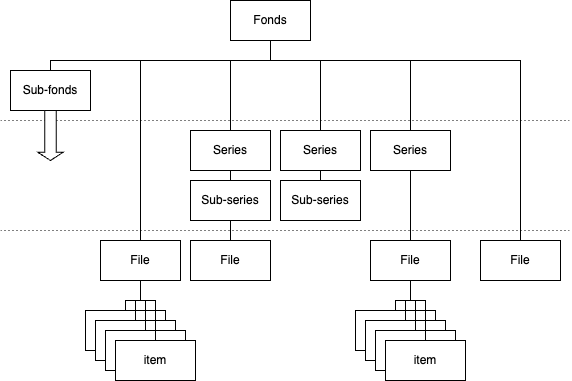
\includegraphics[width=\linewidth]{chapters/3-mdc_model-reactivation_workflow-instruction_template/image/graph03-isadg.png}
    \caption{Graphical representation of the ISAD(G) model’s hierarchical structure.}
    \label{fig:c3-isadg}
\end{figure} 
As outlined in the ISAD(G) text, the hierarchical levels can be described as:
\begin{itemize}
    \item \textit{Fonds}: The whole of the records, regardless of form or medium, organically created and/or accumulated and used by a particular person, family, or corporate body in the course of that creator's activities and functions.
    \item \textit{Series}: Documents arranged in accordance with a filing system or maintained as a unit because they result from the same accumulation or filing process, or the same activity; h
    \item \textit{File}: An organised unit of documents grouped together either for current use by the creator or in the process of archival arrangement, because they relate to the same subject, activity, or transaction. A file is usually the basic unit within a record series.
    \item \textit{Item}: The smallest intellectually indivisible archival unit, e.g., a letter, memorandum, report, photograph, sound recording.
\end{itemize}
The structure is just one perspective of the archival description provided by ISAD(G) (the standard also defines 26 descriptive elements to elaborate on the description of each archival entity). In the context of an artwork, this hierarchical structure is highly relevant, as it can serve as a representation of its related components and documentation. By adopting the ISAD(G) model, we can consider the artwork as an archival \textit{fonds}, within which all related physical or digital pieces are included. Since live media art often consists of one or more \textit{series} of iterations, these iterations can be viewed as archival \textit{files}. Each archival \textit{file} representing an iteration of the artwork contains all the items that belong to that specific iteration. As illustrated in Figure~\ref{fig:c3-isadg_art}, we can use the ISAD(G) hierarchical model to represent the relationships between the artwork.
\begin{figure}[!h]
    \centering
    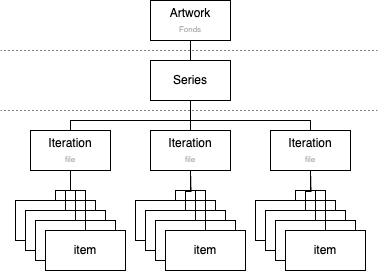
\includegraphics[width=0.7\linewidth]{chapters/3-mdc_model-reactivation_workflow-instruction_template/image/graph03-isadg_art.png}
    \caption{Representation of the artwork as an archive according to the ISAD(G) model’s hierarchical structure.}
    \label{fig:c3-isadg_art}
\end{figure} 
Based on this representation, we could elaborate and formalise the multilevel model developed by the CSC in a more structured way to better represent creative works.

\subsection{Structure}
Figure~\ref{fig:c3-mdc} shows the updated representation of the \textit{Multilevel Dynamic Conservation} (MDC) model. We replaced the diagram structure with a matryoshka-style representation to better illustrate how documentation layers contribute to the artwork's identity.
\begin{figure}[!h]
    \centering
    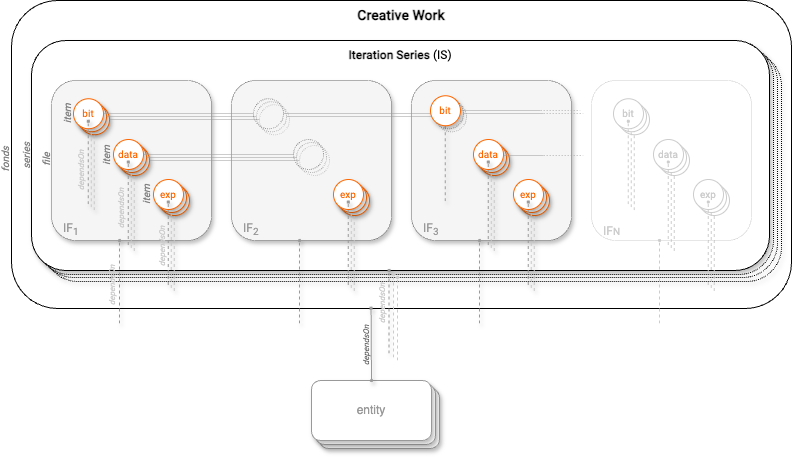
\includegraphics[width=\linewidth]{chapters/3-mdc_model-reactivation_workflow-instruction_template/image/graph03-mdc.png}
    \caption{Graphical representation of the Multilevel Dynamic Conservation (MDC) Model.}
    \label{fig:c3-mdc}
\end{figure} 
The model has three key properties: \textit{multilayering}, \textit{multiple belongingness}, and \textit{dependencies}.\\
Regarding the first property, the model consists of four main levels, arranged hierarchically to move from the general to the specific. The top level represents the \textit{Creative work} itself, which could be an artwork but also an artistic project or artefact. Like a \textit{fonds}, it includes all related items. The \textit{Creative work} consists of an \textit{Iterations Series} (IS), which contains all the manifestations or versions of the artwork. Typically, a creative work has one IS, but multiple \textit{Iteration Series} can be created in exceptional cases or based on archival needs. Other series types can also be included. For instance, if there are pieces of information unrelated to any specific manifestation but to the creative work as a whole (such as bibliographic references or analysis of an artwork), a dedicated series (like a \textit{Bibliography Series}) can be created. However, only the main IS is mandatory. The IS contains individual iterations called \textit{Iteration Files} (IF). An IF is essentially a container—or folder, in analogy to the ISAD(G) framework—that holds all the items associated with a particular iteration of the work. The lowest level represents the individual items of a work's manifestation (iteration or version). These items are the physical and digital elements that form the artwork, such as the components, instructions, scores or any other documentation that captures the experience of each version. At this level, we can reintroduce the division from the first version of the model. The items within each IF can be grouped into three distinct types:
\begin{itemize}
    \item \textit{Bit}: These are all the physical and digital parts that make up the work, such as hardware, software, installation and performance objects, and fixed-media files (e.g., video or audio components used in the manifestation). 
    \item \textit{Data}: This refers to all the information necessary for realising the work. These elements form the work's instructions, mappings, or scores, particularly regarding how the components (\textit{bit}s) should be linked, used, activated, and arranged in space and time. Examples include operating instructions, musical scores, scripts, technical notes, comments on the work, and high-level descriptions of algorithms and models.
    \item \textit{Experience}: This includes documents that capture the work's experience, such as interviews, audio/video recordings, and usability tests of the original system. It also covers information about the people involved in the realisation of the work (artists, performers, technicians) and their roles. Additionally, any documentation related to the reactivation or preservation of the work (e.g., descriptions of approaches, methodologies, and software used) falls into this category.
\end{itemize}
While these physical and digital elements are collected separately, they should be seen as closely connected and following, even in this case, a hierarchical information structure, as defined by the original multilevel model. Figure~\ref{fig:c3-items} illustrates the artwork's hierarchical structure of \textit{bit}, \textit{data}, and \textit{experience}. 
\begin{figure}[!h]
    \centering
    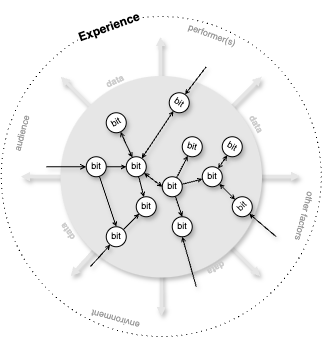
\includegraphics[width=0.7\linewidth]{chapters/3-mdc_model-reactivation_workflow-instruction_template/image/graph03-items.png}
    \caption{The hierarchical structure of bit, data and experience.}
    \label{fig:c3-items}
\end{figure} 
Compared to the previous version of the model, one type of item, the \textit{record}, is no longer necessary. Any modifications to the original artwork are recorded within each \textit{Iteration File}, and the overall changes can be traced by reviewing the \textit{Iteration Series} as a whole.\\
Another essential property of the MDC is the \textit{multiple belongingness}. As we can see in the graphical representation of the model in Figure~\ref{fig:c3-mdc}, \textit{bit} and \textit{data} type items can belong to multiple IFs. If some parts (or even all parts) of the original or previous manifestation are reused in an ongoing reactivation, those will also be registered as elements of the new IF. The \textit{multiple belongingness} of items is an important property of the presented model, which differs from the general structure of the ISAD(G) in which each archival unit (\textit{item}) only belongs to a unique file. The \textit{multiple belongingness} can be applied only to \textit{bit}- or \textit{data}-type items since \textit{experience}-type ones are designed to document the ongoing manifestation. It thus must belong to a unique IF. This property allows the artwork to be represented not as a mere group of delimited records but rather as a process or a dynamic object\footnote{In other words, the experience is the product of the mapping of all \textit{bit} (the \textit{data}) within a specific spatio-temporal context as also shown in Figure~\ref{fig:c3-items}, i.e. it belong to a specific iteration, and can not be the same for other ones}.\\
The same property can be applied at a higher level across different artworks. Items from the \textit{Iteration Series} category (e.g., a software), as well as items from other types of series (e.g., a bibliographic item), can be shared across multiple artworks. Even \textit{experience}-type items can be shared among multiple artworks if the same items document all these multiple artworks. In particular cases, even an entire series can belong to more than one artwork\footnote{Consider the \textit{Reenactments} by the duo 0100101110101101.org mentioned in the previous chapter. Depending on the archival approach, the various presentations (iterations) of the virtualized historical performances can either belong to the specific \textit{Reenactment} by the duo (thus treated as a standalone artwork) or be considered reproductions of the original historical works, performed in a virtual environment, and therefore classified under those original works. The MDC model does not exclude either option, allowing for both interpretations simultaneously.}.\\
The last property of the model is the \textit{dependence} of various levels and items on entities. These dependencies can have different types necessary for applying the model, such as \textit{isOwnedBy}, \textit{isProducedBy}, \textit{isCreatedBy}, \textit{isRealizedBy}, etc. Still, they can also be more specific, such as \textit{isPerformedBy}, \textit{isCuratedBy}, and so on. Entities can also vary depending on the needs, and we can include people, organisations, institutions, companies, etc. Even within the dependency relationships, we can apply \textit{multiple belongingness}, meaning these relationships can be multiple: levels and items can depend on more than one entity, and vice versa, i.e., the same entity can relate to multiple levels or items. This property and \textit{multiple belongingness} allow us to track the artwork's transformation based on the dependency relationships.\\
As a meta-model, the MDC model does not define the metadata structure for digital components or preservation methods for physical ones. Instead, the model states the properties of creative works as a function of their conservation. Informational and practical levels would be defined in constructing an application model. They could refer to existing external standards (e.g., the previously mentioned OAIS reference model for digital items) or requirements of a specific institution.

\section{Reactivation workflow}
Alongside the MDC model, designed to guide the conservation of creative works, we introduce a reactivation workflow to represent the process of reactivating the work with each new iteration.\\
The workflow model was developed in collaboration with the Department of Computational Media and Arts (CMA) at the Hong Kong University of Science and Technology in Guangzhou (HKUST(GZ)), China\footnote{During the PhD research project, a 6-month Visiting Research Program was conducted at HKUST(GZ) with the goal of developing and formalising the reactivation workflow presented here. The 6-month Visiting Research Program was supervised by Assistant Professor Raul Masu.}. The workflow model was initially developed for Digital Musical Instruments (DMIs). While this context differs slightly from live media art, it is still closely related, as it focuses on creating original interfaces for performances, installations, and educational and inclusive applications.\\
In a broad sense, DMIs can be viewed as hardware and software aggregates, consisting of both a controller or gestural interface and a digital sound synthesis method to generate and process sounds in real-time \cite{miranda2006new}. For the development of this workflow, we primarily focused on DMIs developed in the context of the New Interface for Musical Expression (NIME) conference, where new DMIs are presented and implemented in installations and live performances every year\footnote{New Interfaces for Musical Expression website: \url{https://www.nime.org/} (accessed 15/12/2024).}. The conference is based on the usage of new technologies in designing instruments for musical expression, with an increasing focus on audio-visual expression \cite{jensenius2017nime}.\\
However, in recent years, the NIME community has recognised issues surrounding short-term engagement with these instruments, both in terms of reduced artistic use and wasted potential of the devices themselves. A significant problem is that these instruments often fail to be used beyond their initial presentation \cite{mamedes2014nime}. Morreale and McPherson conducted a systematic review of NIME projects \cite{morreale2017nime}, showing that only a small percentage of the devices showcased at the conference have been used in more than one performance. Many research-based DMIs (such as those presented at NIME) often remain as prototypes, abandoned in favour of developing new instruments, compromising both the instruments' mastery and further artistic and expressive experimentation.\\
In response, various studies have examined DMI longevity and sustainability, offering practical guidelines and best practices (e.g., using FLOSS, documenting instruments, employing modular designs, and considering musical outcomes). Despite this, as a recent systematic review \cite{masu2023nime} revealed, among nearly 300 papers published in the 2020–2022 editions of the NIME conference, only 9\% addressed the reuse and repurposing of DMIs, while 67\% introduced new ones\footnote{Notably, this trend does not seem to change: if we consider the proceeding of the NIME 2023, in which only 6 papers deal with the reuse and repurpose of DIM (∼6\% of the 99 papers published).}.\\
In light of this issue and the need for more sustainable solutions, the MDC model has been proposed as a framework for the sustainability and preservation of DMIs. The model was applied in a specific case study: the reactivation of \textit{Soundrise}, an interactive multimedia application for deaf children. A multimedia application is a creative work with challenges similar to live media artworks, such as technology, documentation, interaction, and creative and collaborative processes. However, there is a key difference: for multimedia applications, the evolution of the work is taken for granted, and the final version is the most important (as important as the original in traditional art). Unlike artworks, these applications are not framed within the broad and complex theoretical context of art, and concepts like authenticity and identity are more superficial, often linked to legal matters instead. However, this case study aimed to examine a multimedia application from the perspective of live media art and thus proposing an innovative solution for the sustainability of such creative works. During the application of the MDC model, it became clear that reconstructing an application follows distinct steps, each with specific functions and outcomes. As a result, the study led to the development of a formal workflow to describe the reactivation process.

\subsection{Structure}
\begin{figure}[!h]
    \centering
    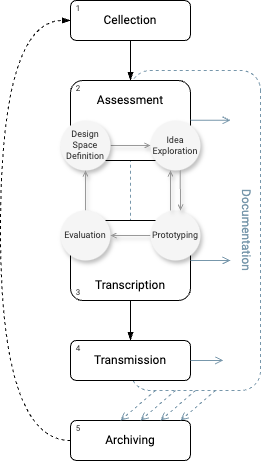
\includegraphics[width=0.7\linewidth]{chapters/3-mdc_model-reactivation_workflow-instruction_template/image/graph03-catta.png}
    \caption{Graphical representation of the CATTA reactivation process.}
    \label{fig:c3-catta}
\end{figure} 

Figure~\ref{fig:c3-catta} shows a graphical representation of the reactivation workflow called CATTA. The CATTA workflow consists of five steps, from which its name is derived: \textit{Collection}, \textit{Assessment}, \textit{Transcription}, \textit{Transmission}, and \textit{Archiving}. These five steps aim to ensure consistent reactivation and facilitate future ones. As shown in the graphical representation, the CATTA workflow also includes sub-steps borrowed from the \textit{design process} introduced by Filipe Calegario in \textit{Designing Digital Musical Instrument Using Probatio} \cite{calegario2018designing}. The design process is not exclusively developed for DMIs; it rather functions as a general description comprehending different areas. It is defined by \textit{Design Space definition}, \textit{Idea exploration}, \textit{Prototyping}, and \textit{Evaluation} steps and helps to better nuance the central CATTA’s \textit{Assessment} and \textit{Transcription} steps.\\
As following, we describe the CARIA process steps:
\begin{enumerate}
    \item \textit{Collection}: The first step involves collecting (or acquiring) all of the creative work's components at every stage of its development, from the first manifestation to the latest. In this step, the acquisition includes all physical and digital parts, scores, instructions, and documents that demonstrate the state of the creative work throughout its iterations. The goal is to collect as much information as possible and to have a clear understanding of its dynamics. At this point, pre-acquisition and acquisition steps (as seen in live media art conservation initiatives) can be included, along with the compilation of the \textit{identity report}. If the MDC model is applied, this is where all the artwork’s elements are organised according to its hierarchical and dynamic structure, defining the creative work level (e.g., through the \textit{identity report}) and the \textit{iteration series} by completing the iteration files and classifying the elements as \textit{bit}, \textit{data}, or \textit{experience}.
    \item \textit{Assessment}: This step involves evaluating any issues, problems, vulnerabilities, and the potential of the previous versions of the work. Condition reports can be created (if not already available), and depending on preservation choices, assessments can be done at the level of the creative work, individual iterations, or both. However, this evaluation does not just focus on past iterations but mainly looks forward to future ones. The CATTA process is used when creative works need to be reactivated, so assessments must not only address weaknesses but also plan for the upcoming reactivation, thus finding the best conditions for the work to continue to exist. Therefore, new parameters for reactivation are necessary to consider, and they depend on various factors like space, the event, performers, etc. In other words, we are now looking at the variables that enable the necessary negotiation among the different ecosystems—essential for conserving the creative work, or more precisely, for ensuring its survival during this reactivation and the next one.\\
    At this point, we include the design process's sub-steps of \textit{Design Space definition} and \textit{Idea exploration}. The \textit{Design Space definition} is ``\textit{related to understanding the concept [of the reactivation], such as the stakeholders, the scenarios, the common knowledge of the area: understanding the user’s interaction and context of use; and defining restrictions that define the designing space of the project}'' \cite{calegario2018designing}. The \textit{Design Space} ``\textit{constraints design possibilities along some dimensions, while leaving others open for creative exploration}" \cite{beaudouin2003prototyping}. In practice, the \textit{Design Space} is defined by the collected elements and the context in which the work will be presented. This sub-step involves not only following the artist's instructions (intentions and constraints) and adapting them to a new context or evaluating the \textit{bit}s (physical and digital components) that may be missing or malfunctioning. It also involves considering the circumstances of the reactivation, such as the event, purpose, and the economic conditions underlying it.\\
    Once these boundaries are defined, the next sub-step is \textit{Idea exploration}, where potential development paths are explored. In this sub-step, we try to expand the \textit{Design Space}, especially in very constrained cases—like when an artwork is site-specific or tied to a particular historical moment. We may also explore technology migration, emulation, or even complete reinterpretations of the work. During this sub-step, a decision-making tool, such as DOCAM’s \textit{Decision Tree}, can be applied to evaluate development paths.\\
    The \textit{Design space definition} and \textit{Idea exploration} sub-steps defined in \cite{calegario2018designing} offer a structured method for determining the creative work’s \textit{changeability}.
    \item \textit{Transcription}: After identifying possible development paths and thus the \textit{changeability}, the \textit{transcription} step aims to create ``prototypes'' of the reactivation, evaluate their effectiveness, and finally produce the concrete reactivation of the creative work.\\
    This step includes two sub-steps: \textit{Prototyping} and \textit{Evaluation}. In \textit{Prototyping}, the reactivation ideas are implemented, focusing on practical and functional aspects. Here, the collected \textit{bit}s are assembled according to the instructions (\textit{data}). New \textit{bit}s may be introduced depending on the development path, so new assembly criteria and instructions must be developed. The prototyping process is not done in one go; it passes through different stages and levels of fidelity, which are evaluated during the \textit{Evaluation} sub-step. \textit{Prototyping} can be experimental, testing different development paths, or exploratory, overlapping with the previous \textit{Idea Exploration} step. Prototypes range from \textit{low-fidelity}—where representations are simple, usually on paper, with limited details and focused on specific aspects (initial prototype)—to \textit{high-fidelity}–where the development path is applied concretely with many details (working prototype). \\
    Each prototype requires evaluation to either continue and improve the prototyping process or to reassess the documentation, returning to the \textit{Assessment}'s \textit{Design Space} definition sub-step to redefine the approach.\\
    During the \textit{transcription} phase, all the activities needed to make the artwork accessible to the public should be considered and developed. They include setting up the artwork in relation to other works, promoting it, creating catalogues, and providing general information.
    \item \textit{Transmission}: After the transcription step, the artwork should be functionally reactivated, meaning it is ``transmitted'' to the audience so they can experience it. The transmission involves the performer(s) and the audience interacting with the work, generating the experience of that specific creative work.
    \item \textit{Archiving}: The final step is archiving the documentation produced during reactivation. This step is crucial for conservation. All the other steps generate a large amount of documentation: condition reports and other evaluations from the \textit{assessment}; all prototypes and evaluations from the \textit{transcription} step (which often produces the most information); and documentation about the setup and, most importantly, the experience of the artwork during the \textit{transmission}. Only by archiving this documentation can future reactivations take place, ensuring the conservation of the creative work.
\end{enumerate}
The separation of steps in the CATTA process is not rigid; the steps do not follow in a strictly discrete order but rather overlap and intertwine. Although the \textit{assessment} step is supposed to begin after all elements of the artwork are collected, these two steps can also occur simultaneously, as each piece of the work can be assessed during the collection phase. Additionally, the \textit{assessment} and \textit{transcription} steps interact closely. During the \textit{transcription}, it is often necessary to return to the \textit{assessment} phase (as described in the design processes’ sub-steps). The \textit{transcription} step can also overlap with the \textit{transmission} step. For example, issues that arise during setup or installation, or new unforeseen behaviours observed when the artwork interacts with the audience, may require reevaluation and adjustments, causing a return to the \textit{transcription} (or even the \textit{assessment}) step. The \textit{archiving} step is the most evident case of overlap, as it should ideally take place alongside the other steps, which are generating documentation, rather than only after all the other steps are completed. Therefore, the steps are more or less simultaneous, and their incremental order is not purely sequential or time-based but rather based on dependencies. For instance, we can conduct an \textit{assessment} if we have some collected documents (even just one), move to \textit{transcription} based on an \textit{assessment}, proceed with \textit{transmission} if we have a functioning work, and finally, \textit{archiving} can only happen if documentation has been produced in the other steps.

\section{Instruction template and Baalman Visual Language}
Finally, we introduce the last system: the \textit{Modular Instruction Framework} (MIF). This system was developed to guide the documentation of the technical information needed to reactivate the artwork—i.e., the \textit{data} level in the MDC model. Referring back to the MDC model’s graphical representation and Figure \ref{fig:c3-items}, which illustrates the hierarchical structure of items, we can see that the \textit{data} level is crucial. The \textit{data} connects all the \textit{bit}s to each other (at the lowest level) and to the \textit{experience} (at the highest level). In simpler terms, the \textit{data} level is like the brain of the work and a key element in its conservation. It consists of the information that defines how all the elements relate to each other across different dimensions (spatial, temporal, processual, gestural, etc.). The \textit{data} largely contributes to determining the work’s identity, meaning that the same group of \textit{bit}s can create two entirely different \textit{experiences} depending on how they are mapped.\\
While we can easily identify a \textit{bit} or a piece of \textit{experience} (like a computer, software, audiovisual file, or photo), defining \textit{data} is less straightforward. How do we concretely describe it? Is it a diagram, a set of instructions, a score, or a combination of these things? Can it be seen as a multimedia file, a fixed digital text, or something on paper? Do we need to follow specific notational systems or standards?\\
In this section, we will clarify the concept of \textit{data} and offer practical solutions for compiling this level.\\
The \textit{data} level contains all the information on how to set up and run the work, including instructions, musical scores, high-level descriptions of algorithms, and so on. In other words, it includes information on \textit{bit}s and their interaction, including the interaction with external agents such as the environment, performers, audiences, and other factors. Unlike the usual comparison with a score, here we introduce the term \textit{mapping} to group all these types of ``information'' —a term typically used in the field of interaction design. Mapping is essential for describing the artwork because it captures the core elements ``\textit{where the artist expresses themselves}'' \cite{baalman2022composing}. As Marije Baalman states, ``\textit{The question of mapping is central to creating artistic meaning in interactive, digital art}'' \cite{baalman2022composing}. Mapping can be seen as the invisible part \cite{delahunta2001invisibility} of interactive work, the element that connects gestures (of any kind, from a controlled action by a performer to an uncontrolled action by a non-human actor, i.e., any physical phenomenon that changes over time) with specific outputs (lights, sounds, videos, heat, robot movements, fan-generated wind, vibrations, etc.). Here, however, we use the term mapping more broadly, not only to describe high-level experiences but also the communication between hardware and software components, defining it as the ``\textit{matching of one element of a set with another element in the same set or in a different set}'' \cite{winkler2001composing}.\\
For example, in the case study \textit{Il caos delle sfere}, we can identify multiple levels of mapping description, starting from a conceptual level where the pinball game (gestures) is connected to the notes played by the Disklavier (the sound output). At a lower level, the pinball machine's sensors are processed by a specific PCB that converts signals and sends them to a computer via a 25-pin parallel port; the computer then converts the signals through dedicated software and sends MIDI notes via a MIDI connection to a Disklavier, which ultimately transforms the MIDI notes into mechanical movements that strike the piano keys. This description could go further, detailing the components and their communication in the PCB construction or the functionality of the dedicated software. The levels of detail in mapping descriptions vary, functioning like a matryoshka doll. The more specific the details, the more precise the reconstruction of the artwork, leaving less room for reinterpretation and slowing down the dynamic nature of the artwork's identity.\\
Mapping descriptions are usually documented on paper or in static digital files using diagrams, representations, or pseudo-descriptions. However, there are no standardised notation languages for these descriptions.\\
An example of mapping notation language that is not standardised but broadly shared, even with more or less divergences, can be found in live electronic music scores. Case studies on live electronic music carried out in this research project aimed to study score development and performance instruction definitions (explored further in Appendix~\ref{ax:c-the_score_in_live_electronics_music}). The section~\ref{sec:ac-score-section} of Appendix~\ref{ax:c-the_score_in_live_electronics_music} analyses the structures of the six principal scores studied and used for performance. Although there are differences between the score structures, certain fundamental elements recur, especially for the electronic part. Those elements are:
\begin{itemize}
    \item \textit{Live Electronics instruments list};
    \item \textit{Disposition or Stage plan} (graphic representation of the arrangement of acoustic and electroacoustic instruments and performers);
    \item \textit{Processing and Parameters definition} (explanation of processing and parameters);
    \item \textit{Performance instructions} (usually textual, with graphic representations of gestures or score notations);
    \item \textit{Schemas and Routing};
    \item \textit{Score}.
\end{itemize}
While the \textit{Electronic instrument list} represents a list of the \textit{bit}s, all other parts represent the mapping, each from a different perspective or level. There is spatial mapping (\textit{Disposition and Stage Plan}), where \textit{bit}s are mapped into a physical space; temporal mapping, represented not only by the \textit{score} but also by the \textit{Performance Instructions}, which define the performers' gestures in relation to the \textit{bit}s; and other types of mapping that detail the relationships between electroacoustic instruments, inter-process relationships, and signal processing behaviour (represented by \textit{Schemas and Routing}) and \textit{Processing and Parameters}). No standard notation exists for these mappings, though informal solutions are commonly used in live electronic music scores. Standard musical notation is often supplemented with original symbols and explanations in varying amounts of text (\textit{Performance instructions}). Spatial arrangements are represented by scaled-down spaces, where acoustic and electroacoustic instruments are stylized. Similarly, the exact placement of microphones on instruments can be shown (e.g., in the \textit{Cantare con Silenzio}’s score). Representation forms borrowed from electrical circuits, schematics, and diagrams are often used to describe \textit{Schemas and Routing} which represent signal processing mappings.\\
Although these representation methods originate from electronic music, they have also been adopted and used in other fields (e.g., dance, video art, and multimedia installations). With the developing interest in live media art (especially in the conservation field), new proposal strategies and representation methods for mapping (or score) compliance have been proposed with different levels of detail. One of the most interesting recent proposals is the Visual Language introduced by Marija Balmaan in \textit{Composing Interaction} \cite{baalman2022composing}, a notation system for describing performance and digital art mappings.\\
\begin{quote}
    “The visual language can be used on various different levels: to describe concepts (who performs which gesture, what effects the gesture) and spatial layouts, to illustrate the flow of actions, the different signals, or to describe the physical elements and their connections, and so on. This can be a broad description or a detailed documentation of how a particular filter is implemented. You can use the language to zoom in on detail and zoom out to get an overview of you project” \cite{baalman2022composing}.
\end{quote}
The visual language proposed by Baalman–which we will henceforth refer to by the acronym BVL (\textit{Baalman Visual Language})– is very similar to the block diagrams used in electronic music scores. However, it is an attempt to formalise this type of notation for use in multimedia arts in general. The language is based on simple symbols and blocks representing concepts, elements, and connections. These can be expanded with names and descriptions. The language has three main levels of definition:
\begin{itemize}
    \item \textit{Conceptual Level}: This describes what happens in the artwork, including the gestures involved, the outputs produced, and the spatial layout of the interaction. It answers the questions ``Who (the actor [, e.g., performer, audience, etc.]), what (specific parts/elements of the actor), the action or gesture, how the gesture is performed, and the effect of the action (what happens in the output medium).'' The visual language here consists of a series of elements (actor, physical element, concept clarification, action, and effect) that can be linked together in a flowchart or spatial diagram.
    \item \textit{Physical Implementation level}: This describes what happens between the gesture and the output medium, detailing which physical and digital \textit{bit}s are used and how they are connected. At this level, the visual language consists of blocks representing the different \textit{bit}s, connected by arrows that show how they interact.
    \item \textit{Process Level}: This explains how the data generated by gestures is processed to produce the output. It describes how various processes communicate and, using sub-levels, shows how individual processes occur and how data streams are handled and processed. This level mainly uses squares connected by arrows. The squares and connections can be expanded with verbal descriptions to indicate specific processes and data streams.
\end{itemize}
\begin{figure}[!h]
    \centering
    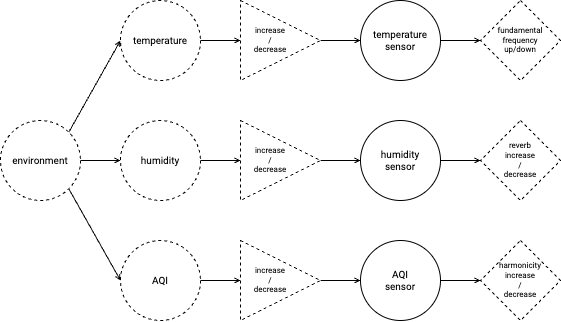
\includegraphics[width=0.7\linewidth]{chapters/3-mdc_model-reactivation_workflow-instruction_template/image/graph03-BVLconcept.png}
    \caption{Description of the installation through Baalman’s Visual Language - Conceptual level.}
    \label{fig:c3-BVLconceptual}
\end{figure} 
\begin{figure}[!h]
    \centering
    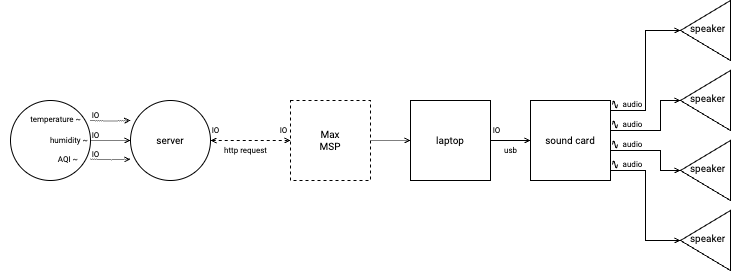
\includegraphics[width=0.7\linewidth]{chapters/3-mdc_model-reactivation_workflow-instruction_template/image/graph03-BVLphysical.png}
    \caption{Description of the installation through Baalman’s Visual Language - Physical implementation level.}
    \label{fig:c3-BVLphysical}
\end{figure} 
\begin{figure}[!h]
    \centering
    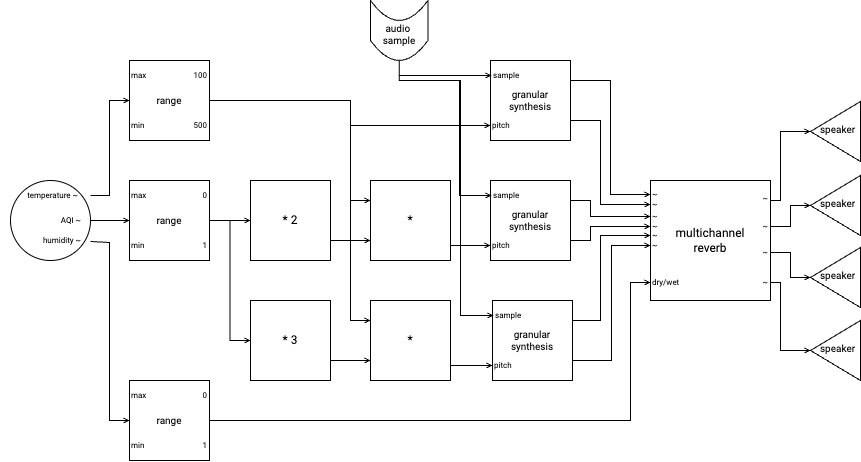
\includegraphics[width=0.7\linewidth]{chapters/3-mdc_model-reactivation_workflow-instruction_template/image/graph03-BVLprocess.png}
    \caption{Description of the installation through Baalman’s Visual Language - Process level (Highest level of representation).}
    \label{fig:c3-BVLprocess}
\end{figure} 
Figures~\ref{fig:c3-BVLconceptual}, ~\ref{fig:c3-BVLphysical} and ~\ref{fig:c3-BVLprocess} are some examples of how this visual language was applied in a creative case study aimed at studying the application of live media art installation documentation\footnote{This case study will not be explored in depth through a separate chapter unlike the other studies mentioned so far. We have chosen to omit it for the brevity and simplicity of the study, even though it was useful for exploring the application of BVL.}. In short, the study involves creating and documenting a sound installation in which data from a public air quality monitoring station controls the parameters of sound played in a room through four speakers.\\
Figure~\ref{fig:c3-BVLconceptual} shows the \textit{Conceptual level}, Figure~\ref{fig:c3-BVLphysical} shows the \textit{Physical implementation level}, and Figure~\ref{fig:c3-BVLprocess} shows the \textit{Process level} (shown at a high level, meaning you can zoom in and add more detail to the process).\\
This BVL is very useful, mainly because it remains flexible, allowing for creating new blocks and connections as needed. Its usage is also very versatile and fits well with the meta-model described earlier, as it can be applied to different levels of complexity. One can even use the visual language to hand-draw a mapping on paper, without needing any specific tools. Indeed, we will apply BVL in this thesis to represent the mappings of the case studies. In the next chapter, we will adapt the BVL to be used with Diagram.net, an online, free, and cross-platform system that can be used to draw diagrams.\\
However, while this language is adequate for describing process mappings, it does not address other crucial types of mappings, such as \textit{Temporal mapping} (e.g., what happens during a performance and when specific actions occur) and \textit{Spatial mapping} (e.g., the relationship between \textit{bit}s and physical space, such as a stage or a room). The stage plans used in live electronic music scores for \textit{Spatial mapping} remain highly effective, while defining \textit{Temporal mapping} is more complex. Generally, we must rely on something other than the musical notation system. As a result, this mapping type remains more open, varying from case to case\footnote{It is important to note that temporal mapping is especially useful in performance contexts. For example, in interactive installations, there is usually no need to guide the timing of interactions between gestures and the artwork made by the actors (such as the audience, the environment, or other factors). In interactive installations, a set of gestures and their relationships to the artwork are typically defined before implementation, but without specifying the order in which these gestures occur. The gestures appear randomly, depending on how actors interact with the piece.}. We can use graphical representations (either stylised or sequential, such as in the case study of Michele Sambin’s \textit{videoloop} in Appendix~\ref{ax:a-michele_sambin_videoloop}), written descriptions, custom notational systems (which would require a legend and preliminary definitions), multimedia files, or specific tools\footnote{Some tools are those developed for motion notation, especially in dance, by the \textit{Motion Bank} project at the University of Applied Sciences Frankfurt \url{https://motionbank.org/} (accessed 10/010/2024). Another interesting project is that one proposed by University of Udine’s Camera Ottica Laboratory for the classification of moving image \cite{costronuovo2024toward}.}.\\
Based on electronic music scores and BVL, we can define the \textit{Modular Instruction Framework} (MIF). The MIF is a template composed of multiple modules, each serving a specific informative function for compiling instructions to reactivate a creative work. Its modular design provides greater freedom when completing each module–none of the forms are mandatory–and, most importantly, allows them to be updated and changed over the course of the work’s various iterations.
\begin{itemize}
    \item \textit{Bit lists and specifications}: A textual document containing a list of all the bits (components) used in the artwork, with possible definitions and specifications. Multiple lists can be drawn up according to specific criteria (like electronic music scores, where you might have lists for acoustic instruments, electroacoustic instruments, and sound processing tools).
    \item \textit{Concepts and Notes}: A textual file that contains information about the artwork's identity, with various notes about the work itself or the instructions (e.g., who wrote the instructions and how they were written).
    \item \textit{Mappings}: Multiple documentation with all the mappings defined from different perspectives. This section can include the following sub-parts:
    \begin{itemize}
        \item \textit{Legend and Note}: Introduction and definition of the visual language used to describe the mappings.
        \item \textit{Parameters}: Any specific parameters related to the \textit{bit}s.
        \item \textit{Concept}: The conceptual level of the BVL, which can be expanded with additional text.
        \item \textit{Physical}: The physical implementation level of the BVL, which is also expandable by text.
        \item \textit{Process}: The process level of the BVL, again with extra explanation.
        \item \textit{Spatial}: The arrangement of \textit{bit}s and actors in space, which can be represented through a stage plan (or, more generally, a space plan).
        \item \textit{Temporal}: The definition of gesture-to-artwork relationships in the time domain. These mappings involve open graphical representations that should be explained in the Legend and Note section.
    \end{itemize}
    \item \textit{Graphical Information}: Multiple documents with text and images or diagrams that provide more detailed explanations of specific instructions (especially regarding the visual appearance of the artwork).
\end{itemize}

Examples of the MIF application can be seen in Appendices~\ref{ax:a-michele_sambin_videoloop}, ~\ref{ax:b-hybrid_reactivation_il_caos_delle_sfere}, \ref{ax:c-the_score_in_live_electronics_music}, and \ref{ax:d-sustainability_and_longevity_of_nimes}.  


\section{Summary}
The systems introduced in this chapter are closely based on the new conservation paradigms and serve as a synthesis of them. They allow for a practical visualisation of these paradigms and, therefore, the entire state of the art.
The MDC model, as a meta-model, does not define a specific conservation model but rather outlines the properties of creative works in relation to their conservation, focusing on the relationships between the various components and the quality of becoming. We define \textit{bit}s, \textit{data}, and \textit{experience} within their hierarchical structure. Still, we do not define their essence (except as an example)—whether digital or physical documentation, software or hardware components, etc. Thus, although we have seen that documentation plays a central role in conservation, the MDC model is not exclusively intended for it. This flexibility is why the MDC distinguishes it from the other models we have discussed so far and also why we intended it as a meta-model (even if it differs from the general understanding of meta-models used in computer science). As mentioned several times throughout this text, the artwork's materiality may be secondary to the documentation, but eliminating it is not always possible. Depending on the creative work or the choices made by an institution or one or more conservators, material elements can become part of the conservation process and thus be included within the MDC model. Therefore, the meta prefix should be seen as a way of surpassing a defined model but still providing a framework for creating and describing the conservation of live media art.\\
We can highlight the multilayered and dynamic qualities to compare the MDC model with the state-of-the-art and conservation paradigms. Starting with the multilayered aspect, we saw that it is defined from the first version of the model (based on the preservation framework for scientific data used in computer science) and the analogy of creative works as a multi-typological archive, alongside the use of ISAD(G). We have already seen something very similar in the documentation model developed by the DOCAM research alliance. The \textit{DOCAM Documentation Model} is based on and extends the \textit{Functional Requirements for Bibliographic Records} (1998) \cite{plassard1998functional} of the IFLA Study Group. The extension adds the component sublevel, which is ``\textit{at the very heart of the changes affecting most media artworks}''\footnote{For more details on the \textit{DOCAM Documentation Model}, please refer to Chapter~\ref{ch:1-state_of_the_art} or visit the DOCAM research aliance's website at the following link: \url{https://www.docam.ca/en/documentation-model.html} (last accessed 16/12/2024). Further information about the \textit{Functional Requirements for Bibliographic Records} (1998) can be found at the following link: \url{https://repository.ifla.org/items/54925d49-b08d-4aeb-807c-1b509ec40b55} (last accessed 16/12/2024).} The MDC model can, in turn, be seen as an extension of the \textit{DOCAM Documentation Model}. Figure~\ref{fig:c3-mdc-docam} shows a comparison between the \textit{DOCAM Documentation Model} and the MDC multilayering properties.
\begin{figure}[!h]
    \centering
    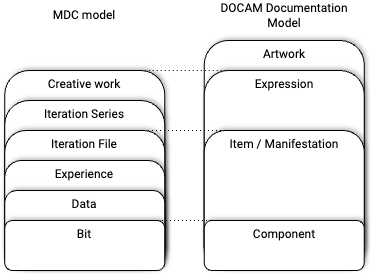
\includegraphics[width=0.5\linewidth]{chapters/3-mdc_model-reactivation_workflow-instruction_template/image/graph03-mdc-docam.png}
    \caption{Comparison between the \textit{DOCAM Documentation Model} and the MDC Model as extension in the multilayering property}
    \label{fig:c3-mdc-docam}
\end{figure}
Regarding the model’s dynamic quality, we see that the \textit{Iteration Series} (IS) tracks the artwork’s biography, and the property of \textit{multiple belongingness} allows for a fluid tracking of transformations and, therefore, identity. Although the dynamic character of the model follows examples from previous models, especially the \textit{Documentation Model for Time-based Media Art} by Joanna Phillips \cite{phillips2015reporting}, it goes beyond them, particularly in its relationship with identity. This model aims to surpass the \textit{allographic} and \textit{two-stage} concept, not considering the relationship from identity to manifestation (dynamic authenticity) as one-directional but bidirectional (as shown in Figure\~\ref{fig:c2-authenticity}), or rather, as expressed by the model itself, as a property. For this reason, we chose a matryoshka structure. In the MDC model, the manifestations within the IS are also within the \textit{Creative Work}. Therefore, the series of manifestations are properties of the \textit{Creative Work} and thus define its identity.\\
The property of \textit{dependency} in the MDC model is also significant, especially in relation to the \textit{ecological turn} discussed in the previous chapter. The dependency of levels and items on entities allows us to track the transformation of the artwork and view it in relation to the actors (\textit{actants}) responsible for that transformation. By visualising the dependencies of the artwork across various levels, we can reconstruct the dynamic ecology of its existence and, therefore, the interaction of the different ecosystems at play across the iterations.\\
If we compare the CATTA reactivation workflow with the MDC model, the former is essentially an extension of conservation, representing the loop between documentation and reactivation. Figure~\ref{fig:c3-mdc-catta} shows the relationship between the two systems.
\begin{figure}[!h]
    \centering
    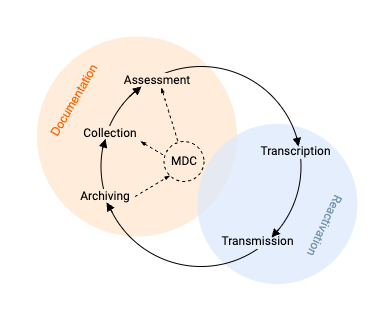
\includegraphics[width=0.8\linewidth]{chapters/3-mdc_model-reactivation_workflow-instruction_template/image/graph03-mdc-catta.png}
    \caption{The CATTA process extends the loop between documentation and reactivation discussed in the previous chapter. In this context, the MDC model serves as a tool used at both the beginning and end of each iteration, facilitating the archiving, collection, and assessment of documentation related to the artwork.}
    \label{fig:c3-mdc-catta}
\end{figure}
As summarised by the figure, the \textit{Collection}, \textit{Assessment} and \textit{Archiving} deal with the documentation and relate to the MDC model. At the same time, \textit{Transcription} and \textit{Transmission} are the two actions that occur during the reactivation. In this case, the MDC model is an instrument for archiving and then collecting and assessing the documentation for each reactivation.\\
Finally, the last element we introduced is the \textit{Modular Instruction Framework} (MIF), a set of optional modules used to create reactivation instructions for a creative work. The MIF is the result of combining the electronic music scores analyzed in Appendix~\ref{ax:c-the_score_in_live_electronics_music} with Baalman’s Visual Language (BVL).\\
Regarding the MIF, it’s important to note that compiling comprehensive instructions can be time-consuming, depending on how complex the work is and how much detail is needed. As mentioned earlier, the \textit{data} level is crucial for conservation. The more detailed this level becomes, the more the artwork’s identity is fixed—which, as discussed in the previous chapter, may not always be necessary for the work itself or for the artists and conservators involved.



    
    \chapter{\label{ch:4-madc_model_application}MDC Model Application and BVL adaptation}

In this chapter, we will explore the application of the \textit{Multilevel Dynamic Conservation} (MDC) Model as a Documentation Model for digital archives. Therefore, we will define a descriptive metadata structure for creative works and apply it through two very different development platforms – Neo4j and GitHub repositories – as well as a file management system, Finder. These systems represent distinct application scenarios, which is why they were selected. Neo4j is a graph database management system (GDBMS) that is particularly powerful in applications involving complex relationships between data\footnote{Some of the most famous application to use Neo4j are Linkedin, Netflix, PayPal, eBay, Uber, etc.}. GitHub is a collaborative version control platform for developers, allowing the creation, storage, management, and sharing of code and multimedia files. Finder is the Macintosh operating system's file manager and graphical user interface for organising folders and files and launching applications. The descriptive metadata schemes used in the three applications are adopted from existing descriptive and metadata systems, more or less specific to artworks and creative works. The organisation and structure of these metadata schemas will differ slightly across the three application systems, as each has its own development and application tools.\\
We wanted to apply the MDC model to these very different systems to highlight its abstraction and independence from any specific development platform while showcasing its adaptability. As emphasised in the previous chapter, this is the main strength of the model and the reason why we have called it a meta-model: it describes how a conservation model should be modelled and thus can be applied to different scenarios, with different levels of complexity and definition, without requiring specialised application skills. The application of the MDC model on these systems is illustrated by the case studies presented in Appendices~\ref{ax:a-michele_sambin_videoloop}, \ref{ax:b-hybrid_reactivation_il_caos_delle_sfere}, \ref{ax:c-the_score_in_live_electronics_music}, and \ref{ax:d-sustainability_and_longevity_of_nimes}. Appendices~\ref{ax:a-michele_sambin_videoloop} and \ref{ax:b-hybrid_reactivation_il_caos_delle_sfere} describe two complex artworks archived through Neo4j. Appendix~\ref{ax:d-sustainability_and_longevity_of_nimes} discusses two case studies related to research projects in the NIME field, archived and documented through a GitHub repository. Finally, Appendix~\ref{ax:c-the_score_in_live_electronics_music} focuses on the reactivation and study of scores from live electronic music works, which were stored using Finder for organising personal documentation and files (``actor archive''). We will refer to these case studies when presenting the various systems and their use according to the MDC model. Please refer to the respective chapters for more details about the case studies.\\
At the end of this chapter, we will also cover the adaptation of \textit{Baalman Visual Language} (BVL) used for the Modular Instruction Framework (MIF). In addition to the book Composing Interaction (Baalman, 2023), there is a repository where the BVL's author provides materials for using the language\footnote{\url{https://github.com/composing-interactions/ci-visual-language?tab=readme-ov-file} (last access 15/11/201)}. The repository includes SVG and PNG files with various blocks, arrows, and fonts. In the case studies discussed, we chose not to use the provided files as we found them somewhat tricky and especially limiting. Therefore, we decided to move away from the original graphical aspect of the language but extracted its key concepts (level division, differentiations and connections between blocks, etc.). The graphic reconstruction of the model was done using Diagrams.net, a cross-platform, online graph drawing software for creating diagrams such as flowcharts, wireframes, network diagrams, and more. In this case, we applied Baalman’s logic and concepts independently of the graphical language in a different environment.\\
The language was also applied to the case studies, and we will provide some examples from the studies in this context.\\
This chapter does not discuss the application of the CATTA reactivation workflow. Indeed, the reactivation process is explained for each case study, following the various steps during reactivation. Therefore, to see the application of the CATTA reactivation workflow, please refer to Appendices~\ref{ax:a-michele_sambin_videoloop}, \ref{ax:b-hybrid_reactivation_il_caos_delle_sfere}, ~\ref{ax:c-the_score_in_live_electronics_music}, and \ref{ax:d-sustainability_and_longevity_of_nimes}.

\section{Descriptive metadata schema and structure}
Before discussing the application of the MDC model through the different systems, it is essential to introduce the metadata schemas used to describe the various archived items and their relation and organisation. In this application, we did not introduce novel metadata schemas but instead adopted existing ones for the different types of descriptions needed for archiving. In this case, we used descriptive metadata schemas that were useful for describing the artworks and research projects covered in the case studies, which included different types of items. These include sensors, computers, smartphones, audio and video equipment, software, musical instruments, self-made boxes as well as artworks, the people and organisation involved, the iterations of the works, and more. Each of these elements requires specific and different fields of description.\\
Below, we list the main descriptive metadata schemas used in the archive and their application in the context of the MDC model.

\subsection{Artwork and iterations}
Although partially, the description of the creative work, which corresponds to the first macro level of the MDC model, can relate to the \textit{Identity Reports} developed and used by museums. Here, we consider six \textit{Identity Reports}: the one developed by the \textit{Media Conservation Initiative} (MCI) project at MoMA\footnote{MoMa’s Media Conservation Initiative (MCI)'s \textit{Identity Report} \url{https://static1.squarespace.com/static/5835fd7c15d5db57b19535bd/t/5c0042351ae6cf02642c2674/1543520821538/_Identity_Report_Template.pdf} (last accessed, 17/11/2024).}; the one developed by the \textit{Media Preservation Initiative} (MPI) project at the Whitney Museum of American Art\footnote{Whitney Museum of American Art’s Media Preservation Initiative (MPI)'s \textit{Identity report} \url{https://whitneymedia.org/assets/generic_file/1655/MPI_Identity_Report_Template.pdf} (last accessed, 17/11/2024).}; the one developed by the \textit{Time-based Media \& Digital Art Working Group} at the Smithsonian American Art Museum (SAAM)\footnote{ The SAAM’s Time-based Media \& Digital Art Working Group's \textit{Identity report} \url{https://whitneymedia.org/assets/generic_file/1655/MPI_Identity_Report_Template.pdf} (last accessed, 17/11/2024).}; the one developed by the Guggenheim\footnote{Guggenheim’s \textit{Identity Report} \url{https://www.guggenheim.org/wp-content/uploads/2019/12/guggenheim-identity-report-cant-help-myself-sun-yuan-peng-yu.pdf} (last accessed, 17/11/2024).}; the \textit{Cataloguing Form} developed by the DOCAM Research Alliance\footnote{The DOCAM cataloguing form \url{https://www.docam.ca/en/tools/cataloguing-form.html} (last accessed, 17/11/2024).}; and the \textit{Installation Specification} developed by the \textit{Matters in Media Art} project\footnote{The Matters in Media Art's Installation Specificiation can be found at the following link: \url{https://mattersinmediaart.org/acquiring-time-based-media-art.html} (last accessed, 17/11/2024).}
.\\
All the \textit{Identity Reports} share many common sections, as we have already seen in Cahpter~\ref{ch:1-state_of_the_art} when referring to the Guggenheim \textit{Identity Report}. Here, we can summarise these sections as follows: 1) \textit{Identification} (Artwork identification), 2) \textit{Description} (identity of the artwork), 3) \textit{History of Exhibitions and Iterations}, 4) \textit{Anatomy of the Artwork}, 5) \textit{Risk and Resources}, 6) \textit{Installation Parameters}, and 7) \textit{Technical Requirements and Parameters}. It is clear that when using the MDC model, the various fields of the \textit{Identity Report} are distributed across the different sub-levels of the archive. The \textit{History of Exhibitions and Iterations} and all description fields are used at the individual \textit{Iteration File} (IF) level. \textit{Anatomy of the Artwork}, \textit{Installation Parameters}, and \textit{Technical Requirements and Parameters} are described at the \textit{bit} and \textit{data} levels. Only \textit{Identification}, \textit{Description}, and \textit{Risk and Resources} are used at the artwork level. Therefore, the artwork can be defined using with the fields in Table~\ref{tab:c4-artwork}.

\begin{longtable}{|p{0.35\textwidth}|p{0.15\textwidth}|p{0.4\textwidth}|}
    \caption{Artwork Metadata Schema} \label{tab:c4-artwork} \\
    \hline
    \textbf{Field} & \textbf{Value} & \textbf{Description} \\
    \hline
    \endfirsthead

    \scriptsize id                      & \scriptsize String                                            &  \scriptsize Item Identifier. \\
    \hline
    \scriptsize id:title                   & \scriptsize String                                            &  \scriptsize Title of the creative work.\\
    \hline
    \scriptsize id:dateCreated             & \scriptsize Date                                              &  \scriptsize The date of the creative work creation is in the format ISO8601 (e.g., yyyy-mm-dd).\\
    \hline
    \scriptsize id:artist                  & \scriptsize \textcolor{uniudColor3}{Person}[]                 &  \scriptsize The person(s) who created the creative work. \\
    \hline
    \scriptsize id:picture                 & \scriptsize \textcolor{uniudColor3}{Image}                    &  \scriptsize Link to a single image (\textit{experience} item) that represents the creative work. \\
    \hline
    \scriptsize id:description             & \scriptsize String                                            &  \scriptsize Description of the creative work. \\
    \hline
    \scriptsize id:conservationStatement   & \scriptsize String                                            &  \scriptsize A conservation statement with the essential aspects to consider in order to conserve the artwork.\\
    \hline
    \scriptsize id:iterationSeries         & \scriptsize \textcolor{uniudColor3}{Iteration}[]              &  \scriptsize A series of iterations (manifestations) of the creative work. \\
    \hline
    \scriptsize id:bibliographySeries      & \scriptsize \textcolor{uniudColor3}{Book}[] \textcolor{uniudColor3}{Paper}[] ...   &  \scriptsize A series of reference texts. \\
    \hline

\end{longtable}
Here, we decided to identify the artwork with the most general aspects, reducing the number of description fields. For example, the description of the artwork is usually divided into several sections, which cover the curatorial and artistic aspects, technical details, statements from the artists and collaborators, and so on. Here, we simplify this into a single \textit{description} field. The same applies to the \textit{conservationStatement} field. Additionally, we do not use the common field for \textit{medium} or \textit{medium lines}, which are typically used in \textit{identification}. The medium can be derived from the \textit{bit}s and \textit{data} for each \textit{Iteration File}.\\
The process for the \textit{Iteration Report} is very similar. Here, we focused on the \textit{Iteration Reports} from the Guggenheim\footnote{ Guggenheim’s \textit{Iteration Report} \url{https://www.guggenheim.org/wp-content/uploads/2015/11/guggenheim-conservation-iteration-report-2012.pdf} (last accessed, 18/11/2024).} and the \textit{Time-based Media \& Digital Art Working Group} at the Smithsonian American Art Museum (SAAM) \footnote{SAAM’s \textit{Iteration Report} \url{https://www.si.edu/tbma/resource/iteration-report} (last accessed, 18/11/2024).}– which are very similar – the \textit{Exhibition Report} from the \textit{Media Preservation Initiative} (MPI) project at the Whitney Museum of American Art\footnote{Whitney Msueum of American Art’s \textit{Exhibition Report} \url{https://whitneymedia.org/assets/generic_file/1657/MPI_Exhibition_Report_Template.pdf} (last accessed, 18/11/2024).}, and the \textit{Documentation for Technological Changes} from the DOCAM research alliance\footnote{DOCAM’s \textit{Documentation for technological changes} \url{https://www.docam.ca/en/tools/documentation-for-technological-changes.html} (last accessed, 18/11/2024).}. Therefore, each iteration is described with the fields in Table~\ref{tab:c4-iteration}.

\begin{longtable}{|p{0.35\textwidth}|p{0.15\textwidth}|p{0.4\textwidth}|}
    \caption{Iteration Metadata Schema} \label{tab:c4-iteration} \\
    \hline
    \textbf{Field} & \textbf{Value} & \textbf{Description} \\
    \hline
    \endfirsthead
    \scriptsize id                      & \scriptsize String                                            &  \scriptsize Item Identifier. \\
    \hline
    \scriptsize it:title                   & \scriptsize String, \textcolor{uniudColor3}{Event}            &  \scriptsize Event or Iteration/Exhibition title.\\
    \hline
    \scriptsize it:date                    & \scriptsize Date                                              &  \scriptsize The exhibition date in the format ISO8601 (e.g., yyyy-mm-dd). For describing the exhibition period: [startDate, endDate].\\
    \hline
    \scriptsize it:venue                   & \scriptsize \textcolor{uniudColor3}{Place}                    &  \scriptsize The Place in which the iteration took place. \\
    \hline
    \scriptsize it:curator, performer, mediaTechnichian, ...                 & \scriptsize \textcolor{uniudColor3}{Person}[]                    &  \scriptsize All the people involved in the iteration with their role\footnote{Based on the \textit{Iteration reports} studied we can have: \textit{Curator}(s), \textit{Exhibition Designer}(s), \textit{Media Technician}(s), \textit{Conservator}(s), \textit{Registrar}(s), \textit{Artist}(s), \textit{Artist Assistant}(s), \textit{Fabricator}(s), \textit{Art Handler}(s), \textit{Consultant}(s), \textit{External Company}, \textit{and Other}(s). The \textit{Iteration Reports} usually consider only exhibition such as installation and they do not include performers, that we would like to add in the description of the iteration since would be helpful to describe our case studies.}..\\
    \hline
    \scriptsize it:description             & \scriptsize String                                            &  \scriptsize Description of the iteration. \\
    \hline
    \scriptsize it:picture                 & \scriptsize \textcolor{uniudColor3}{Image}                    &  \scriptsize Link to a single \textit{experience} item that represents the iteration of the artwork.\\
    \hline
    \scriptsize it:note                    & \scriptsize String                                            &  \scriptsize Note about the iteration that can comprehend problems related to the installation and rehearsal, technological changes, and other essential details. \\
    \hline
    \scriptsize it:bit                     & \scriptsize \textcolor{uniudColor3}{AudioEquip}[], \textcolor{uniudColor3}{VideoEquip}[], ...   &  \scriptsize List of \textit{bit} items related to the iteration.\\
    \hline
   \scriptsize  it:data                    & \scriptsize \textcolor{uniudColor3}{Image}[], \textcolor{uniudColor3}{Doc}[], ...   &  \scriptsize List of \textit{data} items related to the iteration.\\
    \hline
    \scriptsize it:experience              & \scriptsize \textcolor{uniudColor3}{Image}[], \textcolor{uniudColor3}{Video}[], \textcolor{uniudColor3}{Paper}[], ...   &  \scriptsize List of \textit{experience} items related to the iteration.\\
    \hline
\end{longtable}

In this case, the description fields have also been significantly reduced compared to the \textit{Iteration Reports} we studied. Once again, much of the information from these reports is spread across the various upper and lower levels of the MDC model and can be easily derived by looking at the archive as a whole (as we will see in the following subsections).\\
Schema value types such as \textit{Person}, \textit{Image}, \textit{Video}, \textit{Iteration}, \textit{Book}, \textit{Paper} and so on (highlighted in blue in the tables) refer to other metadata schemas. For example, \textit{iterationSeries} in the \textit{Creative Work} metadata schema refers to multiple Iteration metadata schemas (multiple as indicated by the two square brackets).

\subsection{Person, organisation, place, and event}
We use the metadata schemas defined by \textit{Schema.org} as a model to describe entities related to the artworks and their iterations—such as person, organisation, event, and place. \textit{Schema.org} is a community-driven initiative focused on creating, maintaining, and promoting schemas for structured data across the Internet, including web pages, email messages, and more.\\
According to \textit{Schema.org}, we define in Table~\ref{tab:c4-person}, with some necessary adjustments for the description area, the \textit{Person} metadata schema.

\begin{longtable}{|p{0.35\textwidth}|p{0.15\textwidth}|p{0.4\textwidth}|}
    \caption{Person Metadata Schema} \label{tab:c4-person} \\
    \hline
    \textbf{Field} & \textbf{Value} & \textbf{Description} \\
    \hline

    \scriptsize id                      & \scriptsize String                                            &  \scriptsize Item Identifier. \\
    \hline
    \scriptsize pe:givenName               & \scriptsize String                                             &  \scriptsize The first name of a Person.\\
    \hline
    \scriptsize pe:familyName              & \scriptsize String                                             &  \scriptsize The last name of a Person.\\
    \hline
    \scriptsize pe:birthDate               & \scriptsize Date                                             &  \scriptsize Date of birth in the ISO8601 format.\\
    \hline
    \scriptsize pe:birthPlace              & \scriptsize \textcolor{uniudColor3}{Place}                    &  \scriptsize The place where the person was born.\\
    \hline
    \scriptsize pe:deathDate               & \scriptsize Date                                             &  \scriptsize Date of death in the ISO8601 format.\\
    \hline
    \scriptsize pe:deathPlace              & \scriptsize \textcolor{uniudColor3}{Place}                    &  \scriptsize The place where the person died.\\
    \hline
    \scriptsize pe:nationality             & \scriptsize String                                       &  \scriptsize Nationality of the person.\\
    \hline
    \scriptsize pe:biography               & \scriptsize String                                       &  \scriptsize A biography of the person.\\
    \hline
    \scriptsize pe:website                 & \scriptsize URL                                       &  \scriptsize Website of the person.\\
    \hline

\end{longtable}

Table~\ref{tab:c4-organisation} show the \textit{Organisation} metadata schema according to \textit{Scema.org}. In this context, the organization should be viewed as a group of people structured in either a private or institutional manner.

\begin{longtable}{|p{0.35\textwidth}|p{0.15\textwidth}|p{0.4\textwidth}|}
    \caption{Organisation Metadata Schema} \label{tab:c4-organisation} \\
    \hline
    \textbf{Field} & \textbf{Value} & \textbf{Description} \\
    \hline

    \scriptsize id                      & \scriptsize String                                            &  \scriptsize Item Identifier. \\
    \hline
    \scriptsize or:legalName             & \scriptsize String                                            &  \scriptsize The official name of the organisation. \\
    \hline
    \scriptsize or:address               & \scriptsize \textcolor{uniudColor3}{Place}[], Address         &  \scriptsize The organisation's physical address according to the Universal Postal Union (UDU) recommendation. \\
    \hline
    \scriptsize or:member                & \scriptsize \textcolor{uniudColor3}{Person}[], \textcolor{uniudColor3}{Organisation}[] &  \scriptsize Person(s) or Organisation(s) members of the organisation. \\
    \hline
    \scriptsize or:description           & \scriptsize Text                                             &  \scriptsize Description of the organisation. \\
    \hline
    \scriptsize or:website                 & \scriptsize URL                                              & \scriptsize  Website of the organisation. \\
    \hline

\end{longtable}

Table~\ref{tab:c4-place} show the \textit{Place} metadata schema according to \textit{Scema.org}. 

\begin{longtable}{|p{0.35\textwidth}|p{0.15\textwidth}|p{0.4\textwidth}|}
    \caption{Place Metadata Schema} \label{tab:c4-place} \\
    \hline
    \textbf{Field} & \textbf{Value} & \textbf{Description} \\
    \hline

    \scriptsize id                      & \scriptsize String                                            &  \scriptsize Item Identifier. \\
    \hline
    \scriptsize pl:legalName             & \scriptsize String                                            &  \scriptsize The official name of the place. \\
    \hline
    \scriptsize pl:address               & \scriptsize Address                                          &  \scriptsize The place's physical address according to the Universal Postal Union (UDU) recommendation. \\
    \hline
    \scriptsize pl:description           & \scriptsize Text                                             &  \scriptsize Description of the place. \\
    \hline
    \scriptsize pl:website                 & \scriptsize URL                                              &  \scriptsize Website of the place. \\
    \hline

\end{longtable}

The last metadata schema referred to \textit{Schema.org} is the \textit{Event} metadata schema in Table~\ref{tab:c4-event}.

\begin{longtable}{|p{0.35\textwidth}|p{0.15\textwidth}|p{0.4\textwidth}|}
    \caption{Event Metadata Schema} \label{tab:c4-event} \\
    \hline
    \textbf{Field} & \textbf{Value} & \textbf{Description} \\
    \hline

    \scriptsize id                      & \scriptsize String                                            &  \scriptsize Item Identifier. \\
    \hline
    \scriptsize ev:name                  & \scriptsize String                                            &  \scriptsize Name of the event. \\
    \hline
    \scriptsize ev:startDate             & \scriptsize Date                                              &  \scriptsize Beginning of the event in the ISO8601 format. \\
    \hline
    \scriptsize ev:endDate               & \scriptsize Date                                              &  \scriptsize End of the event in the ISO8601 format. \\
    \hline
    \scriptsize ev:location              & \scriptsize \textcolor{uniudColor3}{Place}                    &  \scriptsize The place in which the event took place. \\
    \hline
    \scriptsize ev:organiser             & \scriptsize \textcolor{uniudColor3}{Person[]}, \textcolor{uniudColor3}{Organisation[]}   &  \scriptsize Organiser(s) of the event. \\
    \hline
    \scriptsize ev:description           & \scriptsize String                                            &  \scriptsize Description of the event. \\
    \hline
    \scriptsize ev:website                 & \scriptsize URL                                              & \scriptsize  Website of the event. \\
    \hline

\end{longtable}

For each type of metadata schema, we selected the essential fields (which can be extended by referring to the original metadata schema\footnote{\textit{Person} Metadata schema \url{https://schema.org/Person} (last accessed 17/11/2024); \textit{Organisation} Metadata schema \url{https://schema.org/Organization} (last accessed 17/11/2024); \textit{Place} metadata schema \url{https://schema.org/Place} (last accessed 17/11/2024); \textit{Event} metadata schema \url{https://schema.org/Event} (last accessed 17/11/2024).}). We added specific fields, such as \textit{biography} in the \textit{Person} schema (where the original \textit{description} field could be used) and \textit{website} for all.

\subsection{Audio and video equipments}
There are no specific standards for describing audio physical devices, such as audio mixers, sound cards, microphones, etc. However, we can combine the general description from \textit{Dublin Core} with the technical specifications from the Audio Engineering Society's AES57 standard \cite{AES57}.\\
The description of an audio mixer could follow these fields in Table~\ref{tab:c4-mixer}.

\begin{longtable}{|p{0.35\textwidth}|p{0.15\textwidth}|p{0.4\textwidth}|}
    \caption{Mixer Metadata Schema} \label{tab:c4-mixer} \\
    \hline
    \textbf{Field} & \textbf{Value} & \textbf{Description} \\
    \hline

    \scriptsize id                      & \scriptsize String           & \scriptsize Item Identifier. \\
    \hline
    \scriptsize db:title                & \scriptsize String           & \scriptsize The name and model of the mixer. \\
    \hline
    \scriptsize db:description          & \scriptsize String           & \scriptsize A brief summary of the mixer's features and specifications. \\
    \hline
    \scriptsize db:subject              & \scriptsize String           & \scriptsize A brief description of the mixer's primary purpose or application. \\
    \hline
    \scriptsize db:dateCreated          & \scriptsize Date             & \scriptsize The creation date of the equipment in ISO8601 format. \\
    \hline
    \scriptsize db:creator              & \scriptsize \textcolor{uniudColor3}{Person}[], \textcolor{uniudColor3}{Organisation}[], String & \scriptsize Person(s) or organization(s) that created the mixer. \\
    \hline
    \scriptsize db:publisher            & \scriptsize \textcolor{uniudColor3}{Person}[], \textcolor{uniudColor3}{Organisation}[], String & \scriptsize Publisher or manufacturer of the mixer. \\
    \hline
    \scriptsize db:format               & \scriptsize String           & \scriptsize Specifies the format or category of the mixer (e.g., Analog Mixing Console). \\
    \hline
    \scriptsize db:relation             & \scriptsize String           & \scriptsize Identifies the series or family to which the mixer belongs. \\
    \hline
    \scriptsize eas57:analogInterfaces  & \scriptsize String           & \scriptsize Specifies the analog input/output interfaces available on the device. \\
    \hline
    \scriptsize eas57:audioDataEncoding & \scriptsize String           & \scriptsize Indicates the type of audio data encoding, such as analog or digital. \\
    \hline
    \scriptsize eas57:dynamicRange      & \scriptsize String           & \scriptsize The dynamic range of the equipment, typically measured in dB. \\
    \hline
    \scriptsize eas57:numberOfChannels  & \scriptsize Integer          & \scriptsize The number of channels the equipment can handle. \\
    \hline
    \scriptsize eas57:powerRequirements & \scriptsize String           & \scriptsize Details about the equipment's power source or requirements. \\
    \hline
    \scriptsize eas57:signalToNoiseRatio& \scriptsize String           & \scriptsize The signal-to-noise ratio, typically measured in dB, indicating audio clarity. \\
    \hline
    \scriptsize eas57:dimensions        & \scriptsize String           & \scriptsize The physical dimensions of the equipment in width x height x depth format. \\
    \hline
    \scriptsize eas57:weight            & \scriptsize String           & \scriptsize The weight of the equipment, typically measured in kilograms. \\
    \hline

\end{longtable}

Similarly, no specific standards exist for describing video physical devices—such as LCD screens, cameras, etc. Again, we use \textit{Dublin Core} for general descriptive metadata, combined with the technical standards from the Society of Motion Picture and Television Engineers \cite{SMPTE}, which capture technical specifications.\\
The description of a generic LCD monitor could follow the fields listed in Table~\ref{tab:c4-video}.

\begin{longtable}{|p{0.35\textwidth}|p{0.15\textwidth}|p{0.4\textwidth}|}
    \caption{Monitor Metadata Schema} \label{tab:c4-monitor} \\
    \hline
    \textbf{Field} & \textbf{Value} & \textbf{Description} \\
    \hline

    \scriptsize id                      & \scriptsize String           & \scriptsize Item Identifier. \\
    \hline
    dc:title                & \scriptsize String           & \scriptsize The name and model of the monitor. \\
    \hline
    \scriptsize dc:description          & \scriptsize String           & \scriptsize A brief summary of the monitor's features and specifications. \\
    \hline
    \scriptsize dc:subject              & \scriptsize String           & \scriptsize A brief description of the monitor's primary purpose or classification. \\
    \hline
    \scriptsize dc:dateCreated          & \scriptsize Date             & \scriptsize The release or creation date of the monitor in ISO8601 format. \\
    \hline
    \scriptsize dc:creator              & \scriptsize \scriptsize \textcolor{uniudColor3}{Person}[], \textcolor{uniudColor3}{Organisation}[], String           & \scriptsize Person(s) or Organization(s) that created the monitor. \\
    \hline
    \scriptsize dc:publisher            & \scriptsize \scriptsize \textcolor{uniudColor3}{Person}[], \textcolor{uniudColor3}{Organisation}[], String           & \scriptsize Person(s) or Organization(s) responsible for producing the monitor. \\
    \hline
    \scriptsize dc:format               & \scriptsize String           & \scriptsize The format and specifications of the monitor, such as resolution and technology. \\
    \hline
    \scriptsize dc:relation             & \scriptsize String           & \scriptsize The series or family to which the monitor belongs. \\
    \hline
    \scriptsize smpte:aspectRatio      & \scriptsize String           & \scriptsize The ratio of the width to the height of the display. \\
    \hline
    \scriptsize smpte:brightness        & \scriptsize String           & \scriptsize The brightness of the display, typically measured in cd/m². \\
    \hline
    \scriptsize smpte:colorSpace       & \scriptsize String           & \scriptsize The color space supported by the display, such as sRGB. \\
    \hline
    \scriptsize smpte:contrastRatio    & \scriptsize String           & \scriptsize The contrast ratio, which measures the difference between the darkest and brightest output. \\
    \hline
    \scriptsize smpte:contributor       & \scriptsize String           & \scriptsize The individual or team that contributed to the product development. \\
    \hline
    \scriptsize smpte:coverage          & \scriptsize String           & \scriptsize The geographical coverage or availability of the product. \\
    \hline
    \scriptsize smpte:frameRate        & \scriptsize String           & \scriptsize The maximum refresh rate of the display, measured in Hz. \\
    \hline
    \scriptsize smpte:interface         & \scriptsize String           & \scriptsize The input/output interfaces supported by the monitor, such as HDMI or VGA. \\
    \hline
    \scriptsize smpte:powerConsumption & \scriptsize String           & \scriptsize The amount of power the monitor consumes, typically measured in watts. \\
    \hline
    \scriptsize smpte:resolution        & \scriptsize String           & \scriptsize The resolution of the display in pixels, such as 1920x1080. \\
    \hline
    \scriptsize smpte:syncSupport      & \scriptsize String           & \scriptsize The synchronization technology supported by the monitor, such as FreeSync. \\
    \hline

\end{longtable}


\subsection{Computer hardware and software}
To describe desktop computers, laptops, single-board computers, microcontrollers, and commercial application software, we can use the \textit{Common Information Model} (CIM) standard developed by the Distributed Management Task Force (DMTF) \cite{CIM}. The CIM standard provides a framework for describing the management of information technology (IT) infrastructure, including hardware, software, and network resources. This system is powerful because it allows for a clear separation of various computer components, such as processors, RAM, storage, etc., and also helps establish relationships with software components.\\
An example of a computer system described using the CIM metadata schema is in table~\ref{tab:c4-computer}

\begin{longtable}{|p{0.45\textwidth}|p{0.15\textwidth}|p{0.3\textwidth}|}
    \caption{Computer System Metadata Schema} \label{tab:c4-computer} \\
    \hline
    \textbf{Field} & \textbf{Value} & \textbf{Description} \\
    \hline

    \scriptsize id                                    & \scriptsize String                         & \scriptsize Item Identifier. \\
    \hline
    \scriptsize cim:ComputerSystem.elementName        & \scriptsize String                         & \scriptsize The name of the laptop computer system. \\
    \hline
    \scriptsize cim:ComputerSystem.Name               & \scriptsize String                         & \scriptsize The model name of the laptop. \\
    \hline
    \scriptsize cim:ComputerSystem.Manufacturer       & \scriptsize String, \textcolor{uniudColor3}{Organisation}[], \textcolor{uniudColor3}{Person}[]     & \scriptsize The manufacturer of the laptop. \\
    \hline
    \scriptsize cim:ComputerSystem.Model              & \scriptsize String                         & \scriptsize The model number or specific name of the laptop. \\
    \hline
    \scriptsize cim:ComputerSystem.OperatingSystem    & \scriptsize \textcolor{uniudColor3}{cim:OperatingSystem}[]          & \scriptsize The operating system installed on the laptop. \\
    \hline
    \scriptsize cim:ComputerSystem.Processor          & \scriptsize \textcolor{uniudColor3}{cim:Processor}[]                & \scriptsize The processor(s) installed on the laptop. \\
    \hline
    \scriptsize cim:ComputerSystem.Memory             & \scriptsize \textcolor{uniudColor3}{cim:Memory}[]                   & \scriptsize The memory(s) installed on the laptop. \\
    \hline
    \scriptsize cim:ComputerSystem:StorageVolume      & \scriptsize \textcolor{uniudColor3}{cim:StorageVolume}[]            & \scriptsize The storage volume(s) installed on the laptop. \\
    \hline
    \scriptsize cim:ComputerSystem:Display            & \scriptsize \textcolor{uniudColor3}{smpte:Display}                  & \scriptsize The display of the laptop. \\
    \hline
    \scriptsize …                                     & \scriptsize …                              & \scriptsize … \\
    \hline

\end{longtable}

In this case, the values \textit{cim:OperatingSystem}, \textit{cim:Processor}, \textit{cim:Memory}, \textit{cim:StorageVolume} and many others refer to relations to other CIM metadata schemas. The \textit{smpte:Display} can be related to the \textit{Monitor} Metadata Schema, and the same thing could be done for a sound card and other Audio or Video Equipments.
An example of a metadata schema for the \textit{operating system} is in table~\ref{tab:c4-os}

\begin{longtable}{|p{0.45\textwidth}|p{0.15\textwidth}|p{0.3\textwidth}|}
    \caption{Operating System Metadata Schema} \label{tab:c4-os} \\
    \hline
    \textbf{Field} & \textbf{Value} & \textbf{Description} \\
    \hline

    \scriptsize id                                    & \scriptsize String                         & \scriptsize Item Identifier. \\
    \hline
    \scriptsize cim:OperatingSystem.elementName       & \scriptsize String                         & \scriptsize The name of the Operating system. \\
    \hline
    \scriptsize cim:ComputerSystem.Name               & \scriptsize String                         & \scriptsize The model name of the operating system. \\
    \hline
    \scriptsize cim:OperatingSystem.Manufacturer      & \scriptsize String, \textcolor{uniudColor3}{Organisation}, \textcolor{uniudColor3}{Person}     & \scriptsize The manufacturer of the Operating System. \\
    \hline
    \scriptsize cim:OperatingSystem.OSArchitecture    & \scriptsize String                         & \scriptsize The operating system's architecture (e.g., x64, x86, ARM). \\
    \hline
    \scriptsize cim:OperatingSystem.OSType            & \scriptsize String                         & \scriptsize The operating system type (e.g., Desktop, Server, Embedded). \\
    \hline
    \scriptsize cim:OperatingSystem.Platform          & \scriptsize String                         & \scriptsize The platform that the operating system is designed to run on (e.g., Windows). \\
    \hline
    \scriptsize …                                     & \scriptsize …                              & \scriptsize … \\
    \hline

\end{longtable}

For software applications, we can also use the CIM standard, as shown in table~\ref{tab:c4-software}:

\begin{longtable}{|p{0.45\textwidth}|p{0.15\textwidth}|p{0.3\textwidth}|}
    \caption{Software Application Metadata Schema} \label{tab:c4-software} \\
    \hline
    \textbf{Field} & \textbf{Value} & \textbf{Description} \\
    \hline

    \scriptsize id                                    & \scriptsize String                         & \scriptsize Item Identifier. \\
    \hline
    \scriptsize cim:SoftwareElement.ElementName       & \scriptsize String                         & \scriptsize The name of the software application. \\
    \hline
    \scriptsize cim:SoftwareElement.Name              & \scriptsize String                         & \scriptsize The full name and version of the software application. \\
    \hline
    \scriptsize cim:SoftwareElement.Manufacturer      & \scriptsize String, \textcolor{uniudColor3}{Organisation}, \textcolor{uniudColor3}{Person}     & \scriptsize The manufacturer of the software application. \\
    \hline
    \scriptsize cim:SoftwareElement.Version           & \scriptsize String                         & \scriptsize The version number of the software. \\
    \hline
    \scriptsize cim:SoftwareElement.OperatingSystem   & \scriptsize \textcolor{uniudColor3}{cim:OperatingSystem}[]          & \scriptsize The operating systems supported by the software. \\
    \hline
    \scriptsize cim:SoftwareElement.Description       & \scriptsize String                         & \scriptsize A brief description of the software’s purpose and functionality. \\
    \hline
    …                                     & \scriptsize …                              & … \\
    \hline

\end{longtable}

For non-commercial, original software, we have chosen to use \textit{CodeMeta}, a metadata schema developed for scientific research. It is designed to facilitate the sharing and reusing code and software\footnote{Codemeta project website \url{https://codemeta.github.io/} (last accessed 19/11/2024).}. An example is given in table~\ref{tab:c4-original-software} \footnote{To generate a metadata schema with the \textit{CodeMeta Generator v3.0} at the link \url{https://codemeta.github.io/codemeta-generator/} (last accessed 19/11/2024).}
.

\begin{longtable}{|p{0.45\textwidth}|p{0.15\textwidth}|p{0.3\textwidth}|}
    \caption{Original Software Metadata Schema} \label{tab:c4-original-software} \\
    \hline
    \textbf{Field} & \textbf{Value} & \textbf{Description} \\
    \hline

    \scriptsize id                                    & \scriptsize String                         & \scriptsize Item Identifier. \\
    \hline
    \scriptsize cm:Name                               & \scriptsize String                         & \scriptsize The name of the original software. \\
    \hline
    \scriptsize cm:Description                        & \scriptsize String                         & \scriptsize Description of the software. \\
    \hline
    \scriptsize cm:CreationDate                       & \scriptsize Date                           & \scriptsize Date of the software creation according to the ISO8601 format. \\
    \hline
   \scriptsize  cm:FirstReleaseDate                   & \scriptsize Date                           & \scriptsize Date of the first software release according to the ISO8601 format. \\
    \hline
    \scriptsize cm:License                            & \scriptsize URL[]                          & \scriptsize Attributed licence(s). \\
    \hline
    \scriptsize cm:UniqueIdentifier                   & \scriptsize String                         & \scriptsize An identifier for the software. \\
    \hline
    \scriptsize cm:Author                             & \scriptsize String, \textcolor{uniudColor3}{Person}[], \textcolor{uniudColor3}{Organisation}[]        & \scriptsize Person(s) or Organisation(s) that created the software. \\
    \hline
    \scriptsize cm:Keywords                           & \scriptsize String                         & \scriptsize Relevant keywords that describe the software. \\
    \hline
    \scriptsize cm:ProgrammingLanguage                & \scriptsize String, \textcolor{uniudColor3}{cim:SoftwareApplication} & \scriptsize The programming language with which the software has been developed (e.g. Java, Python, etc.). \\
    \hline
    \scriptsize cm:RuntimePlatform                    & \scriptsize String, \textcolor{uniudColor3}{cim:SoftwareApplication} & \scriptsize Runtime application for running the software (.NET, JVM, etc.). \\
    \hline
    \scriptsize cm:OperatingSystem                    & \scriptsize \textcolor{uniudColor3}{cim:OperatingSystem}            & \scriptsize Operating system for running the software. \\
    \hline
    \scriptsize cm:OtherSoftwareRequirement           & \scriptsize String, \textcolor{uniudColor3}{cim:SoftwareApplication}, URL & \scriptsize Other requirements include libraries, multimedia files, etc. \\
    \hline
    \scriptsize cm:VersionNumber                      & \scriptsize String                         & \scriptsize The current version of the software. \\
    \hline
    \scriptsize …                                     & \scriptsize …                              & \scriptsize … \\
    \hline

\end{longtable}

\subsection{Sensors}
\textit{Sensor Model Language} (SensorML) is a specific description system for various types of sensors \cite{SensorML}. It provides a structured and semantically linked way to define processes and components involved in measuring and transforming observations. SensorML also provides metadata schemas for sensors, actuators, and computational processes applied before and after measurements. Using this system, we can describe not only sensors but also potentiometers and other components typically used in creating original devices for artworks.\\
A metadata schema for a temperature sensor could follow the fields listed in table~\ref{tab:c4-sensor}:


\begin{longtable}{|p{0.35\textwidth}|p{0.15\textwidth}|p{0.4\textwidth}|}
    \caption{Sensor (Temperature Sensor) Metadata Schema} \label{tab:c4-temperature-sensor} \\
    \hline
    \textbf{Field} & \textbf{Value} & \textbf{Description} \\
    \hline

    \scriptsize …id                                    & \scriptsize String                         & \scriptsize …Item Identifier. \\
    \hline
    \scriptsize …sml:Sensor.Name                       & \scriptsize String                         & \scriptsize …The name or model of the temperature sensor. \\
    \hline
    \scriptsize …sml:Sensor.Description                & \scriptsize String                         & \scriptsize …A short description of the sensor’s functionality. \\
    \hline
    \scriptsize …sml:Sensor.Manufacturer               & \scriptsize String, \textcolor{uniudColor3}{Organisation}, \textcolor{uniudColor3}{Person}     & \scriptsize …The manufacturer of the temperature sensor. \\
    \hline
    \scriptsize …sml:Sensor.Model                      & \scriptsize String                         & \scriptsize …The specific model of the temperature sensor. \\
    \hline
    \scriptsize …sml:Sensor.Type                       & \scriptsize String                         & \scriptsize …The type of measurement the sensor is designed for (in this case, temperature). \\
    \hline
    \scriptsize …sml:Sensor.MeasurementUnit            & \scriptsize String                         & \scriptsize …The unit of measurement used by the sensor (e.g., Celsius, Fahrenheit). \\
    \hline
    \scriptsize …sml:Sensor.OperatingRange             & \scriptsize String                         & \scriptsize …The sensor's operational range indicates the minimum and maximum temperature it can measure. \\
    \hline
    \scriptsize …sml:Sensor.Sensitivity                & \scriptsize String                         & \scriptsize …The temperature sensor's sensitivity represents the smallest detectable change in temperature. \\
    \hline
    \scriptsize …sml:Sensor.Accuracy                   & \scriptsize String                         & \scriptsize …The accuracy of the temperature measurements provided by the sensor. \\
    \hline
    \scriptsize ……                                     & \scriptsize …                              & \scriptsize …… \\
    \hline

\end{longtable}

\subsection{Multimedia files}
Many metadata schema standards exist for multimedia files, such as audio and video. In this case, we have adopted the multimedia content description standard from the Moving Picture Experts Group, MPEG-7 \cite{MPEG7}. Although it is used in a basic way here, this standard allows for a general description of the multimedia file and enables the storage of metadata related to a timecode, thus keeping track of events within the video.\\
An example of a video described using the MPEG-7 metadata schema is in table~\ref{tab:c4-video}:

\begin{longtable}{|p{0.35\textwidth}|p{0.15\textwidth}|p{0.4\textwidth}|}
    \caption{Video Metadata Schema} \label{tab:c4-video} \\
    \hline
    \textbf{Field} & \textbf{Value} & \textbf{Description} \\
    \hline

    \scriptsize id                                    & \scriptsize String                         & \scriptsize Item Identifier. \\
    \hline
    \scriptsize mpeg7:VideoFile.Title                 & \scriptsize String                         & \scriptsize The title of the video file. \\
    \hline
    \scriptsize mpeg7:VideoFile.Creator               & \scriptsize String, \textcolor{uniudColor3}{Person}[], \textcolor{uniudColor3}{Organisation}[]        & \scriptsize The creators of the video (e.g., director, producer). \\
    \hline
    \scriptsize mpeg7:VideoFile.Description           & \scriptsize String                         & \scriptsize A brief description or summary of the video content. \\
    \hline
    \scriptsize mpeg7:VideoFile.Format                & \scriptsize String                         & \scriptsize The video file format (e.g., MP4, AVI, MKV). \\
    \hline
    \scriptsize mpeg7:VideoFile.Duration              & \scriptsize String                         & \scriptsize The duration of the video file. \\
    \hline
    \scriptsize mpeg7:VideoFile.FrameRate             & \scriptsize String                         & \scriptsize The frame rate of the video (e.g., 30 frames per second). \\
    \hline
    \scriptsize mpeg7:VideoFile.AspectRatio           & \scriptsize String                         & \scriptsize The aspect ratio of the video (e.g., 16:9, 4:3). \\
    \hline
    \scriptsize mpeg7:VideoFile.Bitrate               & \scriptsize String                         & \scriptsize The bitrate of the video (e.g., 5 Mbps). \\
    \hline
    \scriptsize mpeg7:VideoFile.Codec                 & \scriptsize String                         & \scriptsize The video codec used (e.g., H.264, VP9). \\
    \hline
    \scriptsize mpeg7:VideoFile.AudioFeatures         & \scriptsize Map                            & \scriptsize Audio features of the video file, including language and audio type (e.g., stereo, mono). E.g. {"Language": "English", "AudioType": "Stereo"} \\
    \hline
    \scriptsize mpeg7:VideoFile.VisualFeatures        & \scriptsize Map                            & \scriptsize Visual features of the video file, such as dominant colours and scene changes. E.g. {"ColorDominance": "Green", "SceneChange": "4"} \\
    \hline
    \scriptsize mpeg7:VideoFile.Chapters              & \scriptsize Map[]                          & \scriptsize Video chapter information, including start and end time and title. E.g. [{"start": "00:00:00", "end": "00:30:00", "title": "Introduction to Wildlife"}] \\
    \hline
    …                                     & \scriptsize …                              & … \\
    \hline

\end{longtable}

\subsection{Other and generic}
In order to describe many other different items, we have chosen to use \textit{Dublin Core}, a general standard description metadata schema \cite{DublinCore}. We primarily use this system to describe musical instruments and digital images and to define data items (usually stored as flowchart images and diagrams).\\
A concrete example of describing the Disklavier piano used in the case study \textit{Il Caos delle sfere} (in Appendix~\ref{ax:b-hybrid_reactivation_il_caos_delle_sfere}) is given in table~\ref{tab:c4-disklavier}

\begin{longtable}{|p{0.35 \textwidth}|p{0.55\textwidth}|}
    \caption{Yamaha Disklavier Metadata Schema} \label{tab:c4-yamaha-disklavier} \\
    \hline
    \textbf{Field} & \textbf{Value} \\
    \hline

    \scriptsize id                                    & \scriptsize 4d30-a5be-5fbdedd27bc2:28 \\
    \hline
    \scriptsize dc:title                              & \scriptsize Yamaha Disklavier Model D1 \\
    \hline
    \scriptsize dc:creator                            & \scriptsize Yamaha Corporation \\
    \hline
    \scriptsize dc:subject                            & \scriptsize Player Piano, Digital Piano, MIDI \\
    \hline
    \scriptsize dc:description                        & \scriptsize The Yamaha Disklavier is a player piano that combines the tradition of acoustic pianos with modern digital features, allowing for MIDI-controlled performance and music playback. \\
    \hline
    \scriptsize dc:publisher                          & \scriptsize Yamaha Corporation \\
    \hline
    \scriptsize dc:contributor                        & \scriptsize Various artists, composers \\
    \hline
    \scriptsize dc:date                               & \scriptsize 2023-11-18 \\
    \hline
    \scriptsize dc:type                               & \scriptsize Musical Instrument \\
    \hline
    \scriptsize dc:format                             & \scriptsize Acoustic and Digital (MIDI-capable) \\
    \hline
    \scriptsize dc:relation                           & \scriptsize MIDI, Music Software, Digital Music Files \\
    \hline
    \scriptsize dc:coverage                           & \scriptsize Global (Available in major music stores worldwide) \\
    \hline
    \scriptsize dc:identifier                         & \scriptsize \url{https://europe.yamaha.com/en/products/musical_instruments/pianos/disklavier/index.html} \\
    \hline

\end{longtable}


We use the \textit{BibTeX} system to describe resources and references such as books, articles, interviews, websites, etc., mainly in conjunction with \LaTeX\space documents. This system is both a tool and a format for describing and managing lists of references.\\
We can describe a generic book with the field in table~\ref{tab:c4-book}.

\begin{longtable}{|p{0.35\textwidth}|p{0.15\textwidth}|p{0.4\textwidth}|}
    \caption{Book Metadata Schema} \label{tab:c4-book} \\
    \hline
    \textbf{Field} & \textbf{Value} & \textbf{Description} \\
    \hline

    \scriptsize id                                    & \scriptsize String                         & \scriptsize Item Identifier. \\
    \hline
    \scriptsize bibtex:title                          & \scriptsize String                         & \scriptsize The title of the book. \\
    \hline
    \scriptsize bibtex:author                         & \scriptsize \textcolor{uniudColor3}{Person}[] & \scriptsize The author(s) of the book. \\
    \hline
    \scriptsize bibtex:publisher                      & \scriptsize String                         & \scriptsize The publisher of the book. \\
    \hline
    \scriptsize bibtex:year                           & \scriptsize Date                           & \scriptsize The year of the publication in the ISO8601 format. \\
    \hline
   \scriptsize  bibtex:volume                         & \scriptsize String                         & \scriptsize The volume of the book. \\
    \hline
    \scriptsize bibtex:address                        & \scriptsize String                         & \scriptsize The publisher's physical address according to the Universal Postal Union (UDU) recommendation. \\
    \hline
    \scriptsize bibtex:edition                        & \scriptsize String                         & \scriptsize The edition of the book. \\
    \hline
    \scriptsize bibtex:isbn                           & \scriptsize String                         & \scriptsize The International Standard Book Number (ISBN) of the book. \\
    \hline
    \scriptsize bibtex:url                            & \scriptsize String                         & \scriptsize A link related to the book. \\
    \hline

\end{longtable}

\subsection{General Metadata Structure}
Figure~\ref{fig:c4-metadata} shows the entire metadata structure we used for archiving according to the MDC model.


\begin{figure}[!h]
    \centering
    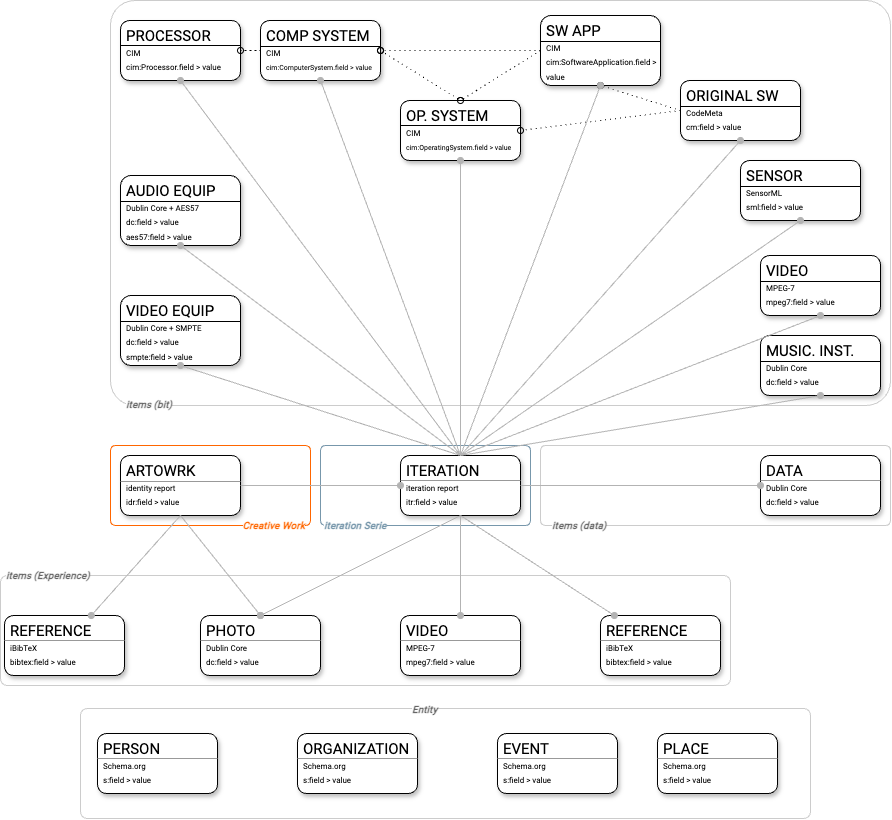
\includegraphics[width=\linewidth]{chapters/4-MDC_model_application/image/graph04-metadata.png}
    \caption{The metadata structure of our MDC Model application according to the metadata scehma introduced above.}
    \label{fig:c4-metadata}
\end{figure}

\section{MDC Model application}

\subsection{Neo4j Graph database application}

The application of the MDC model through the Neo4j graph database is by far the most complex, detailed, and complete case discussed in this text. This system was applied in case studies involving Michele Sambin’s \textit{videoloop} (Appendix~\ref{ax:a-michele_sambin_videoloop}) and Carlo De Pirro’s installation \textit{Il caos delle sfere} (Appendix~\ref{ax:b-hybrid_reactivation_il_caos_delle_sfere}). We will mainly focus on the case study of the \textit{videoloop}, as it presents a highly detailed case with intricate relationships between the various iterations of the artwork, as well as a large amount of documentation created before and during the reactivations.\\
As mentioned several times, Neo4j is a graph database and belongs to the NoSQL database family, which has gained popularity in the last decade as an alternative to traditional relational databases. It is especially useful for managing large volumes of interconnected data, enabling effective storage and retrieval \cite{lourencco2015choosing}. One of the main advantages of Graph databases is their efficiency in handling relationships between data, which were more challenging to manage in traditional relational databases. For this reason, graph databases are increasingly used in the context of social media.\\
Graph databases are easy to understand because their concept is based on graph theory, which is also one of the most useful structures for modelling objects and interactions. Graphs are mathematical structures used to model relationships between objects. In this context, graphs are defined by nodes (or vertices), edges (the relationships connecting the nodes), and properties representing information related to both the nodes and the edges \cite{guia2017graph}. In addition to being intuitive due to their natural representation of information (the graph), graph databases offer many other advantages that are highly relevant to our application context. First, they are much more flexible than relational databases, a characteristic common to all NoSQL databases. They are naturally additive, allowing us to add new types of data, such as nodes or relationships, easily without disrupting the overall structure and functionality of the application. The additive nature of graphs also means fewer migrations, which reduces maintenance overhead and risk.\\
Unlike relational databases and general NoSQL systems, graph databases store data as connected data, with nodes and edges at the same level. Relationships are ``first-class citizens'' of the graph data model, unlike other database management systems that require us to infer connections between entities using properties like foreign keys or out-of-band processing such as map-reduce. The connected data makes creating and querying relationships extremely agile and efficient, naturally enabling path formation. Moreover, relationships are not just links; they have direction and properties that straightforwardly allow us to define the semantic context of the paths. Therefore, graph databases are excellent for data mining operations \cite{robinson2013graph}.\\
Without considering all the computational performance advantages — also defined by the query languages implemented — compared to other types of databases \cite{vicknair2010comparison, guia2017graph, fernandes2018graph}, it is clear that graph databases can be highly efficient for both storing and retrieving information related to live media artworks. As discussed in Chapter~\ref{ch:1-state_of_the_art} and ~\ref{ch:2-new_conservation_paradigms}, one of the main features of live media art is its formal and material heterogeneity, as well as its relational heterogeneity with all the entities and elements it interacts with (the interdisciplinarity of the involved figures, the different types and spaces of exhibition, etc.). Representing this heterogeneity is undoubtedly enhanced by the flexibility offered by graph databases, where we can have a malleable data structure with the simplicity of adding new data structures for nodes and new types of relationships. Moreover, we must consider the complex relationships often found in live media art, including the intricate network of people involved in the artistic project, the exhibition, curation, and conservation of the works. The relationships intensify when we consider the components (\textit{bit}s) used in the works and all the documentation created, which, as seen in Chapter~\ref{ch:2-new_conservation_paradigms}, can trigger a complex network of relationships.\\
Additionally, there are relationships between the works and their iterations. In short, the relationships between elements of a live media artwork are one of the most important aspects in the context of their conservation. The MDC model is built upon this network of relationships, defining multidimensional connections between the artworks and their iterations, between iterations and components and documentation, between iterations and other iterations, and between all elements and the various entities involved (people, organisations, events, etc.). Therefore, the main strength of graph databases — their ability to enhance the relationship structure and derive semantic paths — is the key feature that led us to choose this database for archiving live media art.\\
Neo4j was chosen from many other graph database systems for its positive reviews and popularity. Over the years, this system has been tested and reviewed in both scientific and non-scientific contexts \cite{vicknair2010comparison, robinson2013graph, lourencco2015choosing, guia2017graph, fernandes2018graph, khan2023sql} and has consistently received positive feedback. Additionally, as seen on the DB-Engines website’s Graph DBMS Popularity Trend\footnote{DB-Engines Ranking of Graph DBMS \url{https://db-engines.com/en/ranking/graph+dbms} (last accessed, 19/12/2024)}, Neo4j is currently by far the most popular and fastest-growing graph database.\\
Neo4j is an open-source graph database implemented in Java, first released in 2007. It features its own query language, Cypher, developed by the database's creators, which allows users to manage all the information within the database. Cypher is relatively simple yet very powerful, enabling efficient and expressive query execution and updates to graph databases. Moreover, Neo4j offers an intuitive and user-friendly interface, allowing users to visualise the database as a graph or a JSON table, view all properties for each node and relationship, and quickly enter Cypher commands to work with and query the database.\\
In our application, we use Neo4j to collect all data related to the artworks and their documentation and, most importantly, to create all the relationships. We store all the files associated with artworks, such as source codes, videos, photos, instructions, scores, and so on, in a cloud system (Google Drive) and repositories (GitHub repository). The Neo4j database refers to each multimedia source through URLs.\\
In the following pages, we will explore Neo4j's use and potential in relation to the MDC model.\\
\newline
The first thing to mention is the creation of nodes and relationships. One main feature is that nodes and relationships can be labelled. The label is crucial because we use it to define the type of item and relationship. We could create a node with the label \texttt{CREATIVE\_WORK}, representing the artwork. This node can be easily created as follows:
\begin{lstlisting}[style=cypher]
CREATE (a:CREATIVE_WORK)
\end{lstlisting}
However, we need to assign all the properties of the artwork, which the metadata schema of the identity report will define.
\begin{lstlisting}[style=cypher]
CREATE (a:CREATIVE_WORK
{
       title: 'Il tempo consuma',
       dateCreated: date('1978'),
       description: '...',
       conservationStatement: '...'
}
)
\end{lstlisting}
In this way, we will create the node for the artwork \textit{Il tempo consuma} by Michele Sambin, as shown in Figure~\ref{fig:c4-neo4j-creativework}.
\begin{figure}[!h]
    \centering
    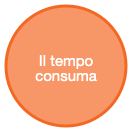
\includegraphics[width=0.165\linewidth]{chapters/4-MDC_model_application/image/neo4j-singlenode.png}
    \caption{Michele Sambin's artwork \textit{Il tempo consuma} neo4j node.}
    \label{fig:c4-neo4j-creativework}
\end{figure}
However, if we refer to the \textit{Identity Report} metadata schema (Table~\ref{tab:c4-artwork}), we don’t see the \textit{artist}, \textit{photo}, \textit{iterationSeries}, and \textit{bibliographySeries} fields in this node\footnote{The \textit{id} field is automatically created by Neo4j when the node is created}. As we’ve seen in the metadata schema, these fields refer to other metadata schemas and, thus, other items. They can be added through relationships.\\
Assuming we’ve already added a \textit{Person} node for Michele Sambin, we can add the relationship artist with the following Cypher query:
\begin{lstlisting}[style=cypher]
MATCH (a:CREATIVE_WORK {title: 'Il tempo consuma'}), (p:PERSON {familyName: 'Sambin'})
CREATE (a)-[r:ARTIST]->(p)
\end{lstlisting}
In this case, we used the \texttt{MATCH} command to select the nodes representing \textit{Il tempo consuma} and \textit{Michele Sambin}. Then, we created a simple directional relationship from the artwork to the person, with \textit{artist} as a metadata field of the \textt{CREATIVE\_WORK} node. We can visualise this, as shown in Figure~\ref{fig:c4-neo4j-artworkrelation}.

\begin{figure}[!h]
    \centering
    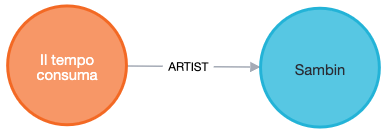
\includegraphics[width=0.5\linewidth]{chapters/4-MDC_model_application/image/neo4j-singlerelationship.png}
    \caption{The relationship between \texttt{CREATIVE\_WORK} and \texttt{PERSON} nodes through the \textit{artist} field of the \textit{Creative Work} metadata scehma.}
    \label{fig:c4-neo4j-artworkrelation}
\end{figure}

Figure~\ref{fig:c4-neo4j-artworkrelation} shows all the first-level relationships of the artwork Il tempo consuma, including the iterations, bibliography, and representative photo.
\begin{figure}[!h]
    \centering
    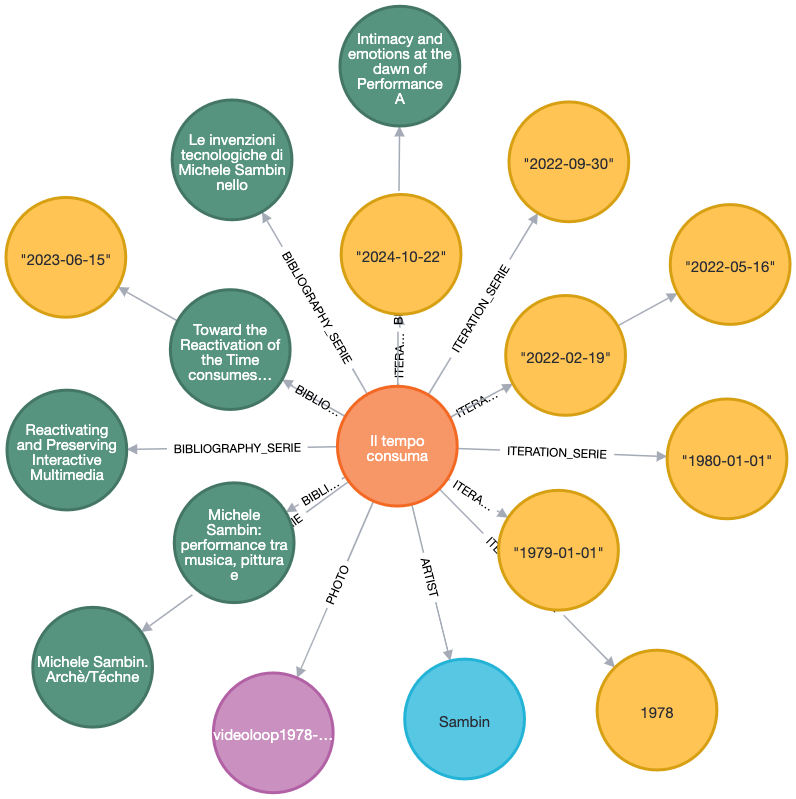
\includegraphics[width=1\linewidth]{chapters/4-MDC_model_application/image/neo4j-artworkrelation.png}
    \caption{First-level Neo4j relationships of \textit{Il tempo consuma} by Michele Sambin.}
    \label{fig:c4-neo4j-artworkrelation}
\end{figure}
One of the features of Neo4j that is very useful in our application context is that relationships can be more than just simple connections; they can also contain properties. With these properties, we can enhance the information about specific relationships. For example, the relationship \texttt{BIBLIOGRAPHY\_SERIE} between \textit{Il tempo consuma} and the monograph \textit{Michele Sambin: performance tra musica, pittura e video} \cite{lischi2014michele} can be expanded by specifying the pages where the authors discuss the \textit{videoloop} topic. The relationship would look like this (in JSON format):
\begin{lstlisting}[style=json]
{"start":0, "end":12, "type": 'BIBLIOGRAPHY_SERIE', "properties": {"pages": ['117-122', '252']}
\end{lstlisting}
So, the relationship between node 0 (\textit{Il tempo consuma}) and node 12 (the monograph)\footnote{Node numbering in Neo4j is based on the order in which nodes are created. Each node is assigned a unique identifier (ID) that reflects its creation sequence.} is of type \texttt{BIBLIOGRAPHY\_SERIE} and can be found in two sections, one on page 117 and the other on page 252.\\
Another very useful case for utilising this feature is the characterisation of performers. One of the iterations of the \textit{videoloop} reactivation was performed by multiple people, in addition to Michele Sambin and the author of this text (usually video and audio director), as is typical in the performance of the digitalised version of the \textit{videoloop}. In Figure~\ref{fig:c4-neo4j-performer}, we can see all the performers of the performance at the Sala dei Giganti in Padua on 16 May 2022, during the \textit{Opera Libera} event, part of the celebrations for the 800th anniversary of the University of Padua.
\begin{figure}[!h]
    \centering
    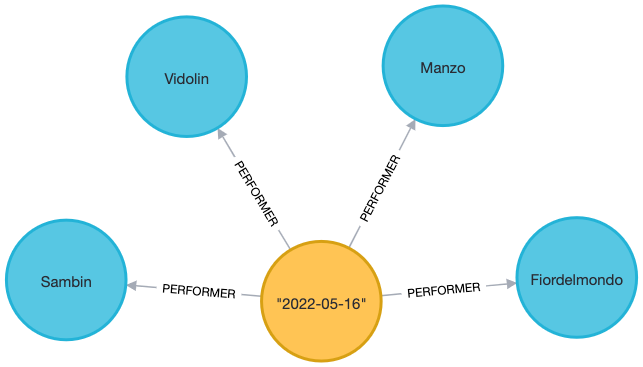
\includegraphics[width=0.75\linewidth]{chapters/4-MDC_model_application/image/neo4j-performer.png}
    \caption{Performers of one of the iteration of the digital version of \textit{Il tempo consuma}.}
    \label{fig:c4-neo4j-performer}
\end{figure}
At this point, we only see the relationship as \texttt{PERFORMER}, but we don’t know more about each person's role in the performance, so they all appear at the same level. However, if we click on the individual relationships, we can see all the properties and further characterise them:
\begin{lstlisting}[style=json]
"start": 6, "end": 1, "type": 'PERFORMER',  "properties": {“performerAs”:'main performer', “note”: '...'}
"start": 6, "end": 17, "type": 'PERFORMER',  "properties": {“performerAs”:'video director', note”: '...'}
"start": 6, "end": 18, "type": 'PERFORMER',  "properties": {“performerAs”:'vocal performer', “note”: '...'}
"start": 6, "end": 19, "type": 'PERFORMER',  "properties": {“performerAs”:'sound director', “note”: '...'}
\end{lstlisting}
This capability is one of Neo4j's main features: it allows us to treat relationships at the same level as nodes and with the same capabilities. Of course, this is very useful in our case, as it significantly enriches the information about an artwork and, in this specific case, the details of a performance. Moreover, this feature extends across the entire network of interactions surrounding the artwork, thus enhancing the information about each entity (\textit{actant}) involved in the \textit{ecological turn} discussed in Chapter~\ref{ch:2-new_conservation_paradigms}.\\
In Figure~\ref{fig:c4-neo4j-artworkrelation}, we saw the relation between the MDC model's first and second levels, respectively, the artwork and iterations level. Now, we can dive deeper into the details of the Iteration file, thus examining the lowest level of items, i.e. \textit{bit}s, \textit{data} and \textit{experience}, in relation to a single iteration of the artwork. Figure~\ref{fig:c4-neo4j-iteration} shows the first iteration of the digitally reactivated \textit{videoloop}, performed at the Costromediano Museum in Lecce on February 19, 2022.

\begin{figure}[!h]
    \centering
    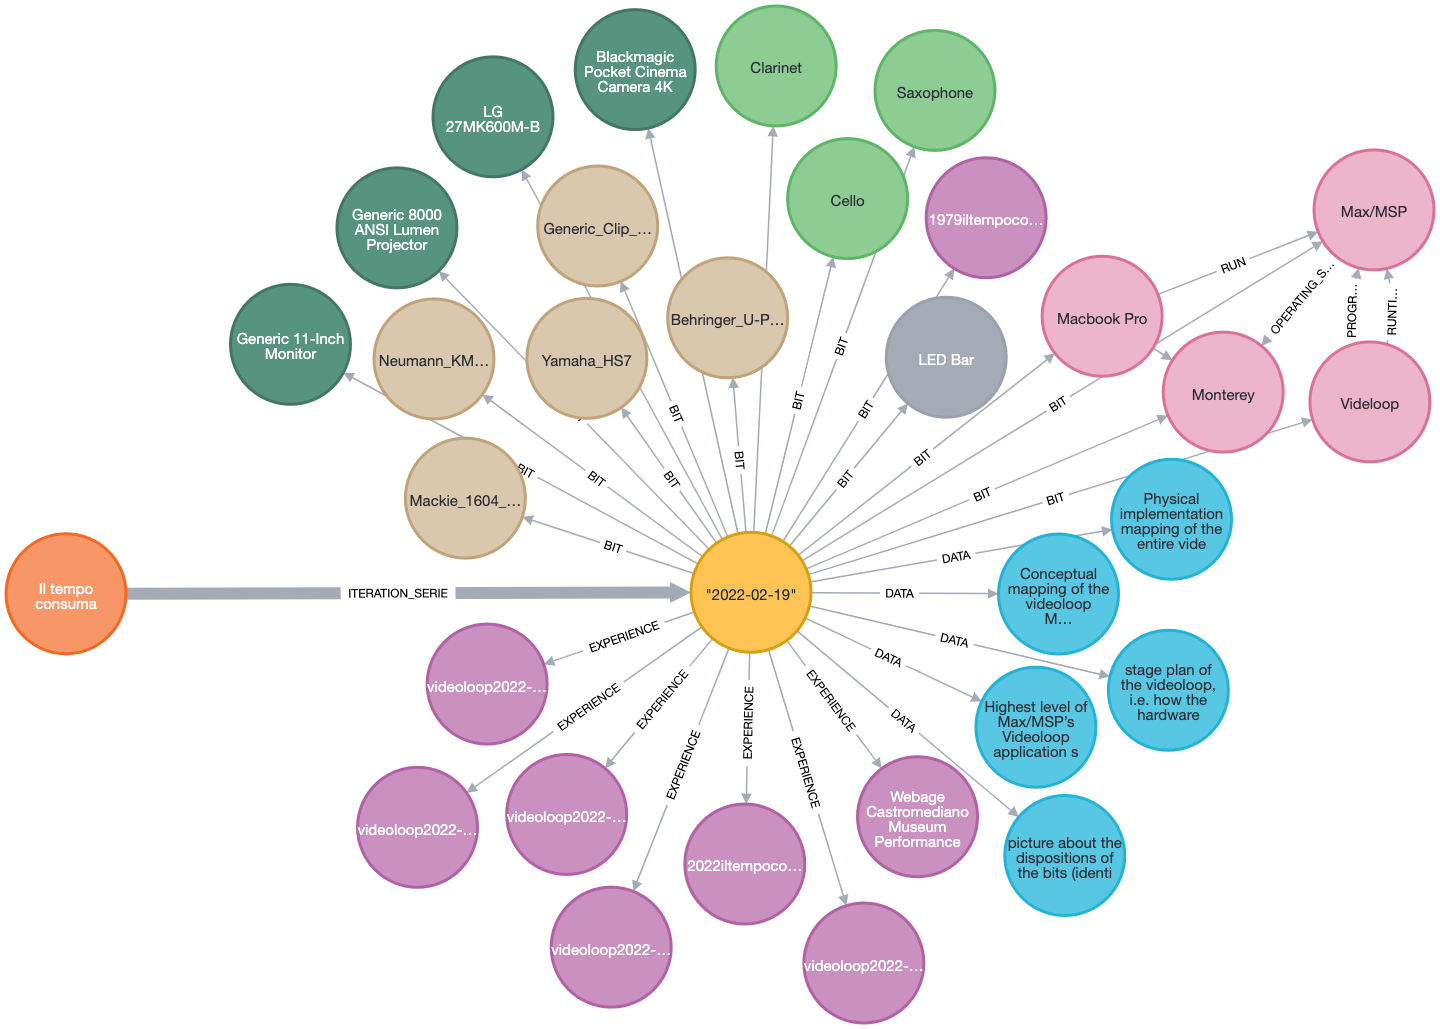
\includegraphics[width=1\linewidth]{chapters/4-MDC_model_application/image/neo4j-iteration.png}
    \caption{The relationship of an \textit{Il tempo consuma}'s iteration with \textit{bit}s, \textit{data}, and \textit{experience}.}
    \label{fig:c4-neo4j-iteration}
\end{figure}

At this level, we can see all the \textit{bit}s, such as audio components, video, hardware, and software used\footnote{In Figure~\ref{fig:c4-neo4j-iteration}, it is also possible to see the relationships between the \textit{bit}s representing the computer, operating system, and software. These relationships are enabled by the \textit{Common Information Model} (CIM), which is defined as part of the metadata standard.}; the various \textit{data}, which include all the modules and mappings related to the MIF and BVL application discussed in Chapter~\ref{ch:3-mdc_model-reactivation_workflow-instruction_template}; and finally all the experiences and the documentation created, such as a documentary video, photos, and a webpage related to the performance\footnote{In Figure~\ref{fig:c4-neo4j-iteration}, the number of collected \textit{experience}s has been significantly reduced to better visualize the database, especially in relation to other types of items.}. Therefore, when considering the MDC model, Figures~\ref{fig:c4-neo4j-artworkrelation} and ~\ref{fig:c4-neo4j-iteration} show us the \textit{multilayering} property of the model applied through Neo4j.\\
However, we still need to visualise another important property of the MDC model: \textit{multiple belongingness}. We can easily create and display this property thanks to Neo4j’s system of relationships and queries. The \textit{videoloop} case study also provides many interesting examples of \textit{multiple belongingness} in practice.\\
First, let’s start with the most superficial relationships of \textit{multiple belongingness}, which can be found at the level of \textit{bit}s and \textit{data}, such as items that belong to more than one iteration. In the context of Neo4j, we only need to create the \textit{bit} or \textit{data} item once and then create a relationship for each iteration. To visualise the relationship through Cypher, we simply need to query the database to determine which iterations use that specific item.\\
\begin{lstlisting}[style=cypher]
MATCH (i:ITERATION)-[:BIT]->(a:AUDIO_EQUIPMENT {identifier: "Behringer_U-Phoria_UMC204HD"})
\end{lstlisting}
With this simple command, we ask the database which iterations use the Behringer U-Phoria UMC204HD audio interface as a \texttt{BIT} relationship. The output is shown in Figure~\ref{fig:c4-neo4j-multiplebel01}.

\begin{figure}[!h]
    \centering
    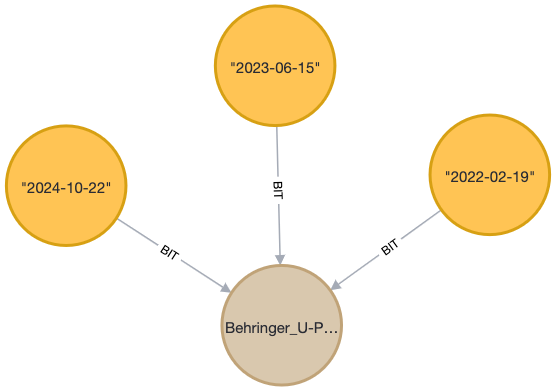
\includegraphics[width=0.5\linewidth]{chapters/4-MDC_model_application/image/neo4j-multiplebel01.png}
    \caption{\textit{Multiple Belongingness} for the audio interface Behringer U-Phoria UMC204HD in Neo4j.}
    \label{fig:c4-neo4j-multiplebel01}
\end{figure}

As we can read from the output, three iterations use this specific audio interface.\\
When analysing this artwork, another very interesting example is the usage of mappings, especially \textit{Conceptual Mapping}. As defined in Appendix~\ref{ax:a-michele_sambin_videoloop}, related to this case study, \textit{Conceptual Mapping} is the common element across all iterations, both from the 1970s and those reactivated in the digital domain. However, if we don’t already know this information, we can ask the database to find the common elements across all iterations. This kind of information can be useful for understanding whether there is a recurring element across all the iterations that could, in specific analysis, be defined as a critical element of the artwork’s identity.\\
To obtain this information, we must write a more ``complex'' Cypher query, which is still very short. First, we must match all relationships between the iteration nodes and other nodes (items). Indeed, we need to select those relationships that start from the iteration, i.e. directional relationships from the iteration to the item level (otherwise, we would obtain the artwork as common nodes).
\begin{lstlisting}[style=cypher]
MATCH (i:ITERATION)-[r]->(n)
\end{lstlisting}
Then, we must create a list aggregating all the nodes found for each iteration.
\begin{lstlisting}[style=cypher]
WITH i, COLLECT(n) AS relatedNodes
\end{lstlisting}
So, for each \texttt{ITERATION} (\texttt{i}), we will collect the related nodes (\texttt{n}), resulting in a structure like the table~\ref{tab:c4-neo4jtable01}:

\begin{table}[!h]
    \centering
    \begin{tabular}{|c|c|}
    \hline
        \textbf{\texttt{i}}  & \textbf{\texttt{relatedNodes}} \\ \hline
         1          & \texttt{[n1, n2, n3, ...]} \\ \hline
         2          & \texttt{[n3, n5, ...]} \\ \hline
         3          & \texttt{[n1, n3, n6, n7, ...]} \\ \hline
         ...          & ... \\ \hline
    \end{tabular}
    \caption{Node connected to each iteration.}
    \label{tab:c4-neo4jtable01}
\end{table}
Then, we use a series of commands to find the common nodes across the different lists (e.g., in the table above, this would be \texttt{n3}).
\begin{lstlisting}[style=cypher]
WITH COLLECT(relatedNodes) AS allRelatedNodes
WITH REDUCE(common = HEAD(allRelatedNodes), current IN TAIL(allRelatedNodes) |
    [node IN common WHERE node IN current]) AS commonNodes
\end{lstlisting}
Using the \texttt{COLLECT} command, we group all the lists of nodes from individual iterations into a single ``list of lists,'' structured as \texttt{allRelatedNodes = [[n1, n2, n3], [n3, n5], [n1, n3, n6, n7], …]}. Then, we reduce (\texttt{REDUCE}) this list to keep only the nodes that appear in every sublist. Step by step, we start with the first sublist in \texttt{allRelatedNodes} and compare it with the rest of the sublists one by one, using the commands \texttt{HEAD} (to get the first sublist) and \texttt{TAIL} (to get the remaining sublists). For each comparison, we check which nodes are shared between the current ``common'' nodes and the next sublist using \texttt{[node IN common WHERE node IN current]}. Once we’ve compared all the sublists, we get a final list of nodes shared across all sublists saved as \texttt{commonNodes}.\\
In our case, as mentioned earlier, we get the graph shown in Figure~\ref{fig:c4-neo4j-multiplebel02}.

\begin{figure}[!h]
    \centering
    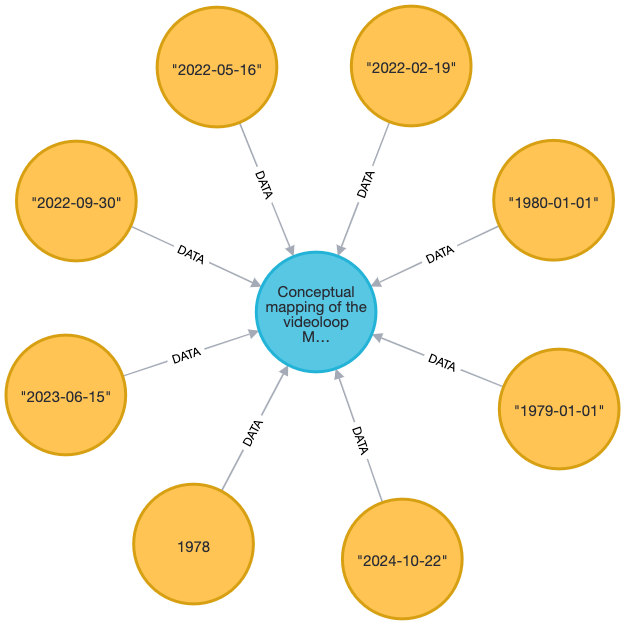
\includegraphics[width=0.75\linewidth]{chapters/4-MDC_model_application/image/neo4j-multiplebel02.png}
    \caption{Result of the search for the node common to all iterations. By querying the Neo4j database of ‘il tempo consuma’ by michele sambin (structured according to MDC) we found the concept mapping as a fixed element between iterations. This is possible due to the \textit{multiple belongingness} property of the MDC model.}
    \label{fig:c4-neo4j-multiplebel02}
\end{figure}

We can go quite far with the search for \textit{multiple belongingness}, especially in this case study. For example, we can see how an item can have two different functions for two different iterations. The video produced for the \textit{Il tempo consuma} performance in 1979 documents the same performance and is therefore classified as an \textit{experience}. However, as shown in Appendix~\ref{ax:a-michele_sambin_videoloop}, the same video is used as the introduction to the digital \textit{videoloop} performance. The digital performance of the \textit{videoloop} begins with this video recording, which dissolves into the present live performance (transitioning from the young Michele Sambin of 1979 to the present one, emphasising the time-consuming theme). So, in the reactivated versions, the video recording is considered a \textit{bit}, as shown in Figure~\ref{fig:c4-neo4j-expbit}.
\begin{figure}[!h]
    \centering
    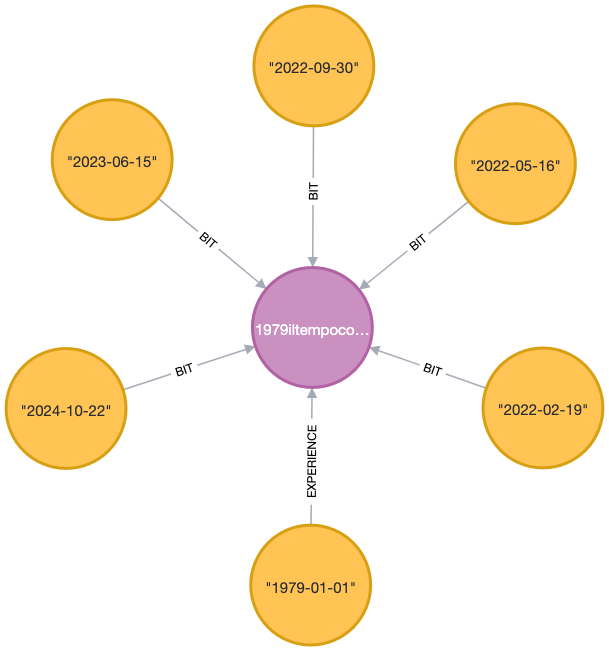
\includegraphics[width=0.75\linewidth]{chapters/4-MDC_model_application/image/neo4j-expbit.png}
    \caption{According to the \textit{Multiple Belongingness}, the same item can be associated with different iterations, each serving a different function. In this case, the \textit{videoloop} video recording remains as an \textit{experience} in one performance, while acting as a \textit{bit} in the digitally reactivated iterations.}
    \label{fig:c4-neo4j-expbit}
\end{figure}
This case is an example of reused documentation as an artistic element (documentation \textit{as art}), which we discussed in Chapter~\ref{ch:2-new_conservation_paradigms}. And this is also why, within Neo4j, we do not define items as \textit{bit}s, \textit{data}, or \textit{experiences}. Instead, we define them as items with characteristics independent of the conservation model, such as simple devices, mappings, photos, videos, etc. The quality that defines the item in the context of the MDC model—i.e., \textit{bit}, \textit{data}, and \textit{experience}—is determined by the relationship with the iteration.\\
As defined in Chapter~\ref{ch:3-mdc_model-reactivation_workflow-instruction_template}, the property of \textit{multiple belongingness} can occur not only at the lowest level of the model but also at the series level. The \textit{videoloop} is a very interesting case from this perspective because, in the reactivated versions, a series of different works are performed, not just \textit{Il tempo consuma} (see Appendix~\ref{ax:a-michele_sambin_videoloop} for more information). Therefore, if we take an iteration from the reactivations, for example, the first one in 2022 at the Castromediano Museum in Lecce, we can see that this iteration belongs to more than one artwork. In Figure~\ref{fig:c4-neo4j-multipleartworks}, we can see the \textit{multiple belongingness} of an iteration in relation to the artworks.

\begin{figure}[!h]
    \centering
    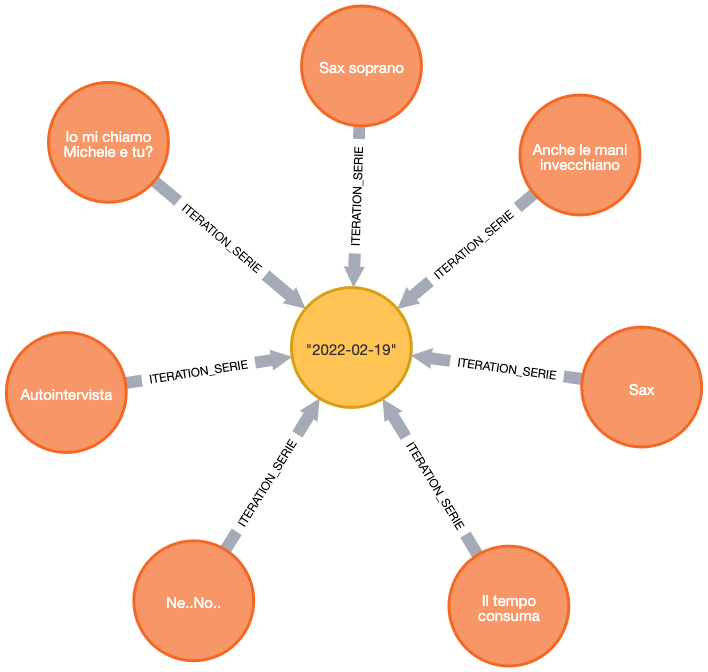
\includegraphics[width=0.75\linewidth]{chapters/4-MDC_model_application/image/neo4j-multipleartwork.png}
    \caption{According to the \textit{multiple belongingness}, even a single iteration can be associated with multiple artworks. This graph illustrates a Neo4j example of the reactivated \textit{videoloop}, where other pieces (beyond just Il tempo consuma) are performed in sequence (refer to Appendix~\ref{ax:a-michele_sambin_videoloop} for more information)}.
    \label{fig:c4-neo4j-multipleartworks}
\end{figure}

Finally, We can also see the relationship between archived artworks (i.e. those by different authors). For example, we can see the artworks exhibited in a specific event. In our case, we have an example that links the \textit{videoloop} to another reactivated artwork, \textit{Il caos delle sfere}. During the Science4all event on 30 October 2022 in Padua, both works were exhibited (the \textit{videoloop} as an installation) in the same space. In Figure~\ref{fig:c4-neo4j-event}, we can see the relationship between the two artworks through the event.

\begin{figure}[!h]
    \centering
    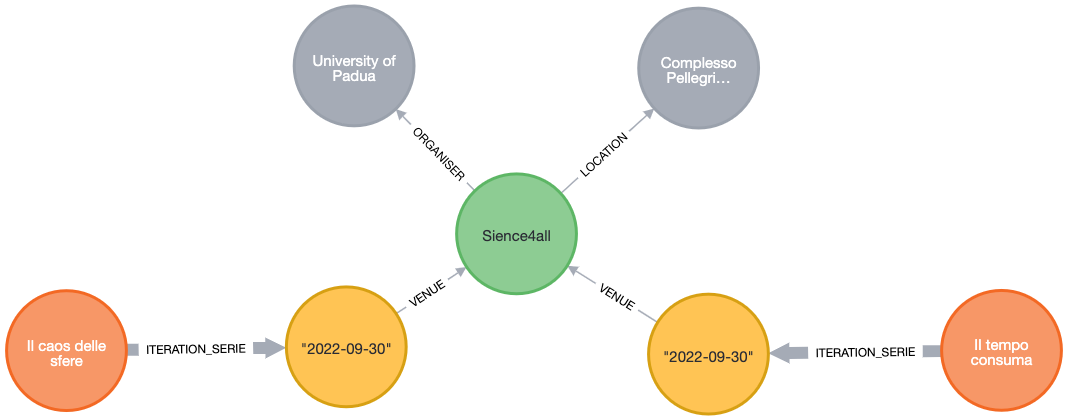
\includegraphics[width=\linewidth]{chapters/4-MDC_model_application/image/neo4j-event.png}
    \caption{Relationship between two archived artworks in the Neo4j database. The connection is traced through the reactivation of \textit{videoloop} and the installation \textit{Il caso delle sfere}, which were presented together in the same event.}
    \label{fig:c4-neo4j-event}
\end{figure}

These are just a few simple examples, but they are also very relevant in showcasing the potential of Neo4j, its Cypher query language, and the design of the MDC model in relation to this graph database.\\
The database can be used in various ways, from its use on the web, such as in an online archive, to desktop applications for both archiving and generating descriptive sheets for artworks. For example, in our case, we developed a simple Python application that can create both identity reports, similar to those used by museums, and technical sheets for further reactivations of the artwork. 

\subsection{GitHub Repositories application}
Another application of the MDC model is through GitHub. As mentioned, GitHub is a popular web-based platform for version control and collaborative software development. It is built on Git, a distributed \textit{Version Control System} (VCS) that allows developers to track changes, manage projects, and collaborate on both open-source and private software. Git works with repositories—storage locations used to collect and manage data. One key advantage of Git compared to other VCSs is its ability to preserve a complete repository copy with full history and version tracking. Today, Git is the standard among existing VCSs, and GitHub and GitLab are the primary platforms for its use.\\
As previously discussed in this chapter and Appendix~\ref{ax:d-sustainability_and_longevity_of_nimes}, we chose to test this development platform because it is widely used in various research projects, not only scientific ones but also increasingly in artistic and creative projects. For example, it is often used in the aforementioned context of New Interfaces for Musical Expression (NIME), which is a highly interdisciplinary field combining both scientific and artistic research.\\
We applied the MDC model for archiving and documenting two NIMEs: \textit{Soundrise}, a multimedia application developed by the CSC, and \textit{Electronic\_Khipu\_} and \textit{Kanchay\_Yupana}, two complementary digital musical instruments (DMIs) created by Patricia Cadavid, a Colombian musician and researcher.\\
Before diving into the application of the MDC model in this context, some clarifications are needed. First, it is essential to emphasise that GitHub is not an archival tool. While it does have some potential for archival purposes, especially for preserving source code, tracking versions, and similar tasks, it is not specifically designed for this function. Instead, GitHub complements archival systems. For example, in the context of the Neo4j archive, GitHub could support the archiving of original software developed for the artworks. However, it is unlikely to function effectively as a standalone archival system.\\
GitHub is primarily a development tool. Its version tracking and file preservation features are aimed more at analysis, bug tracking, problem-solving, and collaborating on changes rather than long-term archiving. For instance, one key difference between GitHub and a traditional museum archive is their focus. Museum archives typically prioritise documenting the ``original'' version of an item, while GitHub (and software development in general) focuses on the ``latest version.''\\
Our specific application does not perfectly align with either case. We have moved beyond the idea of an ``original'' work, and we cannot focus solely on the ``latest version.'' Instead, we need to consider the entire set of versions. Thus, we need to adapt the design of a GitHub repository to fit the MDC model.\\
Another important aspect that differs from the Neo4j application is that GitHub is more like a ``cloud platform'' for storing files while Neo4j is just a database designed to store and manage data and could be integrated with cloud services. Although GitHub is better suited for storing source code files and text, it can also store images, audio, and videos. However, videos and large files (limited to 2GB for the free plane) cannot be directly viewed within GitHub’s web interface.\\
While GitHub lacks a dedicated tool for managing databases like Neo4j, and the case studies where the MDC model has been applied often follow different principles compared to artworks, it is still important to apply the MDC model in this context. Again, GitHub is increasingly being used in multi- and interdisciplinary fields and is more and more popular in the arts, which is why it is important to design the application of the MDC model with it.\\
\newline
A GitHub repository functions as a file storage system and includes an editable front page that serves as documentation. This page can contain textual information, images, and links related to the repository or external sources. The page is created using a \texttt{README.md} file, which works similarly to \texttt{index.html} in web pages. It can be edited using GitHub’s Markdown language (the ``.md'' extension comes from Markdown) and includes basic HTML tags.\\
We can have multiple \texttt{README.md} files, one for each directory, so each directory has its own introductory page. We can also add more \texttt{.md} files to expand the documentation for the repository or specific directories. In practice, when viewing a GitHub repository, we see the directory structure, which is displayed as folders and files, along with the front page. We can navigate through the repository or interact with the front page by reading the documentation and following the provided links.\\
In the main directory, we can also have other important files commonly used in software development and sharing. For example, a \texttt{LICENSE} file specifies the terms under which the project can be used or distributed. For each file, especially text files (such as code files), and excluding larger multimedia files (like videos), we can have specific features for viewing and interacting with the files. For instance, text files can be edited directly within GitHub.\\
The most important feature of a GitHub repository is the VCS, which allows us to track the history and changes made to the repository. Every update creates a \textit{commit}, which we can comment on to describe the changes. A \textit{commit} is a snapshot of the changes made to the repository, helping us track modifications over time. We can also create multiple branches—parallel versions of the repository. In addition to the main development branch, called ``main,'' we can develop several branches for specific development tasks or experimentation. Figure~\ref{fig:c4-github-tree} shows a typical repository development with commits and a tree of branches.

\begin{figure}[!h]
    \centering
    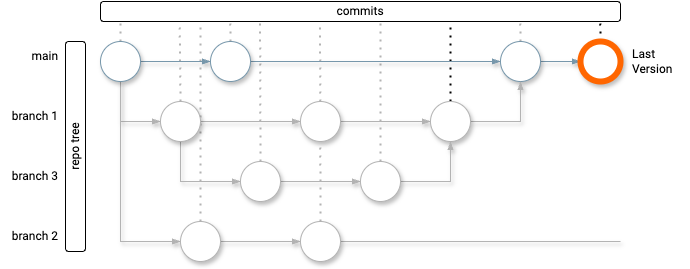
\includegraphics[width=1\linewidth]{chapters/4-MDC_model_application/image/graph04-githubtree.png}
    \caption{VCS repository development tree.}
    \label{fig:c4-github-tree}
\end{figure}

Within the \texttt{README.md} file, we can include links to different versions (based on the repository’s history) and various branches. GitHub also offers many other useful features for software development, such as collaboration tools, \textit{Issues}, \textit{Pull Requests} (PRs), and \textit{Discussions}, as well as automation, settings, and accessibility options. However, in our case, we will focus on GitHub’s essential features, which we will use primarily as a storage system.\\
We created a template repository to demonstrate the ideal application of the MDC model through GitHub. The repository is structured as shown in Figure~\ref{fig:c4-github-template}.

\begin{figure}[!h]
    \centering
    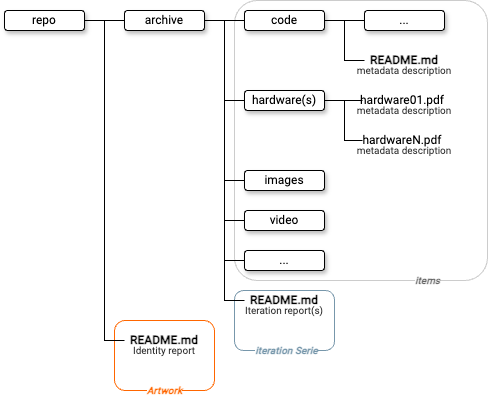
\includegraphics[width=\linewidth]{chapters/4-MDC_model_application/image/graph04-githubtemplate.png}
    \caption{GitHub repository structure template according to the MDC model appilication.}
    \label{fig:c4-github-template}
\end{figure}

The repository's main directory contains two main components: an archive subdirectory and the \texttt{README.md} file. The \texttt{README.md} serves as the general description of the artwork and follows the descriptive fields defined in the \textit{Identity Report} metadata schema. In this case, the \textit{bibliographySeries} field will be filled on the same page as the identity report, while the \textit{iterationSeries} field will refer to the \textit{archive} subdirectory. At this level, we have the highest level of the MDC model, the \textit{Creative Work} level.\\
Within the \textit{archive} subdirectory, we have additional subdirectories and, again, another \texttt{README.md}. This \texttt{README.md} will represent the \textit{Iteration Series}, which will be filled out using the \textit{Iteration Report} metadata schema. Each iteration will have a table with the main information about the iteration, followed by a set of details. The details will include \textit{bit}s, \textit{data}, and \textit{experience}. For \textit{bit}s (component list), we will use simple fields like \textit{type} (e.g., computer system, software, audiovisual), \textit{name}, \textit{version} (optional), \textit{link} (internal or external), \textit{requirements} (optional), and \textit{notes} (optional). The \textit{data} section (technical notes, mapping, and instructions) will include text and images, ideally following the instruction template defined in Chapter~\ref{ch:3-mdc_model-reactivation_workflow-instruction_template}. Finally, the \textit{experience} section (documentation) will contain photos, videos, and links to external or internal files. Figure~\ref{fig:c4-github-template02} is a schematic of the archive’s \texttt{README.md} file.

\begin{figure}[!h]
    \centering
    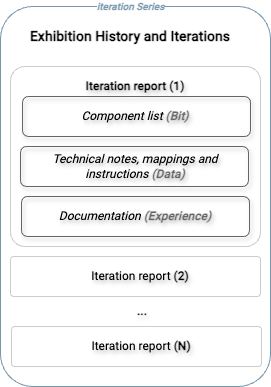
\includegraphics[width=0.4\linewidth]{chapters/4-MDC_model_application/image/graph04-githubtemplate02.png}
    \caption{GitHub repository structure template according to the MDC model appilication. Structure of the archive's \texttt{README.md} with the \textit{Creative Work}'s iterations}
    \label{fig:c4-github-template02}
\end{figure}

The subdirectories within the \textit{archive} will contain all the files related to the artwork, such as images, videos, source code, and hardware components. Following the Neo4j application approach, we do not separate \textit{bit}s, \textit{data}, and \textit{experience} at the storage level since the same item might be used differently across different iterations. The classification of an item as a \textit{bit}, \textit{data}, or \textit{experience} occurs at the iteration description level. Each item should have a proper description compiled. For source code, for example, we could have a folder containing all directories related to the specific code, organised by programming language, system used, and developer. However, here, in the main directory for the source code, we could use the \texttt{README.md} file to compile the metadata description. In other cases, such as for hardware, we could use PDFs or text files (ranging from a simple \texttt{.txt} to more specific formats like \texttt{JSON}) to compile the metadata for the specific hardware item (an example, in the template repository, is the PDF of the mechanical arm).\\
So far, we have described the hierarchical structure of the MDC model applied to a GitHub repository. Applying \textit{multiple belongingness} in this context is less effective than in Neo4j; however, it still has its potential, especially in some instances. Firstly, GitHub does not have a built-in feature to show all the pages or files directly where a specific file is referenced within a repository. This means we cannot quickly and clearly visualise \textit{multiple belongingness} as we could in Neo4j. Instead, we can only create links in the \textit{iteration series} to refer to a specific file for each iteration. This can be seen in the \textit{iteration series}’ components list under the \textit{link} field in the table. However, here, we can take advantage of one of Git’s main features: the history and branches of the repository. In the same repository, for each release of a code or specific version (for which we can create branches), direct references are automatically created, and they can be tracked. In the \texttt{README.md} files, we can refer to each step and path of the code, specifically to each commit. This allows us to avoid creating multiple copies of the same file for different versions, and instead, we can simply reference it using Git commits.\\
Below is a simple example of using this in the \textit{mdc-template} repository.\\
We start by adding the final version of the software to the repository, which will be used in the first iteration of the artwork. This action can be done through the web interface or via terminal commands. The terminal commands will look like this:
\begin{lstlisting}[style=bash]
$ git add archive/firmaware                   # add the firmware directory to the repo
$ git commit -m “firmaware-release-v1.0.0”    # commit the action as the new release
$ git commit push                             # push the new file in GitHub repo
\end{lstlisting}
The reference link used in the first and only iteration described in the README.md will be:
\begin{lstlisting}[style=markdown]
<!-- [name link](/path/to/the/folder) -->
[repo link](firmware)                          # push the new file in GitHub repo
\end{lstlisting}
Since the \texttt{README.md} and the firmware directory are in the same archive directory, we only need to enter the firmware folder. After developing a new version of the firmware, we would repeat the process and upload the latest release. This time, the commit would be:
\begin{lstlisting}[style=bash]
$ git commit -m “firmaware-release-v2.0.0”     # commit the new file in GitHub repo
\end{lstlisting}
The new iteration described in the \texttt{README.md} will have the same link as before, pointing to the latest release in the firmware directory. However, the link will change from the first release to:
\begin{lstlisting}[style=markdown]
<!-- [name link](https://github.com/example-user/repository/commit/commit_hash) -->
[commit link] (https://github.com/user/mdc-template/commit/255c12bfb5746cbc1978f076ae05f1f10b72bb51)
\end{lstlisting}
This link refers to the repository's main directory: \texttt{github.com/user/mdc-template/}. We search for a specific \textit{commit} using its hash (``commit\_hash''), which is an identifier string (e.g., \texttt{c4d2a03}). Clicking on the link will take us to the files from the first firmware version.\\
If we want to access the entire release history (and all firmware commits), we can go to the firmware’s main directory. On this page, above the \texttt{README.md} and the root of the folder, we can access the ``History'' section. Inside the History page of a specific folder or file, we can see the list of commits with their corresponding hashes. We can access different branches in the repository's main directory. Under the repository name, we can view and select different branches.\\
\newline
This application is a basic GitHub application that fits the MDC model. Of course, it can be extended to other use cases by utilising various features and capabilities of Git and GitHub.\\
We have adopted and adapted this template for the case studies introduced in Appendix~\ref{ax:d-sustainability_and_longevity_of_nimes}.\\
The \textit{Soundrise} repository was developed as a historical archive for the application and closely follows the GitHub template structure described earlier. However, there are slight differences. In this case, we are not dealing with an artwork but a web application (originally a desktop one). This difference required revising the descriptive fields (no longer the \textit{Identity Report} fields), which is the main modification compared to the template. Other changes were made, but they are of little significance (e.g., the \texttt{README.md} in the main directory includes a \textit{Technical Notes} section, as the technical aspect of the web application is essential).\\
The repository for Patricia Cadavid’s DMIs is more distant from the template. In this case, the repository’s purpose is not strictly archival but instead focused on longevity, replicability, and the continuation of the DMI. We adapted the template to a more development-oriented approach, making it more appropriate for a GitHub repository. The first revision involved removing the \textit{archive} directory, and all software and hardware components were placed in the main directory for easier access. In the same main directory, we created a documentation folder to store all video and audio documentation, as well as two other essential folders: \textit{instructions} and \textit{old\_versions}. Since the repository is focused on replicability and the continuation of the instrument, the \textit{instructions} folder (containing details about how to build the instrument) plays a central role. The \textit{old\_versions} folder contains previous iterations of the instrument. Figure~\ref{fig:c4-github-template03} shows the directory structure for Patricia Cadavid’s instruments repository.

\begin{figure}[!h]
    \centering
    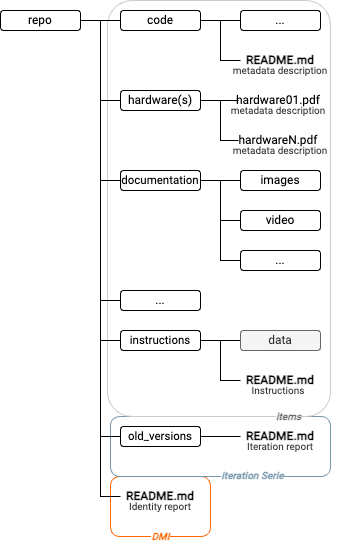
\includegraphics[width=0.75\linewidth]{chapters/4-MDC_model_application/image/graph04-github-template03.png}
    \caption{GitHub repository structure for Patricia Cadavid's digital musical instrument.}
    \label{fig:c4-github-template03}
\end{figure}

Although somewhat intricate, we have seen that the MDC model can also be applied in the context of GitHub. However, Git and GitHub are particularly suited for project development and less adaptable for archival purposes, especially when storing numerous multimedia files. For archival needs and extracting data with complex relationships, Neo4j is undoubtedly a more suitable tool. That said, in more complex and comprehensive contexts, combining Neo4j and GitHub (along with a storage system for multimedia files) creates a robust solution for implementing the MDC model. For instance, consider the DMIs developed by Cadavid. Installations or performances that use these DMIs in conjunction with other devices, multimedia files, etc., could be archived using a Neo4j database. Neo4j nodes could represent the DMIs (as \textit{bit}s) and link directly to their GitHub repositories. The GitHub repositories would contain all information about the DMIs and their development. Neo4j nodes could reference previous versions of the DMIs simply by linking to GitHub \textit{commit}s. This approach would create an interesting hierarchical relationship between two MDC archives, effectively representing the complexity of live media art projects.

\subsection{Finder management system application}
In contrast to the complexity and effectiveness of combining Neo4j and GitHub, we present the simplest and most basic application of the MDC model: using Apple’s Finder. While this method is the least likely to achieve the ideal and functional structure of the MDC model, the use of Finder (or similar local file management systems) is still crucial. In many situations, it becomes a necessary tool. In our cases, we used Finder before a more structural archiving, during the reactivation process, or for personal archiving of copyrighted works. This scenario often occurs when a work’s ``actor''—such as a performer, collaborator, or developer—needs to archive materials related to their contributions. Due to copyright restrictions, these materials are typically stored on personal computers (or, less frequently, in private cloud repositories). This scenario involves what we call an ``actor’s archive'', where an individual actor maintains a collection of their contributions (e.g., performances, software development, etc.) to enable future reactivations. An example from our work is the reactivation and performance of live electronics pieces discussed in Appendix~\ref{ax:c-the_score_in_live_electronics_music}, particularly \textit{Perseo e Andromeda}. For this piece, we gathered extensive documentation on past versions and performances, including scores, code, audio and video recordings, photos, and more. This documentation was essential for the \textit{Assessment} and \textit{Transcription} phases of the live electronics component of the piece. However, the work is subject to copyright by Ricordi, and the original materials are stored in the Paul Sacher Foundation in Basel and the Archivio Storico Ricordi in Milan. As such, we could not create a public archive; instead, we maintained all documentation locally for future reactivations.\\
When using Finder, it’s important to remember that it is a basic storage system. It only allows us to create directories (folders) and place files within them. Unlike repositories, it does not offer features like presentation pages. However, we can use two key features of Finder: \textit{Aliases} and \textit{Tags}. Figure~\ref{fig:c4-finder} shows how the MDC model can be used to organise directories in a Finder folder.

\begin{figure}[!h]
    \centering
    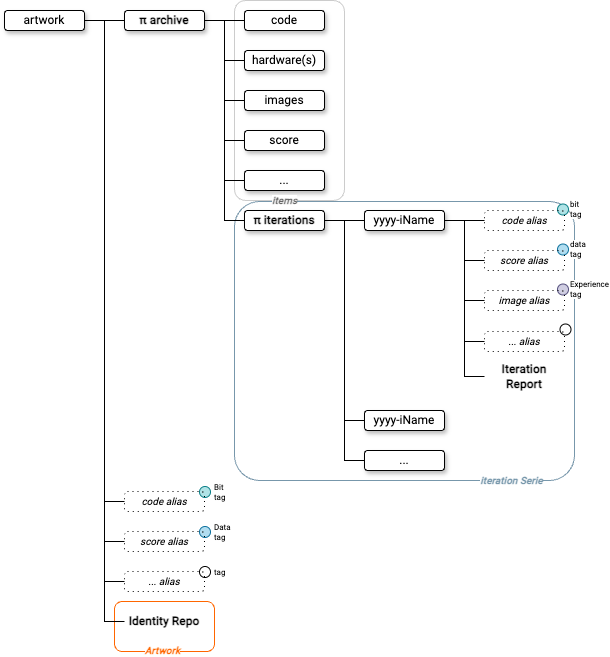
\includegraphics[width=\linewidth]{chapters/4-MDC_model_application/image/graph04-finder.png}
    \caption{A Finder folder organised according to the MDC model, using Aliases (indicated by the dotted boxes) and Tags (represented by the coloured circles in the top-right corners of the boxes).}
    \label{fig:c4-finder}
\end{figure}

This folder organisation was also used to archive \textit{Perseo e Andromeda}. First, the directories' structures are very similar to those shown in Figure~\ref{fig:c4-github-template} (in the context of the GitHub template) and Figure~\ref{fig:c4-github-template03} (in the context of Cadavid’s tool repository). The key similarity is the \textit{archive} folder, which contains all items, such as code, scores, images, videos, etc. Inside the \textit{archive} folder, there is an \textit{iterations} folder (similar to the \textit{old\_version} folder in Cadavid’s repository), where different iterations of the work are grouped into subfolders named \texttt{yyyy-iName} (year and the iteration name). Both of these folders start with the Greek letter $\pi$ (pi). This character is one of the few sorted after ``z'' in Finder’s alphabetical ordering, ensuring that the \textit{archive} and \textit{iterations} folders always appear at the bottom of the list, thus making it easier to find among the other folders.\\
The main differences compared to GitHub are the lack of the \texttt{README.md} file, the use of \textit{aliases}, and the use of \textit{tags}. Instead of \texttt{README.md}, we can use PDFs or text files (\texttt{.txt}, \texttt{.json}, etc.) created specifically for the \textit{Identity} and \textit{Iteration Reports}. However, there is a problem in linking an object to a specific iteration in which it belongs. In Neo4j, we could create direct relationships, while in GitHub, we used links in \texttt{README.md} to reference a specific object in the repository. In Finder, this relationship can be made using \textit{aliases}. An \textit{alias} is a special kind of shortcut that acts as a pointer to the original file or folder. It allows you to access or open the original item from another location without duplicating it. In Finder, you can create multiple \textit{aliases} for a file and place them in the specific iteration folder where that file belongs. Using \textit{aliases} allows us to apply the MDC model’s \textit{multiple belongingness} property.\\
To indicate the type of relationship between the iteration and a specific item, we used the iteration label in Neo4j, while in GitHub, we created a specific table listing all properties in the iteration report. In Finder, we can create and use custom \textit{tags} for files and folders. In our case, we use them only for aliases to indicate the type of relationship between the iteration and the specific alias, which can be \textit{bit}, \textit{data}, or \textit{experience}. Even here, we do not define the item type in the archive but rather its specific use within a single iteration.\\
One last point to note, which is very similar to Cadavid’s DMIs repository, is the use of \textit{aliases} in the main folder of the artwork. This type of organisation is done mainly for convenience. For example, the folder for \textit{Perseo e Andromeda} is organised to quickly access the score and the live electronics environment (code) during the redesign and implementation phases.\\
Of course, applying the MDC model through Finder is very basic but still very important. It represents what we call ``actor archiving'' and can be used for personal archiving or as a preparatory organisation before the more structured archive.  

\section{BVL adaptation}
To conclude this chapter, we introduce the adaptation of the \textit{Baalman Visual Language} (BVL) to describe mappings in the context of the free, cross-platform online application Diagram.net. As mentioned earlier in the chapter, Marija Baalman provides a dedicated GitHub repository for applying the visual language introduced in her book \textit{Composing Interaction} \cite{baalman2022composing}. This repository contains all the elements (shapes, text, fonts, arrows, etc.) defined by the language. However, we found the use of these objects to be somewhat restrictive and not very practical. For this reason, we decided to reuse the language and its main concepts within a Diagram.net. This web application is simple and intuitive to use. It requires no specific skills, allowing users to quickly create anything from basic to complex diagrams, schemes, and flowcharts. Since it is cross-platform, you can work on it from a computer, phone, or tablet. It can also be integrated with Google Drive, enabling cloud storage and real-time collaboration on shared documents. Diagram.net is an excellent tool for this kind of application, especially considering that the BVL defines only a few types of figures.\\
Below, we present our implementation using Diagram.net and compare it to the original Baalman application. For each level (see Chapter 4), we also provide simple usage examples.

\subsection{Conceptual Level}
For the \textit{Conceptual Level}, the BVL uses only five elements: \textit{actor}, \textit{physical elements}, \textit{concept clarifications}, \textit{action}, and \textit{effect}. Table~\ref{tab:c4-bvl_conceptual} shows that the visual design of the original version and the adaptation in Diagram.net are very similar.

\begin{longtable}{|m{0.18\textwidth}|m{0.18\textwidth}|m{0.55\textwidth}|}
    \caption{Adaptation of BVL boxes to \textit{Conceptual Level}} \label{tab:c4-bvl_conceptual} \\
    \hline
    \textbf{Original} & \textbf{Adapted} & \textbf{Description} \\
    \hline
    %%%%%%%%%%%%%%%%%%%%%%%%%%%%%%%%%%%%%%%%%%%%%%%%%%%%%%%%%%%%%%%%%%%%%%%%%%%%%%%%%%%%%%%%%%%%%%%%%%%%
    \centering
    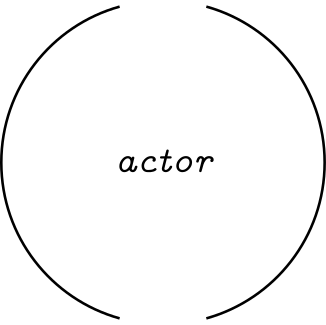
\includegraphics[width=0.75\linewidth]{chapters/4-MDC_model_application/image/bvl-actor-o.png}
    &
    \centering
    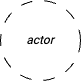
\includegraphics[width=0.75\linewidth]{chapters/4-MDC_model_application/image/bvl-actor.png}
    & 
    The \textit{actor} is represented by a dashed circle with the actor's name in the centre. The circle represents the performer, the audience, the environment, or other external factors interacting with the artwork through ‘gestures’. The actor can be extended with further details. For example, a performer can be represented by two other actor elements representing both hands. Additional information can also be added through text next to the circle. 
    \\\hline
    %%%%%%%%%%%%%%%%%%%%%%%%%%%%%%%%%%%%%%%%%%%%%%%%%%%%%%%%%%%%%%%%%%%%%%%%%%%%%%%%%%%%%%%%%%%%%%%%%%%%
    %%%%%%%%%%%%%%%%%%%%%%%%%%%%%%%%%%%%%%%%%%%%%%%%%%%%%%%%%%%%%%%%%%%%%%%%%%%%%%%%%%%%%%%%%%%%%%%%%%%%
    \centering
    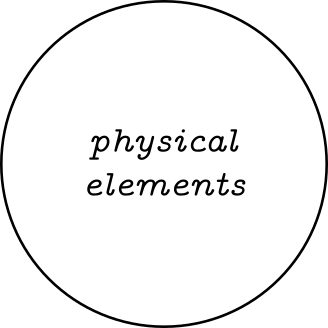
\includegraphics[width=0.75\linewidth]{chapters/4-MDC_model_application/image/bvl-physicalelement-o.png}
    &
    \centering
    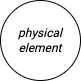
\includegraphics[width=0.75\linewidth]{chapters/4-MDC_model_application/image/bvl-physicalelement.png}
    & 
    The \textit{physical} element is represented by a solid circle with the element's name in the centre. It represents the physical \textit{bit} (e.g., hardware) with which the actor interacts. Text next to the circle can also provide further information.
    \\\hline
    %%%%%%%%%%%%%%%%%%%%%%%%%%%%%%%%%%%%%%%%%%%%%%%%%%%%%%%%%%%%%%%%%%%%%%%%%%%%%%%%%%%%%%%%%%%%%%%%%%%%
    %%%%%%%%%%%%%%%%%%%%%%%%%%%%%%%%%%%%%%%%%%%%%%%%%%%%%%%%%%%%%%%%%%%%%%%%%%%%%%%%%%%%%%%%%%%%%%%%%%%%
    \centering
    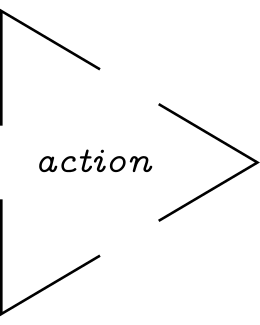
\includegraphics[width=0.75\linewidth]{chapters/4-MDC_model_application/image/bvl-action-o.png}
    &
    \centering
    
\includegraphics[width=0.75\linewidth]{chapters/4-MDC_model_application/image/bvl-action.png}
    & 
    The \textit{action} is represented by a dashed triangle pointing to the right and with the name of the specific action in the centre. The element represents the action (or gesture) produced by the actor. It can be used with the actor (``press'' a button) or with the physical element (e.g. the bow ``move'' in the cello’s string). Further information can also be added through text next to the circle.
    \\\hline
    %%%%%%%%%%%%%%%%%%%%%%%%%%%%%%%%%%%%%%%%%%%%%%%%%%%%%%%%%%%%%%%%%%%%%%%%%%%%%%%%%%%%%%%%%%%%%%%%%%%%
    %%%%%%%%%%%%%%%%%%%%%%%%%%%%%%%%%%%%%%%%%%%%%%%%%%%%%%%%%%%%%%%%%%%%%%%%%%%%%%%%%%%%%%%%%%%%%%%%%%%%
    \centering
    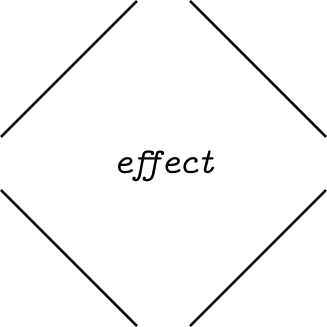
\includegraphics[width=0.75\linewidth]{chapters/4-MDC_model_application/image/bvl-effect-o.png}
    &
    \centering
    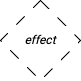
\includegraphics[width=0.75\linewidth]{chapters/4-MDC_model_application/image/bvl-effect.png}
    & 
    The \textit{effect} element is represented by a dashed rhombus with the name (or brief explanation) of the element in the centre. The \textit{effect} should always be at the end of the chain, explaining the effect (the result) produced by the same chain, i.e. by the artwork.
    \\\hline
    %%%%%%%%%%%%%%%%%%%%%%%%%%%%%%%%%%%%%%%%%%%%%%%%%%%%%%%%%%%%%%%%%%%%%%%%%%%%%%%%%%%%%%%%%%%%%%%%%%%%
    %%%%%%%%%%%%%%%%%%%%%%%%%%%%%%%%%%%%%%%%%%%%%%%%%%%%%%%%%%%%%%%%%%%%%%%%%%%%%%%%%%%%%%%%%%%%%%%%%%%%
    \centering
    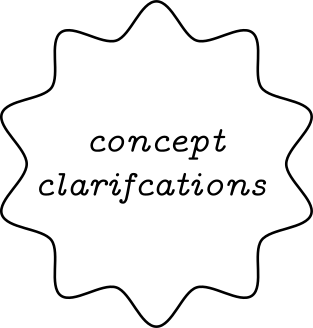
\includegraphics[width=0.75\linewidth]{chapters/4-MDC_model_application/image/bvl-concept-o.png}
    &
    \centering
    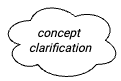
\includegraphics[width=0.75\linewidth]{chapters/4-MDC_model_application/image/bvl-concept.png}
    & 
    The \textit{concept clarification} element is represented by a solid cloud with a short text explaining the concept in the centre. This element enhances the information about the described concept and is usually placed near the \textit{action} or \textit{effect} elements. While the other elements are linked between them, this element is used without a link and placed near the element (or group of elements) that necessitates an in-depth explanation
    \\\hline
    %%%%%%%%%%%%%%%%%%%%%%%%%%%%%%%%%%%%%%%%%%%%%%%%%%%%%%%%%%%%%%%%%%%%%%%%%%%%%%%%%%%%%%%%%%%%%%%%%%%%
\end{longtable}

Except for the \textit{concept clarification} element, all other elements are connected by directional arrows to show the flow of actions and elements. In our implementation, we also include text above or below the links to provide more details about the relationships (e.g., the \textit{Conceptual Mapping} of Michele Sambin’s video loop in Figure~\ref{}). Finally, as mentioned earlier, the \textit{effect} element represents the output of the flowchart.\\
In Figure~\ref{fig:c4-conceptual_level} below, we present an example of a \textit{Conceptual Mapping} flow diagram created by Baalman in her book, recreated using our implementation.
\begin{figure}[!h]
    \centering
    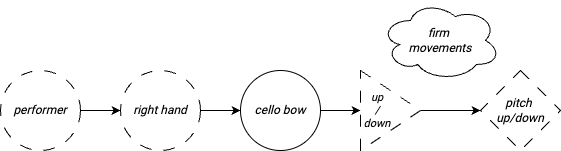
\includegraphics[width=1\linewidth]{chapters/4-MDC_model_application/image/bvl-conceptual_level.png}
    \caption{BVL application for \textit{Conceptual Mapping}. The mapping is proposed in \cite{baalman2022composing}.}
    \label{fig:c4-conceptual_level}
\end{figure}
This diagram illustrates a simple interaction where a performer can change the pitch of a cello by moving the bow (held in their right hand) vertically with firm movements, either upward or downward.\\
In this text, we have examined several conceptual mappings, starting with the introduction of the BVL in Chapter~\ref{ch:3-mdc_model-reactivation_workflow-instruction_template} (Figure~\ref{fig:c3-BVLconceptual}) and throughout the appendices (Appendix~\ref{ax:a-michele_sambin_videoloop}, Figure~\ref{}; Appendix~\ref{ax:b-hybrid_reactivation_il_caos_delle_sfere}, Figure~\ref{}; and Appendix~\ref{ax:d-sustainability_and_longevity_of_nimes}, Figure~\ref{}). All these \textit{Conceptual Mappings} describe different scenarios, yet they can be easily explained using these essential elements.

\subsection{Physical implementation Level}
The \textit{Physical Implementation Mapping} describes what happens between the gesture and the output, focusing specifically on the ``physical'' level, including various interfaces, hardware, and software. In this context, we need to define four main elements, three types of connections, and six types of streams. Table~\ref{tab:c4-bvl_physical} define the adaptation of the four main elements.

\begin{longtable}{|m{0.18\textwidth}|m{0.18\textwidth}|m{0.55\textwidth}|}
    \caption{Adaptation of BVL boxes to \textit{Physical Implementation Level}} \label{tab:c4-bvl_physical} \\
    \hline
    \textbf{Original} & \textbf{Adapted} & \textbf{Description} \\
    \hline
    %%%%%%%%%%%%%%%%%%%%%%%%%%%%%%%%%%%%%%%%%%%%%%%%%%%%%%%%%%%%%%%%%%%%%%%%%%%%%%%%%%%%%%%%%%%%%%%%%%%%
    \centering
    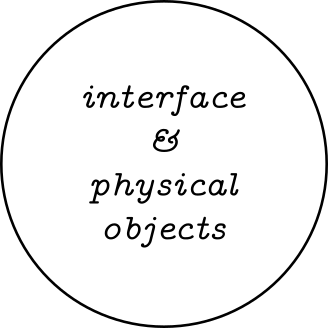
\includegraphics[width=0.75\linewidth]{chapters/4-MDC_model_application/image/bvl-interface-o.png}
    &
    \centering
    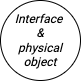
\includegraphics[width=0.75\linewidth]{chapters/4-MDC_model_application/image/bvl-interface.png}
    & 
    The \textit{interface \& physical object} is represented by a solid circle with the element's name in the centre. This element represents the physical element with which the interaction occurs. Further information can also be added through text next to the circle.
    \\\hline
    %%%%%%%%%%%%%%%%%%%%%%%%%%%%%%%%%%%%%%%%%%%%%%%%%%%%%%%%%%%%%%%%%%%%%%%%%%%%%%%%%%%%%%%%%%%%%%%%%%%%
    %%%%%%%%%%%%%%%%%%%%%%%%%%%%%%%%%%%%%%%%%%%%%%%%%%%%%%%%%%%%%%%%%%%%%%%%%%%%%%%%%%%%%%%%%%%%%%%%%%%%
    \centering
    \includegraphics[width=0.75\linewidth]{chapters/4-MDC_model_application/image/bvl-hardware-o.png}
    &
    \centering
    \includegraphics[width=0.75\linewidth]{chapters/4-MDC_model_application/image/bvl-hardware.png}
    & 
    The \textit{hardware} is represented by a solid square with the name of the specific hardware in the centre. This element represents any kind of hardware. Further information can also be added through text next to the square.
    \\\hline
    %%%%%%%%%%%%%%%%%%%%%%%%%%%%%%%%%%%%%%%%%%%%%%%%%%%%%%%%%%%%%%%%%%%%%%%%%%%%%%%%%%%%%%%%%%%%%%%%%%%%
    %%%%%%%%%%%%%%%%%%%%%%%%%%%%%%%%%%%%%%%%%%%%%%%%%%%%%%%%%%%%%%%%%%%%%%%%%%%%%%%%%%%%%%%%%%%%%%%%%%%%
    \centering
    \includegraphics[width=0.75\linewidth]{chapters/4-MDC_model_application/image/bvl-software-o.png}
    &
    \centering
    \includegraphics[width=0.75\linewidth]{chapters/4-MDC_model_application/image/bvl-software.png}
    & 
    The \textit{software} is represented by a dashed square with the name of the specific software in the centre. This element represents any kind of software. Further information can also be added through text next to the square.
    \\\hline
    %%%%%%%%%%%%%%%%%%%%%%%%%%%%%%%%%%%%%%%%%%%%%%%%%%%%%%%%%%%%%%%%%%%%%%%%%%%%%%%%%%%%%%%%%%%%%%%%%%%%
    %%%%%%%%%%%%%%%%%%%%%%%%%%%%%%%%%%%%%%%%%%%%%%%%%%%%%%%%%%%%%%%%%%%%%%%%%%%%%%%%%%%%%%%%%%%%%%%%%%%%
    \centering
    \includegraphics[width=0.75\linewidth]{chapters/4-MDC_model_application/image/bvl-output-o.png}
    &
    \centering
    \includegraphics[width=0.75\linewidth]{chapters/4-MDC_model_application/image/bvl-output.png}
    & 
    The \textit{output} is represented by a solid triangle pointing to the left, with the name of the specific output in the centre. This element represents the system's output. It should be used at the end of the entire \textit{Physical Implementation Mapping}. Text next to the triangle can also provide further information.
    \\\hline
    %%%%%%%%%%%%%%%%%%%%%%%%%%%%%%%%%%%%%%%%%%%%%%%%%%%%%%%%%%%%%%%%%%%%%%%%%%%%%%%%%%%%%%%%%%%%%%%%%%%%
\end{longtable}

These elements are connected in order to define the flow of the physical implementation. Unlike conceptual mapping, this level involves different types of communication, represented by three types of connections that can be either unidirectional or multidirectional. The connections are:

\begin{longtable}{|m{0.1\textwidth}|m{0.49\textwidth}|m{0.32\textwidth}|}
    \caption{Adaptation of BVL connection arrow for the \textit{Physical Implementation Level}} \label{tab:c4-bvl_physical_arrow} \\
    \hline
    \textbf{} & \textbf{Type of connection} & \textbf{Description} \\
    \hline
    %%%%%%%%%%%%%%%%%%%%%%%%%%%%%%%%%%%%%%%%%%%%%%%%%%%%%%%%%%%%%%%%%%%%%%%%%%%%%%%%%%%%%%%%%%%%%%%%%%%%
    %%%%%%%%%%%%%%%%%%%%%%%%%%%%%%%%%%%%%%%%%%%%%%%%%%%%%%%%%%%%%%%%%%%%%%%%%%%%%%%%%%%%%%%%%%%%%%%%%%%%
    \centering
    \small \textbf{Original} \rule{0pt}{1.25cm} & 
    \centering
    \includegraphics[width=1\linewidth]{chapters/4-MDC_model_application/image/bvl-arrow-wired-o.png} &
    \multirow{2}{*}{\parbox[t]{\linewidth}{\vspace{-1cm}The \textit{wired} connection is represented by a directional solid line. The type of connection used for the link replaces the ``protocol'' word (e.g. Audio, USB, etc.).}}
    \\
    \centering
    \small \textbf{Adapted} \rule{0pt}{1.25cm} &
    \centering
    \includegraphics[width=1\linewidth]{chapters/4-MDC_model_application/image/bvl-arrow-wired.png} & 
    \\
    \hline
    %%%%%%%%%%%%%%%%%%%%%%%%%%%%%%%%%%%%%%%%%%%%%%%%%%%%%%%%%%%%%%%%%%%%%%%%%%%%%%%%%%%%%%%%%%%%%%%%%%%%
    %%%%%%%%%%%%%%%%%%%%%%%%%%%%%%%%%%%%%%%%%%%%%%%%%%%%%%%%%%%%%%%%%%%%%%%%%%%%%%%%%%%%%%%%%%%%%%%%%%%%
    \centering
    \small \textbf{Original} \rule{0pt}{1.43cm} & 
    \centering
    \includegraphics[width=1\linewidth]{chapters/4-MDC_model_application/image/bvl-arrow-wireless-o.png} &
    \multirow{2}{*}{\parbox[t]{\linewidth}{\vspace{-1.05cm}The \textit{wireless} connection is represented by a directional dotted line (originally by a dash-dotted line). The protocol type replaces the ``protocol'' word (e.g. Wi-Fi, Bluetooth, etc.).}}
    \\
    \centering
    \small \textbf{Adapted} \rule{0pt}{1.43cm} &
    \centering
    \includegraphics[width=1\linewidth]{chapters/4-MDC_model_application/image/bvl-arrow-wireless.png} & 
    \\
    \hline
    %%%%%%%%%%%%%%%%%%%%%%%%%%%%%%%%%%%%%%%%%%%%%%%%%%%%%%%%%%%%%%%%%%%%%%%%%%%%%%%%%%%%%%%%%%%%%%%%%%%%
    %%%%%%%%%%%%%%%%%%%%%%%%%%%%%%%%%%%%%%%%%%%%%%%%%%%%%%%%%%%%%%%%%%%%%%%%%%%%%%%%%%%%%%%%%%%%%%%%%%%%
    \centering
    \small \textbf{Original} \rule{0pt}{1.25cm} & 
    \centering
    \includegraphics[width=1\linewidth]{chapters/4-MDC_model_application/image/bvl-arrow-software-o.png} &
    \multirow{2}{*}{\parbox[t]{\linewidth}{\vspace{-1cm}The \textit{software} connection is represented with a directional dashed line. It is usually used between hardware and software to indicate which hardware runs a specific software.}}
    \\
    \centering
    \small \textbf{Adapted} \rule{0pt}{1.25cm} &
    \centering
    \includegraphics[width=1\linewidth]{chapters/4-MDC_model_application/image/bvl-arrow-software.png} & 
    \\
    \hline
    %%%%%%%%%%%%%%%%%%%%%%%%%%%%%%%%%%%%%%%%%%%%%%%%%%%%%%%%%%%%%%%%%%%%%%%%%%%%%%%%%%%%%%%%%%%%%%%%%%%%
\end{longtable}

Furthermore, this connection can have six different types of streams. The types are adapted with just a series of characters and should be placed above the connection at the beginning. The types of streams are shown in Table~\ref{tab:c4-bvl_physical_strem}

\begin{longtable}{|m{0.05\textwidth}|m{0.05\textwidth}|m{0.81\textwidth}|}
    \caption{Adaptation of BVL streams for \textit{Physical Implementation Level}} \label{tab:c4-bvl_physical_strem} \\
    \hline
    \textbf{Ori.} & \textbf{Ada.} & \textbf{Description} \\
    \hline
    %%%%%%%%%%%%%%%%%%%%%%%%%%%%%%%%%%%%%%%%%%%%%%%%%%%%%%%%%%%%%%%%%%%%%%%%%%%%%%%%%%%%%%%%%%%%%%%%%%%%
    \centering
    \includegraphics[width=0.75\linewidth]{chapters/4-MDC_model_application/image/bvl-audio-o.png}
    &
    \centering
    \includegraphics[width=0.75\linewidth]{chapters/4-MDC_model_application/image/bvl-audio.png}
    & 
    The \textit{Audio} stream is represented by the tilde character ($\sim$).
    \\\hline
    %%%%%%%%%%%%%%%%%%%%%%%%%%%%%%%%%%%%%%%%%%%%%%%%%%%%%%%%%%%%%%%%%%%%%%%%%%%%%%%%%%%%%%%%%%%%%%%%%%%%
    %%%%%%%%%%%%%%%%%%%%%%%%%%%%%%%%%%%%%%%%%%%%%%%%%%%%%%%%%%%%%%%%%%%%%%%%%%%%%%%%%%%%%%%%%%%%%%%%%%%%
    \centering
    \includegraphics[width=0.75\linewidth]{chapters/4-MDC_model_application/image/bvl-video-o.png}
    &
    \centering
    \includegraphics[width=0.75\linewidth]{chapters/4-MDC_model_application/image/bvl-video.png}
    & 
    The \textit{video} stream is represented by the open and closed square bracket with a space in between ([ ]). 
    \\\hline
    %%%%%%%%%%%%%%%%%%%%%%%%%%%%%%%%%%%%%%%%%%%%%%%%%%%%%%%%%%%%%%%%%%%%%%%%%%%%%%%%%%%%%%%%%%%%%%%%%%%%
    %%%%%%%%%%%%%%%%%%%%%%%%%%%%%%%%%%%%%%%%%%%%%%%%%%%%%%%%%%%%%%%%%%%%%%%%%%%%%%%%%%%%%%%%%%%%%%%%%%%%
    \centering
    \includegraphics[width=0.75\linewidth]{chapters/4-MDC_model_application/image/bvl-data-o.png}
    &
    \centering
    \includegraphics[width=0.75\linewidth]{chapters/4-MDC_model_application/image/bvl-data.png}
    & 
    The \textit{data} stream is represented by the pipe characters (\textbar) and the capital o (\textbar O).
    \\\hline
    %%%%%%%%%%%%%%%%%%%%%%%%%%%%%%%%%%%%%%%%%%%%%%%%%%%%%%%%%%%%%%%%%%%%%%%%%%%%%%%%%%%%%%%%%%%%%%%%%%%%
    %%%%%%%%%%%%%%%%%%%%%%%%%%%%%%%%%%%%%%%%%%%%%%%%%%%%%%%%%%%%%%%%%%%%%%%%%%%%%%%%%%%%%%%%%%%%%%%%%%%%
    \centering
    \includegraphics[width=0.75\linewidth]{chapters/4-MDC_model_application/image/bvl-event-o.png}
    &
    \centering
    \includegraphics[width=0.75\linewidth]{chapters/4-MDC_model_application/image/bvl-event.png}
    & 
    The \textit{event} stream is represented by the capital slashed o character (\O).
    \\\hline
    %%%%%%%%%%%%%%%%%%%%%%%%%%%%%%%%%%%%%%%%%%%%%%%%%%%%%%%%%%%%%%%%%%%%%%%%%%%%%%%%%%%%%%%%%%%%%%%%%%%%
    %%%%%%%%%%%%%%%%%%%%%%%%%%%%%%%%%%%%%%%%%%%%%%%%%%%%%%%%%%%%%%%%%%%%%%%%%%%%%%%%%%%%%%%%%%%%%%%%%%%%
    \centering
    \includegraphics[width=0.75\linewidth]{chapters/4-MDC_model_application/image/bvl-buffer-o.png}
    &
    \centering
    \includegraphics[width=0.75\linewidth]{chapters/4-MDC_model_application/image/bvl-buffer.png}
    & 
    The buffer stream is represented by four pipe characters (\textbar\textbar\textbar\textbar).
    \\\hline
    %%%%%%%%%%%%%%%%%%%%%%%%%%%%%%%%%%%%%%%%%%%%%%%%%%%%%%%%%%%%%%%%%%%%%%%%%%%%%%%%%%%%%%%%%%%%%%%%%%%%
    %%%%%%%%%%%%%%%%%%%%%%%%%%%%%%%%%%%%%%%%%%%%%%%%%%%%%%%%%%%%%%%%%%%%%%%%%%%%%%%%%%%%%%%%%%%%%%%%%%%%
    \centering
    \includegraphics[width=0.75\linewidth]{chapters/4-MDC_model_application/image/bvl-spectral-o.png}
    &
    \centering
    \includegraphics[width=0.75\linewidth]{chapters/4-MDC_model_application/image/bvl-spectral.png}
    & 
    The spectral stream is represented by the lozenge (or Diamond) character ($\lozenge$).
    \\\hline
    %%%%%%%%%%%%%%%%%%%%%%%%%%%%%%%%%%%%%%%%%%%%%%%%%%%%%%%%%%%%%%%%%%%%%%%%%%%%%%%%%%%%%%%%%%%%%%%%%%%%
\end{longtable}
We can include text for each element and connection to provide additional details or explanations.
Figure~\ref{fig:c4-physical_level} presents a straightforward example of a \textit{Physical Implementation Mapping} diagram using our implementation of the BVL created with Diagram.net. This example shows a basic setup in which a sound card is connected to a computer running Max/MSP, a microphone (the interaction \textit{interface}), and a speaker (the \textit{output}).\\
For elements like \textit{Interface \& Physical Object}, and \textit{Hardware}, we can add more detailed information, such as the type and name of the input or output devices. In Figure~\ref{fig:c4-physical_level02}, we see two examples: the Adafruit BNO085, a motion sensor with an integrated accelerometer, gyroscope, and magnetometer, and an audio mixer with various types of audio inputs and outputs.\\
\begin{minipage}[t]{0.45\textwidth}
    \centering
    \includegraphics[width=\linewidth]{chapters/4-MDC_model_application/image/bvl-physical_level.png}
    \captionof{figure}{Simple BVL application for \textit{Physical Implementation Mapping}.}
    \label{fig:c4-physical_level}
\end{minipage}%
\hfill
\begin{minipage}[t]{0.45\textwidth}
    \centering
    \includegraphics[width=\linewidth]{chapters/4-MDC_model_application/image/bvl-physical_level02.png}
    \captionof{figure}{\textit{Interface \& Physical Object} (above), and \textit{Hardware} (below) examples with input and output details.}
    \label{fig:c4-physical_level02}
\end{minipage}
\newline
In this text, we have examined many \textit{Physical Implementation Mappings}, starting with the introduction of the BVL in Chapter~\ref{ch:3-mdc_model-reactivation_workflow-instruction_template} (Figure~\ref{fig:c3-BVLphysical}) and throughout the appendices (Appendix~\ref{ax:a-michele_sambin_videoloop}, Figure~\ref{}; Appendix~\ref{ax:b-hybrid_reactivation_il_caos_delle_sfere}, Figures~\ref{}, \ref{}, and \ref{}; and Appendix~\ref{ax:d-sustainability_and_longevity_of_nimes}, Figure~\ref{}).

\subsection{Process Level}
\textit{Process Mapping} involves a potentially infinite set of blocks that can be organised to describe, at a computational level, what happens between a gesture and the output—how one type of data is transformed into another. This description can be provided at different levels of detail, corresponding to various types of operations, ranging from low-level tasks (e.g., addition or subtraction) to higher-level processes (e.g., resampling).\\
The level of detail required depends on several factors, such as the complexity of the work, the need for detail (e.g., it may not be necessary to describe a low-pass filter in full detail), and practical considerations like the time, resources, and personnel available. Striking the right balance between description complexity and feasibility is not always straightforward, and in many cases, achieving a highly detailed level of description may not be possible.\\
The BVL defines a limited set of blocks, which are insufficient based on our applications. To address this, we propose an extended system within the context of our implementation. This system includes two block types: the \textit{Operation} and \textit{Function} blocks, which can be adapted to specific operations and processes.
While the \textit{Operation} block simply describes a defined operation, the \textit{Function} block describes a new process through a series of operations. The \textit{Function} block encapsulates another process that can be described using a separate \textit{Process Mapping}. This nested system can contain additional \textit{Function} blocks, creating a matryoshka-like structure. This approach helps simplify individual mappings, which might otherwise become overly complex and difficult to read.

\begin{longtable}{|m{0.30\textwidth}|m{0.68\textwidth}|}
    \caption{Adaptation of BVL blocks to the \textit{Process Level}} \label{tab:c4-bvl_process} \\
    \hline
    \textbf{Block} & \textbf{Description} \\
    \hline
    %%%%%%%%%%%%%%%%%%%%%%%%%%%%%%%%%%%%%%%%%%%%%%%%%%%%%%%%%%%%%%%%%%%%%%%%%%%%%%%%%%%%%%%%%%%%%%%%%%%%
    \centering
    \includegraphics[width=0.5\linewidth]{chapters/4-MDC_model_application/image/bvl-operation.png}
    & 
    The \textit{Operation Block} (\textit{Op. Block}) allow us to define a custom operation in the process mapping. It is represented by a square with the symbol of the operation in the centre (\$), which has to be replaced with the custom operation symbol. In the left-bottom corner, we have the extended name of the operation (\textit{Op. Block}), abbreviated if it is too long. On the left side, we have a series of defined inputs (\textit{inN}) and on the right side, a series of defined outputs (\textit{outN}), while at the top, we can have a series of arrows that define \textit{external factors}. We have a short description of the custom operation block below the box.
    \\\hline
    %%%%%%%%%%%%%%%%%%%%%%%%%%%%%%%%%%%%%%%%%%%%%%%%%%%%%%%%%%%%%%%%%%%%%%%%%%%%%%%%%%%%%%%%%%%%%%%%%%%%
    %%%%%%%%%%%%%%%%%%%%%%%%%%%%%%%%%%%%%%%%%%%%%%%%%%%%%%%%%%%%%%%%%%%%%%%%%%%%%%%%%%%%%%%%%%%%%%%%%%%%
    \centering
    \includegraphics[width=0.75\linewidth]{chapters/4-MDC_model_application/image/bvl-function.png}
    & 
    The \textit{Function block} (\textit{Function}) allows us to create custom functions. Functions are abstractions of a part of the \textit{Process Mapping} and help keep the process clear and readable. A function is represented by a rectangular shape with the function's name at the centre, a series of defined inputs and outputs on the sides, a series of defined initialisation arguments, and a short description below the shape.
    \\\hline
    %%%%%%%%%%%%%%%%%%%%%%%%%%%%%%%%%%%%%%%%%%%%%%%%%%%%%%%%%%%%%%%%%%%%%%%%%%%%%%%%%%%%%%%%%%%%%%%%%%%%
\end{longtable}
With the \textit{Operation} block, we can create custom operations, such as those presented in the Baalmans’ book \cite{baalman2022composing} (Figure~\ref{fig:c4-process_level}).
\begin{figure}[!h]
    \centering
    \includegraphics[width=1\linewidth]{chapters/4-MDC_model_application/image/bvl-process_level.png}
    \caption{Example of \textit{Operation} Block, constructed using the method above. Some of them are extracted from \cite{baalman2022composing}.}
    \label{fig:c4-process_level}
\end{figure}
The different components used to describe an \textit{Operation} block are always optional. For example, the \textit{Range} block does not include a symbol. In other cases, the symbol can be expanded—such as in the \textit{Gate} block—to represent the block's functionality better.\\
The \textit{Function} block allows us to simplify the mapping of a specific process, making it easier to read and understand. For example, consider the mapping in Figure~\ref{fig:c4-process_mapping02}.
\begin{figure}[!h]
    \centering
    \includegraphics[width=0.7\linewidth]{chapters/4-MDC_model_application/image/bvl-process_level02.png}
    \caption{An example of Process mapping using a \textit{Function} block. To simplify the mapping. Figure~\ref{fig:c4-process_level03} represent the process inscribed inside the Function block \textit{Simple Pedometer}.}
    \label{fig:c4-process_level02}
\end{figure}
In this straightforward example, the mapping is easy to read. It illustrates that light is switched on for each step detected by a pedometer (which uses the three axes of an accelerometer as input). The \textit{Function} Block \textit{Simple Pedometer} serves as an abstraction, encapsulating a more detailed process mapping. This abstraction simplifies the main mapping, making it easier to read. The \textit{Simple Pedometer} can be expanded into the detailed mapping in Figure~\ref{fig:c4-process_level03}. This mapping represents the pedometer process, which, if included in the mapping from the previous figure, would have made the entire process significantly more complex to read.
\begin{figure}[!h]
    \centering
    \includegraphics[width=\linewidth]{chapters/4-MDC_model_application/image/bvl-process_level03.png}
    \caption{The \textit{Process mapping} of a pedometer. This process was inscribed inside the \textit{Function} block \textit{Simple Pedometer} in Figure~\ref{fig:c4-process_level02}.}
    \label{fig:c4-process_level03}
\end{figure}
Furthermore, the last mapping in Fgure~\ref{fig:c4-process_level03} presents a new type of block (Figure~\ref{fig:c4-bvl-buffer}). 
\begin{figure}[!h]
    \centering
    \includegraphics[width=0.2\linewidth]{chapters/4-MDC_model_application/image/bvl-bufferblock.png}
    \caption{The \textit{Process Mapping}'s \textit{Buffer} block.}
    \label{fig:c4-bvl-buffer}
\end{figure}
This block type can describe a sequence of numbers or bits, such as arrays or buffers. In previous mappings (Figures~\ref{fig:c4-process_level02} and \ref{fig:c4-process_level03}), we also see the \textit{Interface & Physical Objects} block, which can be used to define input data more precisely. Similarly, the Output block can specify the output type in greater detail.
In process mapping, we can generally incorporate all other types of objects defined at higher levels to better clarify and contextualise the process.\\
In this text, we have examined many \textit{Process Mappings}, starting with the introduction of the BVL in Chapter~\ref{ch:3-mdc_model-reactivation_workflow-instruction_template} (Figure~\ref{fig:c3-BVLprocess}) and throughout the appendices (Appendix~\ref{ax:a-michele_sambin_videoloop}, Figure~\ref{}; Appendix~\ref{ax:b-hybrid_reactivation_il_caos_delle_sfere}, Figures~\ref{}; and Appendix~\ref{ax:d-sustainability_and_longevity_of_nimes}, Figure~\ref{}).

\section{Summary}
In this chapter, we demonstrated how to apply the MDC model on three different platforms: 1) using the Neo4j graph database, 2) using the GitHub development platform, and 3) using Apple’s Finder file management system. These applications highlight the model’s adaptability to various use cases and levels of complexity: 1) a more extensive, comprehensive application that could reflect the needs of a web-based or private archive for an organisation (e.g., a museum), 2) a more collaborative approach where conservation happens alongside the development of creative work, 3) a simpler, more individual application that can be used in a preliminary phase (e.g., the collection phase) of a reactivation or to organise a personal archive (an “actor’s archive”), especially when copyright restrictions are involved. Although we see that, from the first application to the last, the MDC model becomes increasingly abstract—removing details and simplifying basic properties (such as \textit{multiple belongingness})—we also notice that they all share the same language. For example, in these three applications, it’s easy to move from an “actor’s archive” to a GitHub repository, or from GitHub to a Neo4j database, and back again. In all three cases, we always have an archive containing all the components, instructions, and technical information, as well as images and videos. Whether it’s in an “archive” folder, in the main directory (as with Patricia Cadavid’s instruments), or in another structure, each element is independently functional, has its own descriptive record (according to our metadata schema), and, if digital (code, audio, video, etc.), is often found within the archive itself. We also have folders, text files, or nodes representing the set of iterations that allow us to reconstruct the substance of the various archived elements. According to the MDC model, each element belongs to the artwork based on its function within a particular iteration. Hence, inside each iteration, we have links—whether they are relationships between nodes, hypertext links, or aliases—through which we can identify the roles and qualities of each component in relation to the creative work’s life cycle or biography.\\
This model aims to promote adaptability and flexibility in its application while also fostering the shareability and collaboration of the various entities involved in creating and conserving creative work.\\
The same principle of adaptability and flexibility applies to the BVL introduced at the end of this chapter. In this case, we adapted and slightly extended the language in the context of Diagram.net, but as the original author suggests, the language can also be used on paper. The language offers a straightforward description method, and—especially in our adaptation—the main elements to consider are: 3 levels of description (conceptual, physical, process), 12 boxes (two of which, “Operation” and “Function,” can be significantly expanded), 3 connection types, and 6 signal flow types. Using just these elements, along with written explanations, we can describe any kind of creative work and any process involved, going into more or less detail as we choose.


    % conclusion ---------------
    %!TEX root = ../main.tex

\chapter*{\label{ch:conclusions}Conclusions}
\markboth{Conclusions}{}
\addcontentsline{toc}{chapter}{Conclusions} 
% NOTE: Introduction and Conclusions are special chapters: they are not
%       marked by a section number, so we need to add it manually to the
%       ToC, as done above.

The main research question posed at the beginning of this thesis was: \textit{How can live media art be kept alive?} This question underpins the conceptual framework developed throughout the research and serves as the foundation for its main contributions: the model for documenting, reactivating, and conserving contemporary artistic practices.\\
As discussed in Chapters~\ref{ch:1-state_of_the_art} and~\ref{ch:2-new_conservation_paradigms}, conservation has shifted from preserving an artwork's ``original'', ``authentic'' state to safeguarding the conditions that allow the artwork to unfold. Conservation now involves keeping the artwork ``alive'' through its various reactivations, allowing it to form and reform within the ever-changing dynamics of its experiential ecosystem. Artworks are no longer static objects bound to an absolute idea of experience but are instead defined by those experiences generated within specific socio-cultural contexts, making them as ephemeral as those contexts. Contemporary artistic practices often utilise media and technology to explore the expressive possibilities of these tools, detaching them from their practical functions. Such practices highlight the convergence of aesthetic and social functions within a single expression, reflecting on how humans live within, think about, and interact with their technological ecosystems.\\
Case studies and examples in the text demonstrate how contemporary art inquiries the expressive potential of technology within socio-cultural and experiential contexts. For instance, Michele Sambin’s \textit{videoloop} (Appendix~\ref{ax:a-michele_sambin_videoloop}) demonstrates how real-time video technology can transform linear time into circular time, turning a monologue into a dialogue between potentially infinite entities. The work starts with the intrinsic capabilities of the video device and expands into heightened experiences of its everyday functionality. The familiar LCD (or CRT) screen, commonly used daily for work, meetings, movies, and news, is reimagined on stage to distort time and create a self-dialogue. This transformation highlights how the same screen, with unchanged affordances, can evoke entirely new meanings, highlighting the hidden expressive and interactive potentials of ubiquitous technologies. Similarly, \textit{Il caos delle sfere} (Appendix~\ref{ax:b-hybrid_reactivation_il_caos_delle_sfere}) and \textit{The Hole in Space} employ ``current'' and popular technologies to create innovative experiential contexts. These works merge aesthetic and social functions, inviting audiences to rethink familiar devices and their cultural implications. Another example is Patricia Cadavid’s instruments (Appendix~\ref{ax:d-sustainability_and_longevity_of_nimes}), which emerge from the intersection of two ecosystems: traditional Colombian cultural heritage and the experimental context of New Interfaces for Musical Expression (NIME). These instruments depend on both ecosystems and evolve through interaction, blending cultural affordances with expressive potential in a contemporary framework.\\
These examples underline a critical point: artworks cannot be separated from their aesthetic or social functions. Conservation must account for the ecosystems in which the artwork operates, ensuring its capacity to evolve alongside socio-cultural transformations. This approach allows the artwork's aesthetic and social functions to survive and grow.\\
For this reason, the artwork's identity cannot remain static and detached from conservation practices, whether carried out by conservators, artists, or both. The artwork must be continuously rebuilt and reinterpreted—not only in its components but in its functionality. The \textit{ecological turn} in conservation practices, as discussed in Chapter~\ref{ch:2-new_conservation_paradigms}, emphasises the idea of the artwork as a living organism with its own \textit{biography}. Its life unfolds through the negotiation of interactions among various ecosystems—technological, institutional, creative, and, in general, socio-cultural—during reactivations.\\
Documentation is the main instrument used to support conservation and, thus, the artwork unfolding. As seen in Chapter~\ref{ch:2-new_conservation_paradigms}, documentation allows us to trace an artwork’s \textit{biography}, negotiate interactions between ecosystems, and understand its \textit{variability} and \textit{changeability}. It describes technologies, devices, and elements within the artwork, their origins, and their roles. It captures the artist’s vision, collaborators’ contributions, and the forming identity of the work across iterations. Documentation also forms the foundation for innovative conservation methodologies, as explored in Chapter~\ref{ch:1-state_of_the_art}. Over the past three decades, international initiatives have developed tools such as interviews, questionnaires, instruction modules, thesauri, and identity-definition frameworks. Among these, tracing the identity and iterations of an artwork through structured documentation templates has emerged as a critical, innovative aspect. However, despite progress in this research field, a fully standardised approach, with its benefits, remains elusive, and it may never be possible. Conservation practices and artworks remain deeply tied to the institutions and ecosystems in which they are embedded.\\
Based on this awareness, the primary contribution of this research is the \textit{Multilevel Dynamic Conservation} (MDC) model. The goal is not to pursue standardisation but to promote the heterogeneity of conservation applications, emphasising flexibility and adaptability. The model functions as a meta-model, where the prefix ``meta'' denotes an abstraction of conservation paradigms and models for live media art. Its purpose is to define the hierarchical, multilevel properties of live media art’s creative works within the context of their conservation, including the \textit{multiple belongingness} (connections between and within iterations) and the \textit{dependencies} of various levels of the work. \\
This framework aims to establish guidelines for both applying and describing the conservation of live media art. It provides a versatile tool for a wide range of entities involved in the creation and preservation of this art form—from the development of tools and technologies to the creation of performance environments and the archiving of works in museums and other institutions. The MDC model offers a methodology to create exclusive, context-specific models, fostering collaboration across diverse applications, tools, and expertise. It emphasises common elements for interaction and exchange across sectors and ecosystems, thereby advancing the \textit{ecological turn} at the archival level –through \textit{dependencies}– and, most importantly, at the practical level.\\
Significantly, to move away from standardisation, this model should not be seen as limited to documentation. While it was applied mainly to archival contexts during this research (as discussed in Chapter~\ref{ch:4-madc_model_application} and demonstrated in the case studies), its scope extends beyond these applications. Drawing from the concept of the \textit{multi-typological} archive in Chapter~\ref{ch:3-mdc_model-reactivation_workflow-instruction_template}, the model avoids categorising elements into exclusive typologies. Instead, it embraces the conservation and archival elements as abstractions–whether they are digital or physical documents, hardware or software components, materials, consumable objects, etc.–focusing on how they interact between them and across the iterations and, thus, how they contribute to the evolving identity of the artwork.\\
It is also essential to note that the variability of the artwork is not an intrinsic property of the model but rather predicted and derived through its application. For instance, the concept of \textit{multiple belongingness} across iterations can also be used to affirm an artwork's immutability. If all elements remain unchanged across iterations, connected by their \textit{multiple belongingness}, the artwork's identity and authenticity can be considered fixed. This traceability of changes can document experiential elements or even track factors of degradation and wear.\\
Therefore, although the model draws on the state-of-the-art (analysis in Chapter~\ref{ch:1-state_of_the_art}) and the conceptual framework of conservation (outlined in Chapter~\ref{ch:2-new_conservation_paradigms}) of live media art, it is not exclusively tied to these contexts. The MDC model promotes openness, flexibility, and adaptability to other perspectives and conceptual frameworks, whether traditional, historical, future-oriented, or merely different.\\
In addition, this research introduces two complementary tools specifically designed for the conservation of live media art: the CATTA reactivation workflow and the \textit{Modular Instruction Framework} (MIF).\\
Grounded in the central role of documentation and the conservation concept as a loop between documentation and reactivation, the CATTA workflow offers a systematic process for live media art's present and future reactivation. The workflow consists of five sequential steps: \textit{Collection}, \textit{Assessment}, \textit{Transcription}, \textit{Transmission}, and \textit{Archiving}, from which its name is derived. This structured sequence, which is hierarchical, based on dependencies, and not rigidly discrete, reflects the interconnected activities involved in reactivating the artwork. Each step has specific goals and outcomes. As defined by the new conservation paradigms, the final step, \textit{Archiving}, closes the loop between documentation and reactivation, enabling subsequent reactivations and ensuring the artwork remains alive.\\
The last contribution, the MIF, has been developed to address the need for comprehensive technical instructions and detailed information to facilitate the reconstruction and survival of artworks. Drawing on the analogy of instructions in live media art with musical scores—commonly discussed in literature—the MIF builds on case studies of live electronic music scores (Appendix~\ref{ax:c-the_score_in_live_electronics_music}) and integrates elements from \textit{Baalman’s Visual Language} (BVL), a system recently developed by Marija Baalman for multimedia performance documentation. The MIF adopts a modular structure, allowing instructions to be created textually or visually using the BVL. These modules aim to produce a layered description of the artwork for reactivation, encompassing components, parameters, and mappings. The mappings include sublevels such as conceptual, physical, and processual (as defined in the BVL), as well as spatial and temporal aspects. This modular design ensures flexibility and adaptability. Conservators, artists, and collaborators can choose the level of detail for technical instructions, as the modules are optional and can be extended to describe low-level processes if needed. Furthermore, the modularity of the MIF allows for the adaptation of individual modules over the course of the artwork’s iterations and transformations.\\
\newline
These tools—the MDC model, the CATTA reactivation workflow, and the MIF—represent the main contributions of this research project, forming an original system for documenting, reactivating, and conserving live media art. Within these models lies the practical answer to the question posed at the beginning of this text. However, we want to address this question and conclude the text using a well-known paradox in this field of research: the \textit{Ship of Theseus} paradox. This paradox raises the metaphysical question of identity for objects whose parts change over time. At its core is the question: if every part of an object is replaced, does it remain the same object? In the Greek myth, as Theseus and the Athenians sailed from Crete, they gradually replaced the wooden parts of their ship as they deteriorated. All the original parts had been substituted by the time they reached Athens. The paradox asks: is the ship that arrived in Athens the same one that departed from Crete? Through the lens of new conservation paradigms, we shift focus from what the ship was at the start or end of its journey to its \textit{function}: carrying the Athenians across the sea from Crete to Athens. The ship’s parts were replaced as needed to conserve the \textit{function}. In the \textit{ecological turn}, the artwork is seen amidst the ``stormy seas'' of technological and socio-cultural transformations, supported and conserved by its ``crew''—artists, conservators, curators, collaborators, and performers—to safeguard its \textit{function}–aesthetic and social functions. Thus, the paradox should not be viewed as a question of an artwork’s identity but as an illustration of how to keep live media art alive. However, in practice, this metaphor is limited. The variables at play—such as the functions of the artwork, the journeys it undertakes, the challenges it faces, and the ``crew'' who maintain it—differ greatly for each piece. Artworks are heterogeneous, made of diverse elements linked to multiple ecosystems. Their creation processes, as well as the entities responsible for their exhibition and conservation, are equally heterogeneous. If conservation has become about safeguarding or ``keeping alive'' the artwork and its functions, the key principles to achieve this in practice are \textit{flexibility} and \textit{adaptability}. These are the key principles at the base of the systems introduced, which are designed and structured to ensure their applicability in several heterogeneous contexts and meet different needs. 













    
    % appendices ---------------
    \begin{appendices}
        \chapter{\label{ax:a-michele_sambin_videoloop}Michele Sambin's \textit{Videoloop}}

The first and the main case study in this PhD research focuses on the reactivation and conservation of a series of analogue video artworks from the 1970s, created using the \textit{videoloop} technique developed by artist Michele Sambin. This case study was especially important for testing and optimising the \textit{Multilevel Dynamic Conservation} (MDC), the CATTA reactivation workflow, and the \textit{Baalman Visual Language} (BVL), as well as their application in the graph database Neo4j. The artworks underwent multiple iterations, with changes and technological updates from their original analogue form.

\section{Objectives}
The main objectives of this case study, in addition to the application, testing and refinement of the systems introduced in Chapter~\ref{ch:3-mdc_model-reactivation_workflow-instruction_template}, are:
\begin{enumerate}
    \item to explore the role of artists in both technology development and conservation processes;
    \item to study oral history: interview with the artist;
    \item to apply the reactivation through analog-to-digital migration;
    \item to create a Neo4j database according to the MDC model–see Chapter~\ref{ch:4-madc_model_application} for more details.
\end{enumerate}

Il ruolo degli artisti nei processi di sviluppo tecnologico
collaborazione con gli artisti nella conservazione
riattivazione per mezzo di migrazione analogico-digitale
inclusione della Oral history: intervista all'artista

\section{Introduction}
Michele Sambin is a versatile Italian artist who has worked with painting, film, video art, music, and theatre since the 1960s. Technology has always been a key part of his work as an artistic tool. One of Sambin's traits is his experimentation with simple, well-known technologies instead of new and advanced ones. He creates original forms of creative expression by pushing these familiar technologies to their limits. Some examples are the innovative use of the real-time audio-video recording in the 1970s, which led to the development of the \textit{videoloop} technique (discussed in detail in this chapter); the use of digital drawing tablets and Photoshop to interact with stages’ proscenium, which led to the \textit{light painting} technique (in Figure~\ref{fig:aa-light_painting} a photo with the visual effect produced with the technique).\\
\begin{figure}[!h]
    \centering
    \includegraphics[width=\linewidth]{chapters/appendix/a/image/figa-lightpainting.jpg}
    \caption{A photo from \textit{Tutto è vivo} (2008), a production by Michele Sambin with TAM, where the artist used the \textit{light painting} technique.}
    \label{fig:aa-light_painting}
\end{figure}
Sambin is generally known for his innovative work in multimedia experimental theatre. He has recently been notably recognised for his audiovisual performances, which form a fundamental part of his artistic production.\\
Sambin’s theatrical works with the Italian company TAM Teatromusica –which he co-founded– are especially notable. He created and co-created over 40 original productions with TAM that combined live performance with experimental music and video. The first production with TAM was \textit{Armoniche} (1980), where four performers interacted with video projections while playing harmonicas, creating a spatial sound experience. It was with TAM that Sambin developed the \textit{light painting} technique, which was featured in productions like \textit{Musica senza musicisti} (2004), \textit{Squarcione} (2004), \textit{Lux} (2006), and especially \textit{Tutto è vivo} (2008).\\ 
Sambin gained widespread recognition only for his theatre work until the early 2000s. However, with renewed interest in Italian video art in the late 1990s, scholars and experts began to rediscover his earlier experimental film and video art pieces from the 1960s and 70s. These include experimental films such as \textit{Anamnesi} (1968), \textit{1 e 2} (1969), \textit{Blu d'acqua} (1972), \textit{Film a strisce} (1976), and others. And performative video artwork, such as \textit{Spartito per violoncello} (1974), \textit{Concerto per clarino e VTR} (1976), \textit{Autoritratto} (1977), and \textit{VTR\&I} (1978). His \textit{videoloop} technique emerged with this last piece and  \textit{Il tempo consuma} (1978), and it was later used in works like \textit{Anche le mani invecchiano} (1979), \textit{Sax} (1980), \textit{Io mi chiamo Michele} (1980), and many others.\\
Today, the \textit{videoloop} technique and Sambin’s video art performances are considered significant works in Italian video art history, as we can read in many sources (a monographic book \cite{lischi2014michele}; many papers about Sambin’s multimedia art \cite{leuzzi2019re, d2021invenzioni, gallo2021intimacy}, among others; a project about Italian video art, \textit{REWINDItalia} \cite{Leuzzi2015-bh}; a monographic exhibition \cite{dimarino2022silvana}; and a Italian video art exhibition \cite{saba2022videoarte}). 

\subsection*{Videoloop technique}
\begin{quote}
    "The videoloop technique was born as a meeting between the desire to work with the video in real-time and, as often happens, an accidental element. It all started with the fact that inside the open-reel tape package (normally used at the time), I found a piece of duct tape used to repair a cut" \cite{fiordelmondo2023toward}.
\end{quote}
The small piece of duct tape sparked a series of inspirations and connections for the artist. It reminded him of his earlier work with audio tape alongside Teresa Rampazzi, Terry Riley's audio loop technique—where two Revox tape recorders were placed five meters apart, connected by a tape—and his early video experiments. All these ideas came together, leading to the creation of the first \textit{videoloop} in 1978.\\
The \textit{videoloop} is a circular system created by two video recorders with a closed ring tape. The closed ring tape is made through the conjunction of tape extremities. The artist explains the technique as follows: 
\begin{quote}
    "The closed ring tape scrolls between two video recorders which are placed at a specific distance to keep the tape under tension. The tape is dragged by the video recorders’ engines and it spins. The first video recorder works as a recorder, while the second works as a player. The camera placed in front of the monitor is attached to the first video recorder, and the second video recorder is attached to the monitor"\footnote{Translation into English by the author.} \cite{lischi2014michele}. 
\end{quote}
Figure~\ref{fig:aa-videoloop_graph01} shows a graphical representation of the system. With this technique, Sambin finds a way to overlap and accumulate video and sound material endlessly. The artist records himself at regular intervals and interacts with the playback material, becoming the interlocutor of his electronic self \cite{balzola2019arti}.
\begin{figure}[!h]
    \centering
    \includegraphics[width=\linewidth]{chapters/appendix/a/image/grapha-videoloop01.png}
    \caption{Graphical representation of the original analogue \textit{videoloop}.}
    \label{fig:aa-videoloop-graph01}
\end{figure}
With this technique, Michele Sambin created many video art performance pieces. One of the first and most relevant one, \textit{Il tempo consuma} (1978), was performed live just once at Fondazione Bevilacqua La Masa in Venice in 1979. It was also exhibited at the \textit{Camere Incantate} exhibition at the Royal Palace in Milan in 1980, but it was not live. As explained by the artist:\\ 
\begin{quote}
    At the end of the seventies, the excitement for new forms of live performance was slightly declining. The same thing happened to pioneering video art, which was considered no longer of interest” \cite{fiordelmondo2023toward}.
\end{quote}
For these reasons, the works with the \textit{videoloop} didn’t obtain significant feedback for many years, and Sambin was considered mainly for his theatrical works. However, as the artist stated in the documentary film \textit{Più della vita} (2019) by Raffella Rivi and in an interview created explicitly in the context of this case study \cite{fiordelmondo2023toward},  the videoloop is one of the most relevant techniques in his artistic production, which has affected all his subsequent work.

\section{Reactivation}
The reactivation process began in May 2021 and went through five different interactions until October 2024. Although it mainly focused on the performance of \textit{Il tempo consuma}, it also comprehends other historical pieces made with the \textit{videoloop} technique and new experimentations. The reactivation was done using the CATTA reactivation workflow and the MDC models (explained in Chapter~\ref{ch:3-mdc_model-reactivation_workflow-instruction_template}). The process of reactivation was conducted by the author alongside the artist. Each choice was made through an interdisciplinary comparison between the aesthetic aspects emphasised by the artist and the development approaches presented by the research group.

\subsection*{Collection}
The first step was to gather the first \textit{Iteration Files} (IFs) regarding the first performances in the late 1970s and early 1980s by collecting \textit{bit}s, \textit{data}, and \textit{experience} documents. The biggest challenge during reactivation was defining the first type of item (\textit{bit}) since the original system used in the first performance had not been preserved. The original equipment—analogue video recorders, cameras, cathode-ray tube monitors, and tape—was no longer available because the artist didn’t own it. As a result, the \textit{bit}s of the IFs for the first performance and exhibition remain incomplete. However, we could create a partial metadata description for the missing \textit{bit}s based on bibliographic documentation.\\
Collecting the \textit{data} and \textit{experience} documents, however, was much more manageable. Sambin has always paid attention to documenting his works by creating sketches and scores with detailed comments and instructions, all of which are considered part of the IF’s \textit{data}. There are also several \textit{experience}-type items. The artist made audiovisual recordings (a screenshot of the video can be seen in Figure~\ref{fig:aa-iltempoconsuma01}) and took photos of the performance, capturing the original setup, the actions, the placement of tools, and the use of technology.
\begin{figure}[!h]
    \centering
    \includegraphics[width=\linewidth]{chapters/appendix/a/image/figa-iltempoconsuma.jpg}
    \caption{Screenshot of the 1978 audiovisual documentation of \textit{Il tempo consuma}.}
    \label{fig:aa-iltempoconsuma01}
\end{figure}
Moreover, we gathered various bibliography items related to Michele Sambin’s video art, such as those mentioned above \cite{lischi2014michele, Leuzzi2015-bh, leuzzi2019re, d2021invenzioni, gallo2021intimacy, dimarino2022silvana, saba2022videoarte}. We also conducted a new interview with Sambin about the \textit{videoloop} and the meaning of its reactivation \cite{fiordelmondo2023toward}. Since this interview is about the \textit{videoloop} in general and not tied to a specific iteration, it serves as a bibliographic item rather than an experience item.

\subsection*{Assessment}
During the assessment, the reactivation of the performative system raised questions about whether to recover or reconstruct the original analogue instruments through digital migration. Recovering the original technology was not feasible due to obsolescence, especially for video recorders, tape, and analogue cameras (which will become even more complicated to recover in the future). Although monitors from that era were easier to find, they alone were not enough to restore the analogue aspect of the performance. As a result, we had to explore migrating the entire performative system into the digital domain, which defined the project's design space.\\
We considered different development paths at this stage, starting with the software (choosing programming languages or specific software applications) and moving to hardware options (such as screens, cameras, etc.). We experimented with each of these paths through prototypes and evaluations.

\subsection*{Transcription}
First, we created a basic prototype to demonstrate the migration of the entire system into the digital domain. Using the visual programming language Max/MSP, we developed a software application that simulated the behaviour of the two video recorders and the ring tape. We maintained the original position of both the camera and the main screen, replacing the cathode-ray tube monitor with a PC screen and the analogue camera with a digital one. This migration kept the performative space between the two devices intact. The resulting system is shown in Figure~\ref{fig:aa-videoloop-graph02}. This demonstration aimed to show the artist the effects of migrating the system to the digital domain. The artist approved the migration, as his main priority was reactivating the performative space between the camera and screen, which he described as the ``real space'' \cite{fiordelmondo2023toward} where all the performance actions occur.
\begin{figure}[!h]
    \centering
    \includegraphics[width=0.8\linewidth]{chapters/appendix/a/image/grapha-videoloop02-2.png}
    \caption{Graphical representation of the \textit{videoloop} system in the digital domain.}
    \label{fig:aa-videoloop-graph02}
\end{figure}
After the first prototype was evaluated and approved, we started refining the Max/MSP software application and selecting the most suitable hardware (screen, camera, and necessary supports).\\
At the software level, we encountered issues synchronising the video and audio data streams in the digital domain. In the original system, video and audio were linked to the tape, recording and playing together. In the digital system, however, the video and audio streams come from different sources with varying sampling rates and buffer sizes (depending on the sound card, the graphic card, and the development environment). In Max/MSP, the video stream is not always captured and played at regular rates (for performance reasons), and delays of a few milliseconds can occur, depending on the graphic card. While this isn’t a problem for real-time visualisation, the delays add up over multiple cycles in the loop and become noticeable after just three loops.\\
We tried different software development environments, such as Touchdesigner (another visual programming language) and Python, to fix this problem. Touchdesigner had the same issues as Max/MSP, while Python introduced new challenges with controlling parameters and maintaining sufficient quality audio and video. As a result, we returned to Max/MSP and developed specific algorithms to offset the delays. Without going into technical details, we designed a custom delay system where video and audio buffers are recorded in dynamic sizes, then synchronised, and played together after a defined time.\\
On the hardware side, the original analogue devices were replaced with modern equipment: the old cathode-ray tube monitor was replaced with a 32” Ultra HD LED screen, and the analogue camera was replaced with a portable 4K camera. The original audio setup, which relied on the camera's built-in microphone and the monitor's speakers, was replaced with a pair of dedicated speakers and a cardioid condenser microphone.\\
After thoroughly evaluating the hardware and software and how they interacted and performed, we successfully created a fully functional digital version of the \textit{videoloop} system. This system was further adjusted and improved during the various iterations based on emerging requirements.

\subsection*{Transmission}
The reactivation of the \textit{videoloop} has been done on five different occasions in three different formats: twice as a video performance (closer to the original), twice as a music performance, and once as an interactive installation.\\
The first reactivation took place as a video performance during Sambin's monographic exhibition at the Castromediano Museum in Lecce on February 19, 2022 (Figures~\ref{fig:aa-iltempoconsuma-lecce01} and ~\ref{fig:aa-iltempoconsuma-lecce02} show the complete stage and a frame from the video created during the exhibition). The second was a music performance at the celebration of the 800th anniversary of the University of Padua, held at Sala Dei Giganti (Palazzo Liviano, Padua) from May 16 to 18, 2022. The third was as an interactive installation during the 2022 edition of Science4All, a science festival at the University of Padua, held every year on September 30. On June 15, 2023, the videoloop was again performed as a music piece during the 19th edition of the Opera Prima Festival in Rovigo, a festival focused on experimental performing arts. The last exhibition was performed as video performance at Cinema Arsenale in Pisa on 20 October 2024, during the \textit{Il Giardino del Video} festival organised by Ondavideo.
\begin{figure}[!h]
    \centering
    \includegraphics[width=\linewidth]{chapters/appendix/a/image/figa-iltempoconsuma-lecce01.png}
    \caption{A screenshot from the audiovisual documentation of the \textit{videoloop} performance at the Castromediano Museum in Lecce.}
    \label{fig:aa-iltempoconsuma-lecce01}
\end{figure}
In all iterations, except for the installation format, the performances included a series of historical works. \textit{Il tempo consuma} was followed by (in different orders each time) \textit{Anche le mani invecchiano}, \textit{Sax}, \textit{Io mi chiamo Michele}, \textit{Auto intervista}, and \textit{Ne…no…}. Notably, the performance does not begin with a blank screen as in the original, but with video documentation of the 1978 version of \textit{Il tempo consuma}. This video gradually fades into the live performance, creating a seamless transition between past and present. Another important shift, in comparison with the original version, is the second screen used in the performance. Originally, a second cathode-ray tube screen was installed above the main one and used to display the camera's direct signal (as shown in Figure~\ref{fig:aa-videoloop-graph01}). In the digital migration, this screen has been replaced with a large projection screen (as shown in Figure~\ref{fig:aa-videoloop-graph02}) behind the performative space, thus behind the main screen (as shown in Figure~\ref{fig:aa-iltempoconsuma-lecce02}).
\begin{figure}[!h]
    \centering
    \includegraphics[width=\linewidth]{chapters/appendix/a/image/figa-iltempoconsuma-lecce02.jpg}
    \caption{\textit{Videoloop} performance stage at the Castromediano Museum in Lecce.}
    \label{fig:aa-iltempoconsuma-lecce02}
\end{figure}
The music performances saw significant development in both the \textit{videoloop} system and its implementation. First, the artist introduced colour (unlike the original black-and-white version), adding a new layer of interaction and experimentation. There was also interaction with the camera and the digital image. On one hand, camera movements, particularly zoom and focus, were used, similar to previous works by the artist, such as \textit{VTR\&I}. On the other hand, controls for RGB colour, saturation, and brightness were introduced for the digital image. These adjustments allowed the artist to explore new performative pathways with the \textit{videoloop} system. Additionally, a vocal performer was included, using the \textit{videoloop} to create layered audio textures, often in relation to the video.\\
\begin{figure}[!h]
    \centering
    \includegraphics[width=\linewidth]{chapters/appendix/a/image/figa-iltempoconsuma-installation.png}
    \caption{A photo from the interactive installation set-up of the \textit{videoloop} at the Science4All festival in Padua.}
    \label{fig:aa-iltempoconsuma-installation}
\end{figure}
In the interactive installation format (seen in Figure~\ref{fig:aa-iltempoconsuma-installation}), the \textit{videoloop} implementation was straightforward, consisting of a loop that ran continuously throughout the installation. However, there were some technological modifications, such as using a smartphone camera to transmit the video stream via Wi-Fi. The same camera system was used also during the last video performance in Figure~\ref{fig:aa-iltempoconsuma-pisa}.
\begin{figure}[!h]
    \centering
    \includegraphics[width=\linewidth]{chapters/appendix/a/image/figa-iltempoconsuma-pisa.png}
    \caption{A screenshot from the audiovisual documentation of the \textit{videoloop} performance at the Cinema Arsenale in Pisa.}
    \label{fig:aa-iltempoconsuma-pisa}
\end{figure}

\subsection*{Archiving}
For each iteration, \textit{bit}s, \textit{data}, and \textit{experience}s were stored and organised as separate \textit{Iteration Files} (IFs). The new hardware and software components represent the \textit{bit}s, which remain mostly unchanged across different implementations. Still, they are entirely different from the original version and slightly altered in the installation version. Because of this, we also had to revise some of the \textit{data} related to the original version (like the relationship between hardware and software, the roles of elements, operating instructions, etc.) since we needed to change certain instructions and parts of the performative actions based on the new \textit{bit}s. Much documentation capturing the experience and the look of the digital reactivation was produced during the rehearsal and prototyping phases and the performances. Figure~\ref{fig:aa-graph_mdc} show graphical approximation of the archived artwork \textit{Il tempo consuma} through the MDC model. Chapter~\ref{ch:4-madc_model_application} show how the MDC model has been applied using the graphical database Neo4j in order to archive the entire \textit{videoloop} performances.

\section{Data compilation}
According to the \textit{data} compilation, i.e. instruction template and BVL application, introduced in Chapter~\ref{ch:3-mdc_model-reactivation_workflow-instruction_template} and \ref{ch:4-madc_model_application}, we report some of the most essential parts of the technical instructions and mappings. \textit{Data} compilation was fundamental to this performance. During the various iterations, many technicians (sound engineers, video technicians, electricians, etc.) set the \textit{videoloop} up in different stages. In order to have all the technical requirements, a tech rider (which is nothing but a set of information, instructions and requirements) is usually helpful to share before staging with all the people involved. Here, we report part of the tech rider of just video performance format and include the \textit{bits lists and specifications}, the stage plan (\textit{spatial mapping}), the routing (the \textit{physical implementation mapping}), and the \textit{graphical information}. We add some details (which are not included in the tech rider) about the \textit{conceptual} and \textit{process mappings}. Furthermore, in this particular case, Michele Sambin also created a \textit{temporal mapping} for each performance. The \textit{temporal mappings} comprehend hand-drawn textual and graphical information about the action during the performance.

\subsection*{Bit lists and specifications}
The table reports the list of bits divided by \textit{hardware}, \textit{software}, \textit{audiovisuals}, and \textit{musical instruments}, with the related specifications and requirements.

\begin{longtable}{|p{0.3\textwidth}|p{0.05\textwidth}|p{0.55\textwidth}|}
    \caption{Hardware} \label{tab:a-data-hardware} \\
    \hline
    \textbf{Name} & \textbf{Q} & \textbf{Specification and notes} \\
    \hline
    Full-range loudspeaker & 4 & \scriptsize with adjustable height stands. \\
    \hline
    Audio mixer & 1 & \scriptsize 4 Input / 4 Output / 2 Aux. \\
    \hline
    Sound Card & 1 & \scriptsize 2 In / 2 Out. \\
    \hline
    Laptop & 1 & \scriptsize macOS > v.11.6 (3 HDMI output). \\
    \hline
    Microphone A & 1 & \scriptsize NEUMANN KMS105 (condenser-super-cardioid). With a high stand ($\simeq$2 meters). \\
    \hline
    Microphone B & 1 & \scriptsize Clip Violoncello. \\
    \hline
    Monitor A & 1 & \scriptsize The monitor is positioned on a dedicated stand at the performers' face height.\\
    \hline
    Monitor B & 1 & \scriptsize Monitor LCD 7"/11". The monitor is positioned below the camera and facing the performers. It works as a visual feedback for the performer.\\
    \hline
    Screen C & 1 & \scriptsize Projection screen (4 meters at the base). The screen must be raised from the ground by approximately 50 cm; the projection is in 16/9.\\
    \hline
    Projector & 1 & \scriptsize 8000 ansi lumen. The optics should be calculated according to the distance to the screen.\\
    \hline
    LED bar & 1 & \scriptsize 1 meter. The LED bar is positioned above the performer (2m) - parallel to the floor - with a high stand.\\
    \hline
    Camera & 1 & \scriptsize Blackmagic Poket Cinema / obiettivo zoom 14-140.\\
    \hline
    USB C to HDMI Adaptor & 3 & \scriptsize \\
    \hline
    Overhead Microphone Stand & 1 & \scriptsize Height >= 2m.\\
    \hline
    LED bar stand  & 1 & \scriptsize Height >= 2m. The stand could be an overhead microphone stand. \\
    \hline
    Speaker stand   & 4 & \scriptsize With adjustable height.\\
    \hline
    LCD stand & 1 & \scriptsize Adjustable height stand for the Monitor LCD 32".\\
    \hline
\end{longtable}

\begin{longtable}{|p{0.3\textwidth}|p{0.6\textwidth}|}
    \caption{Software} \label{tab:a-data-software} \\
    \hline
    \textbf{Name} & \textbf{Specification and notes} \\
    \hline
    Max/MSP & \scriptsize Version >= 8. \\
    \hline
    Videoloop application software & \scriptsize A folder containing all the Max/MSP Patches for running the application software. \\
    \hline
\end{longtable}

\begin{longtable}{|p{0.4\textwidth}|p{0.5\textwidth}|}
    \caption{Audiovisual} \label{tab:a-data-audiovisual} \\
    \hline
    \textbf{Name} & \textbf{Specification and notes} \\
    \hline
    1978iltempoconsuma.mp4 & \scriptsize The digital version of the original audiovisual documentation of the 1978 performance of \textit{Il tempo consuma} by Michele Sambin. \\
    \hline
\end{longtable}

\begin{longtable}{|p{0.3\textwidth}|p{0.05\textwidth}|p{0.55\textwidth}|}
    \caption{Various (Musical instrument)} \label{tab:a-data-various} \\
    \hline
    \textbf{Name} & \textbf{Q} & \textbf{Specification and notes} \\
    \hline
    Cello & 1 & \scriptsize \\
    \hline
    Sax soprano & 1 & \scriptsize \\
    \hline
    clarinet & 1 & \scriptsize \\
    \hline
\end{longtable}

\subsection*{Spatial mapping}
Figure~\ref{fig:aa-mapping-spatial} shows the stage plan of the \textit{videoloop}, i.e. how the hardware and performers are arranged in the space of the performance. For the different implementations, the stage plan slightly differs. Here, we represent the basic one, i.e. the video performance format.

\begin{figure}[!h]
    \centering
    \includegraphics[width=\linewidth]{chapters/appendix/a/image/grapha-data-space.png}
    \caption{Stage plan (\textit{spatial mapping}) of the \textit{videoloop} video performance}
    \label{fig:aa-mapping-spatial}
\end{figure}

\subsection*Conceptual mapping}
Figure~\ref{fig:aa-mapping-conceptual} shows the conceptual mapping of the \textit{videoloop} according to the BVL. The produced effect, the focus of this performance, is the performative space created between the camera –which records what happens in front of the display–and the display itself–which plays what the camera records after 24 seconds. The performer interacts with this space by producing performative actions inside this ``real space.''

\begin{figure}[!h]
    \centering
    \includegraphics[width=0.75\linewidth]{chapters/appendix/a/image/grapha-data-concept.png}
    \caption{\textit{Conceptual mapping} of the \textit{videoloop} through the BVL.}
    \label{fig:aa-mapping-conceptual}
\end{figure}

\subsection*{Physical implementation mapping}
Figure~\ref{fig:aa-mapping-physical} shows a physical implementation of the entire videoloop using the BVL. This mapping shows how the individual \textit{bit}s should be linked together and interact between them.

\begin{figure}[!h]
    \centering
    \includegraphics[width=\linewidth]{chapters/appendix/a/image/grapha-data-physical.png}
    \caption{\textit{Physical implementation mapping} of the \textit{videoloop} with the BVL. Link and interaction between \textit{bit}s.}
    \label{fig:aa-mapping-physical}
\end{figure}

\subsection*{Process mapping}
Figure~\ref{fig:aa-mapping-process} reports the highest level of Max/MSP’s \textit{videoloop} application software. Here, the custom delay for synchronising audio and video is summarised. A counter that runs at an fps rate controls and synchronises the delay. 

\begin{figure}[!h]
    \centering
    \includegraphics[width=0.85\linewidth]{chapters/appendix/a/image/grapha-data-process.png}
    \caption{\textit{Process mapping} of the Max/MSP’s \textit{videoloop} software application at the highest level.}
    \label{fig:aa-mapping-process}
\end{figure}

\subsection*{Temporal mappings}
Figures~\ref{fig:aa-mapping-temporal-01a} and \ref{fig:aa-mapping-temporal-01b} (at the end of the chapter) show the temporal mapping for the musical performance at Sala Dei Giganti (Palazzo Liviano, Padua) on May 16, 2022. Figure \ref{fig:aa-mapping-temporal-02} shows the temporal mapping for the last video performance.

\subsection*{Graphical information}
Figure~\ref{fig:aa-mapping-graphical} shows a picture that informs about the dispositions of the \textit{bit}s (identified with some text) and an example of the stage's appearance.

\begin{figure}[!h]
    \centering
    \includegraphics[width=\linewidth]{chapters/appendix/a/image/grapha-data-graphic.png}
    \caption{Graphical information for the \textit{bit}s’ placement and stage appearance.}
    \label{fig:aa-mapping-graphical}
\end{figure}

\section{Discussion}
The digital migration of the \textit{videoloop} has inevitable differences compared with the original. The first differentiation regards the composition of the whole system. Figure~\ref{fig:aa-videoloop-graph02} shows that digital technologies allow for significant hardware streamlining, consequently lightening the system. So, even the required actions undergo a relevant transformation and simplification. The original version required a coordinated and delicate operation to activate the loop. At the beginning of every performance, two people had to turn the two video recorders on simultaneously. In doing so, the likelihood of errors was significant, and if something went wrong, they had to restart the system all over again by rewinding the tape. With the build-on-purpose software we developed, activating the loop requires only one person. The software also provides an OSC system and can be operated by different control devices connected wirelessly to it. The performer can potentially control the system by himself, using an OSC application for mobile devices.\\
Although these digital transformations appear highly advantageous, they directly result in an appearance transformation of the artwork. The produced effect of this \textit{videoloop} technique is the video and sound feedback that leads to the degradation of both components. The side effect of digital migration is particularly noticeable in the video domain. For each loop cycle, areas above a specific brightness threshold shift toward white, while those below towards black. Screen and camera settings and the brightness of the performance space define the brightness threshold, which is particularly difficult to control. In the digital version, the same variables determine the number of cycles the system takes to reach a saturation stage. The saturation state is due to the nature of the pixels, which are the components of the digital system. The degradation process is an aesthetic element we can define as ``image error'' \cite{Gfeller2013-je}, a particularly popular effect in video art in the 1970s. Since the ``image error'' results from the ``wrong'' use of a specific device, the effect is specifically related to that device. Consequently, technological migration leads to consistent changes in error production. Therefore, we obtain an unavoidable transformation of the visual degradation process compared to the original artwork. Figure~\ref{fig:aa-videoloop-comparison} shows a comparison between the analogue and digital versions. As we can see, in both cases, the degradation process highlights the image's generative nature: the cathode-ray tube's scan lines and the LCD screen pixels (that cause the saturation effect).

\begin{figure}[!h]
    \centering
    \includegraphics[width=\linewidth]{chapters/appendix/a/image/figa-videoloop-comparison.jpg}
    \caption{Figure 14 Comparison between the ``image error'' (or image degradation) in the analogue (a) and digital (b) versions.}
    \label{fig:aa-videoloop-comparison}
\end{figure}

However, as mentioned, the artist does not define his work by its visual result but rather by the possibilities created within the performative space (the ``real space'') between the camera and the screen. This space is crucial because it initiates a dialogue between the performer and their repeated, accumulating, and degrading reproductions every 24 seconds. The key element is this interaction with the past and its degradation over time. What matters is not the material aspect of the degradation but the process itself—the time consumes.\\
In the conceptual mapping, we defined the performative space where the performer acts as the outcome of the artwork. The goal of conceptual mapping is to combine and summarise all the information about the work (\textit{bit}s, \textit{data}, and \textit{experience}s) in a way that goes beyond the specific medium, getting as close as possible to the concept and the experience generated by the work. This conceptual mapping is essential, especially in technological migration cases, as it should be the constant element that remains unchanged between the original and its reactivation.\\

\begin{figure}[!h]
    \includegraphics[width=\linewidth]{chapters/appendix/a/image/grapha-mdc.png}
    \caption{Approximate chronological representation of \textit{Il tempo consuma} through the MDC. The chronological representation show how the \textit{conceptual mapping} remain unchanged from 1978 to the present.}
    \label{fig:aa-graph_mdc}
\end{figure}

Figure~\ref{fig:aa-graph_mdc} shows an approximate representation of \textit{Il tempo consuma} through the \textit{Multilevel Dynamic Conservation} (MDC) Model. This representation clearly shows how the model records the artwork's dynamic authenticity and unfolding identity through multiple belongingness (represented by arrows between the IFs). 
However, the \textit{videoloop} reactivation is also a particular case study since the same reactivation belongs not only to the artwork \textit{Il tempo consuma} but to a series of artworks made with such a technique. So the reactivation’s IFs form part of the \textit{Iteration Series} of those pieces reproduced during the \textit{videoloop} performance, such as \textit{Anche le mani invecchiano}, \textit{Autointervista}, \textit{Ne..No..}, and \textit{Io mi chiamo Michele}. As shown in Figure~\ref{fig:c4-neo4j-multipleartworks} on Chapter~\ref{ch:4-madc_model_application} the MDC model also allows multiple belongingness for entire IFs.



\begin{figure}
    \centering
    \includegraphics[height=\linewidth, angle=90]{chapters/appendix/a/image/figa-data-temporal01a.pdf}
    \caption{\textit{Temporal mapping}–part 1–for the musical \textit{videoloop} performance at Sala Dei Giganti (Palazzo Liviano, Padua) on May 16, 2022.}
    \label{fig:aa-mapping-temporal-01a}
\end{figure}

\begin{figure}
    \centering
    \includegraphics[height=\linewidth, angle=90]{chapters/appendix/a/image/figa-data-temporal01b.pdf}
    \caption{\textit{Temporal mapping}–part 2–for the musical \textit{videoloop} performance at Sala Dei Giganti (Palazzo Liviano, Padua) on May 16, 2022.}
    \label{fig:aa-mapping-temporal-01b}
\end{figure}

\begin{figure}
    \centering
    \includegraphics[width=\linewidth]{chapters/appendix/a/image/figa-data-temporal02.pdf}
    \caption{\textit{Temporal mapping} for the \textit{videoloop} performance at Cinema Arsenale in Pisa on October 20, 2024.}
    \label{fig:aa-mapping-temporal-02}
\end{figure}


        \chapter{\label{ax:b-hybrid_reactivation_il_caos_delle_sfere}Hybrid Reactivation. \textit{Il caos delle sfere}}

The reactivation of Carlo De Pirro’s interactive installation \textit{Il caos delle sfere} has been an important case study in this research project. This process involved migrating the installation’s computer-based part to newer, more streamlined, and performative technologies. Although this reactivation underwent a digital-to-digital migration — an interesting contrast to the more common analogue-to-digital migration, as discussed in Appendix~\ref{ax:a-michele_sambin_videoloop} with the \textit{videoloop} reactivation — we refer to it as a hybrid reactivation because certain parts of the installation required a philological approach.\\
This case study was important for testing the \textit{Multilevel Dynamic Conservation} (MDC) and CATTA reactivation workflow and their application in the Graph Database Neo4j.

\section{Objectives}
The main objectives of this case study, in addition to the application, testing and refinement of the systems introduced in Chapter~\ref{ch:3-mdc_model-reactivation_workflow-instruction_template}, are:
\begin{enumerate}
    \item to explore the role of interdisciplinary collaboration in developing, supporting, and reactivating artworks;
    \item to apply reactivation through software archaeology, hardware repairs, porting, and digital-to-digital migration;
    \item to explore how audiences interact with installations;
    \item to create a Neo4j database according to the MDC model–see Chapter~\ref{ch:4-madc_model_application} for more details.
\end{enumerate}

\section{Introduction}
Carlo De Pirro was an Italian composer who began his career working with instrumental and electroacoustic music, later expanding into musical theatre and interactive installations. Among his important works are those created using the Yamaha Disklavier, an automatic player piano, which became a key part of his creative expression. With this particular instrument, the composer explored the possibilities of playing increasingly complex scores, which are impossible for a human performer to execute. He used this instrument in various settings: for chamber music compositions like \textit{Di vento e cristallo} (1998) for Disklavier and flute; for electroacoustic pieces, such as \textit{Rifr-azioni} (1997) for accordion processed via MARS and Disklavier; for orchestral compositions, including one of his last works \textit{Addio!} (2007); for theatrical productions like\textit{ Generatore di Ombre} (2001); and installations such as \textit{Il caos delle sfere} (1999) and \textit{Il tempo sospeso} (2007) (in Figure~\ref{fig:ab-iltemposospeso}).

\begin{figure}[!h]
    \centering
    \includegraphics[width=\linewidth]{chapters/appendix/b/image/figb-iltemposospeso.png}
    \caption{Carlo De Pirro’s installation \textit{Il tempo sospeso} (2007), for Disklavier and electroacoustic processing, installed in Palazzo della Ragione in Padova in 2007.}
    \label{fig:ab-iltemposospeso}
\end{figure}

Another significant aspect of De Pirro's career was his collaboration with the Centro di Sonologia Computazionale (CSC) starting in the early 1980s. In addition to his work with MARS–a processor developed by IRIS in collaboration with CSC–his partnership with the laboratory was crucial in the creation of musical installations during the 1990s and 2000s. These include not only \textit{Il caos delle sfere} (1999) but also installations like those created for the 2002 EXPO in Switzerland; \textit{Carillion}, which featured an automated carillon made from carpenter tools that played compositions by De Pirro; and \textit{La casetta delle immagini}, an immersive and interactive room where the audience's movements controlled the lights, colours and the sound diffusion inside.\\
From the installations emerged the CAPIRE project (\textit{CArlo de PIrro: Restoring an Experience}), which ran from 2009 (a year after De Pirro's death) to 2014. This project aimed to reactivate some of Carlo De Pirro's installations, leading to the development of the first version of the \textit{Multilevel Dynamic Conservation} model \cite{bressan2009preserving, bressan2014challenge} presented in this thesis in Chapter~\ref{ch:3-mdc_model-reactivation_workflow-instruction_template}.

\subsection*{Il caos delle sfere}
The work \textit{Il Caos delle Sfere: anche tu musicista con 500 lire} (translated into English \textit{The sphere’s chaos: Be a Musician with 500 Italian Lire}) premiered on 9 June 1999 at the Biennale of Young Artists of Europe and the Mediterranean in Rome. It was installed several times in Italy and Europe until 2004.\\
The main musical component of this installation is the Disklavier Yamaha, and it was the first attempt to use the instrument within an art installation. In this case, the instrument was combined with a pinball machine as an interactive component.\\
The primary purpose of this installation was to bring contemporary music and musical research to the general public, and a pinball machine was one of the most popular games at the time. In addition, the electronic pinball turned out to be an interesting tool for creating a musical structure: the wide variety of possible interactions could make each performance unique, besides combining sight, hearing and touch. Choosing a specific pinball model over a generic one was also relevant for this installation. In fact, the selected model is the 1992 \textit{Creature of the Black Lagoon}, the first one to add a story with different goals to achieve. This feature allowed the composer to create a more intricate relationship between the game and the music. Instead of simply matching each object hit by the ball with a single sound, the Disklavier plays increasingly elaborate musical sequences level after level following the game's progress. A better player will be rewarded with a longer and more complex performance while remaining able to master the changes during the gameplay. The artistic idea behind the installation was to make a player able to govern the chaos, i.e. the fact that a pinball game can be very random so that it can reach a state where the game is more controlled and predictable: this is reflected in the way the musical performance evolves.\\
The composer realised the installation together with a research group of the CSC, composed by Nicola Orio and Paolo Cogo, in Figure~\ref{fig:ab-ilcaosdellesfere-group01}. The group developed a dedicated software to implement the communication between the pinball (the interaction side) and the Disklavier (the playback side). The pinball machine sends the signal of its main components (switches to track targets hit by the ball and lights to monitor the game level) to a computer through a parallel port. The software interprets the signal and controls the Disklavier through a MIDI communication: it can choose between forty-three MIDI sequences, a selection of all the sequences written by De Pirro, elaborated further by the so-called \textit{Controlled Refractions} (computer-generated musical gestures intertwined with real-time performance, studied in those years by the composer together with Nicola Orio at the CSC) \cite{orio1998controlled}. The graphical user interface was minimal and only designed for testing purposes. Without any feedback from the computer, the player could explore the relations between the game and the music and get surprised by hitting a different spot or reaching a new level.

\begin{figure}[!h]
    \centering
    \includegraphics[width=\linewidth]{chapters/appendix/b/image/figb-ilcaosdellesfere-group01.jpg}
    \caption{The research group that developed \textit{Il Caos delle sfere} in 1999 at Carlo De Pirro’s home. From left to right: Veniero Rizzardi, Carlo De Pirro, Paolo Cogo, and Nicola Orio. On the left is the Disklavier, and on the right is the Pinball \textit{Creature of the Black Lagoon}.}
    \label{fig:ab-ilcaosdellesfere-group01}
\end{figure}

\section{Reactivation}
The reactivation and preservation processes occurred at the CSC lab between March 2022 and February 2023. The research project was carried out by an interdisciplinary research group composed of engineers, electronic music researchers, a time-based media art researcher, and an audio-visual preservation expert (Figure~\ref{fig:ab-ilcaosdellesfere-group02} shows part of the research group). The assistance of some of the original installation technicians was essential since critical parts of the installation were left undocumented. Unfortunately, the project could not rely on the composer's participation since he passed away in 2008.

\begin{figure}[!h]
    \centering
    \includegraphics[width=\linewidth]{chapters/appendix/b/image/figb-ilcaosdellesfere-group02.jpg}
    \caption{Part of the research group that worked on the reactivation of \textit{Il Caos delle sfere} between 2022 and 2023 1999 at Centro di Sonologia Computazionale (CSC). From left to right: Luca Zecchinato (engineering master thesis student), Mattia Pizzato (from SaMPL's Conservatory of Padua), Sergio Canazza (CSC Director), and the author of the text.}
    \label{fig:ab-ilcaosdellesfere-group02}
\end{figure}

\subsection*{Collection}
The first step was assembling the \textit{Iteration Files} (IFs) from past installation exhibitions. Gathering almost all the original installation \textit{bit}s (pinball machine and original computer) was straightforward as all of them were being preserved at the CSC. The Disklavier was borrowed from the Conservatory of Padua's Sound and Music Processing Lab (SaMPL). Nevertheless, collecting data, i.e. mappings and the necessary technical and operative instructions for the activation, was challenging. During its many representations, the research team and the composer kept updating the installation to fit the exhibition’s context best and refine and improve the final musical experience. For example, the software was developed with a trial-and-error approach, with almost no comments included (as witnessed by Nicola Orio). More than ten versions of the same source code were developed, introducing uncertainty about the proper version to consider. The same goes for instructions on how to make the physical part of the system communicate. The experience documentation collection consisted mainly of photos and videos of the installation being performed. Besides the existing documentation, new resources were produced. The oral history resources obtained from some of the technicians who worked at one of the representations of the installation (Nicola Orio, Sergio Canazza, and Antonio Rodà) were very useful.

\subsection*{Assessment}
Given the physical and logical parts and the related documentation, the next step was to produce a high-level description of the artwork as a whole. We created conceptual (Figure~\ref{fig:ab-mapping-conceptual}) and physical implementation (Figure~\ref{fig:ab-mapping-physical}) mappings to better address the \textit{bit}s' condition evaluations. The goal was to analyse the overall performative system’s rehabilitation, fielding the issues of the technological migration and recovery of analogue tools.\\ 
In Figure~\ref{fig:ab-mapping-conceptual}, we explain the interaction system from the perspective of the audience's experience, focusing on how their actions trigger responses in the system. \\
The physical implementation in Figure~\ref{fig:ab-mapping-physical} shows how the different components (\textit{bit}s) of the interactive installation are organised, each serving a specific function:
\begin{itemize}
    \item \textit{Interaction}. This is the role of the pinball machine, which generates in-game data signals. These signals are used to select the musical sequences that will be played.
    \item \textit{Communication}. This is the role of the computer, which connects the pinball machine to the Disklavier. It translates the real-time signals from the pinball (received through the parallel port) into corresponding musical sequences, sending them as MIDI events to the Disklavier (via the MIDI out port).
    \item \textit{Playback}. This is the role of the Disklavier. The automatic piano plays musical sequences in real-time based on the player's actions, providing the game with real-time experiential feedback.
\end{itemize}
The pinball machine is the part of the artwork where users can directly interact to shape the final musical performance. This pinball machine is modified with a custom-built internal circuit board that sends 31 signals (from sensors and lights) through a 25-pin parallel communication system (Figure~\ref{fig:ab-ilcaosdellesfere-pcb}). Conversely, the Disklavier handles the playback of the musical sequences generated by the interaction. Looking at both the conceptual (Figure~\ref{fig:ab-mapping-conceptual}) and physical implementation (Figure~\ref{fig:ab-mapping-physical}) mappings, we can see that these two elements—the pinball machine and Disklavier—are central to both the idea and the function of the installation. They create an interactive experience between the audience and the artwork. Their unique characteristics further emphasise the importance of these specific components: the pinball machine is themed after \textit{Creature of the Black Lagoon}, with its own story and gameplay mechanics. At the same time, the Disklavier is an automatic acoustic piano. Although alternatives exist, Yamaha models are the most popular and easy to find, making them a practical choice for the installation.\\ 
\begin{figure}[!h]
    \centering
    \includegraphics[width=\linewidth]{chapters/appendix/b/image/figb-ilcaosdellesfere-pcb.jpg}
    \caption{Figure 3 shows the pinball’s custom-built internal circuit board, which allows 31 signals from the machine’s sensors and lights to be sent via a parallel port.}
    \label{fig:ab-ilcaosdellesfere-pcb}
\end{figure}
The computer in Figure~\ref{fig:ab-ilcaosdellesfere-computer} is the part of the artwork that makes the pinball and the Disklavier communicate. The original computer is a 1998 Desktop Personal Computer running Windows 1995 with an integral DB25 Parallel Port interface, a Sound card with MIDI interface, and a Graphics card. The computer in the installation represents the subsystem responsible for running the main software (written in C) that processes, generates, and modifies melodic sequences played by the Disklavier based on the actions in the pinball game. Over time, the computer was never updated due to the rapid advancement of technology. This outdated state has made it obsolete and unreliable for public exhibitions, with several parts, like the motherboard slots, graphics card, and DB25 parallel connection, being damaged.
\begin{figure}[h!]
    \centering
    \begin{minipage}[t]{0.48\textwidth}
        \centering
        \includegraphics[width=0.75\linewidth]{chapters/appendix/b/image/figb-ilcaosdellesfere-computer012jpg.jpg}
    \end{minipage}%
    \hfill
    \begin{minipage}[t]{0.48\textwidth}
        \centering
        \includegraphics[width=0.75\linewidth]{chapters/appendix/b/image/figb-ilcaosdellesfere-computer01.jpg}
    \end{minipage}
    \caption{The 1998 original Desktop Personal Computer with Windows 1995. The image on the left shows the front cover, while image on the right shows the back of the computer with the damaged DB25 parallel port (within the first red rectangle), the graphical card (within the second red rectangle), and the sound card with the MIDI port (within the green rectangle).}
    \label{fig:ab-ilcaosdellesfere-computer}
\end{figure}
Additionally, the software was poorly organised and could not run on modern machines (the source code was incompatible with current systems). While the pinball machine was well preserved at the CSC laboratories and the Disklavier could still be rented or replaced, the obsolescence of the computer made it impossible to exhibit the installation again. Simply restoring the computer's old technology wasn't enough. Replacing its parts with older hardware from the time the artwork was created would only offer a short-term solution (finding compatible parts will be increasingly difficult). While the function and the physical presence of both the pinball and the Disklavier coincide, the computer presence is irrelevant –as we can deduce from the conceptual and physical implementation mappings. Only the computer’s communication function is relevant.\\
Assessing the conceptual and physical implementation mappings and the condition of the installation’s parts defined the design space for the reactivation. This space is generally determined by replacing the communication system's hardware while keeping the original elements for interaction and playback. We considered different development paths at this stage, including new hardware that could replace the original computer and run the communication function. We experimented with different paths through prototypes and evaluations.

\subsection*{Transcription}
The first step was to create a communication prototype to receive the signals sent by the pinball machine through the 25-pin parallel communication port. The main idea of the development paths was to replace the personal computer with a microcontroller or a single-board computer. Modern microcontrollers and single-board computers can easily match the performance of computers from the 1990s. We chose the Raspberry PI flagship series as single-board computers and the Arduino Mega 2560 microcontroller primarily because they offer the required number of pins—at least 25.\\
The initial communication tests were conducted using the Arduino Mega 2560, which helped us identify the type of communication involved in the installation. Indeed, parallel ports can operate in various modes, such as \textit{Compatibility Mode}, \textit{Byte Mode}, \textit{Nibble Mode}, \textit{Extended Capabilities Port Mode}, and \textit{Enhanced Parallel Port Mode}—each with different implementations, limitations, and possibilities. After these first tests, we confirmed that the installation uses \textit{Nibble Mode}, which is one of the modes capable of providing peripheral-to-host transfers. The communication with the Disklavier happens via MIDI, a simple and widely-used protocol, making its implementation much less complicated. At this point, we prototype and test simple systems (both hardware and software) to enable communication between the pinball and the Disklavier using the Arduino Mega 2560 and Raspberry PI. However, we encountered challenges when using the Raspberry PI, specifically version 3. While the parallel port sends 5V signals, the Raspberry PI works at 3.3V. Even though we used 3.3V to 5V bidirectional logic converters to balance the two systems, communication errors occurred, increasing the system's complexity. Ultimately, we decided to use the Arduino Mega 2560 microcontroller board, which provides straightforward compatibility with the DB25 parallel port interface.\\
After successfully evaluating the communication system, the final step was to port the entire source code from the C programming language to the Arduino IDE (based on C++). To understand the ``rules of the game'' (i.e., how the software processes the pinball signals and how musical events are connected to the gameplay) and perform the software porting, we conducted an in-depth analysis of the original source code. This ``archaeological'' investigation resulted in creating a high-level process mapping of the algorithm, shown in Figure~\ref{fig:ab-mapping-process}. The process mapping description significantly simplified the software porting process.\\
In the end, a working prototype of the communication node was developed to replace the original computer—Figures~\ref{fig:ab-ilcaosdellesfere-arduino} show schematics of the prototype and its realisation on a breadboard, respectively.

\begin{figure}[h!]
    \centering
    \begin{minipage}[t]{0.61\textwidth}
        \centering
        \includegraphics[width=\linewidth]{chapters/appendix/b/image/figb-ilcaosdellesfere-arduino01.png}
    \end{minipage}%
    \hfill
    \begin{minipage}[t]{0.35\textwidth}
        \centering
        \includegraphics[width=\linewidth]{chapters/appendix/b/image/figb-ilcaosdellesfere-arduino02.png}
    \end{minipage}
    \caption{The communication node working prototype implemented on an Arduino Mega 2560 microcontroller: on the right the schematics of the prototype; on the left the working prototype created for the installation.}
    \label{fig:ab-ilcaosdellesfere-arduino}
\end{figure}

\subsection*{Transmission}
After migrating the communication node's hardware, we implemented the entire installation. The reactivated version was exhibited during the \textit{Science4all} festival (shown in Figure~\ref{fig:ab-ilcaosdellesfere-exhibition}), a scientific outreach event at the University of Padua, held on September 30, 2022 (alongside the installation of Michele Sambin's \textit{videoloop}, as described in Appendix~\ref{ax:a-michele_sambin_videoloop}).\\
Since the game allows for many possible outcomes, some situations occurred during the exhibition that had never come up in previous lab tests. These led to a few bugs in the software porting process. The bugs were fixed during the exhibition and further reviewed in the lab afterwards. This was a unique case where the redesign phase overlapped with the implementation phase. Figure~\ref{fig:ab-ilcaosdellesfere-exhibition} shows the active installation during the exhibition, highlighting the installation's key components (the computer used to manage the bugs is also visible in this image, which was taken a moment after the bug repair).\\
The current version has undergone further optimisations and runs in the CSC lab.

\begin{figure}[!h]
    \centering
    \includegraphics[width=\linewidth]{chapters/appendix/b/image/figb-ilcaosdellesfere-exhibition.jpg}
    \caption{ The interactive installation \textit{Il caos delle sfere} reactivated and exhibited during the University of Padua’s \textit{Science4all} festival on September 30, 2022.}
    \label{fig:ab-ilcaosdellesfere-exhibition}
\end{figure}

\subsection*{Archiving}
All the \textit{bit}s, \textit{data}, and \textit{experience}s produced during the reactivation process were stored and organised as a new \textit{Iteration File} (IF) according to the MDC model.\\ 
Most of the \textit{bit}s (Pinball and Disklavier) remain unchanged compared to the first IFs. At the same time, the computer and its related software (the \textit{communication node}) have been migrated, creating a new entry.\\ 
In addition, the new IF includes all the instructions, which are composed of \textit{conceptual}, \textit{physical implementation}, and \textit{process mappings}. This information is essential to reactivate the installation and port the software again, if necessary. The \textit{conceptual} (Figure~\ref{fig:ab-mapping-conceptual}) and high-level \textit{process} (Figure~\ref{fig:ab-mapping-conceptual}) mappings are created and used in this reactivation and belong to the new IF. However, since they have been developed as descriptions of the previous iterations (which missed the data part), they can also belong to them through \textit{multiple belongingness} (as shown in Figure~\ref{dafare}). \\
Finally, photos and audiovisual documentation were produced during the \textit{assessment}, \textit{transcription}, and \textit{transmission} phases, which have been recorded as \textit{experience}-type items in the new IF.\\
All the documentation of \textit{Il caso delle sfere} has been archived using the Neo4j graphical databse, as explained in Chapter~\ref{ch:4-madc_model_application}.

\section{Data compilation}
We report some of the most essential parts of the technical instructions and mappings based intruction template introduced in Chapter~\ref{ch:3-mdc_model-reactivation_workflow-instruction_template} and Chapter~\ref{ch:4-madc_model_application}.

\subsection*{Bit list and specifications}
The table reports the list of \textit{bit}s divided by hardware, software, and files. We can separate the hardware list into two different sections: \textit{implementation} and \textit{development}. The \textit{implementation} section specifies the main \textit{bit}s used for setting the installation up; the \textit{development} section can also be compiled to describe the component used to construct the single main \textit{bit}s, e.g., the component used for creating \textit{Il caos delle sfere Communication Node }(ICDS-CN) computer.

\begin{longtable}{|p{0.3\textwidth}|p{0.05\textwidth}|p{0.55\textwidth}|}
    \caption{Hardware (Implementation)} \label{tab:a-data-hardware} \\
    \hline
    \textbf{Name} & \textbf{Q} & \textbf{Specification and notes} \\
    \hline
    Creature from the Black Lagoon Pinball & 1 & \scriptsize Mechanical Pinball with the self-built PCB for sending the sensors’ signal through the parallel port.\\
    \hline
    Disklavier & 1 & \scriptsize Any Disklavier models can be used without any specific limitation. Both upright or grand piano Disklavier can used.  \\
    \hline
    ICDS-CN computer & 1 & \scriptsize Self-built microcontroller computer that converts the pinball signal into MIDI musical sequences according to Carlo De Pirro’s instructions. \\
    \hline
    Micro SD & 1 & \scriptsize $\geq$ 256MB \\
    \hline
    25-pin Parallel cable  & 1 & \scriptsize \\
    \hline
    MIDI cable & 1 & \scriptsize \\
    \hline
\end{longtable}

\begin{longtable}{|p{0.3\textwidth}|p{0.05\textwidth}|p{0.55\textwidth}|}
    \caption{Hardware (Development)} \label{tab:a-data-hardware} \\
    \hline
    \textbf{Name} & \textbf{Q} & \textbf{Specification and notes} \\
    \hline
    Microcontroller & 1 & \scriptsize Operating Voltage: 5V; Digital I/O Pins: $\geq$ 22; PWM Pins out: $\geq$ 2 (only for debugging); TX0 pin: $\geq$ 1; \textbf{Suggested}: Arduino Mega 2560.\\
    \hline
    MIDI port & 1 & \scriptsize With related resistors (usually two 220$\Omega$).\\
    \hline
    MicroSD Card Module & 1 & \scriptsize \textbf{Suggested}: CATALEX Micro SD Card Module\\
    \hline
    DB25 port (female) & 1 & \scriptsize \\
    \hline
    Led  & 2 & \scriptsize (Only for debugging) different colours and the related resistors.  \\
    \hline
    Jumpers & $\sim$40 & \scriptsize \\
    \hline
    USB-B cable & 1 & \scriptsize For deploying the firmware or debugging. \\
    \hline
\end{longtable}

\begin{longtable}{|p{0.35\textwidth}|p{0.55\textwidth}|}
    \caption{Software} \label{tab:a-data-hardware} \\
    \hline
    \textbf{Name} & \textbf{Specification and notes} \\
    \hline
    ICDS-CN firmware & \scriptsize \\
    \hline
    Arduino IDE & \scriptsize Version 1.8. For uploading the firmware.\\
    \hline
    SPI Arduino IDE library & \scriptsize Communication with the Micro SD Card Module will be via SPI protocol.  \\
    \hline
    SD Arduino IDE library & \scriptsize To access, read, and write the SD card.\\
    \hline
\end{longtable}

\begin{longtable}{|p{0.35\textwidth}|p{0.55\textwidth}|}
    \caption{File} \label{tab:a-data-hardware} \\
    \hline
    \textbf{Name} & \textbf{Specification and notes} \\
    \hline
    sqnz.txt & \scriptsize MIDI note sequences text file (uploaded on the SD card).\\
    \hline
    acc1.txt & \scriptsize MIDI note sequences text file (uploaded on the SD card).  \\
    \hline
    acc2.txt & \scriptsize MIDI note sequences text file (uploaded on the SD card).\\
    \hline
    ICDS-CN.ino & \scriptsize source code for the ICDS-CN firmware.\\
    \hline
\end{longtable}

\subsection*{Conceptual mapping}
Figure~\ref{fig:ab-mapping-conceptual} shows the \textit{conceptual mapping} of the \textit{Il caos della sfere} interactive installation made with the BVL. The main concept of this installation is the audience interacting by playing the increasingly complex pinball game, which results in the Disklavier playing more or less complex musical sequences.

\begin{figure}[!h]
    \centering
    \includegraphics[width=\linewidth]{chapters/appendix/b/image/graphb-mapping-concept.png}
    \caption{\textit{Il caos delle sfere}’s \textit{Conceptual mapping} with BVL.}
    \label{fig:ab-mapping-conceptual}
\end{figure}

\subsection*{Physical implementation mapping}
Figure~\ref{fig:ab-mapping-physical} shows a \textit{physical implementation mapping} of the first versions of \textit{Il caos delle sfere}, which can be extended to Figure~\ref{fig:ab-mapping-physical02}, including the self-built PCB for communicating through parallel ports. The representation in Figure~\ref{fig:ab-mapping-physical} helps better distinguish between the main \textit{bit}s according to their specific functions (\textit{interaction}, \textit{communication}, and \textit{playback}).

\begin{figure}[!h]
    \centering
    \includegraphics[width=\linewidth]{chapters/appendix/b/image/graphb-mapping-physical01.png}
    \caption{\textit{Il caos delle sfere} past versions’ \textit{physical implementation mapping} with BVL.}
    \label{fig:ab-mapping-physical}
\end{figure}

\begin{figure}[!h]
    \centering
    \includegraphics[width=\linewidth]{chapters/appendix/b/image/graphb-mapping-physical02.png}
    \caption{Extension of \textit{Il caos delle sfere} past versions’ \textit{physical implementation mapping}, including the self-built PCB.}
    \label{fig:ab-mapping-physical02}
\end{figure}

Figure~\ref{fig:ab-mapping-physical03} shows the \textit{physical implementation mapping} of the reactivated version of \textit{Il caos delle sfere}. 

\begin{figure}[!h]
    \centering
    \includegraphics[width=\linewidth]{chapters/appendix/b/image/graphb-mapping-physical03.png}
    \caption{\textit{Il caso delle sfere} reactivation’s \textit{physical implementation mapping} with BVL.}
    \label{fig:ab-mapping-physical03}
\end{figure}

\subsection*{Process mapping}
Figure~\ref{fig:ab-mapping-process} reports the \textit{process mapping}'s highest level of the \textit{Il tempo consuma software}, developed from the old implementations and used to port the code to the C++ programming language in Arduino IDE.
\begin{figure}[!h]
    \centering
    \includegraphics[width=\linewidth]{chapters/appendix/b/image/graphb-mapping-process.png}
    \caption{\textit{Il caso delle sfere} reactivation’s high-level \textit{process mapping}. The rectangular boxes (e.g. trillo, read seq., etc.) represent specific \textit{Functions} in the code, which are described through other process mappings (as also explained in Chapter~\ref{ch:4-madc_model_application}).}
    \label{fig:ab-mapping-process}
\end{figure}

\section{Results and discussion}
This case study enabled a crucial distinction between the core elements of interactive installations, identifying two types: ``elements of the experience'' and ``elements for the experience''. The first type represents the visible components, the ``surface'' of the work, which the audience encounters directly through various sensory levels. For example, in \textit{Il caos delle sfere}, these elements include the pinball machine and the Disklavier, which the audience interacts with through play and music. The second type involves elements that operate indirectly (in the sense that they are activated as a result of an action of audiences or performers and act as a cause for feedback), driving the experience by providing the ``logic'' of the artwork. These components shape and activate the ``elements of the experience'' according to the installation's ``rules.'' In \textit{Il caos delle sfere}, examples include the computer and software that connect the pinball machine and Disklavier, determining how specific game events trigger musical responses.This distinction also emerges from overlapping the different descriptive levels of the artwork. For instance, comparing conceptual mapping (Figure~\ref{fig:ab-mapping-conceptual}) and physical implementation (Figure~\ref{fig:ab-mapping-physical}) reveals that while the computer is not part of the conceptual level, it is essential for realising the installation\footnote{The distinction between the ``elements of the experience'' and the ``element for the experience'' is not always clear-cut as in the case of \textit{Il caos delle sfere}. These two types of elements can overlap.}.\\ 
This perspective leads to significant insights about the artwork's reactivation and enables us to move beyond common preservation strategies such as philological preservation, migration, emulation, and reinterpretation. Rather than seeing these approaches as applied to the entire artwork, we view them as methods best suited to specific elements within the artwork. In this context, we define the reactivation of \textit{Il caos delle sfere} as a \textit{hybrid reactivation}, combining a philological approach and technological migration within a single reconstruction and implementation process. This approach allows us to consider each component based on its role in the experience, thus adapting common preservation strategies to suit the unique needs of interactive installations.\\
Another interesting aspect that emerged during the exhibition was how the experience of specific technologies changes over time. People interact with the artwork through a unique instrument—the pinball machine. Specifically, \textit{The Creature from the Black Lagoon} pinball machine is an essential part of the experience, at the ``surface'' of the artwork, and plays a critical role in engaging the audience. However, this machine now evokes a strong sense of the past. When the artwork was created and premiered in the 1990s, pinball machines were common in public spaces, a familiar and accessible interface for most people. The composer chose the pinball machine as an interface precisely because it was widely recognisable and engaging at the time. Today, however, pinball machines are rare. Now, that familiarity has shifted: the pinball machine evokes memories or nostalgia for older visitors, while for younger generations—who may have never used one—it’s a novelty. Thus, reactivating this artwork introduces a new experience. Though the use of the pinball machine is faithful to the original concept, it now introduces an inevitable difference. As a result, the audience's focus has shifted. Instead of emphasising the interaction between the game and the music, the pinball machine draws attention as a historical object, altering how people experience the artwork today.\\

\begin{figure}[!h]
    \includegraphics[width=\linewidth]{chapters/appendix/b/image/graphb-mdc.png}
    \caption{Approximate chronological representation of \textit{Il caos delle sfere} according to the MDC model. The \textit{multiple belongingness} shows the component elements that remain unchanged (e.g., Pinball) and those that change reactivation after reactivation (e.g., source code). The Figure shows that the mappings of the system were never produced until the last reactivation.}
    \label{fig:ab-graph_mdc}
\end{figure}

Figure~\ref{fig:ab-graph_mdc} shows an approximate representation of \textit{Il caos delle sfere} through the MDC Model. The \textit{multiple belongingness} shows the \textit{bit}s elements that remain unchanged (e.g., Pinball) and those that change reactivation after reactivation (e.g., source code). The figure shows that the system's \textit{data} elements were never produced until the last reactivation. Indeed, the \textit{data} item belongs to the new reactivation but is also related to the previous one through the \textit{multiple belongingness} since they have been developed as descriptions of the previous iterations.\\
Finally, experience elements are recorded for each reactivation to document and contextualise it. This representation clearly shows how the model records the artwork's dynamic authenticity and technological history through \textit{multiple belongingness}. 


        \chapter{\label{ax:c-the_score_in_live_electronics_music}The score in Live Electronics Music}

Throughout this research project, multiple case studies were conducted to examine the types of documentation found in live electronic music scores. We focused on the instruction formats and lexicon used to document technologies, setups, and staging in compositions that adopt unconventional or ``anti-academic'' approaches, which require extensive prior understanding before performance.\\
From the late 20th century onward, the traditional musical score has significantly expanded. Pursuing new sounds and advanced instrumental techniques has required new symbols and instructions that extend beyond conventional musical notation. The post-war arrival of electronics in various forms introduced the need for a new range of performance, preparation, and setup guidelines, often quite different from instrumental instructions. As a result, including a section of technical instructions in the score has become common and essential for performers, whether they are handling electronics or instruments. This technical section must be studied and understood before reading the main score, which is crucial to successfully interpreting the work's electronic and instrumental elements.\\
However, despite the familiar presence of such instructional sections (though only in some cases), there are no standardised formats and lexicon for assembling them. This study investigates whether there are common parts, sections, and methods of developing these score instructions across different works. Once these common elements are identified, the study explores whether these forms could be effectively applied in live media art.\\
This study considered six scores for live electronic music with a well-defined instructional section. The opportunity to perform these music pieces live through their scores made this study more effective, allowing us to test their realisation in practice.

\section{Objectives}
The main objectives of this case study, in addition to applying, testing, and refining the systems introduced in Chapter~\ref{ch:3-mdc_model-reactivation_workflow-instruction_template}, are:
\begin{enumerate}
    \item Studying the formats, lexicon, and languages found in live electronic music scores, in order to integrate them into the field of live media art;
    \item Examining how documentation is created and used for technological migration;
    \item Creating an ``actor’s archive'' (the personal, locally stored archive of a performer)—see Chapter~\ref{ch:4-madc_model_application} for more details.
\end{enumerate}

\section{Introduction}
The compositions studied include four pieces by Luigi Nono and two pieces by Salvatore Sciarrino (one of which is a staged opera).\\
The four compositions by Luigi Nono analysed here are:
\begin{itemize}
\item \textit{Das Atmende Klarsein}, for small choir, bass flute, live electronics, and tape, composed between 1980 and 1981, with texts curated by Massimo Cacciari;
\item \textit{Quando stanno morendo. Diario Polacco n.2}, for two sopranos, mezzo-soprano, alto, bass flute, cello, and live electronics, composed in 1982, with texts curated by Massimo Cacciari;
\item \textit{Guai ai gelidi mostri}, for two altos, flute, clarinet, tuba, viola, cello, double bass, and live electronics, composed in 1983, with texts curated by Massimo Cacciari;
\item \textit{A Pierre. Dell’azzurro silenzio, inquietum}, for contrabass flute in G, contrabass clarinet in Bb, and live electronics, composed between 1984 and 1985.
\end{itemize}
These pieces are connected to one of Nono's most important works, \textit{Prometeo. Tragedia dell’ascolto}, composed from 1981 to 1984 (revised in 1985). Some of these compositions, such as \textit{Das Atmende Klarsein}, \textit{Quando stanno morendo. Diario Polacco n.2}, and \textit{Guai ai gelidi mostri} (and others not included in this study, such as \textit{Omaggio a György Kurtag}) act as precursors to \textit{Prometeo}. Others, like \textit{A Pierre. Dell’azzurro silenzio} (and later pieces like \textit{Post-prae-ludium per Donau}), represent its immediate consequence. This period is crucial in Nono’s career, marking a phase of intense experimentation in both acoustic and electronic domains.\\
Beginning at the end of the 1970s, Nono collaborated with The Experimentalstudio Der Heinrich-Strobel-Stiftung des Südwestfunks in Freiburg, where he worked with instrumentalists such as Roberto Fabbriciani and Ciro Scarponi, as well as live electronics performers like Alvise Vidolin and Hans Peter Haller.\\
In these works, Nono developed an unconventional and non-academic approach to instruments, especially by exploring new ways to produce sound timbres with acoustic instruments. His experiments in Freiburg were enhanced by access to state-of-the-art commercial devices, such as the Sennheiser VSM201 vocoder and Publison DHM89B2 harmonizer, as well as custom-built tools like the Halaphone (for spatialisation) and the Koppelfeld Matrix. These new experimentations also required Nono and his collaborators to extend traditional notation systems to capture both the complex acoustic instrument effects he desired and clear performance instructions for the electronic components.\\
\newline
The two works by Salvatore Sciarrino studied are:
\begin{itemize}
    \item \textit{Perseo e Andromeda}, an opera in one act for soprano, mezzo-soprano, baritone, bass, and real-time synthesised sounds, composed in 1990 with a libretto by Sciarrino based on Jules Laforgue’s \textit{Moralités légendaires}.
    \item \textit{Cantare con silenzio}, for six voices, flute, percussion, and live electronics, composed in 1999 with texts adapted by Sciarrino from works by Michel Serres, Edgard Gunzig, and Isabelle Stengers.
\end{itemize}
Sciarrino typically composes for acoustic instruments, emphasising unconventional playing techniques and often avoiding electronic sound synthesis or processing. However, some of his pieces incorporate live electronics, usually with subtlety and strict control. The two works discussed here are the most relevant examples of his use of live electronics. In both, the live electronics were developed with Alvise Vidolin\footnote{The live electronics in \textit{Perseo e Andromeda} was created by Alvise Vidolin and Paolo Zavagna} (who, as mentioned above, collaborated closely with Luigi Nono on live electronics in the 1980s).\\
\textit{Perseo e Andromeda} is considered one of the most important works in late 20th-century musical theatre. Though Sciarrino is not primarily an electronic music composer, this opera is notable for being the first to fully replace the orchestra with real-time synthesised sounds. The live electronics, including the subtractive synthesis and processing (such as filtering and spatialisation), were generated using a PDP11/34 computer (shown in Figure~\ref{fig:ac-pdp11}) from the Centro di Sonologia Computazionale (CSC) at the University of Padua. Sciarrino transcribed the vocal parts with traditional notation, and every aspect of the electronic sound generation, processing, and spatialisation was written in great detail.\\
\textit{Cantare con silenzio} uses electronics in a subtler, more sparse manner, but they remain essential to the work. The most distinctive feature is how the flute sound is captured—not directly from a microphone but through the resonance of three percussion instruments (a tam-tam, a large bell plate, and a metal sheet). These resonances are then amplified, processed, and transformed by a complex system made possible by the digital technologies available at the time of composition.\\
\begin{figure}[!h]
    \centering
    \includegraphics[width=0.7\linewidth]{chapters/appendix/c/image/figc-pdp11.png}
    \caption{PDP11/34 by Digital owned by Centro di Sonologia Computazionale (CSC) in Padua. This exact version was used to create all the \textit{Perseo e Andromeda}'s synthesis sounds. An earlier version was also used to create part of the Luigi Nono's Prometeo's sounds.}
    \label{fig:enter-label}
\end{figure}
All these pieces continue to be performed worldwide today, particularly Nono’s works, due to their significance and the scores that support them. These detailed scores have enabled the reuse of original devices and, over time, allowed for the adaptation of sound generation and processing techniques to new devices, thus supporting the ongoing technological migration of these works.

\section{\label{sec:ac-score-section}Score}
Table~\ref{tab:c-scores} provides some information about these scores.

\begin{longtable}{|p{0.3\textwidth}|p{0.1\textwidth}|p{0.1\textwidth}|p{0.3\textwidth}|p{0.2\textwidth}|}
    \caption{Scores (basic information)} \label{tab:c-scores} \\
    \hline
    \textbf{Piece} & \textbf{Premier} & \textbf{Score} & \textbf{Curated by} & \textbf{Edit by} \\
    \hline
    \scriptsize Das Atmende Klarsein \cite{nono1981das} & \scriptsize 1981 & \scriptsize (1st 1987) \textit{2005} & \scriptsize André Richard and Marco Mazzolini & \scriptsize Ricordi \\\hline
    \scriptsize Quando stanno morendo. Diario Polacco n.2 \cite{nono1982quando} & \scriptsize 1982 & \scriptsize (1st 1982) \textit{1999} & \scriptsize André Richard and Marco Mazzolini & \scriptsize Ricordi \\\hline
    \scriptsize Guai ai gelidi mostri \cite{nono1983guai} & \scriptsize 1983 & \scriptsize \textit{1983} & \scriptsize André Richard and Marco Mazzolini & \scriptsize Ricordi \\\hline
    \scriptsize A Pierre. Dell’azzurro silenzio inquietum \cite{nono1985a} & \scriptsize 1985 & \scriptsize (1st 1985) \textit{1996} & \scriptsize André Richard and Marco Mazzolini & \scriptsize Ricordi \\\hline
    \scriptsize Perseo e Andromeda \cite{sciarrino1990perseo} & \scriptsize 1990 & \scriptsize \textit{1992} & \scriptsize Salvatore Sciarrino, Alvise Vidolin, and Paolo Zavagna & \scriptsize Ricordi \\\hline
    \scriptsize Cantare con silenzio \cite{sciarrino1999cantare} & \scriptsize 1999 & \scriptsize \textit{1999} & \scriptsize Salvatore Sciarrino, Alvise Vidolin & \scriptsize Ricordi \\\hline
\end{longtable}

The first point to note is that many of these scores were published after the piece's premiere, even in the case of first editions. This fact suggests an ongoing refinement process following the first performance. Additionally, the editing of these scores is often carried out by collaborators rather than the composers themselves. For example, in the case of Nono, André Richard, the director of Freiburg’s Experimentalstudio, meticulously reissued Nono’s scores from the 1980s, clarifying the electronic parts. This reissuing, which took place after Nono died in the 1990s, included input from several of his collaborators.\\
For Sciarrino’s scores, we observe a similar approach: while Sciarrino himself handled the vocal and acoustic instrument parts, the electronic sections were developed with the assistance of Alvise Vidolin and, in the specific case of Perseo e Andromeda, also by Paolo Zavagna.\\
Another important factor in this study is that Ricordi, one of Italy’s leading music publishers, published all the scores, ensuring a consistent editorial approach across these works.\\
Considering the format of all these scores, we can see common sections, others less so, and differences in the order of appearance, naming and lexicon, but with the same or very similar purposes.\\
For all of these scores, we obviously have the \textit{temporal mapping}, i.e. the \textit{Score} in a traditional sense. The format of this section (the most extensive and important in a musical score) generally respects traditional musical notation, including non-standard and occasional modifications. For those pieces with singing parts (all the studied pieces except for \textit{A Pierre. Dell’azzurro silenzio inquitum}), the score also includes a \textit{Texts} section. Less common and less important from a technical perspective, there are sections such as the \textit{Index}, which helps navigate the document; \textit{Introduction}, which, when present, provides an abstract of the composition’s aesthetic and its connection to the text; and \textit{Notes} that offer details on how to interpret the score.\\
Other sections, almost always present, are \textit{Instrumentation}, which represents a list of all acoustic and electronic instruments used; \textit{Disposition}, which specifies the placement of acoustic instruments, the sound direction, performers, and speakers; \textit{Acoustic instruments instructions}, which provide information on non-standard notation and performance techniques for specific instruments; \textit{Electronic Instructions}, which outlines the electronic processes, setup requirements, and detailed performance instructions for the electronic elements across multiple pages; \textit{Schemas} which are related to the electronics instructions and give information the mappings of all the processes.\\
The Table~\ref{tab:c-score-sections} summarises the main sections commonly found in these scores. These sections are generalised since not all scores contain every section, and the terminology can vary.


\begin{longtable}{|p{0.14\textwidth}|p{0.14\textwidth}|p{0.14\textwidth}|p{0.14\textwidth}|p{0.14\textwidth}|p{0.14\textwidth}|p{0.14\textwidth}|}
    \caption{Scores sections} \label{tab:c-scores-sections} \\
    \hline
    \scriptsize\textbf{} & \scriptsize\textbf{Das Atemnde Klarsein} & \scriptsize\textbf{Diario Polacco n.2} & \scriptsize\textbf{Guai ai gelidi mostri} & \scriptsize\textbf{A Pierre} & \scriptsize\textbf{Perseo e Andromeda} & \scriptsize\textbf{Cantare con silenzio} \\
    \hline
    \scriptsize\textbf{Index} &  & \scriptsize p. V & \scriptsize Last page &  &  & \\\hline
    \scriptsize\textbf{Introduction} & & & \scriptsize pp. III-IV & & & \\\hline
    \scriptsize\textbf{Texts} & \scriptsize p. XXVII & \scriptsize p. LII & \scriptsize p. IV & & & \scriptsize p. I \\\hline
    \scriptsize\textbf{Instrumentation} & \scriptsize p. VI & \scriptsize p. VI &  & \scriptsize p. IV & &  \scriptsize p. II \\\hline
    \scriptsize\textbf{Disposition} & \scriptsize p. VI & \scriptsize p. VII & & \scriptsize p. IV & & \scriptsize p. 147 \\\hline
    \scriptsize\textbf{Acoustic instrument Instructions} & \scriptsize p. VII-X & \scriptsize pp. IX-XIV & \scriptsize pp. V-VII & \scriptsize pp. V-VII & & \scriptsize p. III \\\hline
    \scriptsize\textbf{Electronic instructions}	& \scriptsize pp. X-XII & \scriptsize pp.XXV-XXVIII	& \scriptsize pp. 94-96 & \scriptsize pp. VII-IX& \scriptsize pp. 123-125 & \scriptsize pp. 146-151 \\\hline
    \scriptsize\textbf{Schemas}	& \scriptsize pp. XXV-XXVI & \scriptsize pp. XLII-LI & \scriptsize pp. 106-111 & \scriptsize	p. IX & \scriptsize pp. 123-125 & \\\hline
    \scriptsize\textbf{Notes} & & & & \scriptsize p. X & \scriptsize p. 1 & \\\hline
    \scriptsize\textbf{Score} & \scriptsize pp. 1-22 & \scriptsize pp. 1-54 & \scriptsize pp. 1-74 & \scriptsize pp. 1-6 & \scriptsize pp. 1-121 & \scriptsize pp. 1-145 \\\hline
\end{longtable}
The \textit{Electronic Instructions} are essential to this study, as they have enabled and continue to allow the performance of these pieces despite the challenges of obsolescence and significant technological changes. The scores reference electronic devices not only on a surface level but also provide detailed descriptions that enable the original process to be recreated with different equipment based on the same principles. This adaptability is also supported by the widespread recognition of many of these processing tools. For instance, when the score mentions a ``harmonizer,'' there’s no need to explain how it works since this concept is well-understood in electronic music. However, in specific scores, such as \textit{Perseo e Andromeda}, the schematic description of an elementary synthesis (subtractive synthesis) is also included.\\
Some fundamental elements that we can find in the \textit{Electronic Instructions} section include (often as subsections):
\begin{itemize}
    \item \textit{Live Electronic Instruments List}: Often located in the \textit{Instrumentation} main section but sometimes specified within the \textit{Electronic Instructions} one (often with more detail). Here, we can find information on microphones, processors, speakers, mixers, and other equipment. This is shown in the score \textit{Guai ai gelidi mostri} and \textit{Cantare con silenzio}. In the latter, we see this subsection as a section per se and labelled as the tech rider.
    \item \textit{Microphone Setup}: Information on microphones, their placement, and routing. In live electroacoustic music, microphones are essential for capturing the live instrument sound, which is then processed. Although not always a separate section, this information is consistently included. For example, \textit{Cantare con silenzio} has an unconventional microphone setup with diagrams showing their placement (see Figure~\ref{fig:ac-microphones}). Sometimes, musicians and singers are given specific information on how to use the microphone. In \textit{Diario Polacco n.2}, specific microphone techniques for singers are indicated in the \textit{Acoustic Instrument Instructions} with original symbols, which are then used in the score.
    \item \textit{Disposition (Electronics)}: This section typically overlaps with the main section on \textit{Disposition} but provides more detailed information on the arrangement of equipment, particularly speaker placement (including height, distances, etc.).
    \item \textit{Processing and Parameters Description}: A key subsection in which each sound processing or generation process is described in detail. Descriptions are usually textual but may include graphics, diagrams, and charts. Each process also defines its parameters. In Nono’s scores, these details often reference devices from the Experimentalstudio. However, the descriptions focus less on specific devices and more on the underlying process. An example is the ``Reverser'' definition in \textit{Diario Polacco n.2}: ``\textit{The Reverser is an effect achieved with the Publison DHM 89 B2 in reverse mode. It has a memory duration of about 1.5 seconds, recording the signal in segments of 1.5 seconds in real-time while simultaneously replaying the previous segment in reverse}” \cite{nono1982quando}.
    \item \textit{Performance Instructions (Electronics)}: This subsection contains instructions on how to use electronics during the performance, often referencing non-standard symbols and notations in the score. This information is commonly found in Nono's scores and is usually labelled ``Dynamics,'' as live electronics often involve dynamic control of various processes during the performance. We also see the ``Program Transitions'' subsection (as in \textit{Guai ai gelidi mostri}), specifying how program (usually defined in the \textit{Schemas} section) changes and transitions should be managed in performance.
\end{itemize}

\begin{figure}[!h]
    \centering
    \includegraphics[width=0.8\linewidth]{chapters/appendix/c/image/figc-microphones.png}
    \caption{The microphone placement (M1, M2, and M3 are the microphones) in the tam-tam, large bell plate (Campana Lastra), and metal sheet (Lastra) in \textit{Cantare con silenzio}.}
    \label{fig:ac-microphones}
\end{figure}

Another important section is the \textit{Schemas}, which, although often separated from the \textit{Electronic Instructions}, is closely related to it. Here, various processes for sound processing or generation are described across different levels of detail.\\
In some cases, the processes are explained at a basic level, describing sound processing or synthesis from fundamental elements. For example, in \textit{Perseo e Andromeda}, the schemas provide definitions for subtractive synthesis: how the basic element of noise is linked to the filters and how they are modified through basic parameters (volume, resonance factor, central frequency). Two different schema types are shown: a general description (Figure~\ref{fig:ac-perseo-schema01}) and a more specific one for describing the implementation in Music5, the programming language used in the original composition (Figure~\ref{fig:ac-perseo-schema01}).

\begin{figure}[!h]
    \centering
    \includegraphics[width=\linewidth]{chapters/appendix/c/image/figc-perseo-schema01.png}
    \caption{High-level schema used in \textit{Perseo e Andromeda}’s score to describe the subtractive synthesis.}
    \label{fig:ac-perseo-schema01}
\end{figure}

\begin{figure}[!h]
    \centering
    \includegraphics[width=\linewidth]{chapters/appendix/c/image/figc-perseo-schema02.png}
    \caption{The schema used in \textit{Perseo and Andromeda}’s score describes the subtractive synthesis according to the Music5 programming language.}
    \label{fig:ac-perseo-schema02}
\end{figure}

Alternatively, some schemas offer a higher-level view, showing signal routing and how different devices and processing systems communicate. These schemas are often used in Nono's scores, defining processing programs for performance. In \textit{Diario Polacco n.2}, for example, \textit{Program 11} (Figure~\ref{fig:ac-nono-schema01}) illustrates signal routing, showing how microphone signals pass through various processors (described in the \textit{Processing and Parameters Description} subsection) and ultimately reach the speakers.

\begin{figure}[!h]
    \centering
    \includegraphics[width=\linewidth]{chapters/appendix/c/image/figc-nono-schema01.png}
    \caption{\textit{Diario Polacco n.2}'s \textit{Program 11}’s signal routing and processing communication.}
    \label{fig:ac-nono-schema01}
\end{figure}

The \textit{Perseo e Andromeda} score also includes a top-level schema that maps the physical connections (\textit{physical implementation mapping}) between devices like computers, mixers, and controllers rather than just logical connections or signal routing (Figure~\ref{fig:ac-perseo-schema03}).

\begin{figure}[!h]
    \centering
    \includegraphics[width=0.8\linewidth]{chapters/appendix/c/image/figc-perseo-schema03.png}
    \caption{The \textit{Perseo e Andromeda}’s \textit{physical implementation mapping} between computers, mixer and controllers.}
    \label{fig:ac-perseo-schema03}
\end{figure}

Though these schemas vary in detail and purpose across different scores, they all employ a block diagram format, a design approach borrowed from electrical circuit schematics and diagrams.\\
These are the main elements shared across the various scores. Beyond these, each score includes unique or specific elements, often required for implementing particular aspects of a composition or, at times, added to enrich the information available for performance. For example, \textit{Perseo e Andromeda} includes an additional 88 pages at the end of the score, containing the complete source code of the composition written in Music5 (Figure~\ref{fig:ac-perseo-code} shows the first page of this source code).

\begin{figure}[!h]
    \centering
    \includegraphics[width=0.8\linewidth]{chapters/appendix/c/image/figc-perseo-code.png}
    \caption{First page of the 88 pages of the source code in Music5 for the \textit{Perseo e Andromeda} live electronics performance.}
    \label{fig:ac-perseo-code}
\end{figure}

\section{Reactivation}
All the pieces mentioned here were reactivated as part of the research project to study the use of scores in performance settings. Five of these works — all of Nono's compositions and \textit{Cantare con silenzio} by Sciarrino — were reactivated in the context of the \textit{Live Electronics Sound and Music Computing} course at the Chigiana Summer Academy in the summer of 2022. This month-long course, which takes place each summer, is led by Alvise Vidolin and Nicola Bernardini and focuses on studying live electronics pieces and their performance.\\
The courses focused on understanding, using and reactivating all real-time sound processing or synthesis systems, studying analogue and digital devices, and adapting or migrating them to current technologies. For the performances of Nono's works and Sciarrino's \textit{Cantare con silenzio}, all sound processing techniques were recreated under the teachers' guidance, using Max/MSP, a Visual Programming Language (VPL) widespread in live electronics performance (and increasingly for multimedia arts). These five pieces were performed in four concerts as part of Chigiana's 2022 summer concert series, dedicated to Luigi Nono and titled \textit{From Silence}.

\begin{itemize}
    \item \textit{Luigi Nono. Un silenzio inquieto (I)} (July 14, 2022). Among the performed pieces, the concert also included \textit{Quando stanno morendo. Diario polacco n. 2} and \textit{Luigi Nono A Pierre. Dell’azzurro silenzio}. The event link: \url{https://www.chigiana.org/pf/14-luglio-2022/}.
    \item \textit{Luigi Nono. Un silenzio inquieto (III)} (July 19, 2022). Among the performed pieces, the concert included \textit{Das atmende Klarsein}. TThe event link: \url{https://www.chigiana.org/pf/19-luglio-2022-2/}.
    \item \textit{Luigi Nono. Un silenzio inquieto (IV)} (July 22, 2022). Among the performed pieces, the concert included \textit{Guai ai gelidi mostri}. The event link: \url{https://www.chigiana.org/pf/22-luglio-2022/}.
    \item \textit{Luigi Nono. Un silenzio inquieto (V)} (July 27, 2022). Among the performed pieces, the concert included \textit{Cantare con silenzio}. The event link: \url{https://www.chigiana.org/pf/27-luglio-2022/}
\end{itemize}
The opera \textit{Perseo e Andromeda} was reactivated and performed independently, outside the context of the Chigiana Academy. This case provided an opportunity to independently study the use of the score in reactivating and performing the piece, applying the teachings from the Chigiana course while also testing the MDC model and CATTA workflow developed during the thesis project.\\
\newline
The city of Rimini promoted the performance of \textit{Perseo e Andromeda} as part of the 74th edition of the \textit{Sagra Musicale Malatestiana} (2023), one of Italy’s oldest and most renowned music festivals. The direction was entrusted to artists Daniele Spanò and Luca Brinchi, known for their experimental theatre and multimedia artwork, who reimagined Sciarrino’s piece as a complete multimedia installation. At the initiative of the festival’s artistic direction, the musical performance was assigned not to the historical performers but to emerging talents: Eleonora Benetti (Andromeda), Arianna Lanci (Dragon), Giacomo Pieracci and Paolo Leonardi (Perseus), and Mattia Dattolo (Conductor)\footnote{However, the new performers received special help and support from the historical performers, especially Alda Caiello (for the vocal part) and Alvise Vidolin (for the electronic part).}.\\
The following section will summarise the entire process of reactivating the piece according to the CATTA reactivation workflow.

\subsection*{Collection}
\textit{Perseo e Andromeda} has performed only four times: the premiere in 1991 (Staatstheater, Stuttgart), twice in 1992 (at \textit{Festival Orestiadi} in Gibellina and Teatro Lirico in Milan), and once in a non-staged version in 2000 (\textit{Festival d’Automne} in Paris). In addition to these performances, an audio recording session for a CD of the opera was held in 2000.\\
The case study began by gathering documentation on the opera (the score and technical instructions) and its various performances. Limited photographic and video documentation of individual performances was available. Additionally, pieces of code and software (Max/MSP) used in the 2000 performances were collected.\\
Crucial information was provided by oral histories of technicians and performers in past productions—especially Alvise Vidolin and soprano Alda Caiello—as well as insights from the composer himself. This collection was then organised according to the MDC model.

\subsection*{Assessment}
During the documentation evaluation, the performance scores and technical instructions were carefully analysed. Additionally, by reviewing the performance history, previous technological migrations were identified, especially regarding the main computer:
\begin{itemize}
    \item 1991: PDP11 computer with 4i audio processor;
    \item 1992: IRIS SM1000 (MARS) system;
    \item 2000: Apple computer (undefined model) using Max/MSP environment.
\end{itemize}
After assessing reactivation options, the restoration of the PDP11/34 computer and IRIS SM1000 system was ruled out due to their obsolescence and complexity (despite recent restorations at the CSC). The 2000 Max/MSP environment was tested, and issues related to reactivation were identified.\\
The design space was defined by starting with the Max/MSP 2000 environment, identifying development paths to upgrade the system with new computers, updated Max/MSP versions, and modern I/O communication protocols.

\subsection*{Transcription}
Following the development paths and the score, we introduced upgrades to the Max/MSP software, which modernised the execution environment and addressed previous issues. This Max/MSP update required an upgrade in hardware, including new performance management systems and updated audio routing protocols (Dante).\\
Developing the new execution environment required revisiting the prototyping phase several times to optimise parts of the software.

\subsection*{Transmission}
The performance environment was developed before and during a long rehearsal session held in October 2023. During this time, the setup and the performance were adapted to meet the needs of the director, singers, and conductor. Thanks to streamlining and advancements in new technology, this performance became the first in the history of \textit{Perseo e Andromeda} to be executed by a single live electronics operator.\\
The performance of \textit{Perseo e Andromeda} took place on October 20, 2023, at the Teatro degli Atti in Rimini. Figure~\ref{fig:ac-perseo-ph03}, Y, Z, and U are photos from the event, providing a glimpse into the visionary direction by Daniele Spanò and Luca Brinchi.

\begin{figure}[!h]
    \centering
    \includegraphics[width=\linewidth]{chapters/appendix/c/image/figc-perseo-ph003.jpg}
    \caption{Photos of the performance of \textit{Perseo e Andromeda} in Rimini on 20 October 2023.}
    \label{fig:ac-perseo-ph03}
\end{figure}

\subsection*{Archiving}
The \textit{Transcription} phase was thoroughly documented, with specific instructions for setting up the updated system (see stage plan or spatial mapping in Figure~\ref{fig:ac-mapping-spatial} and physical implementation Figure~\ref{fig:ac-mapping-physical}). The transmission phase was captured through photos in Figure~\ref{fig:ac-perseo-ph01}, \ref{fig:ac-perseo-ph02}, and \ref{fig:ac-perseo-ph03}, audio, and video recordings of the dress rehearsal and final performance. Additionally, \textit{Sagra Malatestiana} produced a documentary.\\
All documentation was archived using the MDC model. Unlike other case studies—where tools like Neo4j were used for \textit{videoloop} (Appendix~\ref{ax:a-michele_sambin_videoloop}) and \textit{Il caos delle sfere} (Appendix~\ref{ax:b-hybrid_reactivation_il_caos_delle_sfere}), or GitHub for Soundrise and Cadavid’s instruments (Appendix~\ref{ax:d-sustainability_and_longevity_of_nimes})—this example applied the MDC model to organise a local folder on a computer using the macOS system. This approach was chosen because various institutions already manage and archive the compositions studied here. For Nono, the score is managed by Ricordi and archived by Fondazione Archivio Luigi Nono ONLUS; for Sciarrino, the scores are also managed by Ricordi (with a new version completed in 2023) and archived by both the Ricordi Historical Archive and the Paul Sacher. However, these institutions don’t yet fully handle the electronic components (beyond documentation in the score)\footnote{Actually, the latest version of the score for \textit{Perseo e Andromeda} includes software and sound files necessary for the performance (though not comprehensive). Unfortunately, these were not used during the reactivation process as they were published and delivered only a few weeks before the performance.}. Furthermore, due to copyright restrictions, publishing an implementation (\textit{Transcription}) of these pieces within a separate repository or archive is impossible. This case, therefore, represents a personal archive (or a ``actor archive'') used to track the development stages of a project with essential tools such as personal computer folders. Chapter~\ref{ch:4-madc_model_application} explores the application of the MDC model using the file management system Finder for creating an ``actor archive.''

\section{Data compilation}
As with the \textit{videoloop} described in Appendix~\ref{ax:a-michele_sambin_videoloop}, the setup and technical preparation of the entire artwork also required the help and work of technicians. Again, we needed to create a tech rider—something not included in the score—to coordinate the setup. Below, we provide the \textit{List of bits and specifications}, the \textit{stage plan} (or \textit{spatial mapping}), and the physical implementation mapping as they appear in the tech rider. In this case, The tech rider comprehends only the audio specifications.

\subsection*{List of bits and specifictions}
Table~\ref{tab:c-data-bits} reports the list of bits divided by hardware and software with the related specifications and requirements.
\begin{longtable}{|p{0.3\textwidth}|p{0.05\textwidth}|p{0.55\textwidth}|}
    \caption{Hardware} \label{tab:c-data-bits} \\
    \hline
    \textbf{Name} & \textbf{Q} & \textbf{Specification and notes} \\
    \hline
    Full range speakers & 12 & \scriptsize (S1, S2) \textbf{HORIZON} (H) Placed at the back of the stage; (S3, S4) \textbf{FRONT/SPREAD} (F) Placed in front of the stage. Height $\sim$250/300 cm above the floor; (S5, S6) \textbf{UPPER} (T) Placed in the ceiling, above and facing the audience; (S7, S8) \textbf{BACK} (R) Placed at the back of the hall (last seats). Height $\sim$250/300 cm from the floor; (S9, S10, S11, S12) \textbf{DIFFUSION} (R) Placed around the audience. Height $\sim$200/300 cm from the floor\\\hline
    Subwoofer & 2 & \\\hline
    Digital Mixer & 1 & \scriptsize $\geq$4 analog in; $\geq$16 analog out; 16 in x16 out Dante.\\\hline
    Radio microphone & 4 & \scriptsize Miniature Omnidirectional microphone e.g. DPA 4060 \\\hline
    Laptop & 1 & \scriptsize Apple Macbook Pro (Silicon) macOS (14.1.2); Max/MSP (8.5.6); Dante Virtual Sound Card (4.4.1.3).\\\hline
    Controller MIDI & 1 & \scriptsize 8 Motorised Fader USB. \textbf{Suggested}: BEHRINGER x-touch Extender.\\\hline 
    Launchpad MIDI & 1 & \scriptsize 16 pads USB. \textbf{Suggested}: AKAI MPD 218. \\\hline 
\end{longtable}

\begin{longtable}{|p{0.35\textwidth}|p{0.55\textwidth}|}
    \caption{SOFTWARE} \label{tab:c-data-bits} \\
    \hline
    \textbf{Name} & \textbf{Specification and notes} \\
    \hline
    Max/MSP & \scriptsize version 8.5.6. \\\hline
    Dante Virtual Sound Card & \scriptsize version 4.4.1.3 \\\hline
    Perseo e Andromeda Max/MSP Patch & \scriptsize 2023 version Performance patch \\\hline 
\end{longtable}

\subsection*{Spatial mapping}
Figure~\ref{fig:ac-mapping-spatial} shows the stage plan of the Perseo and Andromeda, as reported in the tech rider. 

\subsection*{Physical implementation}
Figure~\ref{fig:ac-mapping-physical} shows a physical implementation of the opera \textit{Perseo e Andromeda} using the BVL. This mapping shows how the individual \textit{bit}s should be linked together and interact between them. 

\begin{figure}[!h]
    \centering
    \includegraphics[width=0.8\linewidth]{chapters/appendix/c/image/graphc-mapping-physical.png}
    \caption{\textit{Physical implementation mapping} of \textit{Perseo e Andromeda}. Link and interaction between \textit{bit}s.}
    \label{fig:ac-mapping-physical}
\end{figure}

\section{Results and discussion}
The use of scores in live electronics music is essential and almost always outweighs the importance of specific devices. As we’ve seen with \textit{Perseo e Andromeda} and other works, scores not only allow us to reconstruct all signal processing and generation systems independently of the technology used, but they also ensure the work's longevity through potential future technology migrations. This approach supports the concept of ``medium independence,'' which has been highlighted since the late 1990s in the conservation of live media art. It is no coincidence that many scholars, artists and conservators in this field compare live media art with music, emphasising the importance of scores.\\
Another relevant case study not discussed in this thesis is \textit{Lamento} (2007) for voice and live electronics by the French composer Franck Bedrossian. This piece, created in collaboration with IRCAM in Paris, currently exists only as a handwritten score that lacks electronic instructions for implementation and performance, making it heavily dependent on the IRCAM software used to produce it. Outside this doctoral project but still relevant, \textit{Lamento} was performed twice—first in 2022 at a Divertimento Ensemble concert in Milan and again in 2024 at the 2nd \textit{Sacred Music Festival} by the Greek National Opera in Athens. In both cases, technical issues arose with the IRCAM software. In the first instance, the composer provided an outdated software version, requiring a 2014 computer (since the libraries were incompatible with newer systems). In the second, IRCAM supplied an updated version of the code that still needed some revisions for practical use. This piece exemplifies a closed system without documentation, where the only source of information is the code itself, which must be painstakingly examined to understand processes and fix errors or compatibility issues. Due to the lack of a score, this piece will always be tied to IRCAM or, more specifically, to the original technicians who developed the software, requiring periodic updates and a transmission of knowledge, either documented or verbal, related to the composition and its electronics. While the electronics for \textit{Lamento} may not be entirely lost without a score, their reactivation will become increasingly complex over time\footnote{It's important to emphasize that the absence of the score is not the fault of either the composer or IRCAM. Indeed, I would like to express my gratitude to IRCAM, especially to Serge Lemouton and Cyril Béros, who provided valuable support and assistance in implementing the live electronics for Franck Bedrossian’s Lamento.}.\\
These case studies highlight the importance of scores in conserving and transmitting artworks, whether a live electronics piece or a live media art installation or performance. However, one of the main arguments of this text is that there is no standard formats and lexicon for creating scores in electronic music, let alone in live media art. In light of the models and visual language covered in Chapter~\ref{ch:3-mdc_model-reactivation_workflow-instruction_template}, it’s clear that a standard language may not be feasible, and documentation practices may need to remain open and flexible. Nevertheless, Chapter~\ref{ch:3-mdc_model-reactivation_workflow-instruction_template} introduced an instruction template based on the live electronics scores studied above. We introduced Baalman’s visual language (BVL) within the template as guidelines to describe the processes and implementation of artworks. The introduction of the BVL does not mean it verbatim but rather as an example for creating a customised language suited to each unique work. This language, which in this thesis has been slightly remodelled (in Chapter~\ref{ch:4-madc_model_application}), generally follows the format of circuit descriptions found in electronic music scores and extends to various types of art with different levels of detail and information. Thus, we can see the BVL as a flexible guideline for describing any kind of live media art (also comprehending music), adaptable to specific descriptive needs. Figure~\ref{fig:ac-mapping-physical}, for example, redefines the \textit{physical implementation mapping} through the BVL based on the new technologies used in \textit{Perseo e Andromeda} and can be compared with the initial \textit{physical implementation mapping} outlined in Figure~\ref{fig:ac-perseo-schema03} in the original score and designed by Alvise Vidolin and Paolo Zavagna.\\

\begin{figure}[!h]
    \includegraphics[width=\linewidth]{chapters/appendix/c/image/graphc-mdc.png}
    \caption{Approximate chronological representation of \textit{Perseo e Andromeda} according to the MDC model.}
    \label{fig:ac-graph_mdc}
\end{figure}

Figure~\ref{fig:ac-graph_mdc} shows an approximate representation of \textit{Perseo e Andromeda} through the MDC Model.


\begin{figure}
    \centering
    \includegraphics[width=\linewidth]{chapters/appendix/c/image/graphc-mapping-spatial.png}
    \caption{Stage plan (\textit{spatial mapping}) of \textit{Perseo e Andromeda} opera.}
    \label{fig:ac-mapping-spatial}
\end{figure}
        \chapter{\label{ax:d-sustainability_and_longevity_of_nimes}Sustainability and longevity of New Interface of Musical Expression (NIME)}

This case study aims to apply and examine the MDC model and the CATTA reactivation workflow. The MDC model can help document and archive different phases of research and versions of research outputs, while the CATTA process can be used to “reactivate” research projects that have been paused or left unfinished but still have development potential.\\
This case study's specific research field is Human-Computer Interaction (HCI) design for performances and installations, as well as for other functions, such as education and inclusion. We mainly refer to Digital Musical Instruments (DMIs) in the field of New Interfaces for Musical Expression (NIMEs).\\
The concept of New Interfaces for Musical Expression (NIME) was established around an annual conference that started as a workshop at CHI 2001. Over its twenty-three years, NIME has become a leading event in music technology, emphasising design and human-computer interaction (HCI) for performances and installations. It covers various topics—from Digital Musical Instrument (DMI) design, technology, and protocols to education, generative music, and machine learning—highlighting its interdisciplinary nature involving engineers, scientists, and artists \cite{fasciani202120}.\\
A significant challenge in the context of NIME is the longevity of the research outcomes. Many new DMIs are introduced at the conference each year, yet few remain in use beyond one performance \cite{mamedes2014nime, morreale2017nime}. Accelerated technological trends \cite{devine2019decomposed, burkart2012cyberliberties} and an academic environment that values innovation over long-term use \cite{marquez2015fourteenyears, heyes2020nime} contribute to this issue. Recent reviews indicate that although the NIME community is increasingly concerned about reuse and documentation, most of the new work still focuses on introducing new technologies \cite{masu2023nime}.\\
To address this issue, the MDC (Multilevel Dynamic Conservation) and CATTA process models are being explored as possible solutions for improving sustainability and reusability within NIME. The technological setup for these research projects, as well as the tools and instruments used and those created, are the same as those found in live media artworks. Therefore, while we use this research area to refine how we apply the systems introduced in this text, we also propose viewing the specific outcomes of these projects as live media art themselves, with the goal of supporting their long-term sustainability \cite{fiordelmondo2024nime}.\\
This case study includes \textit{Soundrise}, an interactive multimedia application for deaf children, and two DMIs (\textit{Electronic\_Khipu\_} and \textit{Kanchay\_Yupana//}), both documented using GitHub. The case study was conducted in collaboration with Assistant Professor Raul Masu and the Computational Media and Arts (CMA) Department at the Hong Kong University of Science and Technology (Guangzhou).

\section{Objectives}
The main objectives of this case study, in addition to applying, testing, and refining the systems introduced in Chapter~\ref{ch:3-mdc_model-reactivation_workflow-instruction_template}, are:
\begin{enumerate}
    \item exploring and studying the interdisciplinary collaboration processes and systems that support the development of live media art technologies, tools, and artworks themselves;
    \item examining conservation and reactivation in the context of international and interdisciplinary research projects;
    \item studying the technologies basis of live media artworks;
    \item developing GitHub repositories according to the MDC model—see Chapter~\ref{ch:4-madc_model_application} for more details.
\end{enumerate}

\section{Introduction}
\subsection*{Soundrise}
\textit{Soundrise} is an educational game created by the Centro di Sonologia Computazionale (CSC) in 2012 to help children, especially those who are deaf, explore and understand their voices. It consists of a basic HCI interface which uses real-time analysis of vocal features, showing a sun on the screen that changes its position, size, and colour based on the child's voice's pitch, intensity, and timbre.\\
Initially built in Pure Data (Pd) with the timbreID library, \textit{Soundrise} was later adapted to C++ and libpd to improve its usability on different platforms and enhance its graphical interface. Early usability tests confirmed the application's effectiveness, although it still needed improvement.\\
In 2023, CSC initiated new thesis projects to update \textit{Soundrise} and encourage further research on sound technologies for people with special hearing needs. These projects focused on conserving the original research while modernising the application. They developed using the same approach used for live media artworks, porting the program to a web environment, using JavaScript, Three.js, React.js, and Web Audio API for real-time audio analysis. These projects led to a complete Web app version of \textit{Soundrise}, integrating vowel recognition and a more advanced interface \cite{fiordelmondo2024nime}.
\subsection*{Patricia Cadavid's DMIs}

\begin{figure}[!h]
    \centering
    \includegraphics[width=\linewidth]{chapters/appendix/d/image/figd-khipu.png}
    \caption{The \textit{Electronic\_Khipu\_} developed by Patricia Cadavid.}
    \label{fig:ad-khipu}
\end{figure}

Patricia Cadavid is a Colombian artist and researcher based in Europe who emphasises her identity as an immigrant. Her artistic work focuses on the relationships and effects of colonialism in new media, drawing from her experiences with migration and adopting decolonial and anti-colonial perspectives. She focuses on developing New Interfaces for Musical Expression (NIMEs) for audiovisual performances. Over the past four years, she has created two main digital musical instruments (DMIs): the \textit{Electronic\_Khipu\_} and the \textit{Kanchay\_Yupana//}, both inspired by pre-colonial Andean technologies.\\
The \textit{Electronic\_Khipu\_} (see Figure~\ref{fig:ad-khipu}) is a NIME designed to create live experimental sounds through knot-making with conductive rubber cords. It is inspired by the \textit{Khipu}, an ancient Incan device for storing and transmitting information. The \textit{Electronic\_Khipu\_} aims to revive this ancient device with a new interpretation. Instead of viewing it solely as a numerical system, the \textit{Electronic\_Khipu\_} uses the \textit{Khipu}’s code system to create new messages and sound stories. Patricia introduced the \textit{Electronic\_Khipu\_} at NIME 2020, presenting a paper and a performance titled \textit{Knotting the Memory//Encoding the Khipu\_} \cite{cadavid2020knotting, hinojosa2020electronic_khipu_, cadavid2022knotting}.\\
The \textit{Kanchay\_Yupana//} is another NIME created to generate musical rhythms (see Figure~\ref{fig:ad-yupana}). Inspired by the \textit{Yupana}, an Andean device similar to an abacus used for arithmetic calculations, the \textit{Kanchay\_Yupana//} complements the \textit{Electronic\_Khipu\_} by creating patterns that transform into rhythms and sounds during live performances. Patricia introduced the \textit{Kanchay\_Yupana//} at NIME 2022 and presented it with the performance \textit{Regreso a la Tierra} at the Cultural Center of Spain in Santiago, Chile \cite{hinojosa2022kanchay_yupana, cadavid2022knotting}.\\

\begin{figure}[!h]
    \centering
    \includegraphics[width=\linewidth]{chapters/appendix/d/image/figd-yupana.png}
    \caption{The \textit{Kanchay\_Yupana//} developed by Patricia Cadavid.}
    \label{fig:ad-yupana}
\end{figure}

\newline
Patricia Cadavid’s instruments and the multimedia application \textit{Soundrise} have been archived using the MDC (Multilevel Dynamic Conservation) model on GitHub as public repositories. This archiving with public repositories ensures the longevity of these NIMEs by making them easy to share, update, and replicate. For more details on using the MDC model in a GitHub repository see Chapter~\ref{ch:4-madc_model_application}. In the following sections, we will discuss the reactivation of \textit{Soundrise} and the compilation of its score.

\section{Reactivation}
While Cadavid's instruments have only been documented and archived to enable future replications, the \textit{Soundrise} application has been reactivated through multiple efforts. These efforts especially include Giada Zuccolo's thesis \cite{zuccolo2023soundrise} and the NIME paper \cite{fiordelmondo2024nime}, which contributed to formalising the CATTA process. The steps for reactivation are summarised below, for further details refer to the NIME paper \cite{fiordelmondo2024nime}.\\

\subsection*{Collection}
The first step was to gather the initial versions of the \textit{Soundrise} application for analysis during its reactivation. We created three main \textit{Iteration Folder}s (IFs) representing three versions of the app, each linked to two master’s theses \cite{randon2012soundrise, giusto2012soundrise} and one bachelor’s thesis \cite{turetta2023soundrise}. These theses provided detailed information and experiences, including design details, evaluations, descriptions of DSP algorithms, and mappings for audio-to-visual interactions. Additionally, we accessed the applications and source codes developed in Pure Data, C++, and JavaScript, stored on CSC server We organised all these materials using the MDC model to show how \textit{Soundrise} evolved across different versions.

\subsection*{Assessment}
We reviewed all the collected materials to identify problems and strengths in the previous versions of \textit{Soundrise}. The older versions had several issues. The Pure Data (PD) version \cite{giusto2012soundrise} required installing the software and learning settings, making it difficult for children to use. It was also not compatible with mobile devices, which many children use instead of computers. The C++ \cite{randon2012soundrise} version needed constant updates for different operating systems and libraries. Its interface used OpenGL, which is outdated and not maintained, limiting the app’s long-term preservation. JavaScript version \cite{turetta2023soundrise}, although it could solve some problems, it only handled the graphics part and relied on external software for creating the user interface (Blender), making it incomplete for future improvements.\\
On the contrary, based on the three theses and a demo video, we found potential in previous versions. We learned that the app’s simple graphic design helped children understand the visual feedback.\\
Based on this assessment, we defined the \textit{Design space}, focusing on making the app long-lasting and easy to maintain by choosing web-based technology. Web apps can be used on any device with a browser, are scalable, and can easily connect with other web services. Using web-based libraries also helps prevent the app from becoming outdated.\\
We selected a series of development paths considering longevity, future improvements, and updates. We analysed trends in usability and popularity of tools for web development. We selected ReactJS as the development environment’s front-end framework since it reports the greatest popularity, as shown by the 2022 \textit{State of JS} and the \textit{Stack Overflow Trends service}.

\subsection*{Transcription}
The first step of the transcription involved the Digital Signal Processing algorithms. We decided to move away from using Pure Data (PD) objects and instead take advantage of the browser’s audio capabilities by using the Web Audio API—a high-level JavaScript tool that allows sound processing within a web application.\\
The main algorithms we developed with the Web Audio API, based on the older versions, are \textit{audio intensity detection} (implemented using an RMS algorithm similar to the old versions), \textit{voice pitch detection} (switched from an FFT-based method in PD to an auto-correlation algorithm) and \textit{vowel extraction}. We explored different development paths for the \textit{vowel extraction} algorithm, created prototypes, and conducted evaluations. We considered porting the original PD and timbreID to the Web Audio API, using \textit{APEWORM} (an existing real-time vowel detection tool for the web that hasn’t been updated since 2017), and creating a new system. The third option proved to be the most effective, so we developed our own vowel detection using the Web Audio API based on \textit{Linear Predictive Coding} (LPC) and formant extraction. This method avoids using external libraries, making it easier to maintain.\\
The second step was developing the interface, which also involved exploring different approaches and considering whether or not to use external tools like Blender and Three.js. To make future updates easier, we decided not to use external software. Instead, we built the interface entirely with ReactJS and CSS animations. This kept the design simple and ensured that the voice feedback was easy for users to understand.\\
By making these choices, we simplified the application’s design and improved its compatibility and maintainability.

\subsection*{Transmission}
After studying all development paths within the defined design space and producing several prototypes, we finally achieved an efficient and functioning front-end application that relies almost exclusively upon ReactJS. In the transmission phase, we focused on distributing the web application. We used the web hosting service provided by Firebase for the application deployment. To promote future improvements and developments of the application and related research, we licensed the web application with the open-source GNU \textit{General Public License v3.}0 (GPLv3.0).

\subsection*{Archiving}
All the documentation produced in the previous steps of the reactivation process has been archived as a GitHub repository according to the MDC model. We added a fourth IF, a new iteration of the \textit{Soundrise} application (Figure~\ref{fig:ad-mdc}).
Details on the application of the MDC model on GitHub can be found in Chapter~\ref{ch:4-madc_model_application}.

\section{Data compilation}
We report some \textit{Soundrise} application mappings based on the data compilation through MIF and BVL systems introduced in Chapter~\ref{ch:3-mdc_model-reactivation_workflow-instruction_template} and \ref{ch:4-madc_model_application}. Since we are dealing with a web application, we don’t have spatial mapping or other instructions in this case. Also, the \textit{bit} list is small since we just need a phone with a browser at the implementation level. Nevertheless, we report the conceptual, physical implementation, and process mappings.

\subsection*{Conceptual mapping}
For the \textit{conceptual mapping}, we can develop two specification levels, from a general overview of the application to a specific one, highlighting the role of each of the voice’s features. Figure~\ref{fig:ad-mapping-conceptual} shows the relationship between the voice and the movement of the sound; Figure~\ref{fig:ad-mapping-conceptual02} shows the relationship between the intensity, pitch, and vowels produced by the voice with the vertical, size, and colour transformation of the sun on the screen.

\begin{figure}[!h]
    \centering
    \includegraphics[width=\linewidth]{chapters/appendix/d/image/graphd-mapping-conceptual.drawio.png}
    \caption{\textit{Conceptual mapping} at the highest level of representation}
    \label{fig:ad-mapping-conceptual}
\end{figure}

\begin{figure}[!h]
    \centering
    \includegraphics[width=\linewidth]{chapters/appendix/d/image/graphd-mapping-conceptual02.drawio.png}
    \caption{\textit{Conceptual mapping} at a lower level of representation, with the description of the relationship between the audio features and the sun movements. }
    \label{fig:ad-mapping-conceptual02}
\end{figure}

\subsection*{Physical implementation mapping}
Since we have a minimal \textit{bit} list, the \textit{physical implementation mapping} will also be very tight. Figure~\ref{fig:ad-mapping-physical} shows the physical implementation considering only the smartphone microphone, screen, and application (the browser). 

\begin{figure}[!h]
    \centering
    \includegraphics[width=\linewidth]{chapters/appendix/d/image/graphd-mapping-physical.png}
    \caption{\textit{Physical implementation mapping} of \textit{Soundrise} application.}
    \label{fig:ad-mapping-physical}
\end{figure}

\subsection*{Process mapping}
Figure~\ref{fig:ad-mapping-process} shows \textit{Soundrise}’s process mapping at the highest level. It includes all the specific functions, such as the \textit{rms}, \textit{pitchAutcorrel}, \textit{downsampling}, etc. which can be further represented with other mappings describing the process at a lower level. Figure~\ref{fig:ad-mapping-process02} show an example of the \textit{rms} function.

\begin{figure}[!h]
    \centering
    \includegraphics[width=\linewidth]{chapters/appendix/d/image/graphd-mapping-process.png}
    \caption{\textit{Soundrise}’s \textit{Process mappings} at the highest level.}
    \label{fig:ad-mapping-process}
\end{figure}

\begin{figure}[!h]
    \centering
    \includegraphics[width=\linewidth]{chapters/appendix/d/image/graphd-mapping-process02.drawio.png}
    \caption{\textit{Soundrise}’s \textit{Process mappings} of the \textit{rms} function.}
    \label{fig:ad-mapping-process02}
\end{figure}

\section{Results and discussion}
Though not focused on artworks (thus omitting some key aspects of the main project's focus), these case studies still present challenges of obsolescence, technology migration and adaptation, interactivity, documentation, and archiving that are close to those encountered in live media art. The studies are particularly valuable from a practical perspective, as they are research projects—one in the educational and inclusive field (\textit{Soundrise}) and the other (Patricia Cadavid’s instruments) of Design, HCI, and the arts.\\
Beyond the technological and archiving issues, these studies present other interesting characteristics. They are in an ongoing development phase (meaning they are not ``finished'' and ``fixed'') and are evolving in broad interdisciplinary and collaborative contexts. For example, Cadavid’s instruments involve a collaboration across China, Europe, and South America, including artists, humanists, computer scientists, and designers.\\
The specific requirements of these research projects guide the application of the MDC model on the GitHub platform. GitHub allows for collaborative work on repositories, enabling simultaneous development and version tracking. As detailed in Chapter~\ref{ch:4-madc_model_application}, applying the MDC model in line with GitHub’s collaborative development paradigms has proven especially challenging.\\
Therefore, the case study has produced positive results within the project’s main area of focus, as well as in the context of NIME research. On one hand, these studies led to the formalisation of the CATTA reactivation workflow and the modelling of the MDC model within the GitHub platform, thus contributing to the development and collaboration platforms that could potentially be used for archiving artworks. On the other hand, the model proved effective within the NIME research field, contributing a new approach for the documentation and archiving of research outcomes, and therefore to the longevity and sustainability of NIMEs \cite{fiordelmondo2024nime}.

\begin{figure}[!h]
    \includegraphics[width=\linewidth]{chapters/appendix/d/image/graphd-mdc.png}
    \caption{The four iterations of \textit{Soundrise} archived according to the MDC model.}
    \label{fig:ab-graph_mdc}
\end{figure}















        \chapter{\label{ax:e-web_review_tables}Web Review Tables}

\begin{table}[!h]

\begin{longtable}{lrrll}
\toprule
                                              NAME &  BEGINING &  END &                                       ORGANIZATION &                                               LINK \\
\midrule
\endfirsthead

\toprule
                                              NAME &  BEGINING &  END &                                       ORGANIZATION &                                               LINK \\
\midrule
\endhead
\midrule
\multicolumn{5}{r}{{Continued on next page}} \\
\midrule
\endfoot

\bottomrule
\endlastfoot
                                Time-based media\textbackslash n &        -1 &   -1 &                                               Tate & https://www.tate.org.uk/about-us/conservation/t... \\
                                Paik’s Video Study &        -1 &   -1 &                           Nam June Paik Art Center &                    https://njpvideo.ggcf.kr/about  \\
                        Conservation of Modern Art &      1995 & 1997 & The Foundation for the Preservation of Modern A... & https://www.sbmk.nl/en/projects/Modern\_Art\_Who\_... \\
                           Electronic Media Group  &      1996 &   -1 &          American Institute for Conservation (AIC) & https://www.culturalheritage.org/membership/gro... \\
                                        basis wien &      1997 &   -1 &                                         basis wien &            https://www.basis-wien.at/db/advsearch  \\
             Conceptual and Intermedia Arts Online &      1997 &   -1 &           Berkeley Art Museum/Pacific Film Archive &                                                  - \\
                     Artists Documentation Program &      1999 & 2014 &                                  Mellon Foundation &                             https://adp.menil.org/ \\
                             Interview with artist &      1999 & 2005 & The Foundation for the Preservation of Modern A... &  https://www.sbmk.nl/en/projects/artist\_interviews \\
The Variable Media Initiative / Variable Media ... &      1999 & 2004 &                                         Guggenheim &        https://www.variablemedia.net/e/index.html  \\
                                            VEKTOR &      1999 & 2003 &                                         basis wien & https://www.basis-wien.at/projects-9/vektor-39?... \\
                           Archive of Digital Art  &      1999 &   -1 &          University for Continuing Education Krems &                 https://digitalartarchive.at/home/ \\
                                           ArtBase &      1999 &   -1 &                                            Rizhome &        https://artbase.rhizome.org/wiki/Main\_Page  \\
International Network for the Conservation of C... &      1999 &   -1 &               Dutch Cultural Heritage Agency (RCE) &                                 https://incca.org/ \\
Methodology for the Documentation of Contempora... &      1999 & 2001 & Kulturwissenschaftliches Forschungskolleg (SFB/... &                                                  - \\
                                    ActiveArchives &      2000 & 2008 &                  Bern University of the Arts (BUA) &                       http://www.aktivearchive.ch  \\
                         Archiving the Avant Garde &      2001 & 2007 &           Berkeley Art Museum/Pacific Film Archive &               https://bampfa.org/about/avantgarde  \\
        The Centre for Research and Documentation  &      2002 & 2008 & Daniel Langlois Foundation for Art, Science, an... & https://www.fondation-langlois.org/html/e/page.... \\
             Rose Goldsen Archive of New Media Art &      2002 &   -1 &                                 Cornell University & https://goldsen.library.cornell.edu/holdings/in... \\
                                 European-art.net  &      2002 &   -1 &                                         basis wien &                          https://european-art.net  \\
                              Matters in Media Art &      2003 & 2015 &                                               Tate &                      http://mattersinmediaart.org/ \\
                          Capturing Unstable Media &      2003 & 2003 &                                                V2\_ &                   http://capturing.projects.v2.nl  \\
                                       V2\_ Archive &      2003 &   -1 &                                                V2\_ &                      https://v2.nl/topics/archive  \\
                              404 Object Not Found &      2003 & 2007 &                                        Totalmuseum &          http://www.totalmuseum.org/404/index.php  \\
                              Inside Installations &      2004 & 2007 &   The Netherlands Institute for Cultural Heritage  &   https://inside-installations.sbmk.nl/index.html  \\
                                 Into Installation &      2004 & 2007 & Civico Museo d'Arte Contemporanea/Museo del Nov... &                                                  - \\
                                40yearsvideoart.de &      2004 & 2006 &             K21 Kunstsammlung Nordrhein-Westfalen  &                                40yearsvideoart.de  \\
           Laboratory for Antiquated Video Systems &      2004 &   -1 &                 Zentrum für Kunst und Medien (ZKM) & https://zkm.de/en/laboratory-for-antiquated-vid... \\
                         Conservation of Media Art &      2004 &   -1 &                 Zentrum für Kunst und Medien (ZKM) & https://zkm.de/en/keytopic/conservation-of-medi... \\
                             REWIND Artists’ Video &      2004 &   -1 &                               University of Dundee &                              https://rewind.ac.uk/ \\
                    Collaborative Cataloging Japan &      2004 &   -1 &                     Collaborative Cataloging Japan &                       https://www.collabjapan.org/ \\
Documentation and Conservation of Media Art Her... &      2005 & 2010 & Daniel Langlois Foundation for Art, Science, an... &                      https://www.docam.ca/en.html  \\
                                       artemak.art &      2005 &   -1 &            Karlsruhe university of arts and design &                               https://artemak.art/ \\
   Training for Audiovisual Preservation in Europe &      2005 & 2008 & European Commission for Preservation and Access... &                         http://www.tape-online.net \\
EAI Online Resource Guide for Exhibiting, Colle... &      2006 & 2006 &                      Electronic Art Intermix (EAI) &                 https://www.eai.org/resourceguide/ \\
                      Concretions of the Ephemeral &      2006 & 2009 &                   Inter Media Art Institute (IMAI) & https://stiftung-imai.de/en/project/research/co... \\
                            Contemporary Art Group &      2006 &   -1 &                                              C2RMF &                                                  - \\
               Documentare Installazioni Complesse &      2006 & 2008 &                                              MAXXI &                                                  - \\
                       To Transfer or To Transform &      2007 & 2011 &              Netherland Media Art Institute (NIMk) &    https://nimk.nl/eng/to-transfer-or-to-transform \\
   Modern and Contemporary Art Research Initiative &      2007 &   -1 &                           Getty Research Institute &                                                  - \\
                                   Migrating Media &      2007 & 2009 &                 Hallwalls Contemporary Arts Center &             http://www.hallwalls.org/migrating.php \\
                                       Taxonomedia &      2007 &   -1 &                                      FT Design Lab &                            http://taxonomedia.net/ \\
New Media Art Network on Authenticity and Perfo... &      2008 & 2010 &                                               Tate &                                                  - \\
                            Media Conservation Lab &      2008 &   -1 &                                         Guggenheim & https://www.guggenheim.org/conservation/time-ba... \\
                                 Forgin the Future &      2008 & 2009 &           Berkeley Art Museum/Pacific Film Archive &                  http://forging-the-future.net/\#   \\
                         Video works Danny Matthys &      2008 & 2009 &                                         PACKED vzw & https://www.scart.be/?q=en/content/video-works-... \\
                          Knowledge for collection &      2008 & 2012 &               Dutch Cultural Heritage Agency (RCE) &               https://www.kennisvoorcollecties.nl/ \\
                                          PRACTICs &      2009 & 2011 &   The Netherlands Institute for Cultural Heritage  &          https://www.sbmk.nl/en/projects/practics  \\
                                Obsolete equipment &      2009 & 2011 &                                         PACKED vzw & https://www.scart.be/?q=en/content/obsolete-equ... \\
                         Inside Movement Knowledge &      2009 & 2010 &              Netherland Media Art Institute (NIMk) &                http://insidemovementknowledge.net/ \\
                                   Imago Revisited &      2009 & 2009 &              Netherland Media Art Institute (NIMk) &                https://nimk.nl/eng/imago-revisited \\
                Documentação de Arte Contemporânea &      2009 & 2013 &                        Universidade Nova de Lisboa & https://www.dcr.fct.unl.pt/investigacao/project... \\
New strategies in conservation of contemporary art &      2009 & 2013 &                              Maastricht University & http://www.newstrategiesinconservation.org/inde... \\
     Conservation Media art Collection Netherlands &      2010 & 2012 & The Foundation for the Preservation of Modern A... & https://www.sbmk.nl/en/projects/conservation\_me... \\
                       Panza Collection Initiative &      2010 & 2020 &                                         Guggenheim & https://www.guggenheim.org/conservation/the-pan... \\
                          Digital art conservation &      2010 & 2013 &                 Zentrum für Kunst und Medien (ZKM) &             http://www.digitalartconservation.org  \\
                    Time-based Media \& Digital Art &      2010 &   -1 &                                        Smithsonian &                           https://www.si.edu/TBMA/ \\
                                archiv performativ &      2010 & 2012 &   Institute for Cultural Studies in the Arts (ICS) &                   http://archivperformativ.zhdk.ch \\
                                      Motion Banck &      2016 &   -1 &               Mainz University of Applied Sciences &                             https://motionbank.org \\
                                        Refectum\#1 &      2010 & 2011 &          Museo Nacional Centro de Arte Reina Sofía & https://www.museoreinasofia.es/coleccion/restau... \\
Network for Conservation of Contemporary Art Re... &      2011 & 2014 &                                               Tate & https://www.tate.org.uk/about-us/projects/necca... \\
                       Digitising Contemporary Art &      2011 & 2013 &                                         PACKED vzw & http://www.digitisingcontemporaryart.eu/\textbackslash nwww.d... \\
                     Central European Art Database &      2011 & 2014 &                              Olomouc Museum of Art &                                https://cead.space  \\
                              Performing documents &      2011 & 2014 &        Arts and Humanities Research Council (AHRC) &                                                  - \\
                    Modern Art Conservation Center &      2011 & 2014 &                                               VEGA &              http://www.maccproject.eu/wordpress/  \\
                       Collecting the Performative &      2012 & 2014 &                                               Tate & https://www.tate.org.uk/about-us/projects/colle... \\
Developing new interfaces for the Norwegian Vid... &      2012 & 2014 &                                               LIMA & https://li-ma.nl/lima/article/developing-new-in... \\
Interactive Archive and Meta-Thesaurus for Medi... &      2012 & 2016 &          University for Continuing Education Krems &                                                  - \\
                                Bek \& Frohnert LLC &      2012 &   -1 &                                 Bek \& Frohnert LLC &                     https://www.bekandfrohnert.com \\
Ludwig Forum für internationale Kunst Video Arc... &      2012 & 2018 &                                Ludwig Forum Aachen &                 https://videoarchiv-ludwigforum.de \\
          Conserving Computer-Based Art Initiative &      2013 & 2019 &                                         Guggenheim & https://www.guggenheim.org/conservation/the-con... \\
                      Transformatie Digitale Kunst &      2014 & 2015 & The Foundation for the Preservation of Modern A... & https://www.sbmk.nl/nl/projecten/Transformatie\_... \\
Collecting, Archiving and Sharing Performance a... &      2014 & 2016 &                               University of Exeter & https://www.tate.org.uk/about-us/projects/perfo... \\
                                  Resurrection Lab &      2014 &   -1 &                                              iMAIL &              https://legacy.imal.org/resurrection  \\
            Time-based art at Auckland Art Gallery &      2014 &   -1 &                  Auckland Art Gallery Toi o Tāmaki &                                                  - \\
                            Archivist in Residence &      2015 & 2018 &                 Zentrum für Kunst und Medien (ZKM) & https://zkm.de/en/project/archivists-in-residence  \\
New Approach in the Conservation of Contemporar... &      2015 & 2019 &                              Maastricht University &                         https://nacca.eu/index.htm \\
                                Archiving the Arts &      2015 &   -1 &         Independent Media Arts Preservation (IMAP) &       https://www.imappreserve.org/archivingarts/  \\
     Documentation and Conservation of Performance &      2016 & 2021 &                                               Tate & http://www.imappreserve.org/archivingarts/\%E2\%8... \\
             unfold: Mediation by reinterpretation &      2016 & 2017 &                                               LIMA &                  https://li-ma.nl/article/unfold/  \\
                        Artist Archives Initiative &      2016 &   -1 &                                New York University & https://artistarchives.hosting.nyu.edu/projects... \\
                                 Net Art Anthology &      2016 & 2019 &                                            Rizhome &                    https://anthology.rhizome.org/  \\
The Future of Documents Project: Documenting Pe... &      2016 &   -1 &                               University of London &                 https://documentingperformance.com \\
                   Software-based Art Preservation &      2017 &   -1 &                                               Tate & https://www.tate.org.uk/about-us/projects/softw... \\
                                           Arthost &      2017 & 2018 &                                               LIMA &                                https://arthost.nl/ \\
                                  Resurrection Lab &      2017 & 2018 &                                         PACKED vzw &                         https://www.scart.be/?q=en \\
                Digital Index of an Artwork's Life &      2017 & 2019 &                            University of Amsterdam & https://www.uva.nl/en/discipline/conservation-a... \\
                     Media Conservation Initiative &      2017 & 2021 &                        Museum of Modern art (MoMa) &                   https://www.mediaconservation.io \\
                                           DaphNet &      2017 & 2019 &                                  Ghent University  &                                                  - \\
                                            Re:DDS &      2017 &   -1 &                              HART Museum Amsterdam &        https://hart.amsterdam/nl/page/33429/re-dds \\
                     Media Preservation Initiative &      2018 & 2020 &                     Whitney Museum of American Art &               https://whitney.org/conservation/mpi \\
                        Preserving Immersive Media &      2018 &   -1 &                                               Tate & https://www.tate.org.uk/about-us/projects/prese... \\
                         Reshaping the Collectible &      2018 & 2022 &                                               Tate & https://www.tate.org.uk/research/reshaping-the-... \\
                                          RADIANCE &      2018 &   -1 &                                           RADIANCE &                        https://www.radiancevr.co/  \\
         Preservation \& Art - Media Archeology Lab &      2018 &   -1 &  Preservation \& Art - Media Archeology Lab (PAMAL) &                                 https://pamal.org  \\
               Conservation of Art in Public Space &      2018 & 2020 &                                University of Turin &                        http://www.capusproject.eu/ \\
                                       Van Gogh TV &      2018 & 2021 &               Mainz University of Applied Sciences &                      https://vangoghtv.hs-mainz.de \\
                                         artemak+X &      2018 & 2021 &                    Dresden University of Fine Arts & https://artemak.art/en/about/research-project-a... \\
                                     Beyond Metter &      2019 & 2023 &                 Zentrum für Kunst und Medien (ZKM) &                           https://beyondmatter.eu/ \\
               Interviews in Conservation Research &      2019 & 2020 &                            University of Amsterdam & https://www.uva.nl/en/discipline/conservation-a... \\
                           Documenting Digital Art &      2019 & 2022 &        Arts and Humanities Research Council (AHRC) &        https://documentingdigitalart.exeter.ac.uk  \\
The Audiovisual Work Outside the Context of Cinema &      2020 & 2023 &                             Národní filmový archiv &             https://videoarchiv-nfa.cz/en/project/ \\
 Performance: Conservation, Materiality, Knowledge &      2020 & 2024 &                  Bern University of the Arts (BUA) & https://performanceconservationmaterialityknowl... \\
                                    mediakunst.net &      2021 & 2023 &                                               LIMA &                            https://mediakunst.net/ \\
                             Preserving VR artwork &      2021 & 2021 &                                               LIMA & https://li-ma.nl/lima/article/preserving-vr-art... \\
                                 NEW MEDIA MUSEUMS &      2021 & 2022 &                              Olomouc Museum of Art &                                                  - \\
                            Media Art on Wikipedia &      2022 & 2024 &                                               LIMA & https://www.li-ma.nl/lima/article/mediakunst-op... \\
Collaborative infrastructure for sustainable ac... &      2022 &   -1 &                                               LIMA & https://www.li-ma.nl/lima/article/collaborative... \\
                                    AURORA ARchive &      2022 &   -1 & Hochschule für Technik und Wirtschaft (HTW) Ber... &              https://ararchive.fki.htw-berlin.de/  \\
                 Variant Documenting New Media Art &      2022 & 2023 &                               Sakıp Sabancı Museum & https://sakipsabancimuzesi.org/en/collections-a... \\
                               Maintenance Culture &      2022 & 2024 &                                             Myriad &                     http://maintenanceculture.org  \\
                                 Activating Fluxus &      2022 &   -1 &                  Bern University of the Arts (BUA) &                       https://activatingfluxus.com \\
                                      Digital Care &      2023 & 2023 &                                               LIMA &         https://li-ma.nl/lima/article/digital-care \\
                                Media Art Archives &      2023 &   -1 & Hochschule für Technik und Wirtschaft (HTW) Ber... &                     https://mediaartarchives.net/  \\
\end{longtable}



\end{table}
        \chapter{\label{ax:f-table_of_organisations}Table of organisations}

    \end{appendices}

    % glossary, bibliography, acknowledges
    \backmatter
\end{document}